%% Decidability of non-structural subtype entailment.
%% ACM PACMPL (POPL) format; build with `make`.
%% Double-blind submission: the author block below is hidden by `anonymous'.
%% Remove `anonymous' (and keep the rest) for the camera-ready or arXiv version.
\documentclass[acmsmall,screen,review,anonymous,nonacm]{acmart}

%% Packages -----------------------------------------------------------------
\usepackage{mathtools}
\usepackage{xspace}
\usepackage{booktabs}
\usepackage{longtable}
\usepackage{array}
\usepackage{placeins}
\usepackage{enumitem}
\usepackage{listings}
\usepackage{tikz}
\usetikzlibrary{automata,positioning,arrows.meta,decorations.pathreplacing,calc,fit,backgrounds}
\usepackage[capitalise,nameinlink]{cleveref}

%% Theorem-like environments --------------------------------------------
%% Defined here, after cleveref, so that references name environments that
%% share the theorem counter correctly (acmart skips environments that exist).
\theoremstyle{acmplain}
\newtheorem{theorem}{Theorem}[section]
\newtheorem{proposition}[theorem]{Proposition}
\newtheorem{lemma}[theorem]{Lemma}
\newtheorem{corollary}[theorem]{Corollary}
\newtheorem{conjecture}[theorem]{Conjecture}
\theoremstyle{acmdefinition}
\newtheorem{example}[theorem]{Example}
\newtheorem{definition}[theorem]{Definition}
\newtheorem{remark}[theorem]{Remark}
\theoremstyle{acmplain}
%% acmart's amsthm setup hides the environment name from cleveref when the
%% counter is shared; alias the counter inside each environment instead.
\usepackage{etoolbox}
\newcommand{\crefenv}[1]{\AtBeginEnvironment{#1}{\crefalias{theorem}{#1}}}
\crefenv{proposition}\crefenv{lemma}\crefenv{corollary}\crefenv{conjecture}
\crefenv{example}\crefenv{definition}\crefenv{remark}
\crefname{figure}{Figure}{Figures}
\crefname{remark}{Remark}{Remarks}
\crefname{example}{Example}{Examples}
\crefname{definition}{Definition}{Definitions}
\crefname{lemma}{Lemma}{Lemmas}
\crefname{theorem}{Theorem}{Theorems}
\crefname{corollary}{Corollary}{Corollaries}
\crefname{proposition}{Proposition}{Propositions}
\crefname{appendix}{Appendix}{Appendices}

%% Lean identifiers: typewriter, breakable at dots and underscores --------
\DeclareUrlCommand\lean{\urlstyle{tt}}
\makeatletter
\g@addto@macro\UrlBreaks{\do\_\do\.}
\makeatother

%% Lean listings (pdflatex: map the Unicode characters used) ---------------
\lstdefinelanguage{lean}{
  morekeywords={def,theorem,structure,class,where,inductive,instance,abbrev,
    import,namespace,end,open,variable,fun,match,with,if,then,else,let,by,Prop,Type},
  sensitive=true,
  morecomment=[l]{--},
  morecomment=[s]{/-}{-/},
  morestring=[b]",
}
\lstset{
  language=lean,
  basicstyle=\ttfamily\small,
  keywordstyle=\bfseries,
  commentstyle=\color{black!60},
  columns=fullflexible,
  keepspaces=true,
  xleftmargin=1em,
  aboveskip=4pt,
  belowskip=4pt,
  inputencoding=utf8,
  extendedchars=true,
  literate=
    {ϕ}{{$\phi$}}1 {ρ}{{$\rho$}}1 {σ}{{$\sigma$}}1 {ℕ}{{$\mathbb{N}$}}1
    {≤}{{$\le$}}1 {∀}{{$\forall$}}1 {∃}{{$\exists$}}1 {→}{{$\to$}}1
    {↔}{{$\leftrightarrow$}}1 {¬}{{$\neg$}}1 {∧}{{$\wedge$}}1 {∨}{{$\vee$}}1
    {∈}{{$\in$}}1 {∉}{{$\notin$}}1 {ᶜ}{{${}^{\mathsf{c}}$}}1 {⊥}{{$\bot$}}1
    {⊤}{{$\top$}}1 {·}{{$\cdot$}}1 {×}{{$\times$}}1 {²}{{${}^2$}}1
    {∘}{{$\circ$}}1 {⟨}{{$\langle$}}1 {⟩}{{$\rangle$}}1 {≠}{{$\ne$}}1
    {π}{{$\pi$}}1 {μ}{{$\mu$}}1 {ν}{{$\nu$}}1 {κ}{{$\kappa$}}1 {Λ}{{$\Lambda$}}1
    {ℓ}{{$\ell$}}1 {≥}{{$\ge$}}1 {⊆}{{$\subseteq$}}1 {∅}{{$\emptyset$}}1
    {₁}{{${}_1$}}1 {₂}{{${}_2$}}1 {α}{{$\alpha$}}1 {β}{{$\beta$}}1,
}

%% Notation -----------------------------------------------------------------
\newcommand{\NSSE}{NSSE\xspace}
\def\Bot{\bot}
\def\Top{\top}
\newcommand{\Dir}{\mathbb{D}}                 % child alphabet Fin n
\newcommand{\Sig}{\Sigma}
\newcommand{\ftree}{f}
\newcommand{\Vars}{\mathcal{V}}
\newcommand{\entails}{\models}
\newcommand{\judg}[3]{#1 \models^{?} #2 \le #3}
\newcommand{\supp}{\vdash}
\newcommand{\pre}{\preceq}
\newcommand{\pr}{\operatorname{pr}}
\newcommand{\pedge}{\rightsquigarrow}
\newcommand{\Lang}{\mathcal{L}}
\newcommand{\Adm}{\mathsf{Adm}}               % admitted pairs of reader states
\newcommand{\Rej}{\mathsf{Rej}}               % rejected states of a reader
\newcommand{\eps}{\varepsilon}
\newcommand{\wsub}[3]{#1[#2{:}#3]}             % factor w[i:j]
\newcommand{\wpre}[2]{#1[{:}#2]}               % prefix w[:i]
\newcommand{\wsuf}[2]{#1[#2{:}]}               % suffix w[i:]
\newcommand{\len}[1]{\lvert #1\rvert}
\newcommand{\Hole}{\mathsf{Hole}}
\newcommand{\depth}{\operatorname{depth}}
\newcommand{\Cores}{C}
\newcommand{\Supp}{\mathcal S}
\newcommand{\holeBound}{\mathsf{Len}}
\newcommand{\ie}{i.e.,\xspace}
\newcommand{\eg}{e.g.,\xspace}
\newcommand{\cf}{cf.\xspace}
\newcommand{\wrt}{w.r.t.\xspace}

%% Long identifiers: allow slightly looser lines instead of overfull boxes.
\setlength{\emergencystretch}{2em}

%% Lettered monitors (bounded-depth search): final-target and final-admission relations.
\newcommand{\Tfin}{T^{\mathrm{fin}}}
\newcommand{\Lfin}{\Lambda^{\mathrm{fin}}}

%% General signature, signed constraints, and label readers.
\newcommand{\Trees}{\mathcal{T}}
\newcommand{\flip}{\iota}
\newcommand{\Sat}{\operatorname{Sat}}
\newcommand{\Up}{\mathsf{Up}}
\newcommand{\Lo}{\mathsf{Lo}}
\newcommand{\ready}{\mathsf{ready}}
\newcommand{\childtest}{\mathsf{child}}
\newcommand{\emb}{\operatorname{emb}}

%% Complexity lower bounds: constructor positions, codes, counters, arity embedding.
\newcommand{\Pos}{\operatorname{Pos}}        % constructor positions of a tree
\newcommand{\cxcode}{\operatorname{code}}    % prefix-free binary code of a word
\newcommand{\cxbin}[1]{\langle #1\rangle}    % binary expansion of a block number
\newcommand{\cxlift}{\operatorname{lift}}    % embedding of binary trees into arity n
\newcommand{\cxproj}{\operatorname{proj}}    % projection of n-ary trees to binary trees
%% Bound constants of the compression (Section 8), named to avoid clashes
%% with the cores C_j, the onset A and the rejected graph G.
\newcommand{\TyBound}{\mathsf{Ty}}     % number of normal exchange types, formerly C(N,d)
\newcommand{\AlBound}{\mathsf{Al}}     % allowance, formerly A(N,d)
\newcommand{\DictBound}{\mathsf{Dict}} % dictionary bound, formerly G(N,d)
\newcommand{\insize}[1]{\|#1\|}        % size of the explicit input


%% Anonymous review copy: suppress placeholder publication dates and metadata.
\setcopyright{none}
\acmJournal{PACMPL}
\acmVolume{11}
\acmNumber{POPL}
\acmArticle{1}
\acmDOI{}
\citestyle{acmauthoryear}

\begin{document}

\title{Non-Structural Subtype Entailment Is Decidable}

\author{Yaoyu Zhao}
\email{yaoyu.zhao@epfl.ch}
\affiliation{%
  \institution{EPFL}
  \country{Switzerland}
  }

\begin{abstract}
Subtype entailment asks whether every solution of a finite system of subtype
constraints satisfies a further inequality. It underlies constraint
simplification in type inference. We prove decidability for non-structural
subtyping with bottom, top, and one constructor of any finite arity that is
covariant or contravariant in each argument, over arbitrary, regular, and
finite trees. This answers TLCA Problem~16, which Jakob Rehof posed in 1996
for a binary constructor of unspecified variance, for every binary variance
and each tree domain, including the covariant reading used in the
literature.

When the constraints have a solution, a failure of entailment is witnessed
by a finite path, written as a word over argument positions. Such a word is
a counterexample exactly when a finite-state reader built from the
constraints rejects it and the word has none of the periodic comparisons
between its suffixes that the reader forbids. Shortening a word can create
such comparisons, so ordinary pumping does not bound the shortest
counterexample. For the readers that arise from subtype constraints, every
forbidden comparison ends no later than the point at which the reader first
rejects the word. This yields a counterexample whose part after the first
rejection is short, and hence whose hierarchy of repeated blocks is
shallow. Bounding the number of distinct blocks at each level and shortening
all blocks of a level at once then bounds the length of a counterexample
triply exponentially in the number of variables. Countermodel transfers extend the procedure to
regular and finite trees. A search that keeps only a finite summary of one
level of the hierarchy at a time places entailment in 2-EXPSPACE and
3-EXPTIME in each domain, and in PSPACE for a unary constructor. For a
covariant constructor of each fixed arity at least two, entailment is
PSPACE-hard in each domain, and shortest counterexamples can be
exponentially long in the number of variables. For flat constraints, the
three decision procedures, their correctness, and the combinatorial content
of the complexity bounds are mechanized in Lean~4.
\end{abstract}

\begin{CCSXML}
<ccs2012>
<concept>
<concept_id>10003752.10003766</concept_id>
<concept_desc>Theory of computation~Formal languages and automata theory</concept_desc>
<concept_significance>500</concept_significance>
</concept>
<concept>
<concept_id>10003752.10003790.10011740</concept_id>
<concept_desc>Theory of computation~Type theory</concept_desc>
<concept_significance>500</concept_significance>
</concept>
<concept>
<concept_id>10003752.10003790.10003794</concept_id>
<concept_desc>Theory of computation~Automated reasoning</concept_desc>
<concept_significance>300</concept_significance>
</concept>
</ccs2012>
\end{CCSXML}
\ccsdesc[500]{Theory of computation~Formal languages and automata theory}
\ccsdesc[500]{Theory of computation~Type theory}
\ccsdesc[300]{Theory of computation~Automated reasoning}

\keywords{subtyping, subtype constraints, entailment, non-structural subtyping,
variance, word equations, periodicity, decidability, mechanized proof}

\maketitle

\section{Introduction}
\label{sec:intro}

Type inference with subtyping expresses the typing requirements of a program
as \emph{subtype constraints} $t\le t'$ between type expressions with unknowns
\citep{Mitchell91,FuhMishra90,AikenWimmers93,EifrigSmithTrifonov95,Pottier98}.
An inferred \emph{constrained type} consists of a type and constraints on its
variables. Such constraint sets grow quickly, so simplification removes
redundant constraints \citep{Pottier96,Pottier01,TrifonovSmith96,Rehof97}.
For example, suppose a constrained type includes
$u\le a\to b$, $a\to b\le v$, and $u\le v$.
The first two inequalities imply the third by transitivity, so a simplifier
can remove $u\le v$ without changing the solutions. They do not imply
$v\le u$: the assignment $u=\Bot$, $v=\Top$, and $a=b=\Bot$ satisfies
the first two inequalities and refutes the reversed query.

The general question is \emph{entailment}: given a conjunction $\phi$ and
an inequality $x\le y$, does every solution of $\phi$ satisfy $x\le y$?
We write $\phi\entails x\le y$. Entailment is a universally quantified
implication. It differs from satisfiability, which asks for only one solution.
For structural subtyping, which relates trees of the same shape, entailment
is coNP-complete over finite trees and PSPACE-complete over possibly infinite
trees \citep{HengleinRehof97,HengleinRehof98}. Bottom and top make subtyping
non-structural: $\Bot\le t\le\Top$ can relate trees of different shapes.

TLCA Problem~16, submitted by Jakob Rehof in 1996, asks whether entailment
of subtype constraints over these non-structurally ordered trees is
decidable. Its simple type expressions are built from bottom, top, and a
binary constructor \citep{Rehof96TLCA}. The statement does not specify
variance; the literature treats the constructor as covariant
\citep{NiehrenPriesnitz03}, hereafter NP03. That case is PSPACE-hard
\citep{HengleinRehof98} (\cref{thm:cx-hard} gives another proof) and has
been described as open in subsequent work
\citep{NiehrenPriesnitz03,DudenhefnerMartensRehof17,JiangCuiOliveira25}.
We decide non-structural subtype entailment (NSSE) for every variance of
one constructor.

\begin{theorem}[Main theorem]\label{thm:main}
For every finite arity $n$ and variance map $c:\Dir\to\{0,1\}$, where
$\Dir=\{0,\ldots,n-1\}$,
non-structural subtype entailment over $\{\Bot,f,\Top\}$, where $f$ is the
single constructor of arity $n$, is decidable over arbitrary trees, regular
trees, and finite trees. The decision procedures are uniform in $n,c$.
\end{theorem}

The procedures take flat literals
$z\le f(a_i)_i$, $f(a_i)_i\le z$, $z=\Bot$, and $z=\Top$, with variables
$z,a_i$, and a variable query $x\le y$.
\Cref{prop:flattening} gives the reduction from general finite systems
at positive arity and the direct enumeration at arity zero. The mechanized
procedures take flat systems; flattening is proved here but not mechanized.

The theorem thus answers TLCA Problem~16 for every choice of binary
variance and for each of the three tree domains. Binary covariance is
$c(0)=c(1)=0$; arrows have $c(0)=1,c(1)=0$, with a contravariant domain
and a covariant codomain. Regular entailment coincides with arbitrary-tree
entailment. Finite entailment also coincides with it whenever a finite
solution exists; otherwise finite entailment is vacuous.
A \emph{countermodel} is a solution that refutes the query.
\Cref{fig:overview} summarizes the proof.

\begin{figure}[tbp]
\centering
\small
\hyphenpenalty=10000\relax
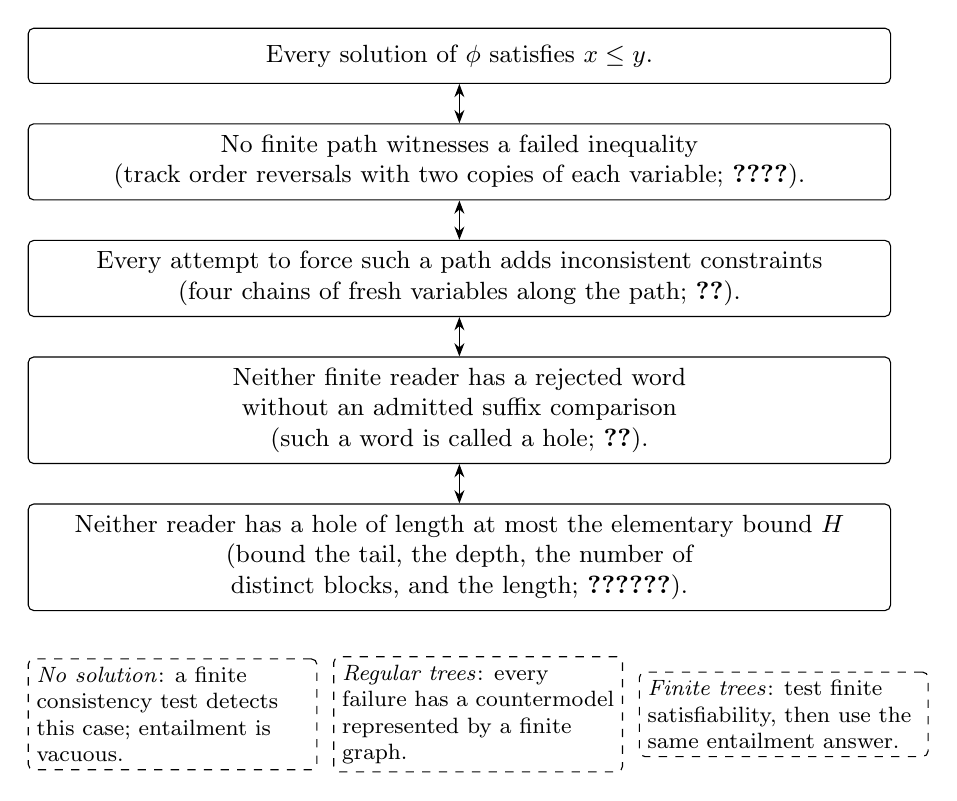
\begin{tikzpicture}[
    node distance=5mm,
    >=Stealth,
    redbox/.style={draw, rounded corners=2pt, align=center, text width=0.88\linewidth,
                 inner sep=4pt, minimum height=7mm, font=\small},
    domainbox/.style={draw, dashed, rounded corners=2pt, align=flush left,
                 text width=0.285\linewidth, inner sep=3pt,
                 font=\footnotesize}]
  \node[redbox] (ent) {Every solution of $\phi$ satisfies \mbox{$x\le y$}.};
  \node[redbox, below=of ent] (unsafe)
    {No finite path witnesses a failed inequality\\
     (track order reversals with two copies of each variable; \cref{sec:unsafe,sec:signed}).};
  \node[redbox, below=of unsafe] (spine)
    {Every attempt to force such a path adds inconsistent constraints\\
     (four chains of fresh variables along the path; \cref{thm:four-spine}).};
  \node[redbox, below=of spine] (hole)
    {Neither finite reader has a rejected word without an admitted suffix comparison\\
     (such a word is called a hole; \cref{thm:holes}).};
  \node[redbox, below=of hole] (short)
    {Neither reader has a hole of length at most the elementary bound $H$\\
     (bound the tail, the depth, the number of distinct blocks, and the length; \cref{sec:tail,sec:depth,sec:search}).};
  \draw[<->] (ent) -- (unsafe);
  \draw[<->] (unsafe) -- (spine);
  \draw[<->] (spine) -- (hole);
  \draw[<->] (hole) -- (short);
  \node[domainbox, below=6mm of short.south west, anchor=north west] (unsat)
    {\emph{No solution}: a finite consistency test detects this case;
     entailment is vacuous.};
  \node[domainbox, right=2mm of unsat] (reg)
    {\emph{Regular trees}: every failure has a countermodel represented by a finite graph.};
  \node[domainbox, right=2mm of reg] (fin)
    {\emph{Finite trees}: test finite satisfiability, then use the same entailment answer.};
\end{tikzpicture}
\caption{The reduction for a satisfiable system $\phi$. Each double arrow is
an equivalence. The dashed boxes explain the satisfiability test and the
transfers to regular and finite trees.}
\Description{Five boxes link entailment to the absence of a finite counterexample path,
the inconsistency of constraints forcing that path, the absence of reader holes,
and a bounded search. Three dashed boxes cover unsatisfiable systems and the
two restricted tree domains.}
\label{fig:overview}
\end{figure}

\paragraph{Why Entailment Is Hard and What Makes It Decidable}
A failed tree inequality can be witnessed by a finite path, written as a
word over argument positions. After variance is accounted for, a word $w$
is \emph{left unsafe} if, in some solution, $x$ has a top leaf on a prefix
of $w$ but $y$ has none, and \emph{right unsafe} if $y$ has a bottom leaf on
a prefix of $w$ but $x$ has none. Entailment fails exactly when some word
is left or right unsafe.

Suffix comparisons arise when constraints connect subtrees at different
cuts of this path. In the covariant case, let $s<e$ be cuts of $w$, and
suppose that some input variable lies above the subtree of $x$ at cut $e$
and below the subtree of $y$ at cut $s$. Every top leaf of $x$ on $w$ then
lies at or beyond cut $e$, so the subtree of $x$ at cut $e$ has a top leaf
on a prefix of the remaining suffix $w[e:]$. The variable passes such a
leaf up to the subtree of $y$ at cut $s$, again on a prefix of $w[e:]$. If
$w[e:]$ is a prefix of $w[s:]$, this leaf of $y$ lies on $w$, so $w$ is not
left unsafe after all. A pair of cuts $s<e$ with $w[e:]$ a prefix of
$w[s:]$ is a \emph{comparison} of $w$; equivalently, $w[s:]$ has period
$e-s$. Under variance, comparing a subtree of $x$ with a subtree of its own
signed copy gives an analogous obstruction.

For example, take a binary covariant constructor, the single literal
$f(y,x)\le y$, and the query $x\le y$. In every solution $y\ne\Bot$, and
whenever $y$ is a constructor, it lies below its own $0$-child and $x$ lies
below its $1$-child. Hence, if $y$ has a bottom leaf on a word $w$, then
$w=0^i1z$, the nodes of $y$ along $0^i$ are constructors, and the subtree
of $y$ at cut $i+1$ lies above $x$. This is the order dual of the situation
above, with cuts $0<i+1$ and $x$ itself as the connecting variable: the
bottom leaf of $y$ lies in that subtree on a prefix of $z$, and it forces a
bottom leaf of $x$ on a prefix of $z$. If $(0,i+1)$ is a comparison, that is, if
$z$ is a prefix of $w$, then $x$ also has a bottom leaf on $w$, and $w$ is
not right unsafe. Conversely, a word $0^i1z$ for which $(0,i+1)$ is not a
comparison is right unsafe (\cref{sec:general-holes}). The right-unsafe
words must therefore avoid a periodic comparison between their suffixes,
and they do not form a regular set: those in $0^*10^*$ are exactly the
words $0^i10^j$ with $j>i$.

A finite \emph{reader} records the constraints along a word. It
\emph{rejects} a word when none of the tests at single cuts rules the word
out, so rejection marks a candidate counterexample word. A comparison is
\emph{admitted} when its two reader states certify an obstruction of the
kind just described. A \emph{hole} is a rejected word with no admitted
comparison. For a satisfiable system, the holes of two such readers are
exactly the left-unsafe and the right-unsafe words. Ordinary loop deletion
can preserve the final reader state while creating a new admitted
comparison (\cref{ex:loop-deletion}). Preserving the run is therefore
insufficient.

Readers constructed from subtype constraints satisfy a
\emph{rejected-path property}: the rejected cuts of a word form an
interval, and every admitted comparison ends no later than the first
rejected cut. The reason is semantic. In the left label reader, at a rejected
cut, no variable that the constraints place above the subtree of $x$ is
bounded above by a constructor. From the next cut on, the constraints
therefore bound the subtree of $x$ by no variable at all, whereas every
admission needs such a bound at its later cut (\cref{sec:interface}). The
right label reader is dual. \Cref{tab:reader-hypotheses} records which bounds
need this property.

\paragraph{From Constraints to a Finite Search}
To handle variance, normalization exchanges $\Bot$ and $\Top$ at paths
of odd polarity, that is, paths with an odd number of contravariant edges.
Positive and negative copies of each variable then give a covariant
system; the solutions that matter assign dual trees to the two copies. We
obtain such a solution by selecting labels on a constructor shape common to both
copies. Four chains of fresh constraints along the candidate word, called
\emph{spines}, impose the two unsafety conditions and their signed
counterparts. Classifying the inconsistencies of this extension gives the
reader. For $k$ input variables, a state stores two sets of the $2k$ signed
variables and one bit recording an earlier obstruction, so there are
$N=2\cdot4^{2k}=2^{4k+1}$ states.

The finite search uses three bounds.
\begin{enumerate}[leftmargin=*]
\item \emph{Tail} (\cref{sec:tail}). If a reader with the rejected-path
  property has a hole, then it has one whose \emph{rejected tail}, the part
  after the first rejected cut, has length linear in $N$. If a cycle of
  rejected states allows a second letter, repeating the cycle and then
  taking the other letter breaks every relevant period; otherwise
  continuation within rejected states is forced, and a long periodic tail
  can be truncated.
\item \emph{Depth} (\cref{sec:depth}). For every reader, a suffix
  comparison of a rejected word that joins equal states has gap at most
  that word's rejected-tail length. Cutting a word at the occurrences of
  its last letter, and repeating this on the resulting word of blocks,
  gives a hierarchy of block decompositions. The gap bound limits its
  depth, quadratically in $N$ when the tail is linear in $N$.
\item \emph{Length} (\cref{sec:search}). For every reader, a hole of
  bounded depth can be shortened. Merging interchangeable letters bounds
  the number of distinct blocks at each positive level, and the blocks of
  a level are then shortened simultaneously. Finite summaries preserve
  transitions, admissions, and block equalities.
\end{enumerate}
Together, the three bounds give a hole whose length is triply exponential
in $k$ whenever some hole exists. For arbitrary readers, the remaining
question is whether a computable rejected-tail bound exists
(\cref{sec:general-holes}).

\paragraph{Contributions and Scope}
\begin{itemize}[leftmargin=*]
\item A decision procedure for one constructor of any finite arity and
  variance over arbitrary, regular, and finite trees (\cref{thm:main}).
\item A reduction of non-entailment to holes of finite readers
  (\cref{sec:variance,sec:spines,sec:holes}). Closure-based satisfiability
  characterizations are classical
  \citep{KozenPalsbergSchwartzbach94,PalsbergOKeefe95,PalsbergWandOKeefe97}.
  The new semantic ingredients are a least constructor shape common to the
  two signed copies of each variable, the selection of labels on that shape
  to handle variance, and the four-spine analysis that defines the reader.
\item Alphabet-generic bounds on tails, depth, and length
  (\cref{sec:tail,sec:depth,sec:search}); the latter two apply to every
  reader. For readers with the rejected-path property, they bound the
  length of a shortest hole doubly exponentially in a polynomial of $N$,
  hence triply exponentially in $k$ for the label readers
  (\cref{thm:hole-decision}).
\item Countermodel transfers (\cref{sec:decision,app:domains}), including
  coincidence of finite and arbitrary-tree entailment whenever a finite
  solution exists. That solution excludes cycles in the base constraints;
  the spines preserve this exclusion and permit a finite countermodel.
\item Complexity bounds in each domain (\cref{sec:complexity}). A search
  that stores one level of the block hierarchy at a time places entailment in
  2-EXPSPACE and 3-EXPTIME (\cref{thm:complexity}); constructors of arity at
  most one admit stronger bounds (\cref{app:small-arity}). For a covariant
  constructor of every fixed arity
  $n\ge2$, entailment is PSPACE-hard (\cref{thm:cx-hard}), which for $n=2$
  reproves the non-structural hardness theorems of \citet{HengleinRehof98},
  and shortest holes can have length $2^{\Omega(k)}$ (\cref{prop:cx-length}).
\item An end-to-end Lean~4 mechanization, for flat constraints, of the three
  procedures and their correctness, and of the combinatorial content of the
  complexity bounds: the summary search with its configuration bound, the
  one-letter bound, the hardness reduction, and the exponentially long holes
  (\cref{sec:mechanization,app:lean}).
\item A counterexample to Proposition~16 of \citet{NiehrenPriesnitz03}
  (\cref{app:np03}); \cref{sec:errata} explains which published proofs
  depend on that proposition.
\end{itemize}
The proof does not use the cap-automaton construction or its
back-translation from \citet{NiehrenPriesnitz03}. An earlier version of this
work proved the binary covariant case through a mechanized form of the
forward cap-automaton characterization; \cref{sec:experience} describes that
proof and explains why we replaced it.

\paragraph{How to Read This Paper}
\Cref{sec:background} fixes the semantics and the input language.
\Cref{sec:variance,sec:spines,sec:holes} turn subtype constraints into a
word problem. They build on one another and end with the label readers and
their rejected-path property. \Cref{sec:tail,sec:depth,sec:search} solve
that word problem; their principal results are the tail, depth, and
bounded-length theorems (\cref{thm:brt,thm:depth,thm:search}). From the
earlier sections they use only the definitions of comparisons, readers, and
holes and the rejected-path property, all in \cref{sec:holes}, so a reader
interested mainly in the word combinatorics can start there.
\Cref{sec:decision} assembles the decision procedures and the domain
transfers. \Cref{sec:complexity} replaces the explicit enumeration of words
by a search over summaries; it uses the lettered monitors and summaries of
\cref{sec:search}, the reader construction of \cref{sec:holes}, and the
statements of \cref{sec:decision}. \Cref{sec:mechanization} describes the
Lean artifact, \cref{sec:related} discusses related work,
\cref{sec:experience} compares the present proof with the earlier binary
proof, and \cref{sec:future} discusses open problems. The appendices supply
the spine proofs, the preservation arguments for cores and compression, the
domain transfers, the resource accounting and lower-bound details for the
complexity results, and the correspondence with the Lean development; they
end with a navigation table of proof distinctions and the counterexample to
NP03's Proposition~16.

\section{Background}
\label{sec:background}

\subsection{Words and Trees}\label{sec:words}
Fix an arity $n\in\mathbb N$, the child alphabet $\Dir=\{0,\ldots,n-1\}$,
and a variance map
$c:\Dir\to\{0,1\}$. Here $0$ means covariant and $1$ contravariant.
The signature contains exactly $\Bot$, $\Top$, and one constructor $f$ of arity $n$.
A \emph{cut} of a word $w$ of length $m$ is an integer $0\le j\le m$;
cut $j$ separates its first $j$ letters from the remaining suffix.
Write $w[i]$ for its letter at position $i$, with indices starting at $0$
and $0\le i<m$. Words are finite; $\eps$ is the empty word, concatenation is juxtaposition,
$u\pre w$ means that $u$ is a prefix of $w$, and $w[:j]$, $w[j:h]$, $w[j:]$
are its prefix, factor, and suffix at the indicated cuts. For example, over
$\{0,1\}$, $010[:2]=01$ and $010[1:]=10$. A positive integer $\varpi$ is a
\emph{period} of $w$ when $w[i]=w[i-\varpi]$ for $\varpi\le i<|w|$.
For a set $L$ of words, $\pr(L)$ is the set of prefixes of its members, and
$\pr(v)$ abbreviates $\pr(\{v\})$. For a nonempty root word $\rho$,
$\pr(\rho^*)$ thus consists of the prefixes of its finite powers; these are
exactly the finite prefixes of $\rho^\omega$.

\begin{lemma}[Periodic prefixes]\label{lem:periodic}
For $\rho\ne\eps$, $u\in\pr(\rho^*)$ iff $u\pre\rho^\omega$ iff $u\pre\rho u$.
\end{lemma}
\begin{proof}
The first equivalence follows by choosing a sufficiently long power. If
$u\pre\rho^\omega$, then both $u$ and $\rho u$ prefix the same infinite word.
Conversely, $u\pre\rho u$ either gives $u\pre\rho$, or lets us cancel an
initial $\rho$ and repeat on a shorter word.
\end{proof}

The \emph{polarity} of a path counts contravariant positions modulo two:
\begin{equation}\label{eq:g1}
 p(w)=\bigoplus_{j<|w|}c(w[j]),\qquad p(\eps)=0,\qquad p(uv)=p(u)\oplus p(v).
\end{equation}
Occurrences are counted with multiplicity: if $c(0)=1$ and $c(1)=0$, then
$p(0)=1$, $p(00)=0$, and $p(010)=0$.

A \emph{tree} is a partial labeling $t:\Dir^*\rightharpoonup\{\Bot,f,\Top\}$,
with a defined root and prefix-closed domain, such that
\begin{equation}\label{eq:g2}
 wi\in\operatorname{dom}(t)\quad\Longleftrightarrow\quad t(w)=f
 \qquad(i\in\Dir).
\end{equation}
The \emph{extreme labels} are $\bot$ and $\top$. They label leaves;
an $f$-node has $n$ children, so $f()$ is also a leaf at arity zero.
Write $f(t_i)_{i\in\Dir}$ for a constructor tree. A subtree at $\eta$ has
labeling $w\mapsto t(\eta w)$, when $\eta$ belongs to the domain.
For example, the finite binary tree $f(\Bot,\Top)$ has domain
$\{\eps,0,1\}$. The full constructor tree $F=f(F,\ldots,F)$ is infinite
when $n>0$ and is $f()$ when $n=0$.

Let $\Trees$ contain all trees, $\Trees_{\mathrm{fin}}$ those with finite
domain, and $\Trees_{\mathrm{reg}}$ those with finitely many distinct rooted
subtrees. A tree is regular iff it is the unfolding of a finite labeled graph
with $n$ ordered outgoing edges at each constructor node; for the forward
direction, take the graph of its finitely many distinct subtrees. The tree $F$ has a one-state
graph. Every finite tree is regular, but $F$ shows that the converse fails
at positive arity. At arity zero, the only trees are $\Bot,f(),\Top$.

\subsection{Non-Structural Subtyping}
Order the labels by $\Bot<f<\Top$. Define
\begin{equation}\label{eq:g3}
 t\le_c u\quad\Longleftrightarrow\quad
 \forall w\in\operatorname{dom}(t)\cap\operatorname{dom}(u),\quad
 \begin{cases}t(w)\le u(w),&p(w)=0,\\u(w)\le t(w),&p(w)=1.\end{cases}
\end{equation}
For $c=0$, write $\le$ and call the order \emph{covariant}.
The order is non-structural because $\Bot\le_c t\le_c\Top$ holds even for
trees of different shapes. For binary products $c(0)=c(1)=0$; for arrows
$c(0)=1,c(1)=0$, and the usual rule is
$f(a_0,a_1)\le_c f(b_0,b_1)$ iff $b_0\le_c a_0$ and $a_1\le_c b_1$.
For instance, $f(\Top,\Bot)\le_c f(\Bot,\Top)$ for arrows.

For a relation $R$ on trees, define the textbook one-step rule
\begin{equation}\label{eq:g4}
\begin{split}
 \operatorname{Step}_c(R)(t,u)\quad\Longleftrightarrow\quad& t=\Bot\ \lor\ u=\Top\\
 &\lor\ \exists\vec a,\vec b\;[t=f(\vec a)\land u=f(\vec b)\land
 \forall i\;\begin{cases}R(a_i,b_i),&c(i)=0,\\R(b_i,a_i),&c(i)=1.\end{cases}]
\end{split}
\end{equation}
Then $\le_c=\nu R.\operatorname{Step}_c(R)$, the \emph{greatest fixed point}:
the largest relation preserved by this rule. To prove it, compare roots
in \eqref{eq:g3} and apply \eqref{eq:g1} to the children; this shows that
\eqref{eq:g3} is a fixed point. Conversely, if $R\subseteq\operatorname{Step}_c(R)$,
induction on a common path proves \eqref{eq:g3} for every pair in $R$.
A contravariant first letter exchanges the trees and toggles polarity; a
leaf case leaves only the root comparison. The greatest fixed point is
necessary: at positive arity $F\le_c F$, whereas the least fixed point
cannot justify this comparison by finitely many unfoldings. On finite
trees, the same rule is the usual inductive order. The relation is a partial
order, as also follows from normalization and the pointwise characterization
in \eqref{eq:g11}.

\subsection{Constraints, Solutions, and Entailment}
Let $V$ be a finite set of $k$ variables containing $x,y$. A \emph{flat constraint system} $\phi$ is a finite conjunction of literals
\begin{equation}\label{eq:g5}
 z\le f(a_i)_i,\qquad f(a_i)_i\le z,\qquad z=\Bot,\qquad z=\Top,
\end{equation}
where each $a_i$ is a variable. An assignment $\sigma:V\to\mathcal D$, for
$\mathcal D\in\{\Trees,\Trees_{\mathrm{reg}},\Trees_{\mathrm{fin}}\}$, is a
\emph{solution} if it satisfies all literals, interpreting inequalities by
$\le_c$. Write $\Sat_{\mathcal D,c}(\phi)$ for existence of a solution. Define
\begin{equation}\label{eq:g6}
 \phi\models_{\mathcal D,c}x\le y\quad\Longleftrightarrow\quad
 \forall\sigma:V\to\mathcal D,\quad\sigma\models_c\phi\Longrightarrow
 \sigma(x)\le_c\sigma(y).
\end{equation}
Omit $\mathcal D$ for arbitrary trees, and use $\mathrm{reg}$ and $\mathrm{fin}$
for the other domains; omit $c$ as well in the covariant case.
Satisfiability asks for one solution; entailment asks
about every solution. A \emph{countermodel} is a solution that violates
the query. An unsatisfiable system entails every query.
For example, $x\le f(a_i)_i$ and $f(a_i)_i\le y$ entail $x\le y$.
With distinct variables they do not entail $y\le x$: set $x=\Bot,y=\Top$.
For a binary covariant constructor, $f(x,x)\le x\le f(x,x)$ has a regular
infinite solution but no finite solution.
The query $x\le y$ is a variable inequality. It is accepted directly and is
not a literal of \eqref{eq:g5}; general systems and queries reduce to this
form as follows.

\begin{proposition}[Flattening]\label{prop:flattening}
At positive arity, any finite system of inequalities between finite type
expressions, with a type-expression query, reduces to the flat syntax
\eqref{eq:g5} and a variable query. Solutions correspond under projection
in each of the three tree domains. At arity zero, such entailments are
decidable by enumerating assignments in $\{\bot,f(),\top\}$.
\end{proposition}
\begin{proof}
Give each nonvariable subexpression a fresh name. For a constructor
subexpression, impose both flat bounds between its name and the constructor
applied to the names of its children; for a constant, impose its constant
literal. Antisymmetry forces each name to denote its subexpression.
Replace each original inequality, and the query, by the variable inequality
between the names of its two sides. The query is now a variable query.

A variable inequality $u\le v$ in the system is not a literal of
\eqref{eq:g5}, but at positive arity it can be expressed with fresh
auxiliaries. Choose a child $i$, put $u,v$ in the $i$th coordinates of
vectors $\vec a,\vec b$ (exchanged if $c(i)=1$), use a common filler
variable in the other coordinates, and add the two literals
$f(\vec a)\le z\le f(\vec b)$ with a fresh \emph{sandwich variable} $z$.
A solution extends by evaluating subexpressions and taking $z$ to be
$f(\vec a)$. Conversely, the two literals give $f(\vec a)\le_c f(\vec b)$,
and decomposing it at child $i$ gives $u\le_c v$.
These extensions use only constants and finitely many constructor
applications, which preserve finite and regular trees. At arity zero, all
expressions evaluate in the displayed three-element chain, and the sandwich
encoding is unavailable.\footnote{Every flat literal
then concerns one variable. Solution sets, even after existential projection,
are products of unary sets; the order on $\bot<f()<\top$ is not such a product.}
\end{proof}
This reduction explains the mathematical scope; the exported formal
procedures take the flat syntax directly (\cref{app:lean}).

\subsection{Normalization}\label{sec:normal}
Normalization moves all order reversals from the comparison rule into the
leaf labels: after it, every path is compared covariantly.
Define \emph{tree duality} $\mathfrak d(t)$ by exchanging $\bot$ and
$\top$ and leaving every $f$-label unchanged, including the nullary
constructor $f()$. For $q\in\{0,1\}$, define $H_qt$ on the same domain as
$t$, exchanging $\bot$ and $\top$ in its label at $w$ precisely when
$q\oplus p(w)=1$. The following lemma shows that $H_0$ turns $\le_c$ into
the covariant order.

\begin{lemma}[Normalization]\label{lem:normalization}
\begin{equation}\label{eq:g9}
H_q f(t_i)_i=f(H_{q\oplus c(i)}t_i)_i,\qquad
 H_1=\mathfrak d H_0,\qquad H_0H_0=\mathrm{id},
\end{equation}

\begin{equation}\label{eq:g10}
t\le_c u\quad\Longleftrightarrow\quad H_0t\le H_0u.
\end{equation}

\end{lemma}
\begin{proof} Exchanging the extreme labels preserves \eqref{eq:g2}. At a child path $iw$, \eqref{eq:g1} gives
the sign in \eqref{eq:g9}; flipping twice proves the involution identities.
At every common path, exchanging the extreme labels reverses their order. Thus the comparison in
\eqref{eq:g3} is exactly the covariant comparison after applying $H_0$, proving \eqref{eq:g10}.
In particular, $H_0$ is an order isomorphism to the covariant tree order.
Both $H_q$ and $\mathfrak d$ preserve finite domains. They preserve regularity:
in a finite graph, attach one polarity bit to each node and update it on an
edge labeled $i$ by xor with $c(i)$. \end{proof}

\subsection{Unsafe Words and Sides}\label{sec:unsafe}
For a covariant tree $t$, define its \emph{constant leaf extension}
$\widehat t:\Dir^*\to\{\bot,f,\top\}$ by following a word until its
end or the first leaf, and then retaining that leaf's label. Thus
$\widehat t(w)=\top$ exactly when some prefix of $w$ is a $\top$-leaf
of $t$; the analogous assertion holds for $\bot$.

\begin{lemma}[Leaf-extension characterization]\label{lem:leaf-extension}
The covariant order has the characterization

\begin{equation}\label{eq:g11}
t\le u\quad\Longleftrightarrow\quad
 \forall w\quad\widehat t(w)\le\widehat u(w).
\end{equation}

\end{lemma}
\begin{proof} The reverse implication follows by considering common domain
paths. For the forward implication, follow both trees along $w$. Until a
leaf is reached, labels compare by hypothesis. If the left tree stops at
$\bot$, or the right at $\top$, the extended comparison holds forever.
If the left stops at $\top$, the right must also be $\top$ at that common
node; if the right stops at $\bot$, the left must also be $\bot$.
Otherwise, both reach the end and the original comparison applies. \end{proof}

For a tree $t$ ordered by $\le_c$, put

\begin{equation}\label{eq:g12}
\operatorname{Pref}_c^+(t,w):\Longleftrightarrow\widehat{H_0t}(w)=\top,
 \qquad
 \operatorname{Pref}_c^-(t,w):\Longleftrightarrow\widehat{H_0t}(w)=\bot.
\end{equation}

We say that $t$ has a \emph{top prefix} along $w$ if
$\operatorname{Pref}_c^+(t,w)$, and a \emph{bottom prefix} along $w$ if
$\operatorname{Pref}_c^-(t,w)$.
Thus a top prefix is an actual top leaf at an even-polarity prefix of $w$,
or an actual bottom leaf at an odd-polarity prefix. Its polarity is measured
at that prefix, not at a later point past the leaf.
A word $w$ is \emph{left unsafe} for an assignment $\sigma$ if
$\operatorname{Pref}_c^+(\sigma x,w)$ and not $\operatorname{Pref}_c^+(\sigma y,w)$, and
\emph{right unsafe} for $\sigma$ if
$\operatorname{Pref}_c^-(\sigma y,w)$ and not $\operatorname{Pref}_c^-(\sigma x,w)$.
It is left (right) unsafe for $(\phi,x,y)$ if it is left (right) unsafe for
some solution of $\phi$.

By \eqref{eq:g10}--\eqref{eq:g11},

\begin{equation}\label{eq:g13}
\phi\not\models_c x\le y
 \quad\Longleftrightarrow\quad
 \text{some word is left unsafe or right unsafe}.
\end{equation}

Indeed, the only failures of order in the three-element label chain are a
left top against a non-top, or a right bottom against a non-bottom. The same
argument shows, for each assignment $\sigma$, that
$\sigma(x)\not\le_c\sigma(y)$ iff some word is left or right unsafe for
$\sigma$.


\begin{example}[Running arrow system]\label{ex:running-arrow}
Take $c=(1,0)$, variables $x,y,a,b$, and the three flat literals
\[
 \phi=\{x\le f(a,b),\ f(a,b)\le x,\ y\le f(a,b)\}.
\]
The first two force $x=f(a,b)$, so every solution has $y\le_c x$.
The converse query fails: the finite assignment
\[
 \sigma(a)=\Bot,\quad \sigma(b)=\Top,\qquad
 \sigma(x)=f(\Bot,\Top),\quad \sigma(y)=f(\Top,\Bot)
\]
solves $\phi$, but $\sigma(x)\not\le_c\sigma(y)$.
As \cref{fig:arrow-witness} shows, normalization gives
$H_0\sigma(x)=f(\Top,\Top)$ and $H_0\sigma(y)=f(\Bot,\Bot)$.
Thus $w=0$ witnesses both sides of unsafety: $x$ has a top prefix and
$y$ does not, while $y$ has a bottom prefix and $x$ does not.
The same assignment witnesses both sides for $00$: the leaves are reached
at $0$, whose polarity is $1$, even though $p(00)=0$.
We reuse this system with the failing query $x\le y$ below.
\end{example}

\begin{figure}[t]
\centering
\begin{tikzpicture}[x=10mm,y=8mm,>=Stealth,
    every node/.style={font=\small,inner sep=2pt}]
  \node (x) at (0,0) {$f$};
  \node (x0) at (-1,-1.2) {$\Bot$};
  \node (x1) at (1,-1.2) {$\Top$};
  \node[above=2mm of x] {$\sigma(x)$};
  \draw (x) -- node[left,font=\scriptsize] {$0\;(-)$} (x0);
  \draw (x) -- node[right,font=\scriptsize] {$1\;(+)$} (x1);
  \node at (2.6,-0.5) {$\not\le_c$};
  \node (y) at (5.2,0) {$f$};
  \node (y0) at (4.2,-1.2) {$\Top$};
  \node (y1) at (6.2,-1.2) {$\Bot$};
  \node[above=2mm of y] {$\sigma(y)$};
  \draw (y) -- node[left,font=\scriptsize] {$0\;(-)$} (y0);
  \draw (y) -- node[right,font=\scriptsize] {$1\;(+)$} (y1);
  \draw[->] (0,-1.8) -- (0,-2.5) node[midway,right] {$H_0$};
  \draw[->] (5.2,-1.8) -- (5.2,-2.5) node[midway,right] {$H_0$};
  \node at (0,-2.9) {$f(\Top,\Top)$};
  \node at (2.6,-2.9) {$\not\le$};
  \node at (5.2,-2.9) {$f(\Bot,\Bot)$};
\end{tikzpicture}
\caption{The countermodel of \cref{ex:running-arrow}. The argument edge $0$ (the arrow's domain)
reverses the order: $x\le_c y$ would require $\Top\le_c\Bot$ there.
Normalization flips that edge's leaf labels, exposing the top-prefix and
bottom-prefix failures at the same word $0$.}
\Description{Two binary constructor trees. The x tree has bottom on child zero
and top on child one; the y tree has top on child zero and bottom on child one.
Child zero is contravariant and child one covariant. Arrows below show
normalization to two top leaves for x and two bottom leaves for y.}
\label{fig:arrow-witness}
\end{figure}


\FloatBarrier
\subsection{Notation at a Glance}\label{sec:notation}
The following table collects the main notation, including symbols
introduced later, grouped by the part of the paper that introduces them.
In particular, the three dual operations have different input and output
types.
\begingroup
\small
\begin{longtable}{@{}>{\raggedright\arraybackslash}p{.21\linewidth}>{\raggedright\arraybackslash}p{.28\linewidth}>{\raggedright\arraybackslash}p{.44\linewidth}@{}}
\toprule
Symbol & Type & Reading or effect\\
\midrule
\endfirsthead
\toprule
Symbol & Type & Reading or effect\\
\midrule
\endhead
\bottomrule
\endfoot
\multicolumn{3}{@{}l}{\emph{Semantics and constraints (\cref{sec:background,sec:variance,sec:spines})}}\\
$\Trees$, $\Trees_{\mathrm{reg}}$, $\Trees_{\mathrm{fin}}$ & sets of trees & Arbitrary, regular, and finite trees; $\mathcal D$ ranges over these domains.\\
$V$, $V^\pm$, $\sigma$ & variable sets; assignment & Original and signed variables; a tree for each variable.\\
$\phi$, $\psi$, $\chi$ & finite constraint systems & Original system, signed translation, and a generic covariant system.\\
$k$ & integer & Number of input variables (never a block count).\\
$\Dir$, $c$, $p$ & alphabet; $\Dir\to\{0,1\}$; $\Dir^*\to\{0,1\}$ & Child positions, their variances, and path polarity.\\
$w[i]$, $w[:j]$, $w[j:]$ & letter; word; word & Letter at position $i$; prefix and suffix at cut $j$.\\
$u\pre w$, $\pr(L)$ & relation on words; set of words & Prefix; all prefixes of words in $L$, with $\pr(v)=\pr(\{v\})$.\\
$\mathfrak d$ & $\Trees\to\Trees$ & Tree duality: exchange $\bot,\top$, retain $f$.\\
$H_q$ & trees under $\le_c$ $\to$ covariant trees & Normalize labels using $q\oplus p(w)$.\\
$\operatorname{Pref}^\pm_c(t,w)$ & truth value & Top ($+$) or bottom ($-$) prefix of $t$ along $w$.\\
$\flip$ & $V^\pm\to V^\pm$ & Variable flip: complement the sign.\\
$S$ & signed assignments $\to$ signed assignments & Assignment involution: $(S\sigma)(v)=\mathfrak d(\sigma(\flip v))$; fixed witnesses are $S$-fixed.\\
$\theta$; $X_\theta$, $Y_\theta$ & side; signed variables & Left or right side and its two query roots in $\psi$: $(x^+,y^+)$ on the left, $(y^-,x^-)$ on the right.\\
$D_\chi$ & relation on variables & Reflexive, transitive decomposition closure.\\
$\Up$, $\Lo$ & word $\times$ variable $\times$ variable $\to$ truth value & Supported upper and lower path bounds.\\
$\emb_b(\eta,t)$ & tree & Embed $t$ at path $\eta$, with off-path filler $b$.\\
$\ell_f,u_f,u_\bot$ & predicates on pairs of a variable and a path & Lower constructor, upper constructor, and upper bottom support.\\
$\Psi^4_w$; $P_j$, $Q_j$, $Y_j$, $W_j$ & system; signed variables & Four-spine extension along $w$ and its spine variables at cut $j$.\\
$U_j,L_j$; $U^R_j,L^Z_j$ & sets of signed variables & Variables reached by upper and lower path bounds at cut $j$, from $x^+$ and $y^+$, or from the spine roots $R_0$ and $Z_0$.\\
\midrule
\multicolumn{3}{@{}l}{\emph{Readers and holes (\cref{sec:holes,sec:tail,sec:depth,sec:decision})}}\\
$(\mathcal M,\Adm,\Rej)$, $N$ & reader; integer & Deterministic automaton with admission relation and rejected states; its number of states.\\
$\mathcal M_\theta$, $\Adm_\theta$, $\Rej_\theta$ & reader & Left or right label reader: the label reader of \cref{sec:label-reader} on side $\theta$.\\
$E_i$, $G_i$ & maps on sets of signed variables & One-letter updates of the upper and lower sets.\\
$(s,e)$ & pair of cuts & Comparison when $s<e$ and $w[e:]\pre w[s:]$.\\
$q_j$, $\Rej$, $\Adm$ & state; set of states; relation on states & Reader run, rejection, and admission.\\
$J(w)$, $r(w)$ & integers & First rejected cut and rejected-tail length $|w|-J(w)$.\\
hole; fixed witness & word; assignment & Rejected word without admitted comparison, for a satisfiable system an unsafe word; $S$-fixed solution showing unsafety along a word. \emph{Witness} always means the latter.\\
$B$, $d$, $H$ & integers & Tail bound $4N-2$, depth bound $2N(B+1)-1$, and length bound $\holeBound(N,d)$ (\cref{thm:hole-decision}).\\
\midrule
\multicolumn{3}{@{}l}{\emph{Hierarchies and compression (\cref{sec:depth,sec:search,sec:complexity})}}\\
$u_j$, $\ell_j$, $\Cores_j$, $\Supp_j$ & word; letter; set of cuts; set of states & Hierarchy level, marker, ordinary cores, and their reader states (state support).\\
$\mathcal M_j$, $\triangleright$, $\star$ & lettered monitor; label; state & Derived monitor, start label, and new derivative start state.\\
$\Tfin$, $\Lambda$, $\Lfin$ & predicate; two relations on labels & Final target, nonterminal admission, and terminal admission.\\
$\mathcal A_i$, $g_i$ & set of letters; integer & Level-$i$ dictionary (letters of $u_i$) and its size.\\
$\Pi_i$, $Z_i$ & set of letters; set of states & Protected letters and monitor states in use at level $i$.\\
$\mathcal E_j$ & set of letters & Letter support kept at level $j$ during shortening.\\
$\Delta$ & integer & Depth of the hole being shortened in \cref{sec:search}.\\
$\TyBound(N,d)$, $\AlBound(N,d)$, $\DictBound(N,d)$ & integers & Number of exchange types, allowance, and dictionary bound \eqref{eq:dictionary-constants}.\\
$h$, $\mathit{col}(N,h)$ & integers & Number of blocks (tracks) shortened together; column count of their summaries \eqref{eq:col}.\\
$\holeBound(N,d)$ & integer & Length bound for holes of depth at most $d$ \eqref{eq:holebound}.\\
dictionary-normal & property of holes & Normal form of \cref{lem:dictionary-normal-form}; unrelated to the normalization $H_q$.\\
\midrule
\multicolumn{3}{@{}l}{\emph{Complexity (\cref{sec:complexity})}}\\
$\insize{\phi}$ & integer & Size of the explicit input.\\
cycle clash & property of a system & $\Lo(\eta,a,a)$, $D_\chi(a,b)$ and $\Up(\eta,b,b)$ for a nonempty $\eta$; excludes finite solutions (\cref{sec:decision}).\\
$\mathcal W$, $\Gamma_{\mathcal W}$, $\Theta$ & lettered monitor; alphabet; summary & Current monitor of the summary search, its abstract letters $1,\ldots,h$, and a column summary determining the next monitor.\\
$\mathbb T$ & alphabet & Counter tokens $\{0,1,\#,\$\}$ of the long-hole construction.\\
$T_P$, $T_P^m$ & trees & Top-free tree with constructor positions $P$, and its truncation at depth $m$ with $\Top$ at the cut.\\
$\Phi^{(n)}(\mathcal A)$, $\mathcal A^\circ$ & system; automaton & Rejection system of an all-final automaton $\mathcal A$; all-final code of an automaton (hardness).\\
token encoding; $e$ & maps into $\{0,1\}^*$ & Binary encoding of counter tokens (long holes); letter doubling $a\mapsto0a$ (hardness).\\
\end{longtable}
\endgroup

\section{Signed Constraints and Fixed Witnesses}
\label{sec:variance}

We remove variance by giving each variable two signed copies. The copies
must denote dual trees; the assignment involution expresses this condition.
We then express each side of a failed query by a \emph{fixed witness}: a
solution of the signed system that is fixed by the assignment involution and
exhibits the failure along a given word. The four-spine construction of
\cref{sec:spines} will enforce such witnesses.

\subsection{The Signed System}\label{sec:signed}
Write $V^{\pm}=V\times\{0,1\}$, $v^+=v^0$, $v^-=v^1$, and define the
\emph{variable flip} $\flip(v^q)=v^{1-q}$. Translate $\phi$ to a covariant constraint system
$\psi=\phi^{\pm}$ as follows:

\begin{center}
\begin{tabular}{@{}lll@{}}
\toprule
Original literal & \multicolumn{2}{c}{Signed literals}\\
\midrule
$z\le f(a_i)_i$ & $z^+\le f(a_i^{c(i)})_i$ & $f(a_i^{1\oplus c(i)})_i\le z^-$\\
$f(a_i)_i\le z$ & $f(a_i^{c(i)})_i\le z^+$ & $z^-\le f(a_i^{1\oplus c(i)})_i$\\
$z=\bot$ & $z^+=\bot$ & $z^-=\top$\\
$z=\top$ & $z^+=\top$ & $z^-=\bot$\\
\bottomrule
\end{tabular}
\end{center}

\begin{lemma}[Signed correspondence]\label{lem:signed}
For an assignment $\sigma$ on signed variables define
$(S\sigma)(v)=\mathfrak d(\sigma(\flip v))$. The map $S$, called the
\emph{assignment involution}, is an involution and preserves solutions of $\psi$.
Moreover,

\begin{equation}\label{eq:g14}
\sigma\longmapsto \sigma^{\pm},\qquad \sigma^{\pm}(v^q)=H_q(\sigma v)
\end{equation}

is a bijection between solutions of $\phi$ and $S$-fixed solutions of
$\psi$.
\end{lemma}

\begin{proof} Tree duality $\mathfrak d$ reverses inequalities and commutes with
$f$. Applying it and $\flip$ exchanges the two literals in each row of
the table. This proves preservation by $S$; applying both involutions twice gives
$S^2=\mathrm{id}$. By \eqref{eq:g9}--\eqref{eq:g10},
\eqref{eq:g14} satisfies each translated pair and is fixed by $S$. Conversely, for
an $S$-fixed solution define $\sigma_0(v)=H_0(\sigma(v^+))$. The fixed-point
identity gives $\sigma(v^-)=\mathfrak d(\sigma(v^+))$, so \eqref{eq:g9} reconstructs \eqref{eq:g14}. Applying \eqref{eq:g10}
to the positive literal of each pair proves $\sigma_0\models_c\phi$.
The reconstruction also proves both inverse identities. \end{proof}


\subsection{Fixed Witnesses}\label{sec:fixed-witness}
Write $\theta\in\{\mathsf l,\mathsf r\}$ for the left and right sides;
$\mathsf l$-unsafe means left unsafe, and similarly on the right. Both sides
read the same signed system $\psi$, from different query roots:
\[
 (X_{\mathsf l},Y_{\mathsf l})=(x^+,y^+),\qquad
 (X_{\mathsf r},Y_{\mathsf r})=(y^-,x^-).
\]
The right side exchanges the roots and uses their negative copies, because
the two copies of a variable denote dual trees: a bottom prefix of $y$ is a
top prefix of $y^-$.

We call a covariant solution $\sigma\models\psi$ a \emph{fixed
witness} for $w$ on side $\theta$ if $S\sigma=\sigma$ and
\begin{equation}\label{eq:fixed-witness}
 \widehat{\sigma(X_\theta)}(w)=\top,\qquad
 \widehat{\sigma(Y_\theta)}(w)\ne\top.
\end{equation}
Here \emph{fixed} means fixed by the assignment involution $S$, not that
the word $w$ is held fixed.

\begin{lemma}[Fixed-witness criterion]\label{lem:fixed-witness}
For either side $\theta$, a word $w$ is $\theta$-unsafe iff it has a fixed
witness on side $\theta$.
\end{lemma}
\begin{proof}
By \cref{lem:signed}, the $S$-fixed solutions of $\psi$ are exactly the
assignments $\sigma_0^{\pm}$ for solutions $\sigma_0$ of $\phi$, with
$\sigma_0^{\pm}(v^+)=H_0(\sigma_0v)$ and, by \eqref{eq:g9},
$\sigma_0^{\pm}(v^-)=H_1(\sigma_0v)=\mathfrak d(H_0(\sigma_0v))$. For the left
side, \eqref{eq:fixed-witness} for $\sigma_0^{\pm}$ therefore says that
$\sigma_0(x)$ has a top prefix along $w$ and $\sigma_0(y)$ has none, which is
the definition of a left-unsafe word for $\sigma_0$. For the right side, tree
duality exchanges the labels $\bot$ and $\top$ at every node, so
$\widehat{\mathfrak d(t)}(w)=\top$ iff $\widehat t(w)=\bot$. Hence
\eqref{eq:fixed-witness} at the roots $y^-$ and $x^-$ says that $\sigma_0(y)$
has a bottom prefix along $w$ and $\sigma_0(x)$ has none, which is the
definition of a right-unsafe word for $\sigma_0$. Both equivalences include
paths that terminate before the end of $w$.
\end{proof}

\begin{example}[The signed running witness]\label{ex:running-signed}
For \cref{ex:running-arrow}, the six signed literals can be grouped as
\[
 \begin{gathered}
 x^+\le f(a^-,b^+),\qquad f(a^-,b^+)\le x^+,
 \qquad y^+\le f(a^-,b^+),\\
 f(a^+,b^-)\le x^-,\qquad x^-\le f(a^+,b^-),
 \qquad f(a^+,b^-)\le y^-.
 \end{gathered}
\]
The contravariant child uses the opposite sign; passing to the negative
root also reverses the inequality. The assignment of
\cref{ex:running-arrow} translates to
\[
\begin{array}{c|cccc}
 v&x&y&a&b\\\hline
 \sigma^{\pm}(v^+)&f(\Top,\Top)&f(\Bot,\Bot)&\Bot&\Top\\
 \sigma^{\pm}(v^-)&f(\Bot,\Bot)&f(\Top,\Top)&\Top&\Bot
\end{array}
\]
and each column consists of dual trees, so $S\sigma^{\pm}=\sigma^{\pm}$.
At $w=0$, the labels at $x^+$ and $y^+$ are $\Top$ and $\Bot$, giving the
left fixed witness. The labels at $y^-$ and $x^-$ are also $\Top$ and
$\Bot$, so the same assignment is the right fixed witness for this word.
\end{example}

A covariant solution need not itself be fixed. \Cref{sec:spines} constructs
a fixed solution from the least shape (\cref{sec:least}) of any consistent
system that is flip-closed and sign coherent (\cref{sec:closure}). Flip
closure means closure under reversing inequalities, flipping variables, and
exchanging constants. Sign coherence means that each constructor child has
the sign of its root, toggled by the variance of its position. Applying that
construction to an extension encoding \eqref{eq:fixed-witness} will preserve
the witness conditions as well as satisfaction.

\section{Closure and Spine Clashes}
\label{sec:spines}

This section turns unsafety of a fixed word $w$ into a syntactic test on
the constraints. By \cref{lem:fixed-witness}, $w$ is unsafe on a side
exactly when the signed system of that side has a solution that is fixed by
the assignment involution $S$ and satisfies two prefix conditions along $w$.
We encode these conditions, together with their sign duals, by an extension
$\Psi^4_w$ with four chains of fresh variables, the spines
(\cref{sec:spine}). Two facts are needed before the spines, and they fix
the order of this section. First, a covariant system is satisfiable exactly
when it has no label clash, a condition on its finite closure
(\cref{sec:closure,sec:least}). Second, a clash-free system that is
flip-closed and sign coherent has a solution fixed by $S$, obtained by
polarity selection on its least shape (\cref{sec:selector}). Together they
reduce unsafety of $w$ to the absence of a label clash in $\Psi^4_w$
(\cref{thm:four-spine}). We then express the closure of $\Psi^4_w$ through
the closure of the original system and two sets $U_j,L_j$ of old variables
at each cut (\cref{sec:bridge-formula}). Classifying the clashes in these
terms (\cref{sec:events}) yields tests at single cuts and tests on suffix
comparisons. \Cref{sec:holes} packages these tests as a finite reader with
the rejected-path property.

\subsection{Closure and Supported Path Bounds}\label{sec:closure}
For this subsection, let $\chi$ be any finite covariant constraint system over a
finite variable set $\Vars$. Its \emph{closure} $D_\chi$ is the least reflexive and
transitive relation satisfying, for every $i\in\Dir$,

\begin{equation}\label{eq:g21}
\frac{f(\vec a)\le u\in\chi\qquad D_\chi(u,v)\qquad
 v\le f(\vec b)\in\chi}{D_\chi(a_i,b_i)}.
\end{equation}

Repeatedly adding reflexive, transitive, and decomposition consequences
computes $D_\chi$: there are only $|\Vars|^2$ pairs. Induction on a derivation
proves soundness, $D_\chi(u,v)\Rightarrow \sigma(u)\le \sigma(v)$ for every solution.
For the decomposition step use the constructor case of \eqref{eq:g4}.

Define \emph{supported upper and lower path bounds} by

\begin{equation}\label{eq:g22}
\begin{aligned}
 \Up(\eps,u,v)&\iff D_\chi(u,v),\\
 \Up(i\eta,u,v)&\iff
 \exists z,\vec b\ [D_\chi(u,z)\land z\le f(\vec b)\in\chi
 \land\Up(\eta,b_i,v)],\\
 \Lo(\eps,u,v)&\iff D_\chi(u,v),\\
 \Lo(i\eta,u,v)&\iff
 \exists\vec a,z\ [f(\vec a)\le z\in\chi\land D_\chi(z,v)
 \land\Lo(\eta,u,a_i)].
 \end{aligned}
\end{equation}

In every solution, $\Up(\eta,u,v)$ says that the subtree of $u$ at
$\eta$, when present, is below $v$; $\Lo(\eta,u,v)$ says that $u$ is
below the subtree of $v$ there. The variable arguments follow the order of
the inequality: the path is on the first variable for $\Up$ and on the
last for $\Lo$.
To state soundness without assuming the path exists, let
$\emb_b(\eta,t)$ embed $t$ at $\eta$, putting the constant
tree $b$ in every off-path child. Then

\begin{lemma}[Path rules]\label{lem:path-rules}
In every solution of $\chi$,
\begin{equation}\label{eq:g23}
\begin{aligned}
 \Up(\eta,u,v)&\Longrightarrow
 \sigma(u)\le\emb_{\top}(\eta,\sigma(v)),\\
 \Lo(\eta,u,v)&\Longrightarrow
 \emb_{\bot}(\eta,\sigma(u))\le \sigma(v).
 \end{aligned}
\end{equation}

Composition and factorization, including empty factors, satisfy
\begin{equation}\label{eq:path-factors}
\begin{aligned}
\Up(\eta\tau,u,v)&\iff\exists a\;[\Up(\eta,u,a)\land\Up(\tau,a,v)],\\
\Lo(\eta\tau,u,v)&\iff\exists a\;[\Lo(\tau,u,a)\land\Lo(\eta,a,v)].
\end{aligned}
\end{equation}
At an empty factor the path judgment retains the closure relation
$D_\chi$, rather than requiring equality of its endpoints.
For later use, cancellation of a common path gives

\begin{equation}\label{eq:g24}
\begin{aligned}
 \Lo(\eta,a,z)\land
 \Up(\eta\tau,z,b)
 &\Longrightarrow\Up(\tau,a,b),\\
 \Lo(\eta\tau,a,z)\land
 \Up(\eta,z,b)
 &\Longrightarrow\Lo(\tau,a,b).
 \end{aligned}
\end{equation}

\end{lemma}
\begin{proof}
Induction on \eqref{eq:g22}, using \eqref{eq:g21} and the extreme
off-path fillers, proves \eqref{eq:g23}. Induction on the length of
$\eta$ proves both directions of \eqref{eq:path-factors}; closure
transitivity absorbs the intermediate pairs at empty factors.
For cancellation, when $\eta=\eps$, this is transitivity. For $\eta=i\eta'$, the first
lower and upper constructor bounds $f(\vec a')\le z'$ and
$z''\le f(\vec b')$, with their intervening closure pairs,
give $D_\chi(a'_i,b'_i)$ by \eqref{eq:g21}; apply the induction hypothesis to $\eta'$.
This proves both formulas and supplies the claimed factor and cancellation
rules in all arities. \end{proof}

A signed variable set has a sign map $\operatorname{sg}$ and a
fixed-point-free variable flip $\flip$ complementing signs. A system is
\emph{flip-closed} if reversing inequalities, flipping variables, and
exchanging constants preserves its literals. It is \emph{sign coherent}
if every constructor child $a_i$ of root $z$ has sign
$\operatorname{sg}(z)\oplus c(i)$, in either inequality orientation.

Return now to $\psi=\phi^{\pm}$. The literals of $\psi$ are closed under reversing
inequalities, flipping all signs, and exchanging constants. Induction on
\eqref{eq:g21} and \eqref{eq:g22} therefore proves

\begin{equation}\label{eq:g25}
\begin{aligned}
 D_\psi(u,v)&\iff D_\psi(\flip v,\flip u),\\
 \Lo(\eta,v,\flip u)
 &\iff\Up(\eta,u,\flip v).
 \end{aligned}
\end{equation}

The signed translation is sign coherent by its defining table.
\begin{lemma}[Sign purity]\label{lem:sign-purity}
In a sign-coherent system, closure pairs have equal signs. In either
path judgment along $\eta$, the endpoint signs differ by $p(\eta)$.
\end{lemma}
\begin{proof}
Reflexivity and transitivity preserve equality of signs. Decomposition
compares children at the same position, so both signs toggle by $c(i)$.
Induction on \eqref{eq:g22} proves the path assertion.
\end{proof}
In particular, a path from a positive query variable along $\eta$ has
its other endpoint of sign $p(\eta)$. Both properties refer to the signs
only through sign differences, so they also hold for the
\emph{complementary sign map} $1\oplus\operatorname{sg}$, under which the
negative copies are the positive variables.

\subsection{Label Clashes and the Least Shape}\label{sec:least}
A supported lower root label at $z$ is $f$ if some
$f(\vec a)\le u\in\chi$ has $D_\chi(u,z)$, and is $\top$ if some
$u=\top\in\chi$ has $D_\chi(u,z)$. Dually, an upper root label is
$f$ or $\bot$ if it is supplied by $v\le f(\vec b)$ or
$v=\bot$, with $D_\chi(z,v)$. A \emph{label clash} is a supported pair
$(\top,\bot)$, $(\top,f)$, or $(f,\bot)$. Equivalently, it is a
lower literal and an upper literal with a closure pair between their roots,
where the root label of the lower literal exceeds that of the upper one.


Define the three support predicates by
\begin{equation}\label{eq:shape-supports}
\begin{aligned}
\ell_f(z,\eta)&\iff\exists v,\vec a\;[\Lo(\eta,v,z)\land f(\vec a)\le v\in\chi],\\
u_f(z,\eta)&\iff\exists v,\vec b\;[\Up(\eta,z,v)\land v\le f(\vec b)\in\chi],\\
u_\bot(z,\eta)&\iff\exists v\;[\Up(\eta,z,v)\land v=\bot\in\chi].
\end{aligned}
\end{equation}
We retain a constructor when lower and upper constructor support force
one. Otherwise, we choose an extreme label compatible with the upper
bounds. A prescribed top needs no separate branch: in a clash-free
system it excludes the upper supports that could select another label.
Define
\begin{equation}\label{eq:g27}
 h(z,\eta)=
 \begin{cases}
 f,&\ell_f(z,\eta)\land u_f(z,\eta),\\
 \bot,&\neg\ell_f(z,\eta)\land(u_\bot(z,\eta)\lor u_f(z,\eta)),\\
 \top,&\text{otherwise}.
 \end{cases}
\end{equation}
The \emph{least-shape assignment} $\sigma_{\mathrm{sh}}$ retains this
label exactly at paths whose proper prefixes all have label $f$.
The root is retained, and a child is retained exactly when its parent is
labeled $f$, so this defines trees even when their domains are infinite.
Here ``least'' refers to the set of constructor positions, as proved
below, rather than to order-leastness: for binary covariant $f(a,a)\le a$
the rule gives $\top$, while the least solution is the infinite constructor tree.

The construction makes the least constructor shape explicit; its
common shape under the assignment involution enables the polarity
selection in \cref{lem:selector}.

\begin{theorem}[Least shape and satisfiability]\label{thm:sat}
If $\chi$ has no label clash, $\sigma_{\mathrm{sh}}\models\chi$. Hence
\begin{equation}\label{eq:g26}
 \Sat(\chi)\quad\Longleftrightarrow\quad
 \chi\text{ has no label clash}.
\end{equation}
\end{theorem}
\begin{proof}
First, the label rule is monotone in lower constructor support and
antitone in both upper supports. More precisely, if lower support at
$(v,\eta)$ implies that at $(v',\eta')$, and each upper support at
$(v',\eta')$ implies its counterpart at $(v,\eta)$, then
$h(v,\eta)\le h(v',\eta')$. For $h(v',\eta')=\top$, this is
automatic. For $h(v',\eta')=f$, upper constructor support at $(v,\eta)$ gives
$h(v,\eta)\le f$. For $h(v',\eta')=\bot$, absence of lower constructor support
transfers to $(v,\eta)$, as does the upper support causing bottom, so
$h(v,\eta)=\bot$.

For $f(\vec a)\le z$, the root supports a lower constructor, so
$f\le h(z,\eps)$. At a common child path $i\eta$, lower support at
$(a_i,\eta)$ propagates to $(z,i\eta)$ by \eqref{eq:g22}, and upper
support propagates in the reverse direction by \eqref{eq:g24}.
The monotonicity just proved gives the required comparison. For
$z\le f(\vec b)$, upper constructor support gives the root comparison;
cancellation transports lower support from $(z,i\eta)$ to $(b_i,\eta)$,
and the path rule transports upper support back. Thus this inequality
also holds at every common path. Pruning changes no label on common paths.
A prescribed bottom has upper bottom support and cannot have lower
constructor support without a clash, so the rule selects bottom.
A prescribed top excludes both upper supports and hence selects top.
This verifies every literal. Conversely, closure soundness excludes a
solution in the presence of an incompatible pair of supported labels.
\end{proof}

\begin{lemma}[Minimal constructor positions]\label{lem:minimal-shape}
If $\chi$ has no label clash, every constructor position of
$\sigma_{\mathrm{sh}}(z)$ is a constructor position of every solution's
value at $z$.
\end{lemma}
\begin{proof}
Induct along a retained path. At each constructor position $\eta$,
\eqref{eq:g27} supplies both constructor supports. By \eqref{eq:g23},
together with their supporting literals, they bound the solution
between $\emb_\bot(\eta,f(\sigma(a_i))_i)$ and
$\emb_\top(\eta,f(\sigma(b_i))_i)$ for suitable children. Both
embeddings have label $f$ at $\eta$. At the root the solution's label is therefore $f$; at subsequent
positions the induction hypothesis ensures the path exists, and the
same sandwich forces its label to be $f$. Since \cref{thm:sat} makes
$\sigma_{\mathrm{sh}}$ a solution, its constructor set is least by inclusion.
\end{proof}

\subsection{Polarity Selection}\label{sec:selector}
Use the assignment involution $S$ of \cref{lem:signed} on any signed
variable set. The signed translation is flip-closed and sign coherent, for
its own sign map and for the complementary one.
The proofs of \eqref{eq:g25} and sign purity apply to every such system;
flip closure also implies $\sigma\models\chi\Rightarrow S\sigma\models\chi$
by evaluating each flipped literal and reversing its tree inequality.

\begin{lemma}[Common shape and selection]\label{lem:selector}
For a flip-closed system, $\sigma_{\mathrm{sh}}$ and
$S\sigma_{\mathrm{sh}}$ have the same domains and constructor positions.
If it is also sign coherent and has no label clash, the assignment
\begin{equation}\label{eq:g60}
 \sigma_{\mathrm{sel}}(z)(\eta)=
 \begin{cases}
 \sigma_{\mathrm{sh}}(z)(\eta),&\operatorname{sg}(z)\oplus p(\eta)=0,\\
 (S\sigma_{\mathrm{sh}})(z)(\eta),&\operatorname{sg}(z)\oplus p(\eta)=1
 \end{cases}
\end{equation}
on this common domain satisfies $\chi$, is fixed by $S$, and preserves
that domain and its constructor positions exactly.
\end{lemma}
\begin{proof}
Variable flip exchanges lower and upper constructor support at $(z,\eta)$ and
$(\flip z,\eta)$. Thus \eqref{eq:g27} labels one by $f$ iff it labels the
other by $f$. Their proper-prefix pruning predicates coincide. Tree duality
preserves domains and constructor labels, giving the common shape.
Both assignments solve $\chi$ by \cref{thm:sat} and flip closure.
Selecting between them retains exactly their constructor positions,
so it gives a well-formed tree on their common domain.

At a constructor-literal root either input has the required comparison
with $f$. At a path $i\eta$, selection on the root side uses the bit
$\operatorname{sg}(z)\oplus c(i)\oplus p(\eta)$, the same bit used on
the child side at $\eta$, by coherence. Both labels therefore come from
one satisfying assignment. This proves either orientation of the literal.
Both inputs have the prescribed leaf at a constant literal.
Finally, at $\flip z$ the choice bit is complemented. If the bit at $z$
is zero, the selected label at $\flip z$ is the dual of the first input
at $z$; if it is one, the selected label there is the first input at
$\flip z$. Applying tree duality in either case gives the selected label
at $z$. Common domains prove the same equality at absent paths, so
$S\sigma_{\mathrm{sel}}=\sigma_{\mathrm{sel}}$.
\end{proof}

In particular, normalization in one direction and selection followed by
decoding in the other prove
\begin{equation}\label{eq:g19}
 \Sat_c(\phi)\quad\Longleftrightarrow\quad\Sat(\phi^\pm).
\end{equation}
Together with the finite closure test, this decides satisfiability.
The decoded solution is explicit. For $\psi=\phi^\pm$ without a label clash,
decoding $\sigma_{\mathrm{sel}}$ by \cref{lem:signed} gives the solution
\begin{equation}\label{eq:variance-shape}
 \sigma_{\mathrm{var}}(v)(\eta)=\sigma_{\mathrm{sh}}\bigl(v^{p(\eta)}\bigr)(\eta)
\end{equation}
of $\phi$, the \emph{variance shape}: at each path it reads the least shape
of the copy whose sign is the polarity of the path. Indeed
$\sigma_{\mathrm{var}}(v)=H_0(\sigma_{\mathrm{sel}}(v^+))$; when
$p(\eta)=0$ neither $H_0$ nor \eqref{eq:g60} changes the label of
$\sigma_{\mathrm{sh}}(v^+)$ at $\eta$, and when $p(\eta)=1$ the label is that
of $\sigma_{\mathrm{sh}}(v^-)$ dualized twice, by $S$ and by $H_0$.

\begin{example}[Selecting on the least shape]\label{ex:running-selection}
The running signed system of \cref{ex:running-signed} has identity closure
and no label clash. Both constructor bounds occur at $x^+$ and $x^-$;
their children have no constructor or constant bounds. Hence
\eqref{eq:g27} gives
\[
\begin{array}{c|cccc}
 v&x&y&a&b\\\hline
 \sigma_{\mathrm{sh}}(v^+)&f(\Top,\Top)&\Bot&\Top&\Top\\
 \sigma_{\mathrm{sh}}(v^-)&f(\Top,\Top)&\Top&\Top&\Top
\end{array}
\]
This solution is not fixed: at $x^+$ its image under $S$ is $f(\Bot,\Bot)$.
The domains nevertheless agree. Selection at $x^+$ takes the domain
leaf from $S\sigma_{\mathrm{sh}}$ and the codomain leaf from
$\sigma_{\mathrm{sh}}$, as in \cref{fig:polarity-selection}. In full, it gives
\[
\begin{array}{c|cccc}
 v&x&y&a&b\\\hline
 \sigma_{\mathrm{sel}}(v^+)&f(\Bot,\Top)&\Bot&\Top&\Top\\
 \sigma_{\mathrm{sel}}(v^-)&f(\Top,\Bot)&\Top&\Bot&\Bot
\end{array}
\]
Decoding gives another solution of $\phi$: $x=f(\Top,\Top)$,
$y=\Bot$, and $a=b=\Top$.
\end{example}

\begin{figure}[t]
\centering
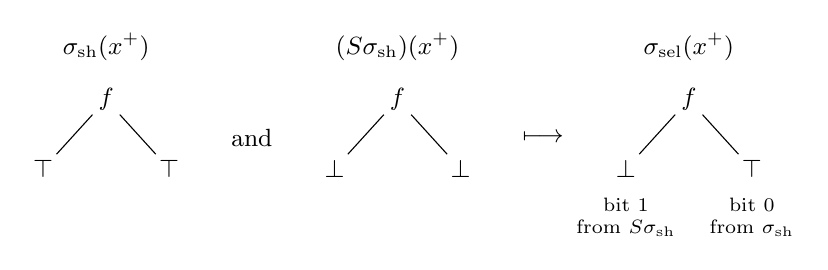
\begin{tikzpicture}[x=10mm,y=8mm,
    every node/.style={font=\small,inner sep=2pt}]
  \foreach \name/\pos/\leftlab/\rightlab in
    {h/0/\Top/\Top,d/3.7/\Bot/\Bot,s/7.4/\Bot/\Top} {
    \node (\name) at (\pos,0) {$f$};
    \node (\name0) at (\pos-0.8,-1.1) {$\leftlab$};
    \node (\name1) at (\pos+0.8,-1.1) {$\rightlab$};
    \draw (\name) -- (\name0);
    \draw (\name) -- (\name1);
  }
  \node[above=2mm of h] {$\sigma_{\mathrm{sh}}(x^+)$};
  \node[above=2mm of d] {$(S\sigma_{\mathrm{sh}})(x^+)$};
  \node[above=2mm of s] {$\sigma_{\mathrm{sel}}(x^+)$};
  \node at (1.85,-0.6) {and};
  \node at (5.55,-0.6) {$\longmapsto$};
  \node[below=1mm of s0,font=\scriptsize,align=center]
    {bit $1$\\from $S\sigma_{\mathrm{sh}}$};
  \node[below=1mm of s1,font=\scriptsize,align=center]
    {bit $0$\\from $\sigma_{\mathrm{sh}}$};
\end{tikzpicture}
\caption{Selection in \cref{ex:running-selection}. All three trees have the
same shape. At the positive root the choice bit is $0$; at children $0,1$
it is respectively $1,0$, yielding $f(\Bot,\Top)$.}
\Description{Three trees with a constructor root and two leaves. The least
shape has two top leaves, its image under the assignment involution has two bottom leaves, and the selected
tree takes the left bottom leaf from the dual and the right top leaf from the
least shape. The choice bits are one at the left child and zero at the right.}
\label{fig:polarity-selection}
\end{figure}


\subsection{The Four-Spine Extension}\label{sec:spine}
Throughout \cref{sec:spine,sec:bridge-formula,sec:events}, $\psi$ may be any
flip-closed, sign-coherent system on a signed variable set, and $x^+,y^+$
any two positive variables, with $x^-=\flip x^+$ and $y^-=\flip y^+$.
In particular, this includes both sides of \cref{sec:fixed-witness}: the
left side is $\phi^{\pm}$ with the roots $(x^+,y^+)$, and the right side is
$\phi^{\pm}$ under the complementary sign map, for which its roots
$(X_{\mathsf r},Y_{\mathsf r})=(y^-,x^-)$ are positive. The assignment
involution $S$, and hence the notion of a fixed solution, depends only on
the variable flip and is the same for both sign maps.

Fix $w=w[0]\cdots w[m-1]$ and $p_j=p(w[:j])$.
To enforce the two fixed-witness conditions and their sign duals, we seek
\begin{equation}\label{eq:g29}
\begin{aligned}
 \emb_\bot(w,\top)&\le\sigma(x^+),&
 \sigma(x^-)&\le\emb_\top(w,\bot),\\
 \sigma(y^+)&\le\emb_\top(w,f(\top)_i),&
 \emb_\bot(w,f(\bot)_i)&\le\sigma(y^-).
\end{aligned}
\end{equation}
The four families flatten these bounds along $w$:
\begin{center}
\small
\begin{tabular}{@{}llll@{}}
\toprule
Spine & Bound direction & Intended condition along $w$ & Sign-dual partner\\
\midrule
$P$ & lower & $x^+$ has a top prefix & $Q$\\
$Q$ & upper & $x^-$ has a bottom prefix & $P$\\
$Y$ & upper & $y^+$ has no top prefix & $W$\\
$W$ & lower & $y^-$ has no bottom prefix & $Y$\\
\bottomrule
\end{tabular}
\end{center}
The families $P$ and $Q$ start at the two signed copies $x^+$ and $x^-$
of the query root $x$, and $Y$ and $W$ at $y^+$ and $y^-$. Thus $Q$ and
$W$ are the sign duals of $P$ and $Y$: flipping signs exchanges $P$ with
$Q$ and $Y$ with $W$.
The spines $P$ and $Y$ express the fixed-witness conditions. Their
sign-dual partners make the extension flip-closed, so selection yields a
fixed solution.

Set
$P_0=x^+$, $Q_0=x^-$, $Y_0=y^+$, $W_0=y^-$.
For $1\le j\le m$ introduce fresh base variables $x_j,y_j$, which carry the
spines of $x$ and $y$ at cut $j$, and name
\[
 P_j=x_j^{p_j},\quad Q_j=x_j^{1\oplus p_j},\qquad
 Y_j=y_j^{p_j},\quad W_j=y_j^{1\oplus p_j}.
\]
Two further base variables $o_0,o_1$, for the off-path fillers, supply four
signed fillers
$B^0=o_0^0$, $T^1=o_0^1$, $T^0=o_1^0$, $B^1=o_1^1$.
Thus $\flip B^q=T^{1-q}$, $\flip P_j=Q_j$, and $\flip Y_j=W_j$.
The variables with positive index and the fillers are fresh. The cut-zero
names $P_0=x^+$, $Q_0=x^-$, $Y_0=y^+$, $W_0=y^-$ are old variables;
$P_0=Y_0$ and $Q_0=W_0$ when $x=y$.
There are $2k+4m+4$ signed variables.
For $R\in\{P,W\}$ and $Z\in\{Q,Y\}$ put
\[
 a^{R,j}_i=\begin{cases}R_{j+1}&i=w[j],\\B^{\operatorname{sg}(R_j)\oplus c(i)}&i\ne w[j],\end{cases}
 \qquad
 b^{Z,j}_i=\begin{cases}Z_{j+1}&i=w[j],\\T^{\operatorname{sg}(Z_j)\oplus c(i)}&i\ne w[j].\end{cases}
\]
The extension $\Psi^4_w$ consists of $\psi$ and
\begin{equation}\label{eq:g28}
\begin{array}{ll}
 f(a^{P,j}_i)_i\le P_j,&f(a^{W,j}_i)_i\le W_j\quad(0\le j<m),\\
 Q_j\le f(b^{Q,j}_i)_i,&Y_j\le f(b^{Y,j}_i)_i\quad(0\le j<m),\\
 P_m=\top,&Q_m=\bot,\\
 Y_m\le f(T^{p_m\oplus c(i)})_i,&f(B^{1\oplus p_m\oplus c(i)})_i\le W_m,\\
 B^q=\bot,&T^q=\top\quad(q=0,1).
\end{array}
\end{equation}
It is sign coherent: the distinguished child uses
$p_{j+1}=p_j\oplus c(w[j])$, and all other children, including terminal
children, have the prescribed sign by definition. It is flip-closed:
flip pairs the $P$ and $Q$ links, the $W$ and $Y$ links, the terminal
constants, the terminal constructor bounds, and the opposite-sign filler
constants. These identities also hold at cut zero and when $m=0$.

\Cref{fig:four-spines} displays the four parallel families of bounds;
the arrows indicate the distinguished child, not closure pairs.
\begin{figure}[t]
\centering
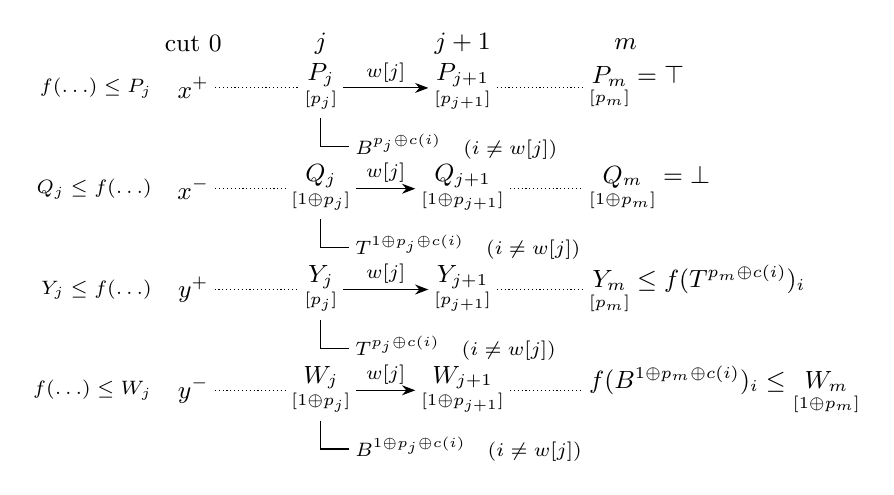
\begin{tikzpicture}[x=9mm,y=8mm,>=Stealth,
    every node/.style={font=\small,inner sep=2pt},
    filler/.style={font=\scriptsize,anchor=west}]
  \node[anchor=east,font=\scriptsize] at (-0.5,0) {$f(\ldots)\le P_j$};
  \node[anchor=east,font=\scriptsize] at (-0.5,-1.6) {$Q_j\le f(\ldots)$};
  \node[anchor=east,font=\scriptsize] at (-0.5,-3.2) {$Y_j\le f(\ldots)$};
  \node[anchor=east,font=\scriptsize] at (-0.5,-4.8) {$f(\ldots)\le W_j$};
  \node at (0,0.7) {cut $0$};
  \node at (1.8,0.7) {$j$};
  \node at (3.8,0.7) {$j+1$};
  \node at (6.1,0.7) {$m$};
  \foreach \spinerow/\spiney/\spineroot/\spinesign/\spinenextsign/\spinefiller in
    {P/0/x^+/p_j/p_{j+1}/B,
     Q/-1.6/x^-/1\oplus p_j/1\oplus p_{j+1}/T,
     Y/-3.2/y^+/p_j/p_{j+1}/T,
     W/-4.8/y^-/1\oplus p_j/1\oplus p_{j+1}/B} {
    \node (\spinerow0) at (0,\spiney) {$\spineroot$};
    \node (\spinerow j) at (1.8,\spiney) {$\underset{[\spinesign]}{\spinerow_j}$};
    \node (\spinerow next) at (3.8,\spiney) {$\underset{[\spinenextsign]}{\spinerow_{j+1}}$};
    \draw[densely dotted] (\spinerow0) -- (\spinerow j);
    \draw[->] (\spinerow j) -- node[above,font=\scriptsize] {$w[j]$} (\spinerow next);
    \draw (\spinerow j.south) -- ++(0,-0.45) -- ++(0.4,0)
      node[filler] {$\spinefiller^{\spinesign\oplus c(i)}\quad(i\ne w[j])$};
  }
  \node[anchor=west] (Pm) at (5.5,0) {$\underset{[p_m]}{P_m}=\Top$};
  \node[anchor=west] (Qm) at (5.5,-1.6) {$\underset{[1\oplus p_m]}{Q_m}=\Bot$};
  \node[anchor=west] (Ym) at (5.5,-3.2)
    {$\underset{[p_m]}{Y_m}\le f(T^{p_m\oplus c(i)})_i$};
  \node[anchor=west] (Wm) at (5.5,-4.8)
    {$f(B^{1\oplus p_m\oplus c(i)})_i\le\underset{[1\oplus p_m]}{W_m}$};
  \foreach \spinerow in {P,Q,Y,W} {\draw[densely dotted] (\spinerow next) -- (\spinerow m);}
\end{tikzpicture}
\caption{The four-spine extension along $w$, with $Q_j=\flip P_j$ and
$W_j=\flip Y_j$. Brackets give node signs; the root signs are $0,1,0,1$.
Each arrow reads the child $w[j]$. The $P,W$ links are lower constructor
bounds, and the $Q,Y$ links are upper bounds, with the displayed off-path
fillers. Dots abbreviate the other cuts. \Cref{ex:running-spines}
instantiates the construction at $w=0$.}
\Description{Four horizontal rows P, Q, Y, W run from their signed query
roots through cuts j and j plus one to cut m. Every step reads the letter at position j and
toggles the sign by its variance. P and W have bottom off-path fillers;
Q and Y have top fillers. The final P is top and Q is bottom. Y ends with
an upper constructor bound and W with a lower constructor bound.}
\label{fig:four-spines}
\end{figure}


\begin{example}[One contravariant step]\label{ex:running-spines}
For the running query and $w=0$, the root signs of $(P,Q,Y,W)$ are
$(0,1,0,1)$, and their signs at cut $1$ are $(1,0,1,0)$.
The new links and terminal bounds are exactly
\[
\begin{array}{ll}
 f(P_1,B^0)\le x^+,&x^-\le f(Q_1,T^1),\\
 y^+\le f(Y_1,T^0),&f(W_1,B^1)\le y^-,\\
 P_1=\Top,\quad Q_1=\Bot,&
 Y_1\le f(T^0,T^1),\quad f(B^1,B^0)\le W_1,
\end{array}
\]
together with $B^q=\Bot$ and $T^q=\Top$ for $q=0,1$.
Extend the fixed witness of \cref{ex:running-signed} by
\[
 \sigma(P_1)=\Top,\quad \sigma(Q_1)=\Bot,\qquad
 \sigma(Y_1)=f(\Top,\Top),\quad \sigma(W_1)=f(\Bot,\Bot).
\]
With the prescribed fillers this is a fixed solution of the extension,
which therefore has no label clash.
\end{example}

\begin{lemma}[Spine extension]\label{lem:spine}
An assignment $\sigma\models\psi$ extends to a solution of $\Psi^4_w$ iff
\begin{equation}\label{eq:g18}
\begin{array}{ll}
 \widehat{\sigma(x^+)}(w)=\top,&\widehat{\sigma(x^-)}(w)=\bot,\\
 \widehat{\sigma(y^+)}(w)\ne\top,&\widehat{\sigma(y^-)}(w)\ne\bot.
\end{array}
\end{equation}
\end{lemma}
\begin{proof}
Composing the links gives \eqref{eq:g29}.
The first bound forces a top at or before the final cut: an earlier bottom
violates the on-spine constructor bound, while reaching the end forces top.
Conversely, a top prefix satisfies the bound; all off-path bottom comparisons
are automatic. Duality proves the second equivalence. The third excludes
a top at every cut through the end, since the upper bound has constructors
there. A bottom ends comparison harmlessly; otherwise the terminal label
is at most $f$. Duality gives the fourth equivalence.
For sufficiency, assign, for each $1\le j\le m$,
\[
\begin{aligned}
\sigma(P_j)&=\emb_\bot(w[j:],\top),&
\sigma(Q_j)&=\emb_\top(w[j:],\bot),\\
\sigma(Y_j)&=\emb_\top(w[j:],f(\top)_i),&
\sigma(W_j)&=\emb_\bot(w[j:],f(\bot)_i).
\end{aligned}
\]
These are assignments to distinct fresh signed variables, so they impose
no extra condition on the old assignment, even when it is not fixed by
$S$. Assign each filler its prescribed constant.
For $m\ge1$, internal links and terminal literals hold with equality, and the root links
are the four bounds \eqref{eq:g29}; all newly assigned trees are finite,
so the extension stays in each of the three domains.
For $m=0$ the terminal literals themselves are those bounds at the old roots.
\end{proof}

\begin{theorem}[Four-spine unsafe-word criterion]\label{thm:four-spine}
On either side $\theta$, $w$ is $\theta$-unsafe iff the four-spine extension
of $\psi$ for the roots $(X_\theta,Y_\theta)$ has no label clash. No
satisfiability assumption is needed.
\end{theorem}
\begin{proof}
For the left side, an unsafe word gives a fixed witness by
\cref{lem:fixed-witness}. Fixedness supplies the opposite-sign conditions
in \eqref{eq:g18}, so \cref{lem:spine} extends it to a solution and excludes
a clash. Conversely, apply \cref{lem:selector} to the whole clash-free
extension \eqref{eq:g28}. The selected least shape is a fixed solution;
restriction to the old variables preserves satisfaction and fixedness,
and \cref{lem:spine} supplies all four prefix conditions. Its first and
third conditions give the fixed witness and hence unsafety.
For the right side, apply the same argument to $\psi$ with the roots
$(y^-,x^-)$, which are positive for the complementary sign map, and conclude
by \cref{lem:fixed-witness} for $\theta=\mathsf r$.
\end{proof}

\begin{lemma}[Separation]\label{lem:separation}
Partition the variables into old variables and the two fresh classes
\[
 \text{sources }\{P_j,W_j:1\le j\le m\}\cup\{B^0,B^1\},\qquad
 \text{sinks }\{Q_j,Y_j:1\le j\le m\}\cup\{T^0,T^1\}.
\]
Then

\begin{equation}\label{eq:g30}
\begin{array}{ll}
 D_{\Psi^4_w}(a,s),\ s\text{ a source}&\Longrightarrow a=s,\\
 D_{\Psi^4_w}(t,b),\ t\text{ a sink}&\Longrightarrow b=t,\\
 a,b\text{ old}:\quad D_{\Psi^4_w}(a,b)&\Longleftrightarrow D_\psi(a,b).
 \end{array}
\end{equation}

\end{lemma}

\begin{proof} Induct simultaneously on closure derivations.
An upper constructor literal has only old or sink children, never source
children; hence decomposition cannot have a source as its right endpoint.
Dually, a lower constructor literal has only old or source children, so
decomposition cannot have a sink as its left endpoint. This proves the
first two assertions, with transitivity collapsing the intervening identity.
For an old-to-old transitivity step, a fresh middle variable would be a source
or a sink and contradict these assertions. For an old-to-old decomposition
step, both bounding literals must be old: every new lower literal has only
source children, and every new upper literal has only sink children.
Apply induction to their old root pair. The other implication follows by
including the original derivation. Constants add no closure rule. \end{proof}

The classification here is by provenance of a literal, not the class of its
root: a new literal can be rooted at an old variable at cut zero.

\subsection{The Bridge Formula}\label{sec:bridge-formula}
Write $D=D_{\Psi^4_w}$ for the closure of the four-spine extension.
All path judgments in this subsection are in the base system $\psi$. Define

\begin{equation}\label{eq:g31}
U^R_j=\{v:\Up(w[:j],R_0,v)\},\qquad
 L^Z_j=\{v:\Lo(w[:j],v,Z_0)\},
\end{equation}

where $R\in\{P,W\}$ and $Z\in\{Q,Y\}$. Put $U_j=U^P_j$ and $L_j=L^Y_j$. By \eqref{eq:g25}, we have
$L^Q_j=\flip U_j$ and $U^W_j=\flip L_j$, where $\flip\mathcal U=\{\flip v:v\in\mathcal U\}$.
The sets $U^R_j$ are upward closed under $D_\psi$, and $L^Z_j$ are
downward closed. At cut zero,
$U^R_0=D_\psi\mathord\uparrow R_0$ and
$L^Z_0=D_\psi\mathord\downarrow Z_0$, where
$D_\psi\mathord\uparrow z=\{v:D_\psi(z,v)\}$ and
$D_\psi\mathord\downarrow z=\{v:D_\psi(v,z)\}$.

These sets already show why a clash can relate two different cuts. Take
cuts $s<e$ and $v\in U_e\cap L_s$. Where the subtrees exist, the path
bounds read
\[
 \sigma(x^+)|_{w[:e]}\le\sigma(v)\le\sigma(y^+)|_{w[:s]}.
\]
The upper embedding bound excludes a top leaf of $x^+$ before cut $e$.
If $x^+$ has a top leaf along $w$, its remaining path is therefore a
prefix of $w[e:]$, and the same bound forces a top prefix of $v$ there.
The lower embedding bound then forces a top leaf of
$y^+$ along $w[:s]w[e:]$. When $w[e:]\pre w[s:]$, this word is a prefix
of $w$, contradicting the target condition. The embedding formulation
handles an earlier top leaf of $y^+$ as well. In the extension, the old
variable $v$ links the $P$-spine at cut $e$ to the $Y$-spine at cut $s$,
and the equal suffixes carry this link down to the final cut. The bridge
formula describes all such links.

\begin{lemma}[Exact bridge formula]\label{lem:bridge}
For every old $v$, both lower names $R$, both upper names $Z$, and all $0\le j,j'\le m$,

\begin{equation}\label{eq:g32}
D_{\Psi^4_w}(R_j,v)\iff v\in U^R_j,
 \qquad D_{\Psi^4_w}(v,Z_{j'})\iff v\in L^Z_{j'},
\end{equation}

\begin{equation}\label{eq:g33}
\begin{split}
 D_{\Psi^4_w}(R_j,Z_{j'})\iff
 \exists \alpha\le j,\ \gamma\le j'\quad&
 U^R_\alpha\cap L^Z_\gamma\ne\varnothing,\\
 &j-\alpha=j'-\gamma,\qquad w[\alpha:j]=w[\gamma:j'].
 \end{split}
\end{equation}

\end{lemma}

The bridge consists of an old-variable intersection followed by parallel
descent through equal word factors (\cref{fig:bridge-descent}).
\begin{figure}[tbp]
\centering
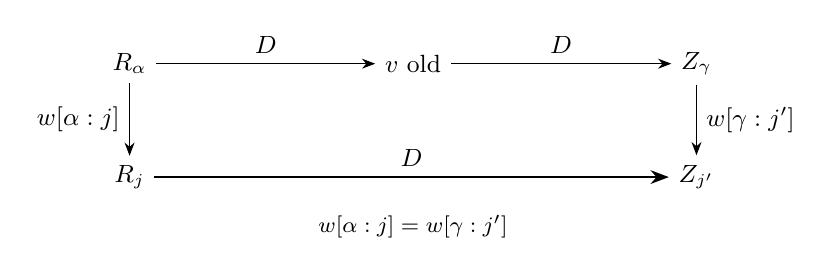
\begin{tikzpicture}[x=12mm,y=9mm,>=Stealth,every node/.style={font=\small}]
\node (ra) at (0,0) {$R_\alpha$};
\node (v) at (3,0) {$v$ old};
\node (zg) at (6,0) {$Z_\gamma$};
\node (rj) at (0,-1.6) {$R_j$};
\node (zj) at (6,-1.6) {$Z_{j'}$};
\draw[->] (ra) -- node[above] {$D$} (v);
\draw[->] (v) -- node[above] {$D$} (zg);
\draw[->] (ra) -- node[left] {$w[\alpha:j]$} (rj);
\draw[->] (zg) -- node[right] {$w[\gamma:j']$} (zj);
\draw[->,thick] (rj) -- node[above] {$D$} (zj);
\node[font=\footnotesize] at (3,-2.3) {$w[\alpha:j]=w[\gamma:j']$};
\end{tikzpicture}
\caption{A bridge in \cref{lem:bridge}. The old variable belongs to
$U^R_\alpha\cap L^Z_\gamma$. Horizontal arrows are closure pairs;
vertical arrows descend through distinguished children along the same
factor. Decomposition propagates the top-row pair $D(R_\alpha,Z_\gamma)$ to $D(R_j,Z_{j'})$.
The common factor may be empty.}
\Description{A lower spine root connects through an old variable to an
upper spine root. Parallel descent along equal factors yields a closure
pair between the two later spine nodes.}
\label{fig:bridge-descent}
\end{figure}


\begin{proof}\emph{Right to left.} At zero, \eqref{eq:g32} follows from \cref{lem:separation}. Factor
an upper path along $w[:j]$ at its last letter. By induction the upper path along $w[:j-1]$
gives a closure pair from $R_{j-1}$ to the root of an old upper literal;
decompose against the $R$-link at position $w[j-1]$, then use the
terminal closure of the path judgment. This gives the right-to-left direction
of the first equivalence in \eqref{eq:g32}. The lower-path argument with a $Z$-link proves the second.
For \eqref{eq:g33}, choose $v\in U^R_\alpha\cap L^Z_\gamma$. By \eqref{eq:g32}, we have
$D(R_\alpha,v)$ and $D(v,Z_\gamma)$. Their composite is $D(R_\alpha,Z_\gamma)$.
Decompose the two spine links successively along the common factor
$w[\alpha:j]=w[\gamma:j']$. This gives $D(R_j,Z_{j'})$.

\emph{Left to right.} Strengthen the induction on a closure
derivation to four simultaneous obligations: old-to-old reflection in \eqref{eq:g30},
the two implications \eqref{eq:g32} for each lower or upper name at positive indices,
and \eqref{eq:g33} for each of the four name pairs when both indices are
positive. Pairs with a bottom filler on the left or a top filler on the
right carry no additional obligation; such pairs can occur.

For transitivity, an intermediate source forces its incoming pair to
be an identity, and an intermediate sink forces its outgoing pair to be
an identity, by \eqref{eq:g30}. An old intermediate variable joins the
two path memberships, producing the intersection in \eqref{eq:g33}.
Decomposition advances both spines along the same letter; empty factors
retain closure, so the invariant also covers cut-zero aliases.
The remaining rule cases and zero endpoints are detailed in
\cref{app:spine-proofs}.
\end{proof}

\subsection{Exact Clash Analysis}\label{sec:events}
Let $\mathsf{Bot}=\{v:v=\bot\in\psi\}$ and
$\mathsf{Top}=\{v:v=\top\in\psi\}$. Define

\begin{equation}\label{eq:g34}
\begin{aligned}
 \operatorname{bot}(U)&\iff U\cap\mathsf{Bot}\ne\varnothing,\\
 \operatorname{top}(L)&\iff L\cap\mathsf{Top}\ne\varnothing,\\
 \operatorname{refl}(U,L)&\iff U\cap L\ne\varnothing,\\
 \ready(U,L)&\iff
 \operatorname{bot}(U)\lor\operatorname{top}(L)\lor
 \operatorname{refl}(U,L),\\
 \childtest(U)&\iff
 \exists v\in U,\vec b\quad v\le f(\vec b)\in\psi.
 \end{aligned}
\end{equation}

At cut $j$, bot-readiness bounds $x^+$ by bottom along $w[:j]$,
excluding a top prefix along $w$. Top-readiness forces a top prefix of
$y^+$ by cut $j$. Reflexivity readiness bounds $x^+$ by $y^+$ at the
same cut, so any remaining top prefix transfers to $y^+$.
These readings use the embedding bounds \eqref{eq:g23}, and thus also
cover trees that terminate before the cut. The child test at the terminal
cut bounds $x^+$ by a constructor along all of $w$, excluding a top
prefix there. It does not depend on a next letter: it asks only whether
$U$ contains the root of an upper constructor bound.

The two-cut events concern the following pairs of cuts.

\begin{definition}[Comparison]\label{def:comparison}
A \emph{comparison} of a word $w$ of length $m$ is a pair of cuts $(s,e)$
satisfying
\begin{equation}\label{eq:g35}
0\le s<e\le m,\qquad w[e:]\preceq w[s:].
\end{equation}
Its \emph{period} is $\varpi=e-s$, and its \emph{root} is the factor
$w[s:e]$. A comparison is \emph{terminal} if $e=m$.
\end{definition}

\Cref{sec:holes} interprets comparisons as periodic suffixes and gives
examples. A comparison of $w$ is \emph{cross-admitted} if
$L_s\cap U_e\ne\varnothing$, and \emph{self-admitted}
if $U_s\cap\flip U_e\ne\varnothing$.

\begin{theorem}[Exact clash analysis]\label{thm:clashes}
For either side, the four-spine extension $\Psi^4_w$ has a label
clash iff $\psi$ has a label clash or at least one of the
following events occurs:

\begin{equation}\label{eq:g36}
\begin{array}{ll}
 \text{(a)}&\exists j\le m\quad\ready(U_j,L_j),\\
 \text{(b)}&\childtest(U_m),\\
 \text{(c)}&\exists s<e\le m\quad w[e:]\preceq w[s:]\ \land\
 [L_s\cap U_e\ne\varnothing\ \lor\ U_s\cap\flip U_e\ne\varnothing].
 \end{array}
\end{equation}

\end{theorem}

Readiness (a) rules out a fixed witness at a single cut, and the child event
(b) rules it out at the final cut. A cross event in (c) transfers a top
prefix from $x^+$ to $y^+$ across two cuts. A self event makes
the top-prefix requirement on $x^+$ incompatible with the bottom-prefix
requirement on $x^-$.

\begin{center}
\small
\begin{tabular}{@{}lcccc@{}}
\toprule
Lower bound $\backslash$ upper bound & old & $Q_{j'}$ & $Y_{j'}$ & $B^q$\\
\midrule
old & inherited clash & bot / child & top & impossible\\
$P_j$ & bot / child & self & refl / cross & impossible\\
$W_j$ & top & refl / cross & none ($f/f$) & impossible\\
$T^q$ & impossible & impossible & impossible & impossible\\
\bottomrule
\end{tabular}
\end{center}
The entries classify incompatible labels only; a closure pair between
compatible constructor labels is not a clash. Here bot, top, and refl
are the three readiness kinds, and child is the terminal event.

\begin{proof}Suppose first that a clash occurs. Express the clash by its two
bounding literals and a closure pair between their roots. The only relevant
new lower bounds are the $P_j$-bounds, with label $f$ for $j<m$
and $\top$ for $j=m$, the $W_j$-bounds, all labeled $f$ (including $j=m$), and the bounds $T^q=\top$. The relevant new
upper bounds are the $Q_{j'}$-bounds, labeled $f$ for $j'<m$ and
$\bot$ for $j'=m$, the $Y_{j'}$-bounds, all labeled $f$, and
$B^q=\bot$. The fillers cannot participate: a pair out of $T^q$, or into
$B^q$, is an identity by \eqref{eq:g30}, and neither has an opposite incompatible
bound. Classify the remaining bounds by whether their literals belong to
$\psi$ or were added in \eqref{eq:g28}.

If both are old, separation gives an inherited clash in $\psi$. If the lower bound is a $P_j$-bound and the upper bound
is old, an upper bottom yields $\operatorname{bot}(U_j)$ by \eqref{eq:g32}.
An upper constructor clashes only against $P_m=\top$, and yields
$\childtest(U_m)$.

The remaining old/new cases are their sign duals or give top-readiness; see \cref{app:spine-proofs}.

For a new $P$-bound against a new $Y$-bound, the $Y$-bound has label $f$,
so the lower endpoint must be $P_m$. Apply \eqref{eq:g33} to $D(P_m,Y_{j'})$. Its cuts satisfy
$m-\alpha=j'-\gamma$, so $\alpha\ge \gamma$. If $\alpha=\gamma$, the intersection
$U_\alpha\cap L_\alpha$ gives reflexivity readiness. If $\alpha>\gamma$, set
$s=\gamma,e=\alpha$. The factor equality reads
$w[e:m]=w[s:s+m-e]$; this is exactly \eqref{eq:g35}, and the intersection is
the cross admission $L_s\cap U_e\ne\varnothing$.

The $W$/$Q$ case is the sign dual of this cross case; $W$/$Y$ labels are compatible.

For a $P$-bound against a $Q$-bound, at least one endpoint is terminal:
$j=m$ or $j'=m$. The cuts $\alpha,\gamma$ given by \eqref{eq:g33} have
$U_\alpha\cap\flip U_\gamma\ne\varnothing$. Purity excludes $\alpha=\gamma$, since
$U_\alpha$ and $\flip U_\alpha$ have opposite signs. If $\alpha<\gamma$, the equation
$j-\alpha=j'-\gamma$ forces $j'>j$, hence $j'=m$; set $s=\alpha,e=\gamma$.
If $\alpha>\gamma$, it forces $j>j'$, hence $j=m$; set $s=\gamma,e=\alpha$ and
replace a common element $v$ by $\flip v$. In both cases the
equal factors give \eqref{eq:g35} and the intersection is
$U_s\cap\flip U_e\ne\varnothing$. These two orientations are both
needed. All other new/new pairs either have equal constructor labels or
cannot supply a lower and an upper incompatible label. This exhausts the
clashes, including literals rooted at old variables when $m=0$.

Conversely, an inherited clash persists. Readiness and child events
produce the clashes in the table, as detailed in \cref{app:spine-proofs}.
For a cross admission choose $v\in U_e\cap L_s$. The bridge yields
$D(P_e,Y_s)$. By \eqref{eq:g35}, descend $m-e$ matching letters to obtain
$D(P_m,Y_{s+m-e})$, a top/constructor clash with $P_m=\top$. For a self admission
choose $v\in U_s\cap\flip U_e=U_s\cap L^Q_e$. Descend from
$D(P_s,Q_e)$ to $D(P_{s+m-e},Q_m)$. Since $s<e$, the left index
is strictly less than $m$, so this is a constructor/bottom clash.
When $e=m$, no descent is needed, and the same clashes remain valid. \end{proof}

\begin{remark}[Special cases of the clash analysis]\label{rem:clash-cases}
\leavevmode
\begin{itemize}[leftmargin=*]
\item For satisfiable $\psi$, inherited clashes are absent, so the events
  (a)--(c) are exactly the extension clashes.
\item Purity shows that a self-admitted comparison must have
  $p(w[s:e])=1$: its two upper sets must have opposite signs. Thus
  self-admissions disappear in the fully covariant case, but cannot be
  discarded for general variance.
\item When $x=y$, reflexivity puts $x^+$ in $U_0\cap L_0$, so readiness at
  zero excludes every unsafe word.
\item When $m=0$, only readiness and the terminal child test remain; the
  zero-cut bridge formulas cover all aliases.
\item At arity zero, the constructor $f()$ still supplies a genuine
  terminal bound and is detected by the child test.
\item Child is tested only at the terminal cut; readiness is tested at
  every cut, including zero and the terminal cut.
\end{itemize}
\end{remark}

\begin{example}[A cross event]\label{ex:cross-event}
Replace the running system by $\phi=\{x\le f(a,y),\ y\le f(a,b)\}$,
keeping $c=(1,0)$ and the query $x\le y$. Its signed literals with positive
roots are $x^+\le f(a^-,y^+)$ and $y^+\le f(a^-,b^+)$; the other two are
their sign duals, and the closure is the identity. Along $w=11$, the upper sets are $\{x^+\},\{y^+\},\{b^+\}$ and
the lower sets are $\{y^+\},\varnothing,\varnothing$. No cut is ready, the
terminal child test fails, and there is no self event. The only event is
the comparison $(0,1)$, with $w[1:]=1\pre11=w[0:]$, which is cross-admitted
because $y^+\in U_1\cap L_0$. \Cref{fig:cross-event} shows the resulting
clash. The shared variable $y^+$ supplies the bridge $D(P_1,Y_0)$ between
two different cuts, and the matching suffix transports it one letter down
to $D(P_2,Y_1)$, where $P_2=\top$ meets the upper constructor bound of $Y_1$.
\end{example}
\begin{figure}[t]
\centering
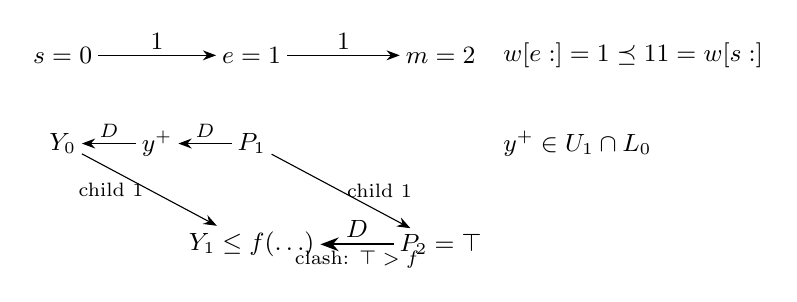
\begin{tikzpicture}[x=12mm,y=8mm,>=Stealth,
    every node/.style={font=\small,inner sep=2pt}]
  \node (s) at (0,0) {$s=0$};
  \node (e) at (2,0) {$e=1$};
  \node (m) at (4,0) {$m=2$};
  \draw[->] (s) -- node[above] {$1$} (e);
  \draw[->] (e) -- node[above] {$1$} (m);
  \node[anchor=west] at (4.6,0) {$w[e:]=1\pre 11=w[s:]$};
  \node (p1) at (2,-1.4) {$P_1$};
  \node (bridge) at (1,-1.4) {$y^+$};
  \node (y0) at (0,-1.4) {$Y_0$};
  \draw[->] (p1) -- node[above,font=\scriptsize] {$D$} (bridge);
  \draw[->] (bridge) -- node[above,font=\scriptsize] {$D$} (y0);
  \node[anchor=west] at (4.6,-1.4) {$y^+\in U_1\cap L_0$};
  \node (p2) at (4,-3) {$P_2=\Top$};
  \node (y1) at (2,-3) {$Y_1\le f(\ldots)$};
  \draw[->] (p1) -- node[right,font=\scriptsize] {child $1$} (p2);
  \draw[->] (y0) -- node[left,font=\scriptsize] {child $1$} (y1);
  \draw[->,thick] (p2) -- node[above] {$D$}
    node[below,font=\scriptsize] {clash: $\Top>f$} (y1);
\end{tikzpicture}
\caption{The nonterminal cross event of \cref{ex:cross-event}, for
$\phi=\{x\le f(a,y),\ y\le f(a,b)\}$ with $c=(1,0)$, the query $x\le y$,
and $w=11$. The comparison $(0,1)$ is cross-admitted through
$y^+\in U_1\cap L_0$. The bridge $D(P_1,Y_0)$ descends one matching letter to
$D(P_2,Y_1)$, where top meets an upper constructor bound.}
\Description{The word consisting of two ones has cuts zero, one and two,
with its one-letter suffix at cut one matching the prefix at cut zero.
A middle row connects P one through the shared variable y positive to Y zero.
Descending child one on both sides gives a closure pair from P two, labeled
top, to Y one, bounded above by a constructor. These labels clash.}
\label{fig:cross-event}
\end{figure}


\begin{example}[A self event]\label{ex:self-event}
Keep the arrow variance $c=(1,0)$ and take $\phi=\{x\le f(x,b)\}$, that is,
$x\le x\to b$, with the query $x\le y$ and $y$ unconstrained. The signed
literals are $x^+\le f(x^-,b^+)$ and $f(x^+,b^-)\le x^-$, and the closure is
the identity. Along $w=0$, the upper sets are $U_0=\{x^+\}$ and
$U_1=\{x^-\}$, and the lower sets are $L_0=\{y^+\}$ and $L_1=\varnothing$.
There are no constant literals and $U_j\cap L_j=\varnothing$, so neither cut
is ready, and $\childtest(U_1)$ fails because $x^-$ roots no upper constructor
bound. The terminal comparison $(0,1)$ is not cross-admitted, since
$L_0\cap U_1=\varnothing$, but it is self-admitted:
$U_0\cap\flip U_1=\{x^+\}$. The self event alone shows that $w=0$ is not
left unsafe. Semantically, $x\le_c x\to b$ excludes $x=\top$, so a top prefix
of $x^+$ along $0$ needs a bottom domain leaf, $x=f(\bot,t)$; but then
$x\le_c x\to b$ forces $x\le_c\bot$, which is impossible.
In the extension, $P_0=x^+$, $Q_0=x^-$, $P_1=\top$, and $Q_1=\bot$, with the
new links $f(P_1,B^0)\le x^+$ and $x^-\le f(Q_1,T^1)$. Decomposing the old
lower literal $f(x^+,b^-)\le x^-$ against the new upper link gives
$D(P_0,Q_1)$, and the new lower constructor bound on $P_0$ clashes with
$Q_1=\bot$. This is the terminal self case of \cref{thm:clashes}.
\end{example}

\section{Label Readers and Holes}
\label{sec:holes}

The clash tests now become a finite reader: rejection rules out the
single-cut events, while admission records the two-cut events. We show that
the resulting readers have the rejected-path property, which is the only
subtype-specific input to the word bounds.

\subsection{Words, Cuts, and Comparisons}

We use the word and cut notation of \cref{sec:words}; put $m=|w|$. Recall
from \cref{def:comparison} that a comparison of $w$ is a pair of cuts $s<e$
with $\wsuf{w}{e}\pre\wsuf{w}{s}$; its period is $\varpi=e-s$, its root is
$\wsub{w}{s}{e}$, and it is terminal when $e=m$. Comparisons are what the
readers below test.

Equivalently, $(s,e)$ is a comparison iff the suffix $\wsuf{w}{s}$ has period~$\varpi$, \ie
$w[i] = w[i-\varpi]$ for all $e \le i < m$, iff $\wsuf{w}{s}$ is a prefix of a power of its
root (\cref{lem:periodic}). Every pair $(s,m)$ is a terminal comparison. Over $\{0,1\}$, the
nonterminal comparisons of $w = 0100$ are $(0,3)$, because $\wsuf{w}{3} = 0$ is a prefix of
$w$, which has period~$3$, and $(2,3)$, because $0 \pre 00 = \wsuf{w}{2}$; the pair $(0,2)$ is
not a comparison, because $00$ is not a prefix of $0100$. Comparisons are inherited by
prefixes: if $(s,e)$ is a comparison of $w$ and $e \le h \le m$, then $(s,e)$ is a
comparison of $\wpre{w}{h}$. Extending a word may destroy a comparison when a new letter breaks its
period, and may create comparisons that end at the new cuts.


\begin{definition}[Reader hole]\label{def:reader-hole}
A \emph{reader} $(\mathcal{M},\Adm,\Rej)$ consists of a deterministic finite automaton
$\mathcal{M} = (Q,q_0,\delta)$ over a finite alphabet $\Gamma$, with transition function
$\delta : Q \times \Gamma \to Q$ extended to words by $\delta(q,\eps) = q$ and
$\delta(q,wa) = \delta(\delta(q,w),a)$, together with a relation $\Adm \subseteq Q \times Q$,
the \emph{admission relation}, and a set $\Rej \subseteq Q$ of \emph{rejected} states. A
state is \emph{reachable} if it is $\delta(q_0,w)$ for some word $w$. For a word $w$, write
$q_i = \delta(q_0,\wpre{w}{i})$ for the state at cut $i$. A word $w$ is a \emph{hole} of
$(\mathcal{M},\Adm,\Rej)$ if $q_{\len{w}} \in \Rej$ and no comparison $(s,e)$ of $w$ satisfies
$\Adm(q_s,q_e)$. States outside $\Rej$ are accepted.
\end{definition}
Rejection identifies a candidate counterexample word. An admitted comparison
disqualifies that candidate. Thus a hole requires both a rejected final state and the
absence of every admitted comparison.



\subsection{The Label Reader}\label{sec:label-reader}
For a set of signed variables define its one-letter updates

\begin{equation}\label{eq:g37}
\begin{aligned}
 E_i(U)&=\{v:\exists u\in U\quad\Up(i,u,v)\},\\
 G_i(L)&=\{v:\exists u\in L\quad\Lo(i,v,u)\}.
 \end{aligned}
\end{equation}

For a flip-closed, sign-coherent system $\psi$ and positive query roots
$x^+,y^+$, the \emph{label reader} has states $(U,L,b)$, where $U,L\subseteq V^{\pm}$
and $b\in\{0,1\}$. Its initial state and transition are

\begin{equation}\label{eq:g38}
q_0=(D_\psi\mathord\uparrow x^+,D_\psi\mathord\downarrow y^+,0),
 \qquad
 \delta_i(U,L,b)=(E_iU,G_iL,b\lor\ready(U,L)).
\end{equation}

The bit $b$ is a \emph{latch}: once set, it stays set and records readiness
at an earlier cut. It is needed because readiness at any earlier cut
excludes every extension from being unsafe, even if readiness later disappears.
Since $|V^\pm|=2k$, each of $U,L$ has $2^{2k}$ possible values;
together with the two latch values this gives
$2\cdot2^{2k}\cdot2^{2k}=2\cdot4^{2k}$ states.
All transitions and tests are computable
from the finite closure. Write $q_j$ for the state after $w[:j]$.
The path rules (\cref{lem:path-rules}) and induction on $j$ prove the run invariant

\begin{equation}\label{eq:g39}
q_j=(U_j,L_j,b_j),\qquad
 b_j=1\iff\exists h<j\quad\ready(U_h,L_h).
\end{equation}

Designate as rejected the states

\begin{equation}\label{eq:g40}
\Rej=\{(U,L,b):b=0\land\neg\ready(U,L)
                         \land\neg\childtest(U)\},
\end{equation}

and define the binary state relation

\begin{equation}\label{eq:g41}
\Adm((U,L,b),(U',L',b'))
 \iff L\cap U'\ne\varnothing\ \lor\ U\cap\flip U'\ne\varnothing.
\end{equation}

A word $w$ is a hole precisely when
\begin{equation}\label{eq:g42}
q_m\in \Rej\quad\land\quad
 \forall s<e\le m,\quad w[e:]\preceq w[s:]\Longrightarrow\neg \Adm(q_s,q_e).
\end{equation}
The set of holes of a reader need not be a regular language, even for a
label reader, since the comparison test relates suffixes that start at
different cuts; \cref{sec:general-holes} gives an example. The argument
does not require regularity.

There is one reader construction, with two instances: the \emph{left and
right label readers}. The left label
reader uses $\psi$ with the roots $(x^+,y^+)$; the right one uses the same
system $\psi$ with the roots $(y^-,x^-)$, which are positive for the
complementary sign map (\cref{sec:spine}). Closure, path updates, readiness,
child, and admission are the same for both; only the initial state differs.
By \cref{lem:fixed-witness}, a top prefix of $y^-$ is a bottom prefix of
$y$, so the right label reader tests right unsafety.
Write $(\mathcal M_\theta,\Adm_\theta,\Rej_\theta)$ for the instance on
$\psi$ with the roots $(X_\theta,Y_\theta)$ defined in
\cref{sec:fixed-witness}.

\begin{example}[Reading the running query]\label{ex:running-reader}
We run the left-side construction on the signed system of
\cref{ex:running-signed} along $00$, for the failing query $x\le y$ and,
for contrast, for the entailed query $y\le x$, which exchanges the roots.
Neither half is the right label reader of $x\le y$, which would start
from the roots $(y^-,x^-)$. The last three columns give the latch, readiness,
and acceptance status at each cut, before the next letter is read.
\begin{center}
\small
\begin{tabular}{@{}ccccccl@{}}
\toprule
Query & cut $j$ & $U_j$ & $L_j$ & $b_j$ & $\ready$ & status\\
\midrule
$x\le y$ & $0$ & $\{x^+\}$ & $\{y^+\}$ & $0$ & false & accepted (child)\\
 & $1$ & $\{a^-\}$ & $\varnothing$ & $0$ & false & rejected\\
 & $2$ & $\varnothing$ & $\varnothing$ & $0$ & false & rejected\\
\midrule
$y\le x$ & $0$ & $\{y^+\}$ & $\{x^+\}$ & $0$ & false & accepted (child)\\
 & $1$ & $\{a^-\}$ & $\{a^-\}$ & $0$ & true & accepted (ready)\\
 & $2$ & $\varnothing$ & $\varnothing$ & $1$ & false & accepted (latch)\\
\bottomrule
\end{tabular}
\end{center}
For $x\le y$, the word $0$ is a hole: its final state is rejected,
and its only comparison $(0,1)$ is not admitted. The word $00$ is also
a hole. The empty word is accepted by the child test; it is not a
left-unsafe word. For the entailed reverse query, readiness at cut $1$
sets the latch at cut $2$, so the empty upper and lower sets there do
not cause rejection.

Rejection alone does not certify a hole. In the cross event of
\cref{ex:cross-event}, the run on $11$ has $b_j=0$ throughout and ends
in $(\{b^+\},\varnothing,0)$, a rejected state. Nevertheless $(0,1)$
is cross-admitted, so $11$ is not a hole.
\end{example}

\subsection{The Rejected-Path Property}\label{sec:interface}
For a general reader $(\mathcal{M},\Adm,\Rej)$, write $q_j=\delta(q_0,w[:j])$. If $q_m\in\Rej$,
let $J=J(w)$ be the least cut with $q_J\in\Rej$, and put $r(w)=|w|-J(w)$. The reader has the
\emph{rejected-path property} if it satisfies \emph{betweenness} and
the \emph{admission cone}:

\begin{description}[style=nextline,leftmargin=1em,font=\normalfont\itshape]\item[Betweenness] if two prefixes of a word end in $\Rej$, every intermediate
  prefix also ends in $\Rej$.
\item[Admission cone] in a word ending in $\Rej$, every comparison
  $(s,e)$ that satisfies $\Adm(q_s,q_e)$ has $e\le J$.

\end{description}

\begin{lemma}[Rejected paths of label readers]\label{lem:between}\label{lem:cone}
The label reader, and hence both the left and the right label reader, satisfies the rejected-path
property, without any satisfiability assumption.
\end{lemma}

\begin{proof} Rejection at a cut implies $\neg\childtest(U)$.
Every reachable $U$ is upward closed under $D_\psi$: this holds at
$q_0$ and is preserved by each $E_i$, using \eqref{eq:g22} and transitivity.
If $E_iU\ne\varnothing$, \eqref{eq:g22} supplies an upper constructor with root
$z$ reached from some $u\in U$. Upward closure puts $z\in U$,
giving $\childtest(U)$, a contradiction. Thus $U$ becomes
empty on the next letter and remains empty thereafter. Both disjuncts of \eqref{eq:g41} require a
nonempty upper set at their second cut. Any admission therefore has
$e\le J$, proving the admission cone.

For betweenness, after a rejected cut every later upper set is empty. A later
state can cease to be rejected only through readiness or an already set
latch; a child can no longer occur. Once readiness occurs, it is present
at that cut and sets the latch at the next one, making every subsequent
state accepted. Consequently it cannot occur between two rejected cuts.
This proves betweenness for either instance of the construction. \end{proof}

The proof gives more than the admission cone: it excludes later
admissions even for pairs that are not comparisons. The rejected-path property retains
only what the tail proof needs; this stronger restriction may help sharpen
subtype-specific bounds. Rejection need not be absorbing: a later ready
state can become accepted permanently.

\subsection{Unsafe Words and Holes}\label{sec:side-bridge}
\begin{theorem}[Unsafe words are holes]\label{thm:holes}
If $\Sat_c(\phi)$, then for either side $\theta$,

\begin{equation}\label{eq:g44}
w\text{ is }\theta\text{-unsafe}
 \quad\Longleftrightarrow\quad
 w\text{ is a hole of }(\mathcal{M}_\theta,\Adm_\theta,\Rej_\theta).
\end{equation}\end{theorem}

\begin{proof} By \cref{thm:four-spine}, unsafety is equivalent to absence
of a label clash in the side's four-spine extension. Satisfiability excludes
inherited clashes in $\psi$, so \cref{thm:clashes} identifies
this with the simultaneous negation of \eqref{eq:g36}.
The run and test formulas \eqref{eq:g39}--\eqref{eq:g41} identify those negations precisely
with \eqref{eq:g42}, using the right label reader for the right side. Every implication is reversible. The argument uses
no positive-arity assumption; the letter-free child test also handles the
empty word over the empty alphabet. \end{proof}

\subsection{Consequences for General Readers}
For any reader satisfying the rejected-path property, the following consequences hold.

\begin{corollary}[Hole criterion]\label{cor:normal}
A rejected word $w$ is a hole iff it has no admitted comparison $(s,e)$ with $e \le J(w)$.
\end{corollary}

\begin{lemma}[Rejected extension]\label{lem:extension}
If $v$ is a hole and $w$ is a rejected word with $v \pre w$, then $w$ is a hole.
\end{lemma}

\begin{proof}
Since $v$ is rejected, $J(w) = J(v) \le \len{v}$. An admitted comparison $(s,e)$ of $w$ has
$e \le J(w) \le \len{v}$ by the admission cone, so it is also a comparison of $v$, with the
same cut states. This contradicts the assumption that $v$ is a hole.
\end{proof}

\Cref{tab:reader-hypotheses} separates the subtype-specific rejected-path property
from the general word arguments.
\begin{table}[tbp]
\caption{Hypotheses used by the word bounds.}
\label{tab:reader-hypotheses}
\centering
\begin{tabular}{@{}p{.44\linewidth}p{.51\linewidth}@{}}
\toprule
Result & Hypotheses on the reader and word\\
\midrule
Rejected extension (\cref{lem:extension}) & Admission cone; a hole and a rejected extension\\
Bounded tail (\cref{thm:brt}) & Admission cone and betweenness; some hole\\
Return gap and depth (\cref{lem:return-gap,thm:depth}) & Any reader; a rejected word, nonempty for depth\\
Bounded-depth compression (\cref{thm:search}) & Any reader; a nonempty hole of bounded depth\\
\bottomrule
\end{tabular}
\end{table}

\begin{example}[Loop deletion can create an admission]\label{ex:loop-deletion}
Consider the reader on $\{0,1\}$ with initial state $q$, rejected set
$\Rej=\{r\}$, sole admitted pair $(q,b)$, and all transitions as follows:
\begin{center}
\begin{tabular}{@{}c|cccccc@{}}
state & $q$ & $a$ & $b$ & $c$ & $r$ & $h$\\
\hline
$0$ & $a$ & $a$ & $c$ & $h$ & $r$ & $h$\\
$1$ & $h$ & $b$ & $h$ & $r$ & $r$ & $h$
\end{tabular}
\end{center}
Here $h$ is an accepted sink. State $q$ occurs only at cut $0$, so a
comparison is admitted only if it starts at cut $0$ and ends at a cut in
state $b$. Deleting the loop $a\xrightarrow{0}a$ between the equal-state
cuts $1$ and $2$ of $00101$ gives $0101$; both runs end in the rejected
state $r$:
\[
\begin{array}{r@{\quad}l}
 00101: & q\xrightarrow{0}a\xrightarrow{0}a\xrightarrow{1}b
          \xrightarrow{0}c\xrightarrow{1}r,\\[2pt]
 0101: & q\xrightarrow{0}a\xrightarrow{1}b\xrightarrow{0}c\xrightarrow{1}r.
\end{array}
\]
In $00101$, state $b$ occurs only at cut $3$, so the only candidate is
$(0,3)$. It is not a comparison: the suffix $01$ at cut $3$ is not a
prefix of $00101$. Thus $00101$ is a hole. In $0101$, state $b$ occurs at
cut $2$, and the candidate $(0,2)$ is a comparison, since the suffix $01$
at cut $2$ is a prefix of $0101$. Its states are $(q,b)$, so it is
admitted, and the shortened word is not a hole.

This reader has the rejected-path property. State $r$ is absorbing,
which proves betweenness. Any admission must start at $q$ and end at
$b$; $q$ occurs only initially, and $b$ can occur only before the first
visit to $r$. Hence every admitted comparison of a rejected word ends
before $J$, proving the admission cone. This example motivates the
simultaneous comparison summaries in \cref{sec:search}.
\end{example}

\section{Bounded Rejected Tails}
\label{sec:tail}

The first bound selects a hole whose rejected tail is short. Throughout,
$(\mathcal M,\Adm,\Rej)$ is an $N$-state reader over a finite alphabet
$\Gamma$, with initial state $q_0$ and transition function $\delta$,
that has the rejected-path property (\cref{sec:interface}). By
\cref{lem:extension}, every rejected extension of a hole is a hole.

\begin{theorem}[Bounded rejected tail]\label{thm:brt}
Let $(\mathcal{M},\Adm,\Rej)$ be a reader over a finite alphabet with $N$ states that satisfies
betweenness and the admission cone. If it has a hole, then it has a hole $w$ whose rejected tail
satisfies $r(w) \le 4N - 2$.
\end{theorem}

The theorem \emph{selects} a hole. It bounds neither the tail of every
hole nor a continuation of each fixed first rejected prefix. The proof
may replace the prefix before the rejected tail.

\paragraph{The Rejected Graph}
Call a letter $i$ \emph{safe} at a state $q \in \Rej$ if $\delta(q,i) \in \Rej$. The
\emph{rejected graph} $G$ has as vertices the reachable states in $\Rej$ and an edge
$q \xrightarrow{i} \delta(q,i)$ for every safe letter. We count edges by letters, so a state
whose distinct letters lead to the same successor has separate outgoing edges. A vertex is
\emph{cyclic} if it lies on a cycle of~$G$. If the initial state is rejected, the empty
word is a hole with tail~$0$; we assume from now on that $q_0 \notin \Rej$. The proof
distinguishes whether some cyclic vertex has two safe letters.

\subsection{Branching Cycles}

Repeating a cycle sufficiently often and then choosing a different next
letter destroys every comparison whose right endpoint lies in the preceding
prefix.

\begin{lemma}[Rotation]\label{lem:rotation}
Let $v, \kappa \in \Gamma^*$ with $\len{v} = a$ and $\len{\kappa} = \nu \ge 1$, let the exponent
$\mu$ satisfy $\mu\nu \ge a + \nu$, and let $b \ne \kappa[0]$ be a letter. Then the word
$w = v\,\kappa^\mu\,b$ has no comparison $(s,e)$ with $e \le a$.
\end{lemma}

\begin{proof}
Let $(s,e)$ be a comparison with $e \le a$ and period $\varpi = e - s \le a$, so
$w[k] = w[k-\varpi]$ for $e \le k < \len{w}$. For the $\nu$ positions $k = a+\varpi, \dots, a+\varpi+\nu-1$,
both $k$ and $k-\varpi$ lie in the block $\kappa^\mu$, because $\varpi + \nu \le \mu\nu$. Writing
$i = (k-\varpi-a) \bmod \nu$, which ranges over all residues, we obtain $\kappa[(i+\varpi) \bmod \nu] = \kappa[i]$
for all $i$: the cyclic word $\kappa$ is invariant under rotation by $\varpi$. The last position
$k = a + \mu\nu$ also satisfies $k \ge e$ and $k - \varpi \ge a$, so
$w[k-\varpi] = \kappa[(\mu\nu-\varpi) \bmod \nu] = \kappa[(-\varpi) \bmod \nu]$, which equals $\kappa[0]$ by the rotation
invariance with $i = (-\varpi) \bmod \nu$. But $w[k] = b \ne \kappa[0]$.
\end{proof}

\begin{lemma}[Branching cycle]\label{lem:branching}
If some cyclic vertex of $G$ has two safe letters, the reader has a hole with tail at most
$4N - 2$.
\end{lemma}

\begin{proof}
Let $q$ be such a vertex, $v$ a shortest word with $\delta(q_0,v) = q$, so $a = \len{v} \le
N - 1$, and $\kappa$ the label of a simple cycle of $G$ through $q$, so $1 \le \nu = \len{\kappa}
\le N$. Let $b \ne \kappa[0]$ be another safe letter at $q$ and
$\mu = \lceil (a+\nu)/\nu \rceil$. The word $w = v\,\kappa^\mu\,b$ (\cref{fig:branching}) is rejected:
after $v$ it stays in $G$. Its first rejected cut satisfies $J \le a$, so by the admission cone every
admitted comparison has $e \le a$, and by \cref{lem:rotation} there is none. Thus $w$ is a
hole. Since $\mu\nu < a + 2\nu$, its tail is at most $\len{w} = a + \mu\nu + 1 \le 2a + 2\nu \le
4N - 2$.
\end{proof}

The lemma does not assume that a hole exists. For a satisfiable $\phi$, a reachable rejected cycle of its
label reader with a second safe letter therefore already refutes entailment.
For a fixed finite alphabet, reachability and cycle detection give a
sufficient test polynomial in the reader graph size, applicable to either
side at any variance.

\begin{figure}[t]
\centering
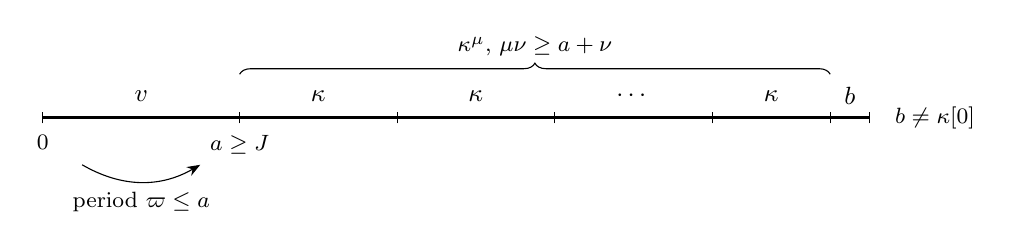
\begin{tikzpicture}[x=5mm,y=5mm,>=Stealth]
  \draw[thick] (0,0) -- (21,0);
  \foreach \x in {0,5,9,13,17,20,21} { \draw (\x,-0.15) -- (\x,0.15); }
  \node[font=\small] at (2.5,0.55) {$v$};
  \node[font=\small] at (7,0.55) {$\kappa$};
  \node[font=\small] at (11,0.55) {$\kappa$};
  \node[font=\small] at (15,0.55) {$\cdots$};
  \node[font=\small] at (18.5,0.55) {$\kappa$};
  \node[font=\small] at (20.5,0.55) {$b$};
  \node[below,font=\footnotesize] at (0,-0.2) {$0$};
  \node[below,font=\footnotesize] at (5,-0.2) {$a \ge J$};
  \draw[->] (1,-1.2) to[bend right=30] node[below,font=\footnotesize] {period $\varpi \le a$} (4,-1.2);
  \draw[decorate,decoration={brace,amplitude=4pt}] (5,1.1) -- (20,1.1)
    node[midway,above=3pt,font=\footnotesize] {$\kappa^\mu$, $\mu\nu \ge a+\nu$};
  \node[font=\footnotesize,align=left,anchor=west] at (21.4,0) {$b \ne \kappa[0]$};
\end{tikzpicture}
\caption{The branching case (\cref{lem:branching}). A period $\varpi \le a$ that survives the
block $\kappa^\mu$ makes $\kappa$ invariant under rotation by $\varpi$ and then predicts the letter $\kappa[0]$ at
the end, where the word has $b \ne \kappa[0]$.}
\Description{A word v followed by mu copies of a cycle word kappa and a final letter b different from the first letter of kappa.}
\label{fig:branching}
\end{figure}

\subsection{Forced Cycles}

In the remaining case, every cyclic vertex of $G$ has exactly one safe letter: at least one,
the next edge of its cycle, but not two. Then the path of $G$ from a cyclic
vertex is \emph{forced}: it follows the unique safe letter and returns to its start. We now
use the existence of a hole.

Let $w_0$ be a hole with first rejected cut $J_0$ and length $m_0$. If its tail is shorter
than $N$, we are done. Otherwise, the run of $w_0$ from cut $J_0$ to cut $m_0$ stays in
$G$ by betweenness and visits more than $N$ cuts, so it repeats a state; from
that point it is on a forced cycle, and so is its last state $q_{m_0}$. Extending $w_0$
along the forced cycle forever gives an infinite word $\Omega = w_0\,\kappa^\omega$, where $\kappa$ spells
the cycle from $q_{m_0}$. Every finite prefix of $\Omega$ of length at least $m_0$ is a
rejected extension of $w_0$, hence a hole. Write $\Omega[s{:}]$ for the infinite suffix from cut
$s$, and call a pair of cuts $s < e$ an \emph{equal-suffix pair} if $\Omega[s{:}] = \Omega[e{:}]$.

\begin{lemma}[No admitted equal-suffix pair]\label{lem:no-infinite}
$\Omega$ has no equal-suffix pair $(s,e)$ with $\Adm(q_s,q_e)$.
\end{lemma}

\begin{proof}
Such a pair is a comparison of every prefix of $\Omega$ of length at least $\max(m_0,e)$, with
the same cut states, and these prefixes are holes.
\end{proof}

Let $\nu \le N$ be the least period of $\kappa^\omega$, and let $A$ be the \emph{earliest
periodic onset}, the least cut from which $\Omega$ is $\nu$-periodic: $\Omega[k] = \Omega[k+\nu]$ for all
$k \ge A$. Then $A \le m_0$, and if $A > 0$, minimality gives
\begin{equation}\label{eq:onset}
  \Omega[A-1] \ne \Omega[A-1+\nu].
\end{equation}

\begin{lemma}[Earliest onset]\label{lem:onset}
Every equal-suffix pair $(s,e)$ of $\Omega$ has $s \ge A$.
\end{lemma}

\begin{proof}
Let $\varpi = e - s$. The equality $\Omega[s{:}] = \Omega[e{:}]$ gives $\Omega[k] = \Omega[k + j\varpi]$ for all
$k \ge s$ and $j \ge 0$. For $k \ge s$ and $j$ large enough that $k + j\varpi \ge A$, we get
$\Omega[k+\nu] = \Omega[k+\nu+j\varpi] = \Omega[k+j\varpi] = \Omega[k]$. So $\Omega$ is $\nu$-periodic from $s$, and $s \ge A$ by
minimality of~$A$.
\end{proof}

\paragraph{Compressing the Prefix}
The word $\Omega$ can be long before its periodic part; we replace that prefix by a shorter one. If
$A = 0$, let $u = \eps$. Otherwise, let $u = v'\,\Omega[A-1]$, where $v'$ is a shortest word with
$\delta(q_0,v') = q_{A-1}$; then $\len{u} \le N$ and $\delta(q_0,u) = q_A$. Let
$\Omega' = u\,\Omega[A{:}]$ (\cref{fig:forced}). The suffix of $\Omega'$ after cut $\len{u}$ is the suffix
of $\Omega$ after cut $A$, read from the same state, so cuts $\len{u}+k$ of $\Omega'$ and $A+k$ of
$\Omega$ carry the same states and the same suffixes. The letter before the onset is preserved,
so by \eqref{eq:onset} the earliest periodic onset of $\Omega'$ is exactly $\len{u}$.

\begin{lemma}[No admitted pair after compression]\label{lem:no-infinite-prime}
$\Omega'$ has no equal-suffix pair $(s,e)$ with $\Adm(q'_s,q'_e)$, where $q'_i$ are the cut
states of~$\Omega'$.
\end{lemma}

\begin{proof}
By \cref{lem:onset} applied to $\Omega'$, such a pair has $s \ge \len{u}$. It corresponds to the
pair $(s - \len{u} + A,\ e - \len{u} + A)$ of $\Omega$, with the same states and suffixes,
contradicting \cref{lem:no-infinite}.
\end{proof}

\paragraph{Rejection After the First Rejected Cut}
Cut $\len{u}+k$ of $\Omega'$ carries the state of cut $A+k$ of $\Omega$. Every cut of $\Omega$
from $m_0 \ge A$ on is rejected, so every cut of $\Omega'$ from $\len{u} + m_0 - A$ on is
rejected. Let $J'$ be the first rejected cut of $\Omega'$. Every later cut lies between $J'$
and a rejected cut further on, so by betweenness every cut of $\Omega'$ from $J'$ on is
rejected. The truncation therefore need not wait until $\Omega'$ returns to the original
state and phase of the cycle.

\begin{lemma}[Periodic truncation]\label{lem:truncation}
Let $J'$ be the first rejected cut of $\Omega'$ and $L = \len{u} + J' + \nu$. Then the prefix
$w' = \Omega'[{:}L]$ of length $L$ is a hole.
\end{lemma}

\begin{proof}
Since $L \ge J'$, the word $w'$ is rejected, and its first rejected cut is $J'$. Suppose
$(s,e)$ is an admitted comparison of $w'$. By the admission cone, $e \le J'$, so its period
satisfies $\varpi = e - s \le J'$, and $\Omega'[k] = \Omega'[k-\varpi]$ for $e \le k < L$. Put
$h = \max(e, \len{u}+\varpi)$. Since $e \le J'$ and $\varpi \le J'$, we have $h + \nu \le L$, so the
equality holds at the $\nu$ consecutive positions $k = h, \dots, h+\nu-1$. These satisfy
$k - \varpi \ge \len{u}$, so both $k$ and $k-\varpi$ lie in the $\nu$-periodic part of $\Omega'$.
Equality on $\nu$ consecutive positions of a $\nu$-periodic word propagates to all later
positions, so $\Omega'[k] = \Omega'[k-\varpi]$ for all $k \ge e$; that is, $(s,e)$ is an
equal-suffix pair of $\Omega'$ with $\Adm(q'_s,q'_e)$. This contradicts
\cref{lem:no-infinite-prime}.
\end{proof}

\begin{figure}[t]
\centering
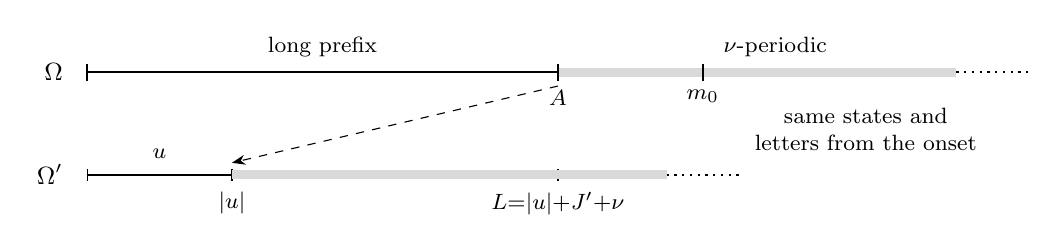
\begin{tikzpicture}[x=4.6mm,y=5mm,>=Stealth]
  % original infinite word \Omega
  \node[anchor=east,font=\small] at (-0.4,0) {$\Omega$};
  \draw[thick] (0,0) -- (24,0);
  \draw[thick,dotted] (24,0) -- (26,0);
  \fill[black!15] (13,-0.12) rectangle (24,0.12);
  \foreach \x in {0,13,17} { \draw[thick] (\x,-0.22) -- (\x,0.22); }
  \node[below,font=\footnotesize] at (13,-0.2) {$A$};
  \node[below,font=\footnotesize] at (17,-0.2) {$m_0$};
  \node[above,font=\footnotesize] at (6.5,0.15) {long prefix};
  \node[above,font=\footnotesize] at (19,0.15) {$\nu$-periodic};
  % compressed word \Omega'
  \node[anchor=east,font=\small] at (-0.4,-2.6) {$\Omega'$};
  \draw[thick] (0,-2.6) -- (16,-2.6);
  \draw[thick,dotted] (16,-2.6) -- (18,-2.6);
  \foreach \x in {0,4,13} { \draw (\x,-2.75) -- (\x,-2.45); }
  \fill[black!15] (4,-2.72) rectangle (16,-2.48);
  \node[above,font=\footnotesize] at (2,-2.45) {$u$};
  \node[below,font=\footnotesize] at (4,-2.8) {$\len{u}$};
  \node[below,font=\footnotesize] at (13,-2.8) {$L{=}\len{u}{+}J'{+}\nu$};
  \draw[->,dashed] (13,-0.35) -- (4,-2.3);
  \node[font=\footnotesize,align=center] at (21.5,-1.45) {same states and\\letters from the onset};
\end{tikzpicture}
\caption{The forced case. The prefix of $\Omega$ before the earliest periodic onset $A$ is
replaced, for $A>0$, by a shortest path to $q_{A-1}$ followed by the
original letter $\Omega[A-1]$; for $A=0$, the replacement prefix is empty.
Every cut of the resulting word $\Omega'$ from its first rejected cut $J'$ on is rejected,
and its prefix of length $L=\len{u}+J'+\nu$ is a hole.}
\Description{The infinite word Omega with a long prefix before the periodic onset A, and the compressed word Omega-prime with a short prefix u and the truncation cut L.}
\label{fig:forced}
\end{figure}

\begin{proof}[Proof of \cref{thm:brt}]
If the initial state is rejected, the empty word is a hole. If a cyclic vertex of $G$ has
two safe letters, \cref{lem:branching} gives a hole with tail at most $4N - 2$.
Otherwise, starting from any hole, either its tail is less than $N$, or
\cref{lem:truncation} gives a hole with tail $L - J' = \len{u} + \nu \le 2N$. Since $N \ge 1$,
all these bounds are at most $4N - 2$.
\end{proof}



The essential choice is the \emph{earliest}
periodic onset: preserving its preceding letter excludes equal-suffix
pairs starting in the replacement prefix. The admission cone reduces the
rest to the finite window of \cref{lem:truncation}, and betweenness lets
that window start right after the replacement prefix. If the alphabet is
empty, the only word is $\eps$.

\section{From Short Tails to Bounded Depth}
\label{sec:depth}

A hole with a short rejected tail can still be arbitrarily long. The second bound
measures its complexity by the depth of a canonical hierarchy of block decompositions, and
shows that this depth is bounded in terms of the tail. The hierarchy is the device that
makes comparisons tractable: each of its levels collects the starting points of the
comparisons that end at one particular cut.

\subsection{The Canonical Desubstitution Hierarchy}

Let $\Gamma$ be an alphabet and $u \in \Gamma^+$ a nonempty word with last letter $\ell$,
the \emph{marker}. Then $u$ factors uniquely as
\[
  u = X_0\,\ell\,X_1\,\ell \cdots X_{h-1}\,\ell \qquad\text{with } X_i \in (\Gamma\setminus\{\ell\})^*.
\]
The \emph{desubstitution} of $u$ is the word $[X_0][X_1]\cdots[X_{h-1}]$ of length $h$
over the alphabet of \emph{blocks} $(\Gamma\setminus\{\ell\})^*$: each block $[X_i]$, a word
over $\Gamma$, is a single letter of the new word. Expanding every block $[X]$ to $X\ell$
recovers~$u$. The
name follows the use of desubstitution and derived sequences in symbolic dynamics
\citep{Durand98}.

\begin{definition}[Hierarchy and depth]\label{def:hierarchy}
The \emph{canonical hierarchy} of a nonempty word $w$ is the sequence $u_0 = w$ and
$u_{j+1} = $ the desubstitution of $u_j$, with marker $\ell_j$, the last letter of $u_j$. A
word is \emph{unary} if all its letters are equal; this notion concerns words and is
unrelated to the arity of $f$. The \emph{depth} of $w$ is the least $j$
such that $u_j$ is unary.
\end{definition}

If $u_j$ is not unary, then $\len{u_{j+1}} < \len{u_j}$, because some letter of $u_j$ differs
from the marker. Hence the depth is well defined and $\depth(w) \le \len{w} - 1$.

\begin{example}[A hierarchy of depth three]\label{ex:hierarchy}
Let $w = 01001101$. Its marker is $1$, and $w = (0)\,1\,(00)\,1\,(\eps)\,1\,(0)\,1$, so
$u_1 = \alpha_1\,\beta_1\,\gamma_1\,\alpha_1$ with the letters $\alpha_1 = [0]$, $\beta_1 = [00]$, and $\gamma_1 = [\eps]$. The marker of
$u_1$ is $\alpha_1$, and $u_1 = (\eps)\,\alpha_1\,(\beta_1\gamma_1)\,\alpha_1$, so $u_2 = \alpha_2\,\beta_2$ with $\alpha_2 = [\eps]$ and $\beta_2 = [\beta_1\gamma_1]$.
Finally, $u_2 = (\alpha_2)\,\beta_2$ gives $u_3 = \alpha_3$ with $\alpha_3 = [\alpha_2]$, which is unary. Thus
$\depth(w) = 3$, with lengths $8,4,2,1$.
\end{example}

The hierarchy is compatible with comparisons: a comparison that does not end at the last
cut of a word is a comparison of the next level, refined by a common suffix of two blocks.

\begin{lemma}[Alignment]\label{lem:alignment}
Let $u$ be the expansion of a nonempty block word $v = [X_0]\cdots[X_{h-1}]$ with marker
$\ell$, and let $s < e < \len{u}$. Then $(s,e)$ is a comparison of $u$ iff $s$ and $e$ lie in
the expansions $X_{i_s}\ell$ and $X_{i_e}\ell$ of two blocks with $i_s < i_e$, at the same
distance from the markers that end these blocks, the block suffixes beginning at these cuts
are equal, and $(i_s+1, i_e+1)$ is a comparison of~$v$.
\end{lemma}

\begin{proof}
Let $e'$ be the first marker position at or after $e$; it exists because $u$ ends with
$\ell$. If $(s,e)$ is a comparison, then $u[s+i] = u[e+i]$ for $0 \le i \le e'-e$, and since no
block contains $\ell$, $s' = s + (e'-e)$ is the first marker position at or after $s$. So $s$
and $e$ lie at the same distance from the markers ending their blocks, the letters between
agree, and $i_s < i_e$ because $s' < e'$. The remaining suffixes $\wsuf{u}{s'+1}$ and
$\wsuf{u}{e'+1}$ are the expansions of $[X_{i_s+1}]\cdots$ and $[X_{i_e+1}]\cdots$, and the
second is a prefix of the first. An expansion determines its block word, since the markers
delimit the blocks, so the block word after $i_e$ is a prefix of the block word after $i_s$:
$(i_s+1,i_e+1)$ is a comparison of $v$. The converse reverses these steps.
\end{proof}

\subsection{Cores and Supports}

We now relate the levels of the hierarchy to the cuts of the original word. Every position
of $u_j$ carries a \emph{core}, which is either an original cut of $w$ (an \emph{ordinary}
core) or a symbolic \emph{start core}. At level $0$, position $i$ has core $i$. At level
$j+1$, the first position has a new start core $\star_{j+1}$, and position $i \ge 1$ inherits
the core of the $(i-1)$-st occurrence of the marker $\ell_j$ in $u_j$, counting occurrences
from~$0$. For a level $j$, let $\Cores_j$ be the set of ordinary cores of $u_j$.

The core of a block is thus the core of the marker that precedes it, and the block
is read from that marker. A block $[X]$ therefore has two expansions. Its
\emph{ordinary expansion} $X\ell$ places the marker after the block and
reconstructs the word. Its \emph{shifted expansion} $\ell X$ places the preceding
marker before the block: it is the factor of $w$ that starts at the core of the
block, read from the reader state at that core. The first block has no preceding
marker, which is why it receives a symbolic start core. Iterating the shifted
expansion down to level zero gives a map $\xi_j$ from level-$j$ letters to words:
$\xi_0(a) = a$, and $\xi_{j+1}([X])$ is $\xi_j(\ell_j)$ followed by the images
under $\xi_j$ of the letters of~$X$.

\begin{lemma}[Cores]\label{lem:cores}
Let $w$ be nonempty.
\begin{enumerate}[leftmargin=*]
\item $\Cores_{j+1} \subseteq \Cores_j$. The start cores of $u_j$ occupy an initial segment
  of its positions, are pairwise distinct, and number at most $j$; the ordinary cores
  increase from left to right.
\item If $\Cores_j \ne \emptyset$ and $t_j = \max \Cores_j$, then
  \[
    \Cores_{j+1} = \{\, s \mid s < t_j \text{ and } \wsuf{w}{t_j} \pre \wsuf{w}{s} \,\}.
  \]
  In particular, $(s,t_j)$ is a comparison of $w$ for every $s \in \Cores_{j+1}$. If
  $\Cores_j = \emptyset$, then $\Cores_{j+1} = \emptyset$.
\end{enumerate}
\end{lemma}

The cut $t_j$ is the core of the last position of $u_j$, the \emph{terminal core}, and we
call $\wsuf{w}{t_j}$ the \emph{terminal core word} of level $j$. Part~2 says that the next
level retains exactly the earlier occurrences of the terminal core word. Hence each level of the hierarchy
collects the left endpoints of the comparisons whose right endpoint is the terminal core of
the previous level.

The first two levels of \cref{ex:hierarchy} are aligned below. The upper rows
list the cuts of $w$ and the letter after each cut; the markers $\ell_0=1$ are in
bold. The lower rows place each letter of $u_1$ under its shifted expansion,
which starts at its core.
\begin{center}
\small
\begin{tabular}{@{}l*{9}{c}@{}}
\toprule
cut of $w$ & $0$ & $1$ & $2$ & $3$ & $4$ & $5$ & $6$ & $7$ & $8$\\
letter after the cut & $0$ & $\mathbf 1$ & $0$ & $0$ & $\mathbf 1$ & $\mathbf 1$ & $0$ & $\mathbf 1$ & \\
\midrule
letter of $u_1$ & $\alpha_1$ & \multicolumn{3}{c}{$\beta_1$} & $\gamma_1$
  & \multicolumn{2}{c}{$\alpha_1$} & last $\ell_0$ & \\
\cmidrule(lr){2-2}\cmidrule(lr){3-5}\cmidrule(lr){6-6}\cmidrule(lr){7-8}\cmidrule(lr){9-9}
core & $\star_1$ & $1$ & & & $4$ & $5$ & & $t_0=7$ & \\
\bottomrule
\end{tabular}
\end{center}
The markers at the cuts $1,4,5$ are the occurrences $0,1,2$ of $\ell_0$, so they
become the cores of the positions $1,2,3$ of $u_1$; the first position receives
$\star_1$. Thus $\Cores_0=\{0,\dots,7\}$ and $\Cores_1=\{1,4,5\}$. The shifted
expansions are $\xi_1([X])=1X$, and indeed $\wsub{w}{1}{4}=100=\xi_1(\beta_1)$
and $\wsub{w}{4}{5}=1=\xi_1(\gamma_1)$, whereas the ordinary expansion of
$\beta_1=[00]$ is $001$. The first letter has no preceding marker and covers only
$\wsub{w}{0}{1}=0$. The last marker is not inherited: its cut is the terminal core
$t_0=7$. The terminal core is the original cut attached to the last letter of a
level; at level zero it is $7$, whereas the terminal cut of $w$ is $8$. The terminal
core word $\wsuf{w}{7}=1$ occurs exactly at the earlier cuts $1,4,5$, as Part~2
predicts. At level $1$, the terminal core is $t_1=5$, and
$\wsuf{w}{5}=101=\xi_1(\alpha_1)\,\wsuf{w}{t_0}$ occurs nowhere earlier. Accordingly,
$u_2=\alpha_2\beta_2$ has cores $\star_2,\star_1$: its second position inherits
$\star_1$ from the first occurrence of $\alpha_1$, so $\Cores_2=\emptyset$.

The proof of \cref{lem:cores} is by induction on $j$ and is given in \cref{app:cores}. Its
main invariant states that $\xi_j$ is injective and that the factor of $w$ from an
ordinary core of level $j$ to the next core is the image under $\xi_j$ of the letter at
that core. For the last core, set $t_{-1}=|w|$, so that $w[t_{-1}:]=\eps$; then
$\wsuf{w}{t_j} = \xi_j(\ell_j)\,\wsuf{w}{t_{j-1}}$. The injectivity of $\xi_j$
together with \cref{lem:alignment} identifies the earlier occurrences of the terminal core
word with the cores of the next level.

\subsection{The Return Gap}
Let $(\mathcal M,\Adm,\Rej)$ be any $N$-state reader. For a rejected
word $w$, let $J$ be its first rejected cut and $r=|w|-J$.
Its level-$j$ \emph{state support} is $\Supp_j=\{q_i:i\in\Cores_j\}$, the set of
original reader states at the ordinary cores. These supports decrease by \cref{lem:cores}.

\begin{lemma}[Return gap]\label{lem:return-gap}
If $(s,e)$ is a comparison of a rejected word $w$ and $q_s=q_e$, then
$e-s\le r$.
\end{lemma}
\begin{proof}
Put $m=|w|$ and $\varpi=e-s$. The comparison implies
$w[:s]w[e:]=w[:m-\varpi]$. Deleting the equal-state loop therefore gives
$q_{m-\varpi}=q_m\in\Rej$. By minimality of $J$, $m-\varpi\ge J$,
so $\varpi\le m-J=r$.
\end{proof}
This holds for every reader, without the rejected-path property and without
assuming that $w$ is a hole. In particular, tail zero excludes equal-state comparisons.
\Cref{fig:return-gap} shows the loop deletion and the resulting rejected prefix.
\begin{figure}[t]
\centering
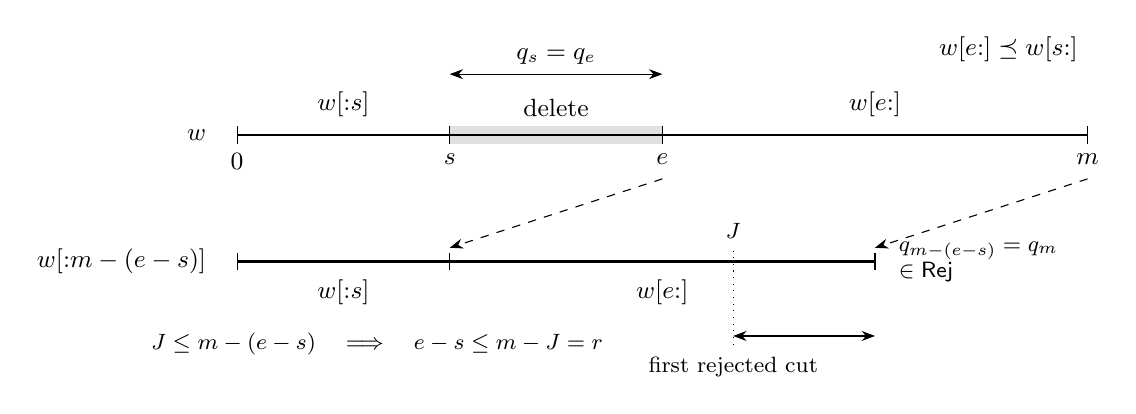
\begin{tikzpicture}[x=9mm,y=7mm,>=Stealth,font=\small]
  \node[anchor=east] at (-0.3,0) {$w$};
  \fill[black!12] (3,-0.16) rectangle (6,0.16);
  \draw[thick] (0,0) -- (12,0);
  \foreach \x/\lab in {0/0,3/s,6/e,12/m} {
    \draw (\x,-0.16) -- (\x,0.16);
    \node[below] at (\x,-0.16) {$\lab$};
  }
  \node[above] at (1.5,0.15) {$\wpre{w}{s}$};
  \node[above] at (4.5,0.15) {delete};
  \node[above] at (9,0.15) {$\wsuf{w}{e}$};
  \draw[<->] (3,1.1) -- (6,1.1)
    node[midway,above] {$q_s=q_e$};
  \node[anchor=east] at (12,1.55) {$\wsuf{w}{e}\pre\wsuf{w}{s}$};
  \draw[->,dashed] (6,-0.8) -- (3,-2.05);
  \draw[->,dashed] (12,-0.8) -- (9,-2.05);
  \node[anchor=east] at (-0.3,-2.3) {$\wpre{w}{m-(e-s)}$};
  \draw[thick] (0,-2.3) -- (9,-2.3);
  \foreach \x in {0,3,9} {\draw (\x,-2.46) -- (\x,-2.14);}
  \node[below] at (1.5,-2.45) {$\wpre{w}{s}$};
  \node[below] at (6,-2.45) {$\wsuf{w}{e}$};
  \node[anchor=west,align=left,font=\footnotesize] at (9.2,-2.3)
    {$q_{m-(e-s)}=q_m$\\$\in\Rej$};
  \draw[dotted] (7,-2.1) -- (7,-3.9);
  \node[above,font=\footnotesize] at (7,-2.05) {$J$};
  \draw[<->] (7,-3.65) -- (9,-3.65);
  \node[below,font=\footnotesize] at (7,-3.85) {first rejected cut};
  \node[anchor=east,font=\footnotesize] at (5.3,-3.8)
    {$J\le m-(e-s)\quad\Longrightarrow\quad e-s\le m-J=r$};
\end{tikzpicture}
\caption{The return gap (\cref{lem:return-gap}). A comparison makes loop deletion
produce the prefix $\wpre{w}{s}\wsuf{w}{e}=\wpre{w}{m-(e-s)}$.
Equal states at $s$ and $e$ preserve the final rejected state, so the shortened
prefix cannot end before $J$. The position of $J$ relative to $s,e$ is schematic;
only $J\le m-(e-s)$ is asserted.}
\Description{A word with cuts s, e, and m, and equal reader states at s and e.
Deleting the shaded interval from s to e moves the suffix to s, yielding a
shorter prefix in the same final rejected state. Its end is at or after the
first rejected cut J, bounding the deleted length by the rejected tail.}
\label{fig:return-gap}
\end{figure}


\subsection{The Depth Bound}

\begin{lemma}[Equal-support width]\label{lem:width}
Let $w$ be a nonempty rejected word with tail $r$, and let $j \le j'$ be levels with
$\Supp_j = \Supp_{j'} \ne \emptyset$. Then $j' - j + 1 \le r+1$.
\end{lemma}

\begin{proof}
For $j=j'$, the bound is immediate. Assume $j < j'$. Since $\Supp_{j'} \neq \emptyset$, all of $\Cores_j, \dots, \Cores_{j'}$ are nonempty.
By \cref{lem:cores}, $t_{i+1} < t_i$ for $j \le i < j'$, so $j' - j \le t_j - t_{j'}$. The state
$q_{t_j}$ lies in $\Supp_j = \Supp_{j'}$, so $q_s = q_{t_j}$ for some $s \in \Cores_{j'}$.
As $\Cores_{j'} \subseteq \Cores_{j+1}$, \cref{lem:cores} shows that $(s,t_j)$ is a comparison,
and \cref{lem:return-gap} gives $t_j - s \le r$. Since $s \le t_{j'}$, we obtain
$j' - j \le t_j - t_{j'} \le t_j - s \le r$.
\end{proof}

\begin{theorem}[Depth from tail]\label{thm:depth}
For every $N$-state reader, each nonempty rejected word with tail $r$ has
$\depth(w) \le 2N(r+1)-1$.
\end{theorem}

\begin{proof}
Let $d_w = \depth(w)$ and $R = r+1$. The supports $\Supp_0 \supseteq \Supp_1 \supseteq
\cdots \supseteq \Supp_{d_w}$ are nested, so the distinct nonempty ones form a strictly
decreasing chain of nonempty subsets of an $N$-element set, and there are at most $N$
of them. By \cref{lem:width}, each of them is the support of at most $R$ levels. Hence at
most $N R$ levels have nonempty support. If every level up to $d_w$ does, then
$d_w + 1 \le N R$. Otherwise, let $j_0$ be the first level with $\Supp_{j_0} = \emptyset$;
then $1 \le j_0 \le N R$, since $\Cores_0$ contains the cuts $0,\dots,\len{w}-1$. All cores
of $u_{j_0}$ are start cores, so $\len{u_{j_0}} \le j_0$ by \cref{lem:cores}. Each further
level up to $d_w$ strictly decreases the length, so $d_w - j_0 \le \len{u_{j_0}} - 1 \le j_0 - 1$,
and $d_w \le 2j_0 - 1 \le 2N R - 1$.
\end{proof}



\Cref{thm:depth} holds for every nonempty rejected word, hole or not; combined with
\cref{thm:brt}, it bounds the depth of some hole by $2N(4N-1)-1$.

\section{Bounded Depth Implies Bounded Length}
\label{sec:search}

The last bound turns a bound on the depth into a bound on the length. Like the depth bound,
it holds for every reader: it uses neither the admission cone nor any property of
non-structural subtype entailment.

\begin{theorem}[Bounded-depth search]\label{thm:search}
Let $(\mathcal{M},\Adm,\Rej)$ be any reader with $N$ states over a finite alphabet. If it has a
nonempty hole of depth at most $d$, then it has a nonempty hole of length at most
$\holeBound(N,d)$, where $\holeBound$ is the elementary function given in
\eqref{eq:holebound} below. The replacement can be chosen of depth at most $d$.
The same statement holds for any lettered monitor with $N$ states
(defined in \cref{sec:lettered}), even over an infinite alphabet.
\end{theorem}

The proof first bounds the number of distinct letters at every positive
level, then shortens a hole level by level along its hierarchy. Shortening each block of a
level independently fails, because comparisons relate \emph{different} blocks through equal
suffixes. We therefore shorten all blocks of a level \emph{simultaneously}, preserving a
finite summary of the whole tuple. As \cref{ex:loop-deletion} shows,
preserving the final reader state alone does not preserve holes.

\subsection{Lettered Monitors and Their Derivatives}\label{sec:lettered}

To describe each level of the hierarchy as a hole problem in its own right, we generalize
readers to \emph{lettered monitors}. A lettered monitor $\mathcal{M}$ over an alphabet
$\Gamma$, which may be infinite, consists of a finite set $\mathcal Q$ of states with a start state $\zeta_0$, a transition
function $\delta : \mathcal Q \times \Gamma \to \mathcal Q$, a \emph{final target} predicate
$\Tfin \subseteq \mathcal Q \times \Gamma$, and two admission relations $\Lambda$ and $\Lfin$ on
\emph{labels}, the second for comparisons that end at the final cut. Reading a word $v$
assigns the state $\zeta_{i+1} = \delta(\zeta_i, v[i])$ to cut $i+1$. The label of cut $0$ is a
symbol $\triangleright$, and the label of cut $i > 0$ is the pair $(\zeta_{i-1}, v[i-1])$ of the
state at cut $i-1$ and the letter read from it. A nonempty word $v$ is a \emph{hole} of
$\mathcal{M}$ if its last label $(\zeta,a)$ satisfies $\Tfin(\zeta,a)$, no terminal comparison
$(s,\len{v})$ satisfies $\Lfin$, and no other comparison $(s,e)$ satisfies $\Lambda$, each
relation being applied to the labels of the two cuts. A reader $(\mathcal{M},\Adm,\Rej)$ determines the
lettered monitor with states $Q$, the same transition $\delta$, $\Tfin(\zeta,a)$ iff $\delta(\zeta,a) \in \Rej$,
and $\Lambda = \Lfin$ given by $\Adm$ on the states that the labels denote: $\triangleright$
denotes $q_0$ and $(\zeta,a)$ denotes $\delta(\zeta,a)$. The reader and this lettered monitor have the same nonempty holes.
As with rejection, the final target only marks a candidate: a word whose last label
satisfies $\Tfin$ is a hole only if no comparison is admitted.
The predicate $\Tfin$ and the relations take labels, and not only the states
they denote, because the monitors of higher levels must evaluate them at positions
\emph{inside} blocks, which requires the letters. Block alphabets $(\Gamma\setminus\{\ell\})^*$
are generally infinite, even for finite $\Gamma$, so lettered monitors allow infinite
alphabets. The compression argument never uses finiteness of an alphabet: it works with
the finitely many letters that one hole uses and with finitely many summary values.

Fix a marker $\ell \in \Gamma$, a block $X \in (\Gamma \setminus \{\ell\})^*$, and a state
$\zeta \in \mathcal Q \sqcup \{\star\}$. The \emph{shifted block} of $X$ read from $\zeta \in \mathcal Q$ is the word
$\ell X$ read from $\zeta$; from the new symbol $\star$, it is $X$ read from $\zeta_0$. It has a label
$\mathit{lab}_p(\zeta,X)$ at each position $p = 0, \dots, \len{X}$: for $\zeta \in \mathcal Q$, the label of the
cut after $\ell\,\wpre{X}{p}$, so that position $0$ carries the \emph{marker label}
$(\zeta,\ell)$; for $\zeta = \star$, the label $\triangleright$ at position $0$ and the label of the cut
after $\wpre{X}{p}$ at positions $p \ge 1$. The \emph{exit state} $\delta_\ell(\zeta,X)$ is the
state reached at the end of the shifted block.

The derivative $\mathcal M_\ell$ defined next reads the block word. Each of its
letters represents an entire block, so the label of a derivative cut keeps both
the block and its entry state, the state from which the shifted block is read;
this lets the derivative recover every original label inside the block. With
these labels, $\mathcal M_\ell$ checks three kinds of obligations of the expanded
word. Its admission $\Lambda_\ell$ compares two positions in different blocks
that lie at the same distance from the ends of their blocks, with equal letters
after them. The second clause of its terminal admission $\Lfin_\ell$ compares a
position anywhere in an earlier block with the final cut, which carries the label
of the closing marker. Its target $\Tfin_\ell$ checks the original target together
with all terminal comparisons that start in the last block.

\begin{definition}[Derivative]\label{def:derivative}
Let $\mathcal{M}$ be a lettered monitor over $\Gamma$ with states $\mathcal Q$, and $\ell \in \Gamma$.
The \emph{derivative} $\mathcal{M}_\ell$ is the lettered monitor over the block alphabet
$(\Gamma\setminus\{\ell\})^*$ with states $\mathcal Q \sqcup \{\star\}$, start state $\star$, transition
function $\delta_\ell$, and the following relations on labels $(\zeta,X)$ and $(\zeta',X')$:
\begin{itemize}[leftmargin=*]
\item $\Lambda_\ell((\zeta,X),(\zeta',X'))$ holds if
  $\Lambda\bigl(\mathit{lab}_{p}(\zeta,X),\, \mathit{lab}_{p'}(\zeta',X')\bigr)$ for some
  positions $p\le\len{X}$ and $p'\le\len{X'}$ from which the two blocks have a common
  suffix, $\wsuf{X}{p}=\wsuf{X'}{p'}$;
\item $\Lfin_\ell((\zeta,X),(\zeta',X'))$ holds if $\Lambda_\ell((\zeta,X),(\zeta',X'))$ holds, or if
  $\Lfin\bigl(\mathit{lab}_p(\zeta,X), (\delta_\ell(\zeta',X'),\ell)\bigr)$ for some
  $p \le \len{X}$;
\item $\Tfin_\ell(\zeta,X)$ holds if $\Tfin(\delta_\ell(\zeta,X),\ell)$ holds and
  $\Lfin\bigl(\mathit{lab}_p(\zeta,X), (\delta_\ell(\zeta,X),\ell)\bigr)$ fails for every
  $p \le \len{X}$.
\end{itemize}
Every relation involving the label $\triangleright$ of $\mathcal{M}_\ell$ is false.
\end{definition}

The derivative's cut zero is an artificial boundary. Original comparisons
beginning at cut zero are represented inside the first shifted block,
whose entry state is $\star$; they are still tested through the label
$(\star,X_0)$. Setting relations at the derivative's new start label to
false therefore discards no original comparison.

For a concrete instance, use the reader of \cref{ex:loop-deletion}
on $0101$ and marker $1$. Its block word is $[0][0]$. The derivative
starts at $\star$ and reads $[0]$ to state $a$; from $a$, the shifted
block $10$ ends at $c$. The table shows which derivative label represents
each original cut.
\begin{center}
\small
\begin{tabular}{@{}lccccc@{}}
\toprule
original cut & $0$ & $1$ & $2$ & $3$ & $4$\\
state & $q$ & $a$ & $b$ & $c$ & $r$\\
original label & $\triangleright$ & $(q,0)$ & $(a,1)$ & $(b,0)$ & $(c,1)$\\
\midrule
derivative label & \multicolumn{2}{c}{$(\star,[0])$} & \multicolumn{2}{c}{$(a,[0])$} & final\\
\cmidrule(lr){2-3}\cmidrule(lr){4-5}
position $p$ in its block & $0$ & $1$ & $0$ & $1$ & \\
\bottomrule
\end{tabular}
\end{center}
The two derivative labels sit at the derivative cuts $1$ and $2$, and each
represents the original cuts of one shifted block: the first block is read from
the start, and the second begins with the marker label $(a,1)$. The final original
cut carries the label $(c,1)$ of the closing marker, read from the final derivative
state $c$. For the two derivative labels, the common suffix $0$ selects position
zero in both blocks. Their original labels denote $q$ and $\delta(a,1)=b$, so
$\Lambda_1$ holds. The derivative comparison $(1,2)$ is terminal and its $\Lfin_1$
relation therefore holds as well. It detects the original nonterminal comparison
$(0,2)$, including its start at the original cut zero.

\begin{lemma}[Holes under desubstitution]\label{lem:der-holes}
Let $v$ be a nonempty word of blocks that avoid $\ell$, and let $u$ be its expansion. Then
$u$ is a hole of $\mathcal{M}$ iff $v$ is a hole of $\mathcal{M}_\ell$. Consequently, if
$\mathcal{M}_0$ is a reader with $N$ states and $\mathcal{M}_{j+1} = (\mathcal{M}_j)_{\ell_j}$
along the canonical hierarchy of $w$, then $w$ is a hole of $\mathcal{M}_0$ iff $u_j$ is a
hole of $\mathcal{M}_j$, and $\mathcal{M}_j$ has $N + j$ states.
\end{lemma}

\begin{proof}
Write $v=[X_0]\cdots[X_{h-1}]$, so
$u=X_0\ell X_1\ell\cdots X_{h-1}\ell$, and let
$\zeta'_0=\star,\zeta'_1,\ldots,\zeta'_h$ be the derivative run.
Let $a_i$ be the cut where $X_i$ begins and $b_i=a_i+|X_i|$ the
position of its closing marker. Partition all nonfinal cuts of $u$ into
the intervals $[a_i,b_i]$. Induction on $i$ gives the label
$\mathit{lab}_p(\zeta'_i,X_i)$ at cut $a_i+p$, for $0\le p\le|X_i|$;
the final cut has label $(\zeta'_h,\ell)$. The label of cut $i+1$ of $v$
is $(\zeta'_i,X_i)$, so it determines every label in this block.

Suppose first that $u$ is a hole. Its final target holds, and none of
its terminal comparisons starting in the last block is admitted. These
are exactly the two requirements of $\Tfin_\ell(\zeta'_{h-1},X_{h-1})$.
Consider a comparison $(s',e')$ of $v$. If $s'=0$, its relations are false
by definition. Otherwise, $1\le s'<e'\le h$. If $\Lambda_\ell$ held at its
labels, it would supply positions $p$ in $X_{s'-1}$ and $p'$ in $X_{e'-1}$
with $\wsuf{X_{s'-1}}{p}=\wsuf{X_{e'-1}}{p'}$.
The cuts $s=a_{s'-1}+p$ and $e=a_{e'-1}+p'$ have this common
suffix before their markers. By \cref{lem:alignment}, $(s,e)$ is
a comparison of $u$; it is nonterminal even when $e'=h$, since
$e\le b_{h-1}<|u|$. Its labels would satisfy $\Lambda$, a contradiction.
This excludes $\Lambda_\ell$ both at nonterminal comparisons of $v$
and as the first disjunct of $\Lfin_\ell$ at terminal ones.
The second disjunct, possible only for $e'=h$, gives an admitted terminal
comparison $(a_{s'-1}+p,|u|)$ of $u$ for some position $p$, also a
contradiction. Thus $v$ is a hole.

Conversely, suppose $v$ is a hole. Its target implies the final target
of $u$ and excludes every admitted terminal comparison starting in the
last block. Let $(s,e)$ be any other comparison of $u$. If $e<|u|$,
\cref{lem:alignment} locates $s,e$ in blocks $s'-1,e'-1$ with $s'<e'$,
a common suffix after them, and a comparison $(s',e')$ of $v$.
Admission by $\Lambda$ would therefore give $\Lambda_\ell$ at its labels.
For $e'<h$ this contradicts the nonterminal hole condition of $v$;
for $e'=h$ it contradicts the first disjunct of its terminal relation
$\Lfin_\ell$. If $e=|u|$, its start is in an earlier block $s'-1$
with $s'<h$. Then $(s',h)$ is a terminal comparison of $v$, and admission
by $\Lfin$ would give the second disjunct of $\Lfin_\ell$.
Again this is impossible. All comparisons of $u$ are therefore unadmitted,
so $u$ is a hole. Iterating this equivalence proves the hierarchy assertion;
each derivative adds exactly one fresh state.
\end{proof}



\subsection{Isolated Exchange and Bounded Dictionaries}
\label{sec:dictionary}

Shortening (\cref{sec:shortening}) compresses all distinct blocks of a level at
once, and its length bound grows quickly with the number of these blocks. We
therefore need a bound on the number of different blocks at each positive level,
not just on their lengths. We obtain it by merging letters that have the same
effect on the derived monitor. Such a merge must preserve the comparisons of the
level word as well as its transitions, targets, and admissions. We therefore
protect the marker and the letters at symbolic start positions, and merge only
letters whose unequal comparison partners are all protected. The behavior of such
a letter can then be recorded in finite tables, its exchange type, whose size does
not depend on the dictionary. The other letters are counted through the boundary
pairs defined below, and these counts propagate from one level to the next.

Fix a nonempty hole $w$ of depth $\Delta\le d$, its hierarchy $u_i$, and
its derived monitors $\mathcal M_i$. For a word $v$, let
$\operatorname{alph}(v)$ be its set of letters. Write
$\mathcal A_i=\operatorname{alph}(u_i)$ for the level-$i$
\emph{dictionary}, and
$g_i=|\mathcal A_i|$. These are letter dictionaries, distinct from the
state supports $\Supp_i$ of \cref{sec:depth}. A comparison at level $i$
is a comparison of $u_i$ in the sense of \cref{def:comparison}.
It is \emph{left maximal} if $1\le s<e\le |u_i|$ and its predecessor
letters $u_i[s-1]$ and $u_i[e-1]$ differ, so that it cannot be extended one
letter to the left. Comparisons that begin at cut zero are excluded: they
have no predecessor letter, and their admissions involve the start label,
which the exchange types below record separately. The \emph{boundary pairs}
of level $i$ are the ordered letter pairs
\[
 \operatorname{BP}_i=\{(u_i[s-1],u_i[e-1]):
       (s,e)\text{ is left maximal},\ e<|u_i|\},
\]
counted once regardless of how many comparisons produce them; put
$b_i=|\operatorname{BP}_i|$. A left-maximal comparison that ends at the
final cut has the marker $\ell_i$ as its second predecessor letter, since
$u_i$ ends with $\ell_i$. Its pair, an endpoint pair, is needed only in the
proofs (\cref{app:search}).

The positions of $u_i$ with start cores form a prefix, and their number
$s_i\le i$ is the \emph{start count} of level $i$ (\cref{lem:cores}). In the
derived monitor, ordinary positions are read from the embedded copy of the
original state set $Q$, and start positions from symbolic states. Let $Z_i$
be the union of that copy of $Q$ and the symbolic states used at start
positions; then $|Z_i|\le N+s_i$. The \emph{protected letters} of level $i$ are
\[
 \Pi_i=\{\ell_i\}\cup\operatorname{alph}(u_i[:s_i]),
 \qquad |\Pi_i|\le s_i+1.
\]
A letter $a\in\mathcal A_i\setminus\Pi_i$ is \emph{isolated} if no
boundary pair has $a$ as one component and a letter outside $\Pi_i$ as the
other. All unequal comparison partners of an isolated letter are therefore
protected, including its partner in terminal comparisons, the marker.

\begin{example}[Protected and isolated letters]\label{ex:isolated}
At level $1$ of \cref{ex:hierarchy}, the word $u_1=\alpha_1\beta_1\gamma_1\alpha_1$
has cores $\star_1,1,4,5$ and marker $\ell_1=\alpha_1$. Its start count is
$s_1=1$ and its start prefix is $\alpha_1$, so $\Pi_1=\{\alpha_1\}$. The only
comparison of $u_1$ that ends before the final cut is $(0,3)$, which begins at
cut zero. Hence $\operatorname{BP}_1=\varnothing$, and $\beta_1$ and $\gamma_1$
are isolated. Their only unequal comparison partner is the marker, through the
terminal comparisons $(2,4)$ and $(3,4)$. Merging $\beta_1$ and $\gamma_1$ would
therefore preserve the comparisons of $u_1$; it would also require equal exchange
types, defined next, which depend on the monitor.
\end{example}

For an isolated letter $a$, its \emph{exchange type relative to $\Pi_i$}
records the following finite tables in $\mathcal M_i$:
\begin{itemize}[leftmargin=*]
\item the transition $q\mapsto\delta_i(q,a)$ and target
  $\Tfin_i(q,a)$ for every ordinary state $q\in Q$;
\item for each $R\in\{\Lambda_i,\Lfin_i\}$, the self table
  $R((q,a),(q',a))$ for $q,q'\in Q$;
\item for each such $R$, both $R((q,a),(\zeta,\pi))$ and
  $R((\zeta,\pi),(q,a))$ for $q\in Q$, $\zeta\in Z_i$, $\pi\in\Pi_i$;
\item the two initial-label rows $R(\triangleright,(q,a))$ for $q\in Q$.
\end{itemize}
At positive levels the last rows are false. Original cut-zero obligations
are still recorded in the protected rows at symbolic entry states
(rows $R((q,a),(\zeta,\pi))$ and their reverse orientations, with $\zeta$ symbolic
and $\pi$ in the start prefix).
Ordinary states transition to ordinary states, so the transition table has
$N^N$ possibilities, rather than $(N+i)^N$.

Put
\begin{equation}\label{eq:dictionary-constants}
\begin{aligned}
 \TyBound(N,d)&=N^N\,2^{2N^2+4N(N+d)(d+1)+3N},\\
 \AlBound(N,d)&=d+1+\TyBound(N,d),&
 \DictBound(N,d)&=2+\AlBound(N,d)3^d.
\end{aligned}
\end{equation}
Here $\TyBound$ bounds the number of exchange types, $\AlBound$ adds the
protected letters, and $\DictBound$ will bound every positive dictionary.
Shortening a tuple of $h$ blocks produces blocks shorter than
$\mathit{col}(M,h)$, the column count of \eqref{eq:col} for a monitor with $M$
states, which for fixed $M$ is exponential in $h^2$. Bounding every positive
dictionary by $\DictBound(N,d)$ in advance makes each of at most $d$ expansion
steps multiply lengths by at most the fixed factor
$K=\mathit{col}(N+d+1,\DictBound(N,d))$. The exchange argument achieves such a bound
by merging only isolated letters: their types need rows only against the
at most $d+1$ protected letters, so $\TyBound(N,d)$ is independent of dictionary
sizes. Extending this rule to non-isolated letters would require protecting
their unequal comparison partners as well; their number would enter the
type-count exponent and could compound from level to level.

\begin{lemma}[Exchange types]\label{lem:exchange-types}
At every positive level $i<\Delta\le d$, there are at most $\TyBound(N,d)$
exchange types relative to $\Pi_i$.
\end{lemma}

\begin{lemma}[Isolated exchange]\label{lem:isolated-exchange}
Let $1\le i<\Delta$, and let distinct isolated letters $a,a'$ of $u_i$
have the same exchange type. Replace every $a$ by $a'$ at that level
and expand using the markers of the original hierarchy below level $i$. The
result is a hole of the same canonical depth, with every start count unchanged
and no dictionary larger. Its level-$i$ dictionary is strictly smaller. Choosing
the direction toward the letter with shorter level-zero expansion also makes the
word no longer.
\end{lemma}

Call a hole \emph{dictionary-normal} if, at every $1\le i<\Delta$, distinct isolated
letters have distinct exchange types, computed in that hole's own hierarchy.
\begin{lemma}[Dictionary normal form]\label{lem:dictionary-normal-form}
Every nonempty hole has a dictionary-normal hole of the same depth, no greater
length, the same start counts, and no larger dictionary at any level.
\end{lemma}
\begin{lemma}[Dictionary counting and propagation]\label{lem:dictionary-count}
For a dictionary-normal hole of depth $\Delta\le d$, and $1\le i<\Delta$,
$g_i\le \AlBound(N,d)+2b_i$.
For every nonempty word and every level $i$,
\begin{equation}\label{eq:boundary-propagation}
 b_i\le b_{i+1}+g_{i+1}-1.
\end{equation}
\end{lemma}
\begin{lemma}[Bounded dictionaries]\label{lem:dictionary-bound}
For a dictionary-normal hole of depth $\Delta\le d$, at $1\le i<\Delta$,
\begin{equation}\label{eq:dictionary-recurrence}
 2b_i\le(\AlBound(N,d)-1)(3^{\Delta-1-i}-1),\qquad
 g_i\le1+(\AlBound(N,d)-1)3^{\Delta-1-i}.
\end{equation}
Consequently every nonempty hole of depth at most $d$ has a hole of the
same depth and no greater length with $g_i\le \DictBound(N,d)$ for every
$1\le i\le \Delta$. No bound on $g_0$ is required.
\end{lemma}

Full proofs, including preservation of start counts under the induced
level maps, appear in \cref{app:search}. The counting idea is simple:
dictionary normality bounds isolated letters by their types, while each remaining
unprotected letter is a component of a boundary pair. This adds at most
$2b_i$ letters. Those letters need not enter the protected set
inside the type-count exponent: an isolated letter never compares with
an unprotected unequal partner. Propagation therefore gives a linear
recurrence with factor three, while the type bound remains fixed.

\subsection{Shortening}\label{sec:shortening}

Fix the dictionary-normal hole and its dictionaries $\mathcal A_j$. Throughout
shortening, the original hierarchy means the hierarchy of this hole, which stays
unchanged. Put $g=\DictBound(N,d)$ and
$K=\mathit{col}(N+d+1,g)$, using the column count of \eqref{eq:col}.
We shorten top-down.
First the top level is shortened; then the blocks that form its
letters; then the blocks that form the letters of those blocks; and so on down to level~$0$.

\paragraph{The Top Level}
At the first unary level $\Delta\le d$, write $u_\Delta = z^L$. Every pair of its cuts is a
comparison, and its states follow the orbit of $\delta(\cdot,z)$. Deleting the letters between
two nonfinal cuts with equal states creates no new kind of label pair, so a unary hole of
$\mathcal{M}_\Delta$ can be shortened to at most $N + \Delta$ letters, the number of states
(details in \cref{app:search}).

\begin{figure}[tbp]
\centering
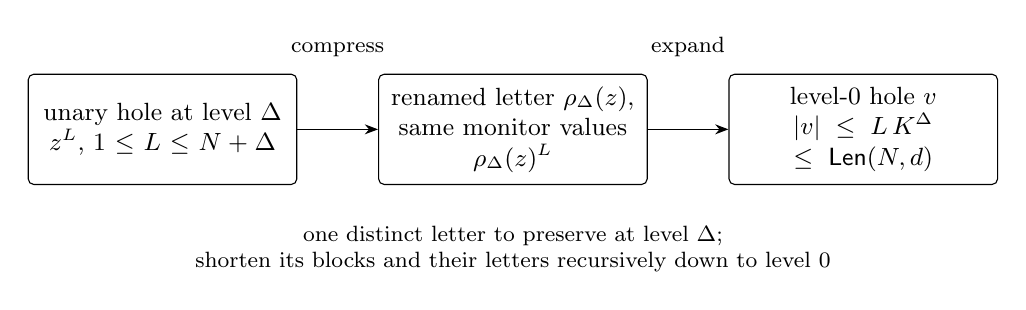
\begin{tikzpicture}[>=Stealth,font=\small,
  stage/.style={draw,rounded corners=2pt,align=center,text width=32mm,
    minimum height=14mm,inner sep=3pt}]
  \node[stage] (unary) at (0,0)
    {unary hole at level $\Delta$\\$z^L$, $1\le L\le N+\Delta$};
  \node[stage] (compressed) at (4.45,0)
    {renamed letter $\rho_\Delta(z)$,\\same monitor values\\$\rho_\Delta(z)^L$};
  \node[stage] (expanded) at (8.9,0)
    {level-$0$ hole $v$\\$|v|\le L\,K^\Delta$\\$\le\holeBound(N,d)$};
  \draw[->] (unary) -- (compressed)
    node[midway,above=8mm,font=\footnotesize] {compress};
  \draw[->] (compressed) -- (expanded)
    node[midway,above=8mm,font=\footnotesize] {expand};
  \node[below=4mm of compressed,align=center,font=\footnotesize]
    {one distinct letter to preserve at level $\Delta$;\\
     shorten its blocks and their letters recursively down to level $0$};
\end{tikzpicture}
\caption{Unary top level and compression. First shorten the unary power by
deleting repeated-state loops, giving $L\le N+\Delta$. Compression then renames
its single letter by the injective renaming $\rho_\Delta$ of
\cref{lem:simultaneous-compression}, under which the new level-$\Delta$ monitor
agrees with the original one: it has the same transition, target, and admission
values on the renamed letter. This preserves the run, target, and admissions of the power.
With the dictionary-normal hierarchy unchanged and
$K=\mathit{col}(N+d+1,\DictBound(N,d))$, supported block compression bounds
that letter's expansion by $K^\Delta$, giving
$|v|\le LK^\Delta\le\holeBound(N,d)$. At $\Delta=0$ the expansion is the identity.}
\Description{Three boxes show a unary hole with at most N plus Delta copies of one
letter, an injective renaming preserving monitor agreement, and expansion to a
level-zero hole of length at most L times the Delta-th power of the fixed column bound.}
\label{fig:unary-compression}
\end{figure}


\paragraph{The Block Levels}
At level $j+1$, select distinct original blocks $X_1,\dots,X_h$ from
$\mathcal A_{j+1}$. They are words over $\mathcal A_j$ avoiding the
original marker $\ell_j$. The \emph{summary} of the tuple
$(X_1,\dots,X_h)$ with respect to $\mathcal{M}_j$ and $\ell_j$ records:
\begin{itemize}[leftmargin=*]
\item for each block and each state $\zeta \in \mathcal Q \sqcup \{\star\}$, the exit state of its shifted
  block read from~$\zeta$;
\item for each block, each such $\zeta$, and each state $\zeta''\in\mathcal Q$, whether some label of the shifted
  block read from $\zeta$ is related by $\Lfin$ to the final label $(\zeta'',\ell_j)$;
\item which blocks are equal;
\item for each ordered pair of blocks and each pair of states $\zeta, \zeta'$, whether
  $\Lambda_{\ell_j}$ relates the two labels.
\end{itemize}
The summary determines every value of $\mathcal{M}_{j+1}$ on the letters $X_1,\dots,X_h$,
together with their equalities. Storing all equality bits preserves
disequality as well: distinct old letters get distinct replacements, so
the replacement is injective. It can be computed by a deterministic finite automaton
reading the tuple as a single word of \emph{columns}: align the blocks at their right ends,
pad them on the left, and read the $h$-tuples of optional letters from left to right
(\cref{fig:columns}). Right alignment is what makes this possible: $\Lambda_{\ell_j}$
compares positions at equal distance from the ends of two blocks with equal letters after
them, so appending a column either relates the two new last positions, or extends the
common suffix of a pair related earlier by an equal letter. A column word is
\emph{valid} if each of its tracks consists of absent entries followed by letters, as
padding on the left requires. If the column word has at least as many columns as there
are summary values, two cuts have the same summary. Deleting the columns between them
preserves the summary. It also preserves validity without any extra state in the
automaton: deleting columns keeps every track of the form ``absent entries, then
letters'', and each column itself records which tracks are present. Repeating this, we
obtain blocks $\widetilde X_1,\dots,\widetilde X_h$ of length less than the number
$\mathit{col}(N+j,h)$ of summary values, with the same summary. Substituting
$\widetilde X_i$ for $X_i$ yields a word that is again a hole of $\mathcal{M}_{j+1}$.

\begin{figure}[tbp]
\centering
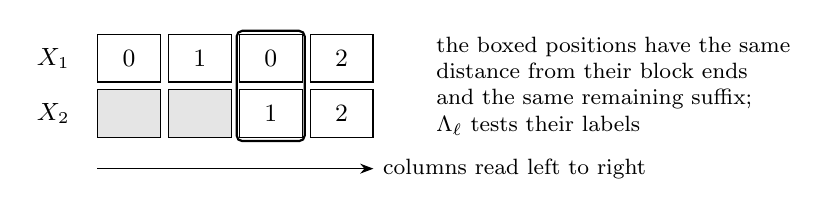
\begin{tikzpicture}[x=9mm,y=7mm,>=Stealth,
    cell/.style={draw, minimum width=8mm, minimum height=6mm, inner sep=1pt, font=\small}]
  \node[anchor=east,font=\small] at (-0.7,0) {$X_1$};
  \node[anchor=east,font=\small] at (-0.7,-1) {$X_2$};
  \node[cell] at (0,0) {$0$};
  \node[cell] at (1,0) {$1$};
  \node[cell] at (2,0) {$0$};
  \node[cell] at (3,0) {$2$};
  \node[cell,fill=black!10] at (0,-1) {};
  \node[cell,fill=black!10] at (1,-1) {};
  \node[cell] at (2,-1) {$1$};
  \node[cell] at (3,-1) {$2$};
  \draw[thick,rounded corners=2pt] (1.52,0.5) rectangle (2.48,-1.5);
  \draw[->] (-0.45,-2.0) -- (3.45,-2.0) node[right,font=\footnotesize] {columns read left to right};
  \node[font=\footnotesize,align=left,anchor=west] at (4.2,-0.5)
    {the boxed positions have the same\\distance from their block ends\\and the same remaining suffix;\\$\Lambda_\ell$ tests their labels};
\end{tikzpicture}
\caption{The column encoding of a tuple of blocks, here $X_1 = 0102$ and $X_2 = 12$. The
blocks are aligned at their right ends and padded on the left (shaded cells). A deterministic
automaton reads the columns from left to right and maintains the summary of the tuple: the
exit states of the shifted blocks, their tests against the final label, the equalities between blocks, and the
bits of $\Lambda_\ell$. Deleting the columns between two equal summaries shortens all blocks
at once and preserves the summary (\cref{app:search}).}
\Description{Two blocks aligned at their right ends, the shorter one padded on the left, with one column highlighted.}
\label{fig:columns}
\end{figure}

The recursion keeps a set $\mathcal E_{j+1}\subseteq\mathcal A_{j+1}$ of distinct
original letters, its \emph{letter support}. After shortening its blocks to
subsequences $\tau(X)$, form the lower letter support
\begin{equation}\label{eq:descent-support}
 \mathcal E_j=\{\ell_j\}\cup\bigcup_{X\in\mathcal E_{j+1}}\operatorname{alph}(\tau(X))
 \ \subseteq\ \mathcal A_j.
\end{equation}
The inclusion holds because every letter of an original upper block
belongs to the original lower dictionary, and shortening only deletes
letters. Thus each column shortening involves at most $g$ blocks (tracks).
At level zero no column shortening is needed, so its support need not have
size at most $g$.

Compression proceeds top-down and renames letters as it goes. Shortening the
level-$(j+1)$ blocks changes which level-$j$ letters occur; those letters are
shortened in turn, so the level-$j$ marker and every lower derived monitor change
as well. We therefore never compare the compressed word with the original
hierarchy directly. Instead we keep, at each level $j$, an injective renaming
$\rho_j$ of the letter support $\mathcal E_j$ under which the new derived monitor
\emph{agrees} with the original one: it has the same transitions, targets, and both
admission relations on the renamed letters, at every state, including the symbolic
states and the start label \eqref{eq:monitor-agreement}. Agreement up to an injective
renaming suffices because a monitor sees letters only through these values and
through equality of letters, and an injective renaming preserves both equality and
inequality. Hence agreement preserves comparisons, runs, and holes. Since the support
contains the marker, injectivity also preserves marker avoidance.
\Cref{lem:simultaneous-compression} composes the agreement given by the column
summaries with agreement at the level below. Each level multiplies expansion lengths
by at most $K$, so a renamed level-$j$ letter expands to at most $K^j$ letters. The
original hierarchy and dictionaries stay unchanged throughout this induction;
intermediate compressed words need not be dictionary-normal.

\paragraph{The Bound}
For a lettered monitor with $N$ states and a tuple of $h$ blocks, put
\begin{equation}\label{eq:col}
  \mathit{col}(N,h) = N^{(N+1)h}\cdot 2^{N(N+1)h}\cdot 2^{h^2}\cdot 2^{(N+1)^2h^2}.
\end{equation}
This product counts all assignments to the summary fields and therefore
bounds the number of reachable summary states.
\begin{center}
\begin{tabular}{@{}ll@{}}
\toprule
Factor & Summary field\\
\midrule
$N^{(N+1)h}$ & Exit states: $h$ blocks, $N+1$ entry states\\
$2^{N(N+1)h}$ & Terminal-comparison bits: also $N$ final-marker states\\
$2^{h^2}$ & Equality bits for ordered pairs of blocks\\
$2^{(N+1)^2h^2}$ & Derived-admission bits for block and entry-state pairs\\
\bottomrule
\end{tabular}
\end{center}
Each shortened block has fewer than $\mathit{col}(N+j,g)\le K$
letters, so with its closing marker it has at most $K$ letters. Expanding down
one level therefore multiplies lengths by at most $K$. The unary top has at most
$N+\Delta$ letters, and there are $\Delta\le d$ expansions. Define the single length bound
\begin{equation}\label{eq:holebound}
 \holeBound(N,d)=(N+d+1)\,
       \mathit{col}\bigl(N+d+1,\DictBound(N,d)\bigr)^d.
\end{equation}
The resulting nonempty hole has depth at most $d$ and length at most
$(N+\Delta)K^\Delta\le\holeBound(N,d)$, proving \cref{thm:search}.
The alphabet size does not enter the bound. \Cref{sec:complexity}
gives a closed-form estimate and distinguishes hole length from
exhaustive enumeration cost.

\FloatBarrier

\section{Deciding Entailment in the Three Domains}
\label{sec:decision}

This section assembles the three bounds into decision procedures: a finite
search for holes, a procedure for arbitrary trees built on it
(\cref{fig:algorithm}), and transfers to regular and finite trees.

\begin{theorem}[Finite search for holes]\label{thm:hole-decision}
For an $N$-state reader, over any finite alphabet, that satisfies the
rejected-path property, put
\begin{equation}\label{eq:bounds}
 B=4N-2,\qquad d=2N(B+1)-1,\qquad H=\holeBound(N,d).
\end{equation}
A hole exists iff a hole of length at most $H$ exists, where $\holeBound$
is given by \eqref{eq:holebound}. Moreover,
$H\le2^{2^{1280(N+1)^5}}$.
\end{theorem}
\begin{proof}
By \cref{thm:brt}, choose a hole with tail at most $B$. If it is empty,
it already meets the bound. Otherwise, \cref{thm:depth} bounds its depth by
$d$ in the original $N$-state reader. Applying \cref{thm:search} gives a
hole of length at most $H$. For an empty alphabet only
$\eps$ exists, so no nonempty hierarchy is required. The reverse implication
is immediate. The closed-form estimate is \cref{lem:elementary-estimate}.
Each candidate can be checked by computing its run and
examining the finitely many pairs $s<e\le |w|$.
\end{proof}

\begin{figure}[t]
\small
\begin{minipage}{0.94\linewidth}
\textbf{Input:} arity $n$, variance $c$, a flat system $\phi$ on $k$ variables,
and query $x\le y$.\\
\textbf{Output:} whether $\phi\models_c x\le y$.
\begin{enumerate}[leftmargin=*,itemsep=2pt]
\item Form $\psi=\phi^\pm$, compute its closure, and test for a label clash.
If a clash exists, return \emph{yes}.
\item Instantiate the reader of \cref{sec:label-reader} on $\psi$ with the
roots $(x^+,y^+)$ and with the roots $(y^-,x^-)$.
Use $N=2\cdot4^{2k}$ and compute $B,d,H$ from \eqref{eq:bounds}.
\item Enumerate all words in $\Dir^*$ of length at most $H$, including
$\eps$. If either reader has a hole, return \emph{no}; otherwise return
\emph{yes}. (\Cref{sec:complexity} replaces this enumeration by the
summary search of \cref{prop:summary-search}.)
\end{enumerate}
For regular trees, use the same answer. For finite trees, first test finite
satisfiability; if it fails, return \emph{yes}, otherwise use the same answer.
\end{minipage}
\caption{The decision procedure for flat constraints and a variable query.}
\Description{A satisfiability test followed by two bounded searches for label-reader holes, with domain transfers for regular and finite trees.}
\label{fig:algorithm}
\end{figure}

\begin{theorem}[Correctness]\label{thm:correct}
The procedure of \cref{fig:algorithm} decides arbitrary-tree entailment.
\end{theorem}
\begin{proof}
By \cref{lem:selector}, \eqref{eq:g19}, and \cref{thm:sat}, step~1 returns yes exactly
when no solution exists. Otherwise, \eqref{eq:g13} and \cref{thm:holes} give
\[
 \phi\models_c x\le y\quad\Longleftrightarrow\quad
 \text{neither label reader has a hole}.
\]
Both readers satisfy the rejected-path property. By
\cref{thm:hole-decision}, the bounded search finds a hole whenever one exists.
Thus each answer is correct, and the finite enumeration terminates.
\end{proof}

\subsection{Regular and Finite Transfers}
Finite trees need one test beyond the label clash. A \emph{cycle clash} of
a covariant system $\chi$ is a nonempty word $\eta$ together with
variables $a,b$ such that
\begin{equation}\label{eq:g55}
 \Lo(\eta,a,a),\qquad D_\chi(a,b),\qquad \Up(\eta,b,b).
\end{equation}
In every solution $\sigma$ they give
$\emb_\bot(\eta,\sigma(a))\le\sigma(a)\le\sigma(b)\le\emb_\top(\eta,\sigma(b))$
by \eqref{eq:g23}. Iterating the two self-bounds forces constructor paths
along every power of $\eta$, so a cycle clash excludes finite solutions.

\begin{proposition}[Transfer]\label{prop:transfer}
For every arity and variance,
\begin{align}
 \phi\models_{\mathrm{reg},c}x\le y
 &\quad\Longleftrightarrow\quad\phi\models_c x\le y,\label{eq:g7}\\
 \phi\models_{\mathrm{fin},c}x\le y
 &\quad\Longleftrightarrow\quad
 \neg\Sat_{\mathrm{fin},c}(\phi)\ \lor\ \phi\models_c x\le y,\label{eq:g8}\\
 \Sat_{\mathrm{reg},c}(\phi)
 &\quad\Longleftrightarrow\quad\Sat_c(\phi).\label{eq:sat-reg}
\end{align}
Finite satisfiability is decidable.
\end{proposition}

\begin{proof}
The least shape is the unfolding of a finite graph of pairs of upper
and lower supporting-variable sets. Selection and decoding are realized
by graph products with polarity bits. Applying these operations to the
same four-spine extension as in \cref{thm:four-spine} gives a regular
countermodel whenever an arbitrary countermodel exists; the reverse
implication is immediate. The same operations applied to $\psi$ itself, without
spines, give a regular solution whenever a solution exists, which proves
\eqref{eq:sat-reg}.
The full graph construction and its equality
with the pruned least shape are proved in \cref{thm:shape-graph,thm:regular-transfer}.

For finite satisfiability, a covariant system must have neither a label
clash nor a cycle clash \eqref{eq:g55}. These conditions are sufficient by
\cref{thm:finite-sat}. Without a cycle clash the least shape has depth at
most $k_\chi^2+1$ for $k_\chi$ covariant variables; a longer constructor
path repeats a pair of supporting variables and yields a cycle clash.
A finite graph on such pairs decides the cycle test. Selection preserves
the finite domain, and decoding gives the finite signed correspondence
of \cref{lem:finite-signed}.

Finally, suppose the base has a finite solution and an arbitrary
countermodel. Its unsafe word has a clash-free four-spine extension.
Sources and sinks are separated. Assign old variables rank zero, new
spine variables their cut indices, and fillers rank $|w|+1$; ranks increase
along new constructor edges, so every cycle clash would reflect to the
base. The finite solution is used only to exclude cycle clashes in the
base. The extension preserves that exclusion, and its least shape can
therefore be reconstructed independently with bounded depth. Its selected fixed solution restricts and decodes to a
finite countermodel with the same unsafe word. This gives the finite
entailment equivalence, including the stated vacuity case; all rank and
depth details are proved in \cref{thm:finite-transfer}.
\end{proof}

The finite vacuity case is necessary: at positive arity the constraint
$f(x,\ldots,x)\le x\le f(x,\ldots,x)$ forces the infinite constructor
tree. It has no finite solution. For $n=0$, the reader search examines only
$\eps$, and the terminal child test still checks for a constructor bound.
Together with \cref{thm:correct}, the transfer proves \cref{thm:main}.

The effective graph-size and finite-depth bounds are collected in
\cref{sec:countermodel-bounds}.

The enumeration of \cref{fig:algorithm} establishes decidability.
\Cref{sec:complexity} implements its hole search differently: the summary
search (\cref{prop:summary-search}) stores one level of the block hierarchy
instead of a word and yields the space bound (\cref{thm:complexity}).

\section{Complexity}
\label{sec:complexity}

This section bounds the cost of deciding entailment. The input lists the
arity $n$, the variance table $c(0),\ldots,c(n-1)$, the variable set $V$, the
query, and the literals of $\phi$, each constructor literal listing all $n$
child variables. Write $\insize\phi$ for its size; thus $n\le\insize\phi$ and
$k=|V|\le\insize\phi$. The readers of \cref{sec:label-reader} have
$N=2\cdot4^{2k}=2^{4k+1}$ states. The constants hidden in $O$-notation below
are absolute: they depend neither on $n$, nor on $c$, nor on the domain. We
write 2-EXPSPACE for the problems decidable in deterministic space
$2^{2^{p(\insize\phi)}}$, and 3-EXPTIME for those decidable in deterministic
time $2^{2^{2^{p(\insize\phi)}}}$, for polynomials $p$. Deterministic
classes, such as these and PSPACE, are closed under complement, so their
bounds hold for entailment and non-entailment alike.

This section concentrates on constructors of arity $n\ge2$.
\Cref{sec:complexity-upper} proves an upper bound that holds for every
arity: a search that stores one level of the block hierarchy at a time places
entailment in 2-EXPSPACE and in 3-EXPTIME. For $n\le1$ stronger bounds hold,
PSPACE at arity one and polynomial time at arity zero
(\cref{app:small-arity}). \Cref{sec:complexity-lower} proves lower bounds for
a covariant constructor of each fixed arity $n\ge2$: shortest holes can be
exponentially long in $k$, and entailment is PSPACE-hard. All these bounds
hold in each of the three domains.

\subsection{Upper Bounds}
\label{sec:complexity-upper}

\paragraph{Hole Length}
The constants of \eqref{eq:bounds} are $B=4N-2$, $d=8N^2-2N-1$, and
$H=\holeBound(N,d)$. By \cref{thm:hole-decision,lem:elementary-estimate},
\[
 H\le2^{2^{1280(N+1)^5}},
\]
a triply exponential bound $2^{2^{2^{O(k)}}}$ in $k$. When $\phi$ is
satisfiable in the domain considered and the entailment fails, a hole of
length at most $H$ of one of the two label readers certifies the failure
(\cref{thm:holes,prop:transfer}). It is an unsafe word, and it can be checked
in time polynomial in its length and in $\insize\phi$. The bound concerns the
length of an unsafe word, not the node count of a fully expanded
countermodel. Enumerating all words up to length $H$, as \cref{fig:algorithm}
does, examines $\sum_{L\le H}n^L$ words per reader, four exponentials in $k$
for fixed $n\ge2$. The summary search below decides the same question without
storing a word.

\paragraph{Polynomial-Time Tests}
Every test of the reduction other than the search for holes is cheap.

\begin{lemma}[Polynomial-time tests]\label{lem:poly-tests}
From a flat system $\phi$ with $k$ variables and the query, the following are
computable in time polynomial in $\insize\phi$: the signed system
$\psi=\phi^\pm$ and its closure; whether it has a
label clash or a cycle clash; and, for either label reader and states given
as bit vectors, the initial state, the successor of a state under a letter,
whether a state is rejected, and whether a pair of states is admitted. In
particular, $\Sat_{\mathcal D,c}(\phi)$ is decidable in polynomial time for
each of the three domains $\mathcal D$.
\end{lemma}

The closure has at most $(2k)^2$ pairs and is computed by saturation. Every
reader operation is a set operation on the $2k$ signed variables, computed
from the closure. The clash tests decide satisfiability by \eqref{eq:g19},
\cref{thm:sat}, \eqref{eq:sat-reg}, and \cref{lem:finite-signed,thm:finite-sat}.
The proof is in \cref{app:complexity}.

\paragraph{Searching Without Storing the Word}
\Cref{thm:hole-decision} bounds the length of a shortest hole, but a hole of
that length takes triply exponential space to write down. The search below
stores much less. It rests on three observations about \cref{sec:search}.
First, a lettered monitor with $N$ states and a nonempty hole of depth at
most $d$ has such a hole whose hierarchy uses at most $\DictBound(N,d)$ distinct letters at each positive
level (\cref{lem:dictionary-bound}). The $h$ blocks of a level, over a monitor
with $N+j$ states, can be shortened together below $\mathit{col}(N+j,h)$
letters without changing their summary, and a unary hole of such a monitor
can be shortened to at most $N+j$ letters. Second, compression cuts a given
hole top-down, but the derived monitors are built bottom-up:
$\mathcal M_{j+1}$ is the derivative of $\mathcal M_j$ at the marker
$\ell_j$. Restricted to the blocks that are the letters of level $j+1$, and
up to their names, it depends only on the summary of these blocks and on the
targets of $\mathcal M_j$ at the marker, not on the blocks themselves
(\cref{lem:summary-monitor}). A search can therefore forget the blocks and
call them $1,\ldots,h$. Third, the summary is computed by an automaton that
reads the blocks column by column (\cref{fig:columns}), so the columns can be
guessed and discarded one at a time.

The search thus keeps only the tables of a current monitor over the abstract
letters $1,\ldots,h$. It guesses the next level's blocks column by column,
keeps their running summary, and accepts when a short unary word is a hole of
the current monitor (\cref{fig:summary-search,fig:summary-levels}). The stored
tables are doubly exponential in $k$, although the hole they describe may be
triply exponentially long.

\begin{figure}[tbp]
\small
\begin{minipage}{0.94\linewidth}
\textbf{Input:} a lettered monitor $\mathcal M_0$ with $N$ states over a
finite alphabet $\Gamma$, given by its tables, and a depth $d$.\\
\textbf{Stored:} a level $j\le d$ and a current monitor $\mathcal W$ with
$N+j$ states over a current alphabet $\Gamma_{\mathcal W}$; initially $j=0$,
$\mathcal W=\mathcal M_0$, and $\Gamma_{\mathcal W}=\Gamma$.\\
\textbf{Repeat} one of two nondeterministic moves:
\begin{enumerate}[leftmargin=*,itemsep=2pt]
\item \emph{Accept.} Guess a letter $z\in\Gamma_{\mathcal W}$ and a length
$1\le m'\le N+j$. Accept if $z^{m'}$ is a hole of $\mathcal W$.
\item \emph{Derive}, if $j<d$. Guess a marker $\ell\in\Gamma_{\mathcal W}$ and
a number $1\le h\le\DictBound(N,d)$. Guess a valid column word with $h$
tracks over $\Gamma_{\mathcal W}\setminus\{\ell\}$ and fewer than
$\mathit{col}(N+j,h)$ columns, one column at a time. After each column,
update the summary $\Theta$ of the tracks with respect to $\mathcal W$ and
$\ell$, and discard the column. Stop without accepting unless $\Theta$
declares the $h$ blocks pairwise distinct. Then replace $\mathcal W$ by the
monitor $\mathcal W[\ell,\Theta]$ over $\Gamma_{\mathcal W}=[h]$ that the
summary determines, and $j$ by $j+1$.
\end{enumerate}
\end{minipage}
\caption{The summary search of \cref{prop:summary-search}. Here
$[h]=\{1,\ldots,h\}$, and $\mathcal W[\ell,\Theta]$ has one new state
(\cref{lem:summary-monitor}). The track flags that keep the column word
valid, the order of the summary updates, and the space accounting are in
\cref{app:complexity}.}
\Description{An algorithm box with an accept move, which tests a short unary word, and a derive move, which streams the columns of a tuple of blocks and replaces the current monitor by the monitor of their summary.}
\label{fig:summary-search}
\end{figure}

\begin{figure}[tbp]
\centering
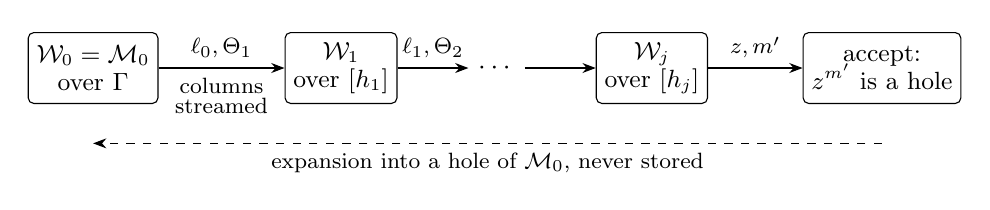
\begin{tikzpicture}[>=Stealth,
    mon/.style={draw, rounded corners=2pt, align=center, font=\small,
      inner sep=3pt, minimum height=9mm}]
  \node[mon] (w0) {$\mathcal W_0=\mathcal M_0$\\[-1pt]over $\Gamma$};
  \node[mon, right=16mm of w0] (w1) {$\mathcal W_1$\\[-1pt]over $[h_1]$};
  \node[right=9mm of w1] (dots) {$\cdots$};
  \node[mon, right=9mm of dots] (wj) {$\mathcal W_j$\\[-1pt]over $[h_j]$};
  \node[mon, right=12mm of wj] (acc) {accept:\\[-1pt]$z^{m'}$ is a hole};
  \draw[->] (w0) -- node[above,font=\footnotesize] {$\ell_0,\Theta_1$}
    node[below,font=\footnotesize,align=center] {columns\\[-2pt]streamed} (w1);
  \draw[->] (w1) -- node[above,font=\footnotesize] {$\ell_1,\Theta_2$} (dots);
  \draw[->] (dots) -- (wj);
  \draw[->] (wj) -- node[above,font=\footnotesize] {$z,m'$} (acc);
  \draw[->, dashed] ([yshift=-5mm]acc.south) -- node[below,font=\footnotesize]
    {expansion into a hole of $\mathcal M_0$, never stored}
    ([yshift=-5mm]w0.south);
\end{tikzpicture}
\caption{The summary search builds the derived monitors bottom-up. A derive
step chooses a marker $\ell_j$ of the current monitor $\mathcal W_j$, streams
the columns of $h_{j+1}$ distinct blocks that avoid it, keeps only their
summary $\Theta_{j+1}$, and moves to
$\mathcal W_{j+1}=\mathcal W_j[\ell_j,\Theta_{j+1}]$ over the abstract
letters $[h_{j+1}]$. Expanding the abstract letters level by level would
turn an accepted unary word into a hole of $\mathcal M_0$ (dashed arrow).
Compression in \cref{sec:search} instead starts from a given hole and
shortens its hierarchy top-down.}
\Description{A chain of current monitors from the original monitor to a level at which a unary word is accepted, with a dashed arrow back indicating the expansion into a hole that is never stored.}
\label{fig:summary-levels}
\end{figure}

\begin{proposition}[Summary search]\label{prop:summary-search}
Let $\mathcal M_0$ be a lettered monitor with $N\ge1$ states over a finite
alphabet $\Gamma$, given by its tables, and let $d\ge0$. Whether
$\mathcal M_0$ has a nonempty hole of depth at most $d$ is decidable in
nondeterministic space
\[
 O\bigl((N+d+1)^2\,(\DictBound(N,d)+|\Gamma|)^2\bigr),
\]
which is polynomial in $N+d+1$, the dictionary bound $\DictBound(N,d)$ of
\eqref{eq:dictionary-constants}, and $|\Gamma|$. Hence it is decidable in
deterministic space $2^{O((N+d+1)^3)}\cdot(1+|\Gamma|)^4$.
\end{proposition}

The search of \cref{fig:summary-search} has two moves. An accept move tests
a bounded unary hole of the current monitor. A derive move chooses a marker
and streams a bounded tuple of blocks that avoid it. The search maintains
the following invariant. At each level $j\ge1$, each current letter names a
distinct block over the letters of level $j-1$. The stored tables give the
transitions, final targets, and admissions of the corresponding derived
monitor on these letters. A derive move generates the blocks one column at a
time, checks from the equality bits of the summary that they are distinct,
and then retains only their names $1,\ldots,h$ and the tables of
$\mathcal W[\ell,\Theta]$. Higher levels use only this information.

An accepting computation could be expanded backward into a hole of
$\mathcal M_0$: replace each abstract letter by the block it names, level by
level, and close each block with its marker. Agreement
(\cref{lem:agreement-derivative}) and desubstitution (\cref{lem:der-holes})
make each expansion a hole of the monitor one level below, which gives
soundness; the search itself never performs or stores this expansion.
Completeness follows from the dictionary bound (\cref{lem:dictionary-bound}),
column shortening, and unary shortening (\cref{app:search}): the markers and
the shortened blocks of a suitable hole provide the guesses. The largest
stored items are the relations of the current monitor, the derived-admission
bits of one summary, and the column counter, each of
$O((N+d+1)^2(\DictBound(N,d)+|\Gamma|)^2)$ bits. The deterministic bound then
follows from Savitch's theorem~\citep{Savitch70}. The full proof is in
\cref{app:complexity}.

\begin{theorem}[Upper bounds]\label{thm:complexity}\label{cor:complexity}
For every arity $n$, every variance $c$, and each of the three tree domains,
entailment $\phi\models_{\mathcal D,c}x\le y$ of a flat system with $k$
variables is decidable in deterministic space
$2^{2^{O(k)}}\cdot\operatorname{poly}(\insize\phi)$. Hence entailment and
non-entailment are in 2-EXPSPACE and in 3-EXPTIME in each domain, also for
the general input syntax of \cref{prop:flattening}.
\end{theorem}

\begin{proof}[Proof sketch]
By \cref{lem:poly-tests}, decide in polynomial time whether $\phi$ is
satisfiable in $\mathcal D$; if it is not, the entailment holds. Otherwise,
by \cref{prop:transfer}, \eqref{eq:g13}, and \cref{thm:holes}, the entailment
holds iff neither label reader has a hole. The empty word is a hole iff the
initial state is rejected. By \cref{thm:brt,thm:depth}, a label reader has a
hole iff the empty word is a hole or the reader has a nonempty hole of depth
at most $d=8N^2-2N-1$. Its nonempty holes are those of its lettered monitor,
whose tables are computed entry by entry by \cref{lem:poly-tests}.
\Cref{prop:summary-search}, with $|\Gamma|=n$ and
$N+d+1=8N^2-N\le2^{8k+5}$, decides this in space $2^{2^{O(k)}}(1+n)^4$.
Since $k\le\insize\phi$, the whole procedure runs in space
$2^{2^{O(k)}}\operatorname{poly}(\insize\phi)$, hence in time
$2^{2^{2^{O(\insize\phi)}}}$. At positive arity, \cref{prop:flattening}
reduces the general syntax in polynomial time to a flat system with
$O(\insize\phi)$ variables; at arity zero, \cref{prop:arity-zero} in
\cref{app:small-arity} applies.
\Cref{app:complexity} gives the full accounting.
\end{proof}

\paragraph{Comparison with the Length Bound}
Guessing a hole of length at most $H$ and checking it places non-entailment
in 3-NEXPTIME and entailment in co-3-NEXPTIME, hence in 3-EXPSPACE; these are
the bounds that the length bound alone provides. \Cref{thm:complexity}
implies them, since
\[
 \text{2-EXPSPACE}\subseteq\text{3-EXPTIME}\subseteq
 \text{3-NEXPTIME}\cap\text{co-3-NEXPTIME},
\]
and it lowers the space bound by one exponential; by the space hierarchy
theorem \citep[Theorem~6]{StearnsHartmanisLewis65}, 2-EXPSPACE is a proper
subclass of 3-EXPSPACE. The bound $H$ on the hole length is unchanged. The
saving comes from representing one level of the hierarchy by the tables of
its derived monitor instead of storing a hole. For fixed $n\ge2$:
\begin{center}
\small
\begin{tabular}{@{}lll@{}}
\toprule
Procedure & Stored object & Resulting bound\\
\midrule
Enumeration (\cref{fig:algorithm}) & a word of length at most $H$ & time: four exponentials in $k$\\
Guessing a hole & a hole of length at most $H$ & 3-NEXPTIME, hence 3-EXPSPACE\\
Summary search (\cref{prop:summary-search}) & tables of one level & 2-EXPSPACE and 3-EXPTIME\\
\bottomrule
\end{tabular}
\end{center}
The search keeps tables of doubly exponential size in $k$, whereas the only
known bound on the hole length is triply exponential.

% complexity-lower: exponential holes and PSPACE-hardness for arity n >= 2

\subsection{Lower Bounds}
\label{sec:complexity-lower}

We prove two lower bounds for a covariant constructor of arity $n\ge2$:
holes can be forced to be exponentially long in $k$, and entailment is
PSPACE-hard, in each of the three domains.
All systems in this subsection are covariant, so $H_0$ is the identity in
\eqref{eq:g12}. A word $w$ is then left unsafe for $(\phi,x,y)$ iff some
solution $\sigma$ has $\widehat{\sigma(x)}(w)=\top\ne\widehat{\sigma(y)}(w)$,
and right unsafe iff some solution has
$\widehat{\sigma(y)}(w)=\bot\ne\widehat{\sigma(x)}(w)$. Proofs omitted here
are given in \cref{app:lower}.

\paragraph{Overview}
Both constructions simulate a nondeterministic automaton over $\{0,1\}$ by
constructor literals along binary paths. For long holes, lower literals run
an automaton on $y$: a transition $q\xrightarrow{a}q'$ places the $a$-child
of $Y_q$ above $Y_{q'}$, so $Y_q$ has no bottom prefix along any word that
the automaton accepts from $q$. All states of the automaton are final, so
its language is prefix closed, and the remaining words form a union of sets
$u\{0,1\}^*$. We use an automaton that accepts every word except the
extensions of one exponentially long word, the record of a binary counter.
Separate upper literals keep $x$ top free, with constructor positions in
$\{0,1\}^*$, so every unsafe word is right unsafe and extends the counter
record. Truncating the trees of the automaton states, with top leaves at a
depth beyond a chosen word, gives finite solutions, so these words are
unsafe in all three domains. For hardness the roles of the two kinds of
literals are reversed: upper literals run a given automaton on $x$, and lower
literals keep a second variable $r$ at least a constructor along every
proper prefix of a code word.

\paragraph{Constructor Positions}
For a tree $t$, let $\Pos(t)=\{w\in\operatorname{dom}(t):t(w)=f\}$ be its
set of \emph{constructor positions}; it is prefix closed. A tree is
\emph{top free} if no node is labeled $\top$. Every prefix-closed set
$P\subseteq\Dir^*$ is $\Pos(T_P)$ for exactly one top-free tree $T_P$: its
domain is $\{\eps\}\cup P\cup P\Dir$, its label is $f$ on $P$, and $\bot$
elsewhere. For example, $T_\varnothing=\Bot$, and $T_{\{0,1\}^*}$ is the
full constructor tree $F$ when $n=2$. For a prefix-closed set $P$ and
$m\ge1$, the \emph{truncation} $T_P^m$ is obtained from $T_P$ by replacing the
subtree at every word of $P$ of length $m$ by $\Top$; it is a finite tree.
For variables $a_0,a_1,b$ we write $f(a_0,a_1,\bar b)$ for
$f(a_0,a_1,b,\ldots,b)$, with $n-2$ copies of $b$; for $n=2$ it stands for
$f(a_0,a_1)$.

\begin{lemma}[Top-free trees]\label{lem:cx-topfree}
Let $n\ge2$.
\begin{enumerate}[leftmargin=*]
\item For top-free trees $t,u$ and every word $w$, $\widehat t(w)=f$ if
  $w\in\Pos(t)$ and $\widehat t(w)=\bot$ otherwise; and $t\le u$ iff
  $\Pos(t)\subseteq\Pos(u)$.
\item $T_P$ is finite iff $P$ is finite.
\item Let $\sigma$ satisfy $b=\Bot$ and $g\le f(g,g,\bar b)$. Then
  $\sigma(g)$ is top free and $\Pos(\sigma(g))\subseteq\{0,1\}^*$, and so is
  every tree $t\le f(\sigma(g),\sigma(g),\Bot,\ldots,\Bot)$.
\item Let $P,P'$ be prefix closed, $\eps\in P$, $a\in\Dir$, and
  $aP'\subseteq P$. Then $f(t_0,\ldots,t_{n-1})\le T_P^m$ for every $m\ge1$,
  where $t_a=T_{P'}^m$ and $t_i=\Bot$ for $i\ne a$.
\end{enumerate}
\end{lemma}

Item~(3) holds because a top leaf cannot lie below a constructor: by
\eqref{eq:g11}, a top leaf of $\sigma(g)$ at a word $iw$ would force
$i\in\{0,1\}$ and a top leaf at the shorter word $w$, and $\sigma(g)$ has no
top leaf at $\eps$. In item~(4), the truncation at the same depth $m$ on both
sides is what makes the inequality hold: a top leaf of $T_{P'}^m$ at a word
$v$ of length $m$ lies below the top leaf of $T_P^m$ at the prefix of $av$ of
length $m$.

\paragraph{Long Holes}
As noted in \cref{sec:complexity-upper}, a failed entailment on a
satisfiable system is certified by a hole of one of the two label readers,
and by \cref{thm:holes} these holes are exactly the unsafe words. Such
certificates can be forced to be exponentially long. The construction uses
an automaton with $O(\beta)$ states for the binary words that do not begin
with one word of length $2(\beta+1)2^\beta$, the record of a $\beta$-bit
binary counter.

Fix $\beta\ge1$. Over the \emph{token alphabet} $\mathbb T=\{0,1,\#,\$\}$,
let $\cxbin j$ be the binary expansion of $j$ with $\beta$ bits, least
significant bit first, and put
\[
 \mathsf H_\beta=\cxbin0\#\cxbin1\#\cdots\#\cxbin{2^\beta-1}\$,
 \qquad \len{\mathsf H_\beta}=(\beta+1)2^\beta.
\]
The \emph{token encoding} maps the letters of $\mathbb T$ to $0\mapsto00$,
$1\mapsto01$, $\#\mapsto10$, and $\$\mapsto11$. Let
$\mathsf W_\beta\in\{0,1\}^*$ be the token encoding of $\mathsf H_\beta$, of
length $\lambda_\beta=2(\beta+1)2^\beta$. For $\beta=1$,
$\mathsf H_1=0\#1\$$ and $\mathsf W_1=00100111$. In a nondeterministic
automaton all of whose states are final, a word is accepted iff it has a
run, that is, a path labeled by the word from an initial state.

\begin{lemma}[Counter automaton]\label{lem:cx-counter}
For every $\beta\ge1$ there is a nondeterministic automaton $\mathcal B_\beta$
over $\{0,1\}$ with $9\beta+27$ states, all of them final, whose language is
$\{0,1\}^*\setminus\mathsf W_\beta\{0,1\}^*$. It is computable in time
polynomial in $\beta$.
\end{lemma}

The automaton reads the encoded tokens. In parallel, its branches check the
format of the blocks, that the first block is zero, that each block is the
successor of the previous one, and that $\$$ follows exactly the all-ones
block. A branch that detects an error enters a state that loops on every
letter, and on $\mathsf W_\beta$ itself every branch dies (\cref{app:lower}).
For instance, for $\beta=2$ the record is $\mathsf H_2=00\#10\#01\#11\$$. In a
token word that begins with $00\#10\#11$, the first bit of the third block is
wrong: the successor of $10$, that is, of $1$, is $01$. The branch spawned at
the first bit of the second block predicts the bit $0$ from that bit and the
carry, counts $\beta+1=3$ tokens, and reads $1$ instead. It detects the
error while storing only the predicted bit and a counter, not the history.

Let $Q$ be the set of states of $\mathcal B_\beta$, $I\subseteq Q$ its
initial states, and $q\xrightarrow{a}q'$ its transitions. Add a state
$q_{\mathrm{in}}$ with $q_{\mathrm{in}}\xrightarrow{a}q'$ iff
$q\xrightarrow{a}q'$ for some $q\in I$, so that $q_{\mathrm{in}}$ accepts the
language of $\mathcal B_\beta$. For $n\ge2$, let $\Phi_\beta^{(n)}$ have the
variables $x$, $g$, $b$, and $Y_q$ for $q\in Q\cup\{q_{\mathrm{in}}\}$, with
$y=Y_{q_{\mathrm{in}}}$, and the flat literals
\[
\begin{aligned}
 &b=\Bot,\quad g\le f(g,g,\bar b),\quad x\le f(g,g,\bar b)
   &&\text{(confinement to binary paths)},\\
 &f(b,b,\bar b)\le Y_q &&\text{(nonbottom roots)},\\
 &f(Y_{q'},b,\bar b)\le Y_q\ \ (q\xrightarrow0q'),\quad
  f(b,Y_{q'},\bar b)\le Y_q\ \ (q\xrightarrow1q')
   &&\text{(propagation along transitions)},
\end{aligned}
\]
for all $q\in Q\cup\{q_{\mathrm{in}}\}$. Thus $y$ receives the lower literals
of the initial states directly. Write $\Phi_\beta=\Phi_\beta^{(2)}$. For every
$n$, $\Phi_\beta^{(n)}$ has $k=9\beta+31$ variables. The confining literals
keep $x$ top free, with constructor positions in $\{0,1\}^*$. The other two
groups give each $Y_q$ a constructor or a top prefix along every word that
$\mathcal B_\beta$ accepts from $q$, so $y$ has no bottom prefix along any
binary word without the prefix $\mathsf W_\beta$. The trees of $y$ and of the $Y_q$
may have top leaves, which permits finite solutions.

\begin{proposition}[Exponentially long holes]\label{prop:cx-length}
Let $n\ge2$, let $f$ be covariant of arity $n$, let $\beta\ge1$, and let
$\Phi=\Phi_\beta^{(n)}$, with the query $x\le y$.
\begin{enumerate}[leftmargin=*]
\item $\Phi$ has a finite solution, and $\Phi\models_{\mathcal D}x\le y$ fails
  in each of the three domains $\mathcal D$.
\item No word is left unsafe, and the right-unsafe words are exactly the
  words of $\mathsf W_\beta\{0,1\}^*$.
\item The left label reader
  $(\mathcal M_{\mathsf l},\Adm_{\mathsf l},\Rej_{\mathsf l})$ has no hole,
  and the holes of the right label reader
  $(\mathcal M_{\mathsf r},\Adm_{\mathsf r},\Rej_{\mathsf r})$ are exactly the
  words of $\mathsf W_\beta\{0,1\}^*$. In particular, every hole that the
  search of \cref{fig:algorithm} can find has length at least
  $\lambda_\beta=2(\beta+1)2^\beta$, and $\mathsf W_\beta$ is a hole of this
  length.
\end{enumerate}
Hence, for every fixed arity $n\ge2$ and in each domain, shortest holes of
systems with $k$ variables can have length $2^{\Omega(k)}$: here
$\lambda_\beta\ge2^{(k-22)/9}$.
\end{proposition}

\begin{proof}[Proof idea]
For $n=2$, let $\sigma$ be a solution. By \cref{lem:cx-topfree}(3), $\sigma(x)$
is top free with $\Pos(\sigma(x))\subseteq\{0,1\}^*$, so no word is left
unsafe, and a right-unsafe word $w$ has $w\in\Pos(\sigma(x))$ and
$\widehat{\sigma(y)}(w)=\bot$ for some solution $\sigma$. Induction along runs of
$\mathcal B_\beta$ shows that $\widehat{\sigma(y)}$ is not $\bot$ on the language
of $\mathcal B_\beta$, so by \cref{lem:cx-counter} every right-unsafe word
begins with $\mathsf W_\beta$. Conversely, let $w\in\mathsf W_\beta\{0,1\}^*$
and $m=\len w+1$. The truncations $Y_q=T_{L_q}^m$, with $L_q$ the set of words
accepted from $q$, together with $g=T_{\{0,1\}^{<m}}$, $b=\Bot$, and $x=T_P$ for
the set $P$ of prefixes of $w$, form a finite solution with $w\in\Pos(x)$ and
$\widehat y(w)=\bot$ (\cref{lem:cx-topfree}(4)). This gives~(1) and~(2),
and~(3) follows by \cref{thm:holes}. The case $n\ge3$ reduces to $n=2$ by an
embedding of binary trees, described at the end of this subsection. The
details are in \cref{app:lower}.
\end{proof}

Since $N=2^{4k+1}$, the length $\lambda_\beta$ is only polynomial in $N$,
whereas the length bound $H$ of \cref{sec:complexity-upper} is triply
exponential in $k$.

\paragraph{Hardness}
\Citet[Theorems~1 and~2]{HengleinRehof98} proved PSPACE-hardness for a binary
covariant constructor over arbitrary and over finite trees
(\cref{sec:related}). We give a reduction from universality of
nondeterministic automata over $\{0,1\}$ that works in all three domains and
for every fixed arity $n\ge2$. An automaton $\mathcal A=(Q,q_0,F,\delta)$ has
one initial state $q_0$, final states $F$, and transitions
$\delta\subseteq Q\times\{0,1\}\times Q$; it is universal if it accepts every
word. Universality of such automata is PSPACE-hard.\footnote{%
\citet[Theorem~3]{KrotzschMasopustThomazo16} prove this for automata over
$\{0,1\}$, even for partially ordered ones. Their automata may have several
initial states; a fresh initial state that has the outgoing transitions of
all of them, and is final iff one of them is, accepts the same language. For
regular expressions over $\{0,1\}$ with union, concatenation, and star, the
classical result is due to \citet[Section~3]{StockmeyerMeyer73}, who state
that inequivalence is complete for nondeterministic linear space.}

The reduction runs an automaton on $x$ by upper literals, and an accepting
run forces the subtree of $x$ at its end to be $\Bot$; then $x$ has no node
below that word. A word at which $x$ is to have a constructor while a second
variable $r$ is $\bot$ must therefore have no accepted prefix. We encode
words by a prefix-free code, so that the code of a rejected word has no
accepted code as a prefix. The variables $r$ and $r'$ track the position
within an encoded letter (\cref{fig:cx-code}). Their lower literals keep $r$
at least a constructor at every proper prefix of a code, while at a
completed code $r$ may be $\bot$, where $x$ can still have a constructor if
the code is rejected.

For $w\in\{0,1\}^*$ let $\cxcode(w)=e(w)1$, where $e$ replaces each letter
$0$ by $00$ and each $1$ by $01$; we call $\cxcode$ the \emph{prefix-free
code}. On single bits, $e$ agrees with the token encoding, but the two
encodings serve different constructions. The code is prefix
free: if $\cxcode(w')\pre\cxcode(w)$ and $\len{w'}<\len w$, then position
$2\len{w'}$ carries the final $1$ of $\cxcode(w')$ but the letter $0$ in
$\cxcode(w)$. From $\mathcal A$ we obtain in linear time an automaton
$\mathcal A'$, again with the initial state $q_0$, that accepts
$\cxcode(L(\mathcal A))$: replace each transition $(q,a,q')$ by
$q\xrightarrow0\mu\xrightarrow{a}q'$ through a new middle state $\mu$, and
add a transition labeled $1$ from every final state to one new state
$q_{\mathrm f}$, the only final state of $\mathcal A'$.

For such an automaton $\mathcal A'$ with states $Q'$, let $\chi(\mathcal A')$
have the variables $z$, $b$, $r$, $r'$, and $X_q$ for $q\in Q'$, write $x$ for
$X_{q_0}$, and take the flat literals
\[
\begin{gathered}
 X_q\le f(X_{q'},z,b,\ldots,b)\ \ (q\xrightarrow0q'),\qquad
 X_q\le f(z,X_{q'},b,\ldots,b)\ \ (q\xrightarrow1q'),\qquad
 X_{q_{\mathrm f}}=\Bot,\\
 b=\Bot,\qquad f(r',b,\ldots,b)\le r,\qquad f(r,r,b,\ldots,b)\le r'.
\end{gathered}
\]
Here $b$ fills the arguments $2,\ldots,n-1$ of the first two literals and
the arguments $1,\ldots,n-1$ of the first lower literal; for $n=2$ the first
two literals have no $b$. No literal bounds $z$, so $z$ may be $\top$, and
then, among the two binary children, an upper literal constrains only the child
that the run follows; the added children are bounded by $b=\Bot$. Along
every run of $\mathcal A'$ from $q_0$ on a word $u$, the upper literals keep the subtree
of $x$ at $u$, if it exists, below the variable $X_q$ of the reached state
$q$; an accepting run therefore forces the subtree of $x$ at its end, if it
exists, to be $\Bot$. The lower literals give $r$ a constructor or $\top$ at
every proper prefix of a code, and they allow $r$ to be $\bot$ at a code. If
$\mathcal A$ is universal, every proper prefix of a code lies on an accepting
run, and $x\le r$ follows. If $\mathcal A$ rejects a word $w$, then a solution
can give $x$ a constructor at $\cxcode(w)$ and $r$ the label $\bot$ there.

\begin{figure}[tbp]
\centering
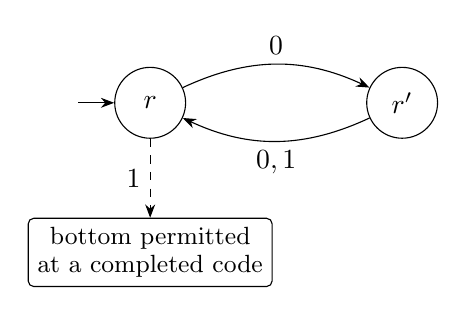
\begin{tikzpicture}[>=Stealth, auto,
    every state/.style={minimum size=9mm, inner sep=1pt}]
  \node[state, initial, initial text={}] (r) at (0,0) {$r$};
  \node[state] (rp) at (3.2,0) {$r'$};
  \node[draw, rounded corners=2pt, font=\small, align=center] (bot) at (0,-1.9)
    {bottom permitted\\[-1pt]at a completed code};
  \draw[->] (r) edge[bend left=25] node {$0$} (rp);
  \draw[->] (rp) edge[bend left=25] node {$0,1$} (r);
  \draw[->, dashed] (r) -- node[left] {$1$} (bot);
\end{tikzpicture}
\caption{The lower literals $f(r',b,\ldots,b)\le r$ and
$f(r,r,b,\ldots,b)\le r'$ of $\chi(\mathcal A')$ as a diagram: an edge
labeled $a$ from $v$ to $v'$ means that the $a$-child of $v$ lies above $v'$.
Reading the encoding $e(w)$ of a word follows the solid edges, so the tree
of $r$ has a constructor or $\top$ at every proper prefix of a code. The
final $1$ of $\cxcode(w)$ leaves the diagram (dashed): at a completed code the
tree of $r$ may have the label $\Bot$, although $r$ itself is never $\Bot$.}
\Description{Two states r and r prime with a 0-edge from r to r prime and a 0,1-edge back, and a dashed 1-edge from r to a box saying that the tree of r may be bottom at a completed code.}
\label{fig:cx-code}
\end{figure}

\begin{theorem}[PSPACE-hardness]\label{thm:cx-hard}
Let $n\ge2$ be fixed and let $f$ be covariant. For every automaton
$\mathcal A$ over $\{0,1\}$ and each domain $\mathcal D$,
\[
 \chi(\mathcal A')\models_{\mathcal D}x\le r
 \quad\Longleftrightarrow\quad
 \mathcal A\text{ is universal}.
\]
Consequently, in each of the three domains, entailment of flat systems over
$\{\Bot,f,\Top\}$ is PSPACE-hard. So is the problem with the variance as part
of the input, already on covariant instances.
\end{theorem}

\begin{proof}[Proof idea]
Let $P$ be the set of proper prefixes of codes, the words $e(w)$ and
$e(w)0$. If $\mathcal A$ is universal, every word of $P$ lies on an accepting
run of $\mathcal A'$, so in every solution the subtree of $x$ there, if
present, lies below a constructor tree whose arguments $2,\ldots,n-1$ are
$\Bot$; every code is accepted, so $x$ is $\Bot$ at codes. Along $P$, the
lower literals give $r$ only the labels $f$ and $\top$. Every common position
of $x$ and $r$ therefore compares a label at most $f$ with one at least $f$,
or has $x=\Bot$. If $\mathcal A$ rejects $w$, no prefix of $\cxcode(w)$ is
accepted by $\mathcal A'$, and a path tree along $\cxcode(w)$ together with
finite approximants of $r$ forms a finite countermodel, which lies in every
domain. The system is satisfiable, has $\len{Q'}+4$ variables, and is
computed in polynomial time. The details are in \cref{app:lower}.
\end{proof}

For $n=2$ and arbitrary or finite trees, \cref{thm:cx-hard} reproves, by a
different reduction, the hardness theorems of
\citet[Theorems~1 and~2]{HengleinRehof98}, which are stated for a binary
covariant constructor over these two domains. It gives a uniform proof for
all three domains and every fixed arity $n\ge2$. Their theorems do not state
the regular case, and we do not claim that it is new. We claim no hardness
for a fixed variance with a contravariant argument, nor for arity one
(\cref{app:small-arity}).

\paragraph{Larger Arities}
The hardness reduction works directly at every arity $n\ge2$. The systems
$\Phi_\beta^{(n)}$ for long holes are obtained from $\Phi_\beta$ by filling
the new arguments of every constructor with the variable $b=\Bot$. Such
\emph{bare padding} does not preserve lower bounds in general. The padded
system also constrains trees that are not images of binary trees, and these
may refute the entailment at short words that use the new letters.

\begin{example}[Bare padding fails]\label{ex:cx-padding}
For a binary covariant $f_2$, the system
\[
 \chi=\{x\le f_2(y,b),\ f_2(z,b)\le y,\ f_2(z,t)\le z,\ b=\Bot,\ t=\Top\}
\]
entails $x\le y$. Indeed, every top leaf of $x$ lies at a word $0v$ such that
$y$ has a top prefix along $v$. Then $y$ also has one along $0v$: either
$y=\Top$, or the child $0$ of $y$ lies above $z$, which has a top prefix along
every word that begins with $0^j1$; and for $v\in0^*$, the top prefix along
$v$ lies along $0v$. Moreover, $y$ has bottom prefixes only along words that
begin with $1$, where $x$ has one as well. Padding with a variable $o=\Bot$
in the third argument, for $n=3$, loses the entailment: the finite assignment
$x=f(f(\Bot,\Bot,\Top),\Bot,\Bot)$, $y=f(z,\Bot,\Top)$, $z=f(\Top,\Top,\Bot)$,
$b=o=\Bot$, and $t=\Top$ is a countermodel, since $x$ has a top leaf at $02$,
where $y$ has the bottom leaf of $z$.
\end{example}

Padding with $\Bot$ does preserve solutions and unsafe words on binary
paths: lifting a binary tree by adding $\Bot$ children, and projecting a tree
over $\Dir$ to its binary paths, map solutions to solutions in each domain
and keep leaf extensions on $\{0,1\}^*$ (\cref{prop:cx-embedding} in
\cref{app:lower}). For $\Phi_\beta^{(n)}$, the confining literals
$g\le f(g,g,\bar b)$ and $x\le f(g,g,\bar b)$ also exclude unsafe words that
use an added child position, because they keep $x$ top free with constructor
positions in $\{0,1\}^*$. Thus $\Phi_\beta^{(n)}$ and $\Phi_\beta$ have
exactly the same unsafe words. The system of \cref{ex:cx-padding} has no
confining literals, and the word $02$ of its countermodel is left unsafe and
uses the added letter $2$. The embedding is therefore not a general
reduction between arities, such as the equivalence of all arities at least
two asserted by \citet[Corollary~1]{NiehrenPriesnitz03} (\cref{sec:errata}).
It transfers unsafe words only on binary paths, which suffices when
confining literals exclude all other words.

\paragraph{Combined Bounds}
Together with \cref{thm:complexity}, entailment for a covariant constructor
of each fixed arity $n\ge2$ is PSPACE-hard and in 2-EXPSPACE in each domain.
\Cref{sec:future} discusses the open questions about its exact complexity.


\section{Mechanization}
\label{sec:mechanization}

The artifact, a development in Lean~4 \citep{MouraUllrich21} with Mathlib
\citep{Mathlib20}, contains decision procedures for all three domains that
search for holes in three ways: by bounded enumeration
(\cref{fig:algorithm}), by the summary search of
\cref{sec:complexity-upper}, and, at arity one, by the single-word test of
\cref{app:small-arity}. Their correctness is mechanized end to end for flat
constraints. The development covers arbitrary arity and variance, signed
constraints, satisfiability, the semantic reduction, the alphabet-generic
hole bounds, and both domain transfers. The hole-bound modules include
isolated exchange, induced level maps, normal forms, boundary-pair
propagation, and compression within fixed original dictionaries. The
artifact also contains a certifying solver whose answers are checked by
proved checkers. Lean and Mathlib are both pinned to \texttt{v4.35.0}.

The trusted statement consists of the definitions of trees, the variance
order, flat constraints, satisfaction, and entailment in each domain.
A characterization module connects the path-based order to the greatest
fixed point of the constructor rule and shows that the finite and regular
representations denote the intended tree classes. The kernel checks the
proof terms establishing equivalence with finite search. The procedures
are computable definitions. The proof dependencies and commands for
checking them appear in \cref{app:lean-artifact}.

The final bounds are parameterized by the original reader-state count $N$,
without a preliminary state refinement. Tail and depth use those states
directly; compression uses derivative monitors with $N+j$ states at
level $j$, as accounted for in \eqref{eq:holebound}. The paper and artifact
have the same final bounds. Some intermediate statements and constants
differ; \cref{app:lean} gives the public API, module layout, correspondence,
and these differences. \lean{ElementaryBound.lengthBound} defines
$\holeBound(N,d)$; \lean{ElementaryBound.exists_short_hole} proves the
bounded-depth witness theorem. The back end uses
\lean{RejectedTail.holeLengthBound}, and
\lean{RejectedTail.holeLengthBound_le} proves the closed-form estimate
$H\le2^{2^{1280(N+1)^5}}$.

The module \texttt{Complexity} mechanizes the combinatorial content of
\cref{sec:complexity,app:small-arity}. The summary search is proved sound
and complete, and entailment procedures built on it are proved correct in
each domain. For the label readers,
\lean{Complexity.Summary.card_config_label_le} bounds the number of
configurations so that one configuration fits in
$2^{2^{O(k)}}\cdot\operatorname{poly}(n)$ bits, matching the space bound of
\cref{thm:complexity}; \cref{app:lean-complexity} states the exact bound.
Unlike the nondeterministic search of \cref{prop:summary-search}, which
counts the columns of a derive move to bound its space, the mechanized search
decides reachability of an accepting configuration in a finite graph and
keeps no column counter. The configuration bound supports the space
argument, but the executable search computes the reachable set by
saturation and is not proved to run in that space.
\lean{Complexity.Unary.exists_hole_length_le} proves the bound $N-1$ for every
reader over a one-letter alphabet, and the unary procedures test only the
word up to the first rejected cut. For every arity $n\ge2$ and each domain,
\lean{Complexity.entails_hardnessSystem_iff} and its regular and finite
versions prove the hardness reduction correct, with linearly many literals;
the systems of \cref{prop:cx-length} refute entailment, and
\lean{Complexity.expSystem_shortest_hole} gives their exact shortest hole
length $2(\beta+1)2^\beta$. Not mechanized are the complexity classes
themselves, that is, space-bounded machines, Savitch's theorem, and the
space hierarchy theorem; the PSPACE-hardness of universality; the
polynomial-time tests of \cref{lem:poly-tests}; and the polynomial-time
procedure at arity zero (\cref{prop:arity-zero}).
\Cref{app:lean-complexity} gives the correspondence and the differences.

The artifact is included in
\anon[the supplementary material]{\url{https://github.com/noti0na1/deci-nsse}}.
The NP03 counterexample is derived in full in \cref{app:np03}. A separate
kernel-checked formalization agrees with that argument and is not part
of this artifact.

\section{Related Work}
\label{sec:related}

\Cref{tab:results} summarizes selected results on subtype entailment.

\begin{table}[tbp]
\caption{Selected results on subtype entailment. Earlier non-structural rows concern a
covariant constructor; our decidability result allows arbitrary variance and arity.
The complexity bounds for our results are proved in \cref{sec:complexity};
\cref{sec:mechanization} states which parts of them are mechanized.}
\label{tab:results}
\small\setlength{\tabcolsep}{3pt}
\begin{tabular}{@{}>{\raggedright\arraybackslash}p{0.29\linewidth}>{\raggedright\arraybackslash}p{0.18\linewidth}>{\raggedright\arraybackslash}p{0.20\linewidth}>{\raggedright\arraybackslash}p{0.27\linewidth}@{}}
\toprule
Problem & Trees & Result & Reference \\
\midrule
Structural entailment & finite & coNP-complete & \citet{HengleinRehof97} \\
Structural entailment & arbitrary & PSPACE-complete & \citet{HengleinRehof98} \\
Structural, first-order theory & finite & decidable & \citet{KuncakRinard03} \\
\NSSE, $\ftree$ unary & finite, regular, arbitrary & decidable & \citet{NiehrenPriesnitz03} \\
\NSSE, $\ftree$ binary, no literals $x = \Bot$, $x = \Top$ & finite, arbitrary & PSPACE-complete & \citet{NiehrenPriesnitz99} \\
\NSSE, $\ftree$ binary & finite, arbitrary & PSPACE-hard & \citet[Theorems~1--2]{HengleinRehof98} \\
\NSSE, any arity and variance & finite, regular, arbitrary & decidable; in 2-EXPSPACE (stronger for $n\le1$, \cref{app:small-arity}) & this paper \\
\NSSE, $\ftree$ covariant, any fixed arity $n\ge2$ & finite, regular, arbitrary & PSPACE-hard & this paper \\
Non-structural, first-order theory & finite, regular, arbitrary & undecidable & \citet{SuAikenNiehrenPriesnitzTreinen02} \\
\bottomrule
\end{tabular}
\end{table}

\paragraph{Subtype Entailment and Constraint Simplification}
Subtype constraints arise in type inference with subtyping
\citep{Mitchell91,FuhMishra90,AikenWimmers93,EifrigSmithTrifonov95,PalsbergWandOKeefe97},
and the size of inferred constraint sets made simplification a central practical concern
\citep{Pottier96,Pottier98thesis,Pottier01,TrifonovSmith96}. Sound but incomplete
entailment tests based on syntactic closure are used in practice; \citet{Pottier01} discusses
their limits. Satisfiability of subtype
constraints is comparatively well understood
\citep{Tiuryn92,PrattTiuryn96,Frey97,KozenPalsbergSchwartzbach94,PalsbergOKeefe95,PalsbergWandOKeefe97,Simonet03,NiehrenPriesnitzSu05}.
Closure-based satisfiability characterizations are classical.
\citet{KozenPalsbergSchwartzbach94} treat a language with $\Top$ but
without $\Bot$; related characterizations appear in
\citet{PalsbergOKeefe95,PalsbergWandOKeefe97}.
Here the additional ingredients are a common least shape under variable flip
and polarity selection for variance. Subtyping between recursive types without variables
is also well understood
\citep{AmadioCardelli93,KozenPalsbergSchwartzbach95}. For entailment, \citet{HengleinRehof97} proved coNP-completeness for structural subtyping over
finite trees and \citet{HengleinRehof98} PSPACE-completeness over arbitrary trees. Their Theorems~1 and~2 establish
non-structural PSPACE-hardness using a binary covariant constructor, over
arbitrary and finite trees, respectively; this is the scope recorded in
\cref{tab:results}. \Cref{thm:cx-hard} gives a different reduction, from
universality of nondeterministic automata, with a uniform proof for all three
domains and every fixed arity $n\ge2$. \citet{Rehof97,Rehof98thesis} studies
minimal typings and the complexity of atomic and structural subtyping.
\citet{KuncakRinard03} show that the full first-order theory of structural subtyping of
non-recursive types is decidable.

\paragraph{Non-Structural Subtype Entailment}
\citet{NiehrenPriesnitz99} proved PSPACE-completeness for the fragment in which the
constraints contain no literals $x = \Bot$ and $x = \Top$ (the constants may still occur in
solutions), by a reduction to universality of finite automata; they introduced P-automata to
explain why the nonregular sets of paths that arise in general can be ignored in this
fragment. \citet{NiehrenPriesnitz01,NiehrenPriesnitz03} introduced cap
automata and cap set expressions, proved decidability of the unary case,
and identified the role of word equations in the general problem. Their
forward reduction from entailment to cap-automaton universality motivates
our use of periodic suffix comparisons. \Cref{sec:errata} discusses the
proof dependencies of their converse reduction and arity equivalence.
Priesnitz's theses \citep{Priesnitz00,Priesnitz04} develop the automata
approach further.
\citet{SuAikenNiehrenPriesnitzTreinen02} proved that the first-order theory
of non-structural subtyping is undecidable. This does not settle entailment,
which is a restricted universal implication. They and \citet{Su02} also
proposed a reduction of entailment to constrained tree automata on tuples of
trees, whose emptiness problem is undecidable in general \citep{Treinen00};
an extended version of the paper develops this reduction further
\citep{SuEtAl06}. A preprint
claimed membership in PSPACE for the finite and regular cases \citep{Schubert21}; it was
withdrawn by its author because of an error in a key lemma. The
problem has been described as open in work on intersection types and on type inference
\citep{DudenhefnerMartensRehof17,JiangCuiOliveira25}.

\subsection{The Published Characterization}
\label{sec:errata}
Proposition~16 of NP03 is false as stated:
\cref{app:np03} gives a six-state complete restricted cap automaton that
rejects $11$, whereas the left automaton of its back-translated judgment
accepts $11$ under either finality convention for Table~3. The judgment
is moreover a satisfiable entailment. Theorem~4 and the converse
reduction underlying Theorem~1 rely on Proposition~16.
Corollary~1 (equivalence of arities at least two and of tree classes)
also relies on that converse, and its arity part on Proposition~17.
Theorem~4, Theorem~1, and Corollary~1 themselves are not refuted;
only their published proofs are incomplete. No defect in Proposition~17
is claimed here. The forward characterization
(Theorem~2, with Propositions~8 and~11) is unaffected: it is
all that NP03's unary decidability result and the earlier binary proof
in \cref{sec:earlier} use.
The proofs of Propositions~12 and~14 treat states ready by the bottom,
top, or reflexivity rule as final. Table~3 must be read with that
convention: read literally, it rejects the path $1$ of NP03's unary
example $\judg{z=\Top\wedge f(z)\le y}{x}{y}$ (Section~4), which NP03
shows to be both left safe and right safe. \Cref{app:np03} gives the
acceptance details.
Our present proof uses neither the forward characterization nor any of
these converse or alphabet reductions.

\subsection{Other Connections}
\paragraph{Set Constraints and Feature Trees}
Entailment has been studied for neighboring constraint languages. Entailment of atomic set
constraints is PSPACE-complete over infinite signatures \citep{NiehrenMullerTalbot99}.
Ordering constraints over feature trees admit efficient entailment tests under an
assumption of infinitely many features \citep{MullerNiehrenPodelski00}, while their full
first-order theory is undecidable \citep{MullerNiehrenTreinen98}. Componential set-based
analysis uses entailment of set constraints for simplification \citep{FlanaganFelleisen99}.

\paragraph{Type Inference Without General Entailment}
Several modern approaches to type inference with subtyping avoid general entailment by
changing the type language or the semantics. Algebraic subtyping
\citep{Dolan16,DolanMycroft17,Parreaux20} interprets types in an algebraic model rather than
as ground trees, and infers principal types by biunification on polarized types, treating
subsumption between inferred types separately. MLstruct extends this approach to a Boolean
algebra of structural types \citep{ParreauxChau22}, and \citet{ParreauxEtAl24} retain
subtyping constraints in polymorphic types. Semantic subtyping interprets types as sets of
values and decides subtyping between types, including with polymorphism
\citep{CastagnaXu11,GesbertGenevesLayaida15}. Orthologic type systems obtain efficient
entailment for an open-world semantics \citep{GuilloudKuncak25}. These approaches use different type languages or semantic models, so their
decidability results do not directly decide the ground-tree entailment
problem studied here.

\paragraph{Word Equations and Periodicity}
Satisfiability of word equations is decidable \citep{Makanin77} and in PSPACE
\citep{Plandowski04}, but the positive $\forall\exists^3$ fragment is undecidable
\citep{Durnev95}. \citet[Corollary~2]{NiehrenPriesnitz03} express \NSSE in the positive
$\forall\exists^*$ fragment with regular constraints. Existential word-equation algorithms do not
directly decide this quantified formulation. Undecidability of the ambient
fragment leaves open the restricted instances arising from \NSSE, which
our reader construction and compression argument decide.
The periodicity arguments use the principle that sufficiently long agreement
between two periods forces agreement between their residue classes
\citep{FineWilf65}. \Cref{lem:rotation} proves the special case it needs
directly, and in \cref{lem:truncation}, equality over one full period
propagates along the periodic tail. These are instances of classical
periodic-word reasoning \citep{Lothaire02}, without a general word-equation
algorithm.

\paragraph{Back-References}
A cap repeats a root word that is chosen during the run, which resembles a back-reference in
an extended regular expression. For extended regular expressions, universality is
undecidable even with a single variable \citep{Freydenberger11}. Cap set expressions are a
much weaker mechanism: the only repetition is the prefix closure of the powers of one word,
and that word must be followed to the end of the path. Even so, universality of unrestricted
cap automata was left open by \citet[Section~10]{NiehrenPriesnitz03};
our decision procedure applies to readers satisfying the rejected-path property
and does not settle that question.

\paragraph{Desubstitution}
Cutting a sequence at the occurrences of a word and recoding the blocks between them is the
idea behind \emph{return words} and \emph{derived sequences} in symbolic dynamics
\citep{Durand98}, and the question whether such decompositions are unique is the subject of
recognizability theory \citep{Mosse92}. Our hierarchy cuts a finite word at its last letter,
and \cref{lem:cores} identifies the retained positions with the occurrences of a terminal
word. The connection is the recoding of intervals between repeated
occurrences. Here the chosen marker directly delimits the blocks, so unique
parsing needs no recognizability theorem. We use the hierarchy as a measure of the
complexity of a hole whose levels can be bounded (\cref{thm:depth}) and compressed
(\cref{thm:search}).

\paragraph{Automata with Constraints}
Our problem resembles emptiness for automata with equality and disequality constraints, where
pumping must preserve the constraints. For tree automata with constraints between brothers
\citep{BogaertTison92}, reduction automata \citep{DauchetCaronCoquide95}, and global constraints
\citep{TATA,ComonJacquemard03,FiliotTalbotTison10,BargunoEtAl10}, emptiness proofs replace
subterms \emph{simultaneously} while preserving states and equality patterns, rather than
pumping one subterm at a time. The column summaries of \cref{sec:search} follow the same
principle for the blocks of one hierarchy level. The new difficulty in \NSSE is that the
constraints compare suffixes of a single word at unbounded offsets; the admission cone
and the depth bound are what reduce it to a setting where simultaneous replacement suffices.

\section{From the Binary Proof to the General Proof}
\label{sec:experience}

An earlier version of this work treated only the binary covariant signature,
through cap automata. The present proof constructs readers directly from
subtype constraints and handles arbitrary arity and variance. This section
explains the change. \Cref{app:history} lists the distinctions on which both
proofs rely, with the places where the present proof handles them.

\subsection{An Earlier Proof for the Binary Covariant Case}
\label{sec:earlier}
The earlier version decided \NSSE for the binary covariant interpretation
of the TLCA problem, over the same three domains. It was based on the
\emph{cap automata} of \citet{NiehrenPriesnitz03}: finite automata with
additional \emph{P-edges}. A P-edge from a state $q'$ back to a state $q$
makes the automaton accept $\pi u$ whenever $\pi$ leads to $q$, a word
$\rho$ leads from $q$ to $q'$, and $u$ is a prefix of a power of $\rho$
(\cref{app:np03} gives the full definition). The earlier version mechanized NP03's forward
characterization: for a satisfiable system, the left and right cap automata
of a judgment accept exactly the safe paths, once ready states are counted
as final (\cref{sec:errata}). Holes were then read from transition images.
The transition relations of each cap automaton form a finite monoid. A
deterministic reader over this monoid, with an admission relation derived
from the P-edges, has as its holes exactly the words that the cap automaton
rejects. The tail, depth, and compression arguments of
\cref{sec:tail,sec:depth,sec:search} were first proved for these readers
over the binary alphabet. The completeness of the characterization and the
countermodel transfers both used chains of fresh variables that force a top
or a bottom label along an unsafe path.

\subsection{Limits of the Earlier Proof}
\label{sec:why-route}
The cap-automaton proof covers only its binary covariant signature.
Extending it to larger arities through NP03's arity equivalence would rely
on a published proof that is incomplete (\cref{sec:errata}), and
contravariance would require new automata with a new completeness proof.
We instead derived the reader directly from the semantics, which has three
advantages.
\begin{itemize}[leftmargin=*]
\item \emph{One construction replaces several.} The chains that the earlier
  proof used inside its completeness argument and its transfers become the
  central object. The four-spine extension characterizes unsafety
  (\cref{thm:four-spine}), and its clash analysis (\cref{thm:clashes})
  defines the reader. The selected least shape of the same
  extension supplies the countermodels in all three domains.
\item \emph{Admissions have a semantic reading.} Each admitted comparison
  is a cross or a self event: a constructor bound at one cut meets an
  incompatible bound at a later cut across a repeated suffix. In the
  earlier proof the same comparisons appeared as closed P-edges in a
  transition monoid, which hides the constraints responsible for them.
\item \emph{Readers are smaller.} The label reader has $2\cdot4^{2k}$
  states, and one construction serves both sides by order duality. A cap
  automaton has at most $N_{\mathrm{cap}}=(k+1)^2+1$ states, and its
  transition monoid can have up to $2^{N_{\mathrm{cap}}^2}$ elements. The
  rejected-tail bound therefore drops from $2^{O(k^4)}$ to $2^{O(k)}$.
  Either reader construction, followed by the same compression, gives a
  triply exponential length bound; the smaller direct reader improves the
  top exponent from $O(k^4)$ to $O(k)$.
\end{itemize}

The new route has a cost: its semantic reduction is longer. The four spines
with polarity-dependent signs, the signed fillers, and the possible
aliasing of roots at cut zero all need care, whereas the earlier proof
could follow the published forward construction with its ready-state
finality convention.

In summary, the combinatorial core carries over unchanged. The tail and depth
arguments are alphabet-generic under their respective hypotheses, and
bounded-depth compression applies to every finite-state lettered monitor over
any finite alphabet, including the cap-monoid readers, once a depth bound is
supplied. The direct reader replaces the cap automata, their transition
monoids, and the published forward characterization. In exchange, the
semantic reduction must itself establish the rejected-path property, from
which the depth bound follows.

\section{Discussion and Open Problems}
\label{sec:future}

Non-structural subtype entailment with one constructor of any arity and
variance is decidable over arbitrary, regular, and finite trees. The proof
reduces non-entailment to holes of finite readers, uses the rejected-path
property of these readers to bound the rejected tail and hence the depth of
a block hierarchy, and then shortens all blocks of each level
simultaneously. The questions below concern the cost of this procedure, the
role of the rejected-path property, and richer signatures and conclusions.

\subsection{Complexity and Sufficient Tests}
\Cref{sec:complexity} places entailment in 2-EXPSPACE for every arity and
variance, in each domain, and for a covariant constructor of each fixed arity
$n\ge2$ it is PSPACE-hard (\cref{thm:cx-hard}). Three questions remain open.
First, whether entailment for $n\ge2$ is in PSPACE, or at least below
2-EXPSPACE. Second, whether the PSPACE bound at arity one
(\cref{app:small-arity}) is tight. Third, whether a left or right label
reader that has a hole always has one of length singly exponential in its
state count $N$. The long holes of \cref{prop:cx-length} do not settle the
third question: their length $2^{\Omega(k)}$ is only polynomial in
$N=2^{4k+1}$, whereas the length bound $H$ is triply exponential in $k$.
In the fully covariant case, self events vanish, but the dictionary bound
does not exploit this to improve the estimate. Reducing the depth,
sharpening the dictionary bound, or using the label readers' stronger
restrictions on admission (\cref{sec:interface}) may narrow the gap between
PSPACE and 2-EXPSPACE.

The sufficient test of \cref{lem:branching} could also serve as an early
non-entailment test in a simplifier; its cost is polynomial in the explicit
reader graph, which can itself be exponential in the input.

\subsection{The General Hole Problem}\label{sec:general-holes}
For arbitrary readers, the remaining question can be stated precisely:
is there a computable function $B(N)$ such that every $N$-state reader over
any finite alphabet with a hole has one with rejected tail at most $B(N)$?
Under the rejected-path property, $B(N)=4N-2$ works (\cref{thm:brt}).
The depth and compression theorems hold for every reader, so such a
function would decide hole existence by searching to
$\holeBound(N,2N(B(N)+1)-1)$. Conversely, a decision procedure for hole
existence would give such a function, even uniformly over finite alphabets.

The uniformity rests on an alphabet reduction. There are at most $N^N$
letter transitions $Q\to Q$, and for hole existence it suffices to retain
at most two letters with each transition. Indeed, let $w$ be a hole. If no
letter of $w$ shares its transition with another letter of the alphabet,
$w$ already uses only retained letters. Otherwise, consider the last
position whose letter shares its transition. Replace every letter by the
first retained letter with the same transition, except at that position,
where a second letter with that transition serves as a marker occurring
nowhere else. The run is unchanged. The marker excludes every nonterminal
comparison ending at or before the marked position. Every comparison ending
after it compares segments made of letters with unique transitions, which
the replacement leaves unchanged, so it already existed in $w$ with the same
states. The new word is therefore a hole with the same rejected tail.
Conversely, injecting the retained alphabet into the original one preserves
holes. Up to renaming, there are thus finitely many $N$-state readers to
consider, each with at most $2N^N$ letters. Given a hole-existence decision
procedure, decide which of them have holes, enumerate a hole for each
positive answer, and take the maximum rejected-tail length, or zero if
there are none. This maximum is a computable bound for every $N$-state
reader. Thus decidability of hole existence for all finite readers and the
computable-tail question are equivalent. The linear bound of \cref{thm:brt}
answers the question only under the rejected-path property.

Hole languages need not be regular, even for label readers. Take the
binary covariant constructor, the single literal $f(y,x)\le y$, and the
query $x\le y$ from \cref{sec:intro}. A word is right unsafe exactly when it
has the form $0^i1z$ with $z\not\pre(0^i1)^\omega$. Indeed, let $\sigma$ be a
solution in which $\sigma y$ has a bottom prefix on $0^i1z$. Since $\sigma y$
lies below its $0$-child, its nodes on $0^i$ are constructors, each lying
below its own $0$-child, so its subtree at $0^i1$ lies above $\sigma x$. The
bottom prefix lies at $0^i1u$ with $u\pre z$, and then $\sigma x$ has a
bottom prefix on $u$. If $z\pre(0^i1)^\omega$, then $u$ and $0^i1z$ prefix
the same infinite word, so $u\pre 0^i1z$ and the word is not right unsafe.
Conversely, let $\sigma x$ have constructors exactly at the prefixes of
$w=0^i1z$ and bottom leaves elsewhere, and let $\sigma y=f(\sigma y,\sigma
x)$. Then $\sigma y$ has a constructor at $w$ iff $z\pre 0^i1z$, that is,
iff $z\pre(0^i1)^\omega$; otherwise it has a bottom prefix on $w$. The
system is satisfiable, so by \cref{thm:holes} these words are exactly the
holes of the right label reader
$(\mathcal{M}_{\mathsf r},\Adm_{\mathsf r},\Rej_{\mathsf r})$. Their
intersection with $0^*10^*$ is $\{0^i10^j: j>i\}$, which is not regular.
Our finite search decides existence under the rejected-path property
without constructing an automaton for the whole hole language.

\subsection{Several Constructors}
With several constructor labels, the label order need no longer be the
chain $\Bot<f<\Top$: different constructors may be incomparable.
The label-clash analysis must then distinguish incompatible constructors,
and a least-shape construction must choose a compatible constructor as
well as decide where a constructor is needed. Path polarity depends on
which constructor occurs at each node, and available child positions depend
on that constructor's arity. The normalization and path decompositions
would have to track this additional information.

Two parts of the present proof may transfer more readily. Signed
translation with polarity selection is a general device for variance:
solve a covariant system on two copies of each variable, then select a
solution satisfying the required relation between the copies. The
alphabet-generic word bounds remain available for any semantic reduction
that produces finite readers with the rejected-path property, for instance
from string constraints or automata with equality constraints that yield
suffix-periodicity conditions. The unresolved part is obtaining such a
reduction. Several nullary base types together with one binary constructor
form a natural next case for type inference; no result for that signature
is claimed here.

\subsection{Richer Entailment Fragments}
\label{sec:conclusion}

The judgment studied here has one variable inequality as its conclusion;
model-theoretically, it is the validity of a universal implication
$\forall\vec x\,(\phi\Rightarrow x\le y)$. Natural extensions include
existential entailment $\phi\models\exists\vec z.\,\psi$ and entailment of a
disjunction of inequalities. These conclusions ask either for suitable
values of $\vec z$ in each solution or for one of several inequalities to
hold; neither is decided by testing the component inequalities
independently. Undecidability of the full first-order theory
\citep{SuAikenNiehrenPriesnitzTreinen02} does not settle these individual
fragments. Determining which such fragments admit finite reader reductions
remains an open direction.


\section*{Use of LLM-Based Tools}

Tools based on large language models (LLMs)
assisted proof attempts, checks of arguments, exploratory programs, and the
formalization. Kernel-checked proofs support the decision procedures
(\cref{sec:mechanization}).
Search results were treated as evidence, not as proofs of universal claims.

\label{page:main-end}

\bibliographystyle{ACM-Reference-Format}
\bibliography{refs}

\appendix
\crefalias{section}{appendix}
\crefalias{subsection}{appendix}
\clearpage
\label{page:appendix-start}
\section{Details of the Spine Proofs}
\label{app:spine-proofs}

\subsection{The Bridge Invariant}
We complete the left-to-right direction of \cref{lem:bridge}, using its
four simultaneous obligations: old-to-old reflection, the two path
memberships, and the bridge formula. All path judgments are in $\psi$.
Reflexivity gives the old-to-old obligation and no pair between two distinct
fresh spine variables. For transitivity, an intermediate source forces the
incoming pair to be its identity, and an intermediate sink forces the outgoing
pair to be its identity, by \eqref{eq:g30}. These cases reduce to a subderivation.
An old intermediate variable preserves \eqref{eq:g32} by upward or downward closure.
For an $R_j$-to-$Z_{j'}$ pair through an old $v$, \eqref{eq:g32} gives
$v\in U^R_j\cap L^Z_{j'}$, which is \eqref{eq:g33} with $\alpha=j,\gamma=j'$.

In a decomposition concluding at $R_j$, $j>0$, the lower bounding
literal must be the unique $R$-link in which $R_j$ is a child, and
the selected child position must be $w[j-1]$. For an old right endpoint,
the upper literal is old. The induction hypothesis at the root pair and
the one-step rule \eqref{eq:g22} give membership in $U^R_j$. The old-to-$Z_{j'}$
case is dual. If both endpoints are $R_j,Z_{j'}$, their two unique parent
links force
$w[j-1]=w[j'-1]$. Apply induction to their roots and append this common
letter to the two equal factors in \eqref{eq:g33}. When one parent index is zero, its root is old. If the lower parent is
$R_0$ and the upper parent is $Z_{j'-1}$, \eqref{eq:g32} puts
$R_0$ in $L^Z_{j'-1}$, while reflexivity puts it in $U^R_0$.
This supplies a bridge with empty descent before the final letter.
The other orientation is symmetric. If both parents have index zero,
separation reflects their pair to $D_\psi(R_0,Z_0)$, and $Z_0$ lies
in $U^R_0\cap L^Z_0$.
An old-to-old decomposition has already been dealt with in \eqref{eq:g30}.
If the selected child is off-spine, the conclusion has a bottom filler on
the left or a top filler on the right, so no membership or bridge obligation
applies. The terminal lower bound at $W_m$ has only bottom-filler children;
the terminal upper bound at $Y_m$ has only top-filler children. Thus their
decomposition consequences are covered by the same cases.

This covers every closure rule. Because positive-index $Q$- and
$Y$-variables are sinks, no bridge passes through them, and the fillers
create no further bridges.

It remains to justify zero endpoints in \eqref{eq:g33}. If $j=0$, \eqref{eq:g32} says
$R_0\in L^Z_{j'}$; this gives the formula with $\alpha=0,\gamma=j',v=R_0$.
Conversely, its factor-length equation forces $\gamma=j'$, and a member of
$U^R_0\cap L^Z_{j'}$ yields that same membership by downward closure.
The case $j'=0$ is symmetric. Thus the induction covers every cut. 

\subsection{The Remaining Clash Cases}
We complete the classification in \cref{thm:clashes}. Bound families refer
to literal provenance, including new literals whose cut-zero roots are old.
If the lower bound is old and the upper bound is on $Q_{j'}$, an old top
gives a member of $\mathsf{Top}\cap L^Q_{j'}$. By \eqref{eq:g25} and flip closure, its variable flip is
in $\mathsf{Bot}\cap U_{j'}$, giving bot-readiness. An old constructor
can clash only against $Q_m=\bot$; variable flip and order reversal turn its membership in
$L^Q_m$ into an upper constructor in $U_m$, giving (b).
An old lower bound clashes against a $Y_{j'}$-bound only when it is top;
\eqref{eq:g32} then gives $\operatorname{top}(L_{j'})$.
For a $W_j$-bound against an old upper bound, the latter must be bottom.
Its root belongs to $U^W_j=\flip L_j$; flipping gives an old top in $L_j$,
again top-readiness.

For a $W_j$-bound against a $Q_{j'}$-bound, incompatibility forces $j'=m$.
The bridge gives cuts $\alpha,\gamma$ with
\[
 j-\alpha=m-\gamma,\quad w[\alpha:j]=w[\gamma:m],\quad
 \flip L_\alpha\cap\flip U_\gamma\ne\varnothing.
\]
Flipping a common element gives $L_\alpha\cap U_\gamma\ne\varnothing$.
Since $j\le m$, $\alpha\le\gamma$. Equality gives reflexivity readiness;
otherwise take $s=\alpha,e=\gamma$. Then $j=s+m-e$ and the factor
equality is exactly $w[e:]\preceq w[s:]$, with cross admission.
This includes $e=m$, when descent is empty. A $W$-bound against a
$Y$-bound always has the compatible labels $f,f$, even at terminal cuts.
Its closure bridges may exist, but their decomposition consequences are
already covered by the full invariant in \cref{lem:bridge}.


\subsection{Readiness and Child Events Give Clashes}
Suppose a readiness or child event occurs. If $v\in U_j\cap\mathsf{Bot}$,
\eqref{eq:g32} gives $D(P_j,v)$, and the lower label on $P_j$, either $f$
or $\top$, clashes with bottom. If
$v\in L_j\cap\mathsf{Top}$, then $D(v,Y_j)$ clashes with the upper
constructor on $Y_j$. If $v\in U_j\cap L_j$, then
$D(P_j,Y_j)$; decomposing down the common remaining suffix gives
$D(P_m,Y_m)$, a top/constructor clash. An upper constructor in $U_m$
likewise clashes with $P_m=\top$.

\section{Proof of the Cores Lemma}
\label{app:cores}

We prove \cref{lem:cores}. Let $w$ be nonempty with $m = \len{w}$, let $u_j$ and $\ell_j$ be its
hierarchy and markers, and let $\mathit{core}_j(x)$ be the core of position $x$ of $u_j$.

\paragraph{Part 1}
The cores of $u_{j+1}$ are a new start core followed by the cores of the nonfinal occurrences
of $\ell_j$ in $u_j$, in their order in $u_j$. By induction on $j$, the start cores of $u_j$
therefore form an initial segment of pairwise distinct cores, the ordinary cores increase from
left to right, and $\Cores_{j+1} \subseteq \Cores_j$. The start cores of $u_{j+1}$ are the new
one and those inherited from the start segment of $u_j$, so there are at most $1 + j$ of
them.

\paragraph{Shifted Expansions}
Let $\Gamma_0$ be the alphabet of $w$ and $\Gamma_{j+1} = (\Gamma_j \setminus \{\ell_j\})^*$, so that $u_j$ is a
word over $\Gamma_j$. Define $\xi_0(a) = a$ and
\[
  \xi_{j+1}([X]) = \xi_j(\ell_j)\,\xi_j(X[0]) \cdots \xi_j(X[b-1])
  \qquad\text{for } X = X[0]\cdots X[b-1].
\]
A set of nonempty words is a \emph{code} if every concatenation of its
elements has a unique factorization into those elements; prefix-freeness
is not required.
\begin{enumerate}[label=(\alph*),leftmargin=*]
\item \emph{$\xi_j$ is injective, and $\xi_j(\Gamma_j)$ is a code.}
  At level zero, the image consists of one-letter words. For the induction step, the map
  $[X] \mapsto \ell_j X$ has a code as its image, since each of its words starts with $\ell_j$
  and contains no other $\ell_j$. The extension of $\xi_j$ to words is an injective
  morphism because $\xi_j(\Gamma_j)$ is a code, and the image of a code under an injective
  morphism is a code.
\item \emph{Invariant.} Put $t_{-1} = m$. If $\Cores_j \ne \emptyset$, then every position
  after an ordinary position of $u_j$ is ordinary; for every ordinary position $x$ of $u_j$
  other than the last,
  $\wsub{w}{\mathit{core}_j(x)}{\mathit{core}_j(x+1)} = \xi_j(u_j[x])$; and for the last
  position, $\wsub{w}{t_j}{t_{j-1}} = \xi_j(\ell_j)$.

  The case $j = 0$ is immediate. For the step, let $x_0 < \cdots < x_{h-1}$ be the positions of
  $\ell_j$ in $u_j$, so that $x_{h-1}$ is its last position and position $i \ge 1$ of $u_{j+1}$
  holds the block formed by the positions $x_{i-1}+1, \dots, x_i-1$ and has the core
  $\mathit{core}_j(x_{i-1})$. If that core is ordinary, the positions $x_{i-1}, \dots, x_i - 1$
  of $u_j$ are ordinary and not last, so by induction the factor of $w$ from
  $\mathit{core}_j(x_{i-1})$ to $\mathit{core}_j(x_i)$ is
  $\xi_j(\ell_j)\,\xi_j(u_j[x_{i-1}+1]) \cdots \xi_j(u_j[x_i - 1]) =
  \xi_{j+1}(u_{j+1}[i])$. For $i < h-1$, the endpoint $\mathit{core}_j(x_i)$ is
  $\mathit{core}_{j+1}(i+1)$; for $i = h-1$, it is $\mathit{core}_j(x_{h-1}) = t_j$, and the
  letter $u_{j+1}[h-1]$ is the marker $\ell_{j+1}$.
\end{enumerate}
Write $r_j = \wsuf{w}{t_j}$ for the terminal core word of level $j$ and $r_{-1} = \eps$. By
(b), $r_j = \xi_j(\ell_j)\, r_{j-1}$.

\paragraph{Part 2}
We show by induction on $j$ that, if $\Cores_j \ne \emptyset$, then
$\Cores_{j+1} = \{s \mid s < t_j,\ r_j \pre \wsuf{w}{s}\}$. (If $\Cores_j = \emptyset$, then
$\Cores_{j+1} = \emptyset$ by Part~1.)

($\subseteq$) Let $s \in \Cores_{j+1}$. Then $s$ is the core of a nonfinal occurrence $x$ of
$\ell_j$ in $u_j$, so $s < t_j$, and by (b) the factor of $w$ from $s$ to
$\mathit{core}_j(x+1)$ is $\xi_j(\ell_j)$. For $j = 0$ this factor is $r_0$. For $j > 0$, the
core $\mathit{core}_j(x+1)$ belongs to $\Cores_j$ and hence, by the induction hypothesis, is an
occurrence of $r_{j-1}$. So $\wsuf{w}{s}$ starts with $\xi_j(\ell_j)\,r_{j-1} = r_j$.

($\supseteq$) Let $s < t_j$ with $r_j \pre \wsuf{w}{s}$. For $j = 0$, $r_0 = \ell_0$ is the last
letter of $w$, and $s$ is a nonfinal occurrence of it, so $s \in \Cores_1$. Let $j > 0$. By the
induction hypothesis, the occurrences of $r_{j-1}$ in $w$ are exactly the elements of
$\Cores_j \cup \{t_{j-1}\}$ (an occurrence $i$ satisfies $i \le t_{j-1}$, since
$\len{r_{j-1}} = m - t_{j-1}$). As $t_j \in \Cores_j$, the word $r_{j-1}$ is a prefix of $r_j$,
so $s$ is an occurrence of $r_{j-1}$ with $s < t_{j-1}$; thus $s \in \Cores_j$, say
$s = \mathit{core}_j(x)$, and $x$ is not the last position because $s < t_j$. Inside the
suffix $r_j$ of $w$, the occurrences of $r_{j-1}$ are at $t_j$ and $t_{j-1}$ only, because
$t_j = \max \Cores_j$. Hence the word $r_j$ contains $r_{j-1}$ exactly at the offsets $0$ and
$\varpi = t_{j-1} - t_j$. Consequently the occurrences of $r_{j-1}$ in $w$ that start in
$[s, s+\varpi]$ are exactly $s$ and $s+\varpi$: an occurrence starting strictly between them
ends before $s + \len{r_j}$ and would be a third occurrence inside the copy of $r_j$ at~$s$.
Since $s + \varpi < t_{j-1}$, the next element of $\Cores_j$ after $s$ is $s + \varpi$, and by
Part~1 it is $\mathit{core}_j(x+1)$. By (b),
$\xi_j(u_j[x]) = \wsub{w}{s}{s+\varpi} = \wsub{w}{t_j}{t_{j-1}} = \xi_j(\ell_j)$, and
injectivity gives $u_j[x] = \ell_j$. Since $x$ is not the last position, $s \in \Cores_{j+1}$.
\qed

\section{Details of the Bounded-Depth Compression}
\label{app:search}

We prove the dictionary normal form and the compression statements of \cref{sec:search}
for an arbitrary lettered monitor with $N\ge1$ states. Its nonempty holes
supply every marker used below; no finiteness assumption on the alphabet
is needed. All dictionaries and tables considered here are finite.

\subsection{Comparisons and Isolated Exchange}

\begin{lemma}[Comparison-preserving maps]\label{lem:comparison-map}
Let $v$ be a nonempty word and $\theta$ a letter map. Suppose that $\theta$ identifies
no unequal predecessor pair of any comparison, including terminal ones:
\[
 1\le s<e\le|v|,\quad v[e:]\pre v[s:],\quad
 \theta(v[s-1])=\theta(v[e-1])\quad\Longrightarrow\quad v[s-1]=v[e-1].
\]
Then $v$ and $\theta(v)$ have exactly the same comparisons. Moreover, on the
letters of $v$, $\theta(a)=\theta(\ell)$ implies $a=\ell$, where $\ell$ is the
last letter of $v$.
\end{lemma}
\begin{proof}
A letter map preserves every old comparison. If $(s,e)$ is a new one,
choose the largest offset $t<|v|-e$ at which
$v[s+t]\ne v[e+t]$. The remaining suffixes agree, so
$(s+t+1,e+t+1)$ is an old comparison. Its unequal predecessors have equal
images, contrary to the hypothesis. To prove the last assertion, an
occurrence of $a$ before the final position gives a terminal comparison
between the cuts following that occurrence and the last letter. Its
predecessors cannot be identified unless they agree. The final occurrence
itself is immediate.
\end{proof}

We first justify the state information used by the exchange types.
The state set at level $i$ is $Q$ with $i$ successive symbolic states
adjoined. Ordinary states form a closed copy of $Q$: at level zero this
is immediate, and a derived transition from an ordinary state runs the
previous monitor over $\ell X$, hence stays ordinary by induction.
The shifted-run definition also identifies the entry state of a position
with its core: an ordinary core $p$ carries the original state at cut $p$;
a symbolic core carries the corresponding adjoined state. Indeed, the
first block starts at the new symbolic state, and each later block starts
at the entry state of its preceding marker. This is precisely the core
recursion of \cref{lem:cores}. Thus all occurrences of an unprotected
letter have ordinary entry states, and every entry state occurring in
$u_i$ belongs to $Z_i$.

\begin{proof}[Proof of \cref{lem:exchange-types}]
The transition table has $N^N$ possibilities. The target table uses $N$
bits, the two self tables $2N^2$ bits, the protected tables
$4N\,|Z_i|\,|\Pi_i|$ bits, and the initial rows $2N$ bits. Hence the number
of types is at most
\[
 N^N2^{2N^2+4N|Z_i||\Pi_i|+3N}.
\]
Using $|\Pi_i|\le s_i+1\le d+1$ and $|Z_i|\le N+s_i\le N+d$ gives the bound
$\TyBound(N,d)$ of \eqref{eq:dictionary-constants}.
\end{proof}

For the local part of \cref{lem:isolated-exchange}, fix $i$, put $v=u_i$,
and let $\theta$ identify $a$ with $a'$ and fix every other letter.
An unequal predecessor pair identified by $\theta$ would be $(a,a')$ or
$(a',a)$. A nonterminal such pair contradicts isolation; a terminal one
would contain the protected marker. \Cref{lem:comparison-map} therefore
preserves comparisons. Induction on positions preserves the full state
run: the only changed transitions read $a$ at ordinary states, where its
transition table equals that of $a'$. The final letter is protected and
unchanged, so its entry state and target test are unchanged.

For each comparison, consider its predecessor labels. If neither letter
is $a$, the labels are unchanged. If both are $a$, the relevant self table
preserves admission. If exactly one is $a$, the other is protected:
for a nonterminal comparison this follows from isolation, and for a
terminal comparison its later predecessor is the marker. The appropriate
protected row, in the appropriate orientation, preserves either admission
predicate. A comparison starting at zero uses the initial-label row;
at positive levels this row is false. Protected letters at symbolic
states are covered by the $Z_i$ columns. These cases cover all comparisons,
so $\theta(v)$ is a hole of the same level-$i$ monitor. Expanding it with the
markers of the original hierarchy below level $i$ gives a nonempty base hole
by \cref{lem:der-holes}.
It remains to prove the asserted structural properties of that expansion.

\subsection{Induced Level Maps}

Continue a hierarchy past its first unary level when discussing all
levels; desubstitution preserves unary words. For a level map $\theta$ define
$\theta_0=\theta$ and $\theta_{r+1}(X)=\theta_r^*(X)$, where the star denotes letterwise
application to a block body.

\begin{lemma}[Shape under a level map]\label{lem:level-maps}
Let $w$ be a nonempty hole, and let $\theta$ map the dictionary of $u_i$ into
itself. Suppose that it identifies no unequal predecessor pair, as in
the hypothesis of \cref{lem:comparison-map}, and makes $\theta(u_i)$ a hole
of $\mathcal M_i$. Expand $\theta(u_i)$ with the
markers of the original hierarchy below level $i$ to obtain $w'$. Then $w'$
is a hole, its markers below $i$ are unchanged, and its dictionaries below
$i$ are subsets of the old ones. At every $r\ge0$,
\[
 u'_{i+r}=\theta_r(u_{i+r}),\qquad
 \ell'_{i+r}=\theta_r(\ell_{i+r}),
\]
and $\theta_r$ identifies no unequal predecessor pair of a comparison of
$u_{i+r}$. Exactly the same levels are unary. In particular, depth is
preserved and no dictionary grows.
\end{lemma}

\begin{proof}
Every image letter occurs in the old dictionary, so it has a valid
expansion avoiding each lower marker. Expansion and cutting are inverse
at every lower level: a block body avoids its marker and its following
marker is present. Thus the decoded hierarchy reaches $\theta(u_i)$ exactly,
with unchanged lower markers. Repeated use of \cref{lem:der-holes} proves
holehood. Descending through these expansions also proves dictionary
containment below $i$.

We verify the upward induction. For any map $F$ satisfying
the hypothesis of \cref{lem:comparison-map} on a word $u$ ending in $\ell$, \cref{lem:comparison-map} reflects the
marker: no other letter maps to $F(\ell)$. Hence cutting at markers
commutes with $F$. Write $V$ for the block word of $u$. The induced
map $F^*$ on its letters identifies no unequal predecessor pair of an
upper comparison. To see this, suppose the cuts following blocks $X,Y$
form a comparison of $V$, and $F^*(X)=F^*(Y)$. In the image of $u$,
the cuts at the beginnings of these blocks form a comparison: their
first blocks agree and the following block suffixes compare.
Comparison preservation by $F$ gives the same lower comparison before
mapping. Since $X,Y$ avoid $\ell$, its first aligned markers force
$X=Y$. This proves the required nonidentification property upstairs,
including when the upper comparison is terminal. Induction gives the
claimed level words, markers, and comparison sets at every higher level.

Finally, marker reflection implies that a higher mapped word is unary
iff the old word is unary: if every image letter equals the image marker,
every old letter is the marker. If $u_i$ is nonunary, no lower word in
either hierarchy is unary, since a unary word has only unary derived
levels. If $u_i$ is unary, its dictionary is a singleton and $\theta$ maps
it into itself, so decoding makes $w'=w$. This proves the claim at
lower levels as well. Higher dictionaries are images of old dictionaries,
so their sizes cannot increase.
\end{proof}

\begin{proof}[Completion of \cref{lem:isolated-exchange}]
The local argument already proved comparison preservation and holehood
at level $i$. The map sends the dictionary into itself, because $a'$ occurs
in $u_i$. Apply \cref{lem:level-maps}. The new level-$i$ dictionary is the old
one with $a$ removed, so its size strictly decreases. Write $|a|_0$ and
$|a'|_0$ for the lengths of the ordinary level-zero expansions of $a$ and
$a'$ with the markers of the original hierarchy. The decoded length changes by
\[
 \#_a(u_i)(|a'|_0-|a|_0).
\]
Both merge directions satisfy the hypotheses. Choose the direction with
$|a'|_0\le|a|_0$ to make this difference nonpositive.
\end{proof}

The level maps establish hierarchy geometry, not agreement of all the
higher derived predicates under noninjective maps. After decoding, derive
the monitors again from the new word. Holehood in those monitors follows
from \cref{lem:der-holes}. Protected sets, isolation, and exchange types
are likewise those of the new word.

\subsection{Dictionary Normal Form, Boundary Pairs, and the Recurrence}

\begin{proof}[Proof of \cref{lem:dictionary-normal-form}]
Use the natural-number potential $\sum_{j=0}^{\Delta}g_j$, the total
size of the dictionaries. Among the holes of the same depth $\Delta$ as the
given hole and of no greater length, choose one of least potential. It is
dictionary-normal. Otherwise, at some level $1\le i<\Delta$ of its own
hierarchy, two distinct isolated letters have the same exchange type; merge
them in the direction of smaller expansion. By \cref{lem:isolated-exchange},
the result is a hole of depth $\Delta$ and no greater length, no dictionary
grows, and one strictly shrinks. Its potential is therefore strictly
smaller, contradicting the choice. The hierarchy, the protected sets, and
the exchange types in this argument are those of the chosen hole, so
dictionary normality holds at every positive nonunary level simultaneously.
\end{proof}

\begin{proof}[Counting part of \cref{lem:dictionary-count}]
Partition $\mathcal A_i$ into protected letters, isolated unprotected
letters, and the remaining letters. The first part has size at most
$d+1$. Dictionary normality injects the second part into the type space, so it has
size at most $\TyBound(N,d)$. Each letter in the third part is a component of
some ordered boundary pair with both components unprotected. The union
of the two projections of $\operatorname{BP}_i$ has size at most $2b_i$.
Adding gives $g_i\le \AlBound(N,d)+2b_i$.
\end{proof}

\begin{proof}[Propagation part of \cref{lem:dictionary-count}]
For distinct blocks $X,Y$ avoiding a marker $\ell$, define
$\mu_\ell(X,Y)$ as their first unequal letters when scanned from right
to left, using $\ell$ when one body is exhausted. Equivalently, remove
their longest common suffix; take the last remaining letter in each body,
or $\ell$ for an empty remainder. These two letters are unequal.
Set $\mu_\ell(X,X)=(\ell,\ell)$ to make the map total.

The \emph{endpoint pairs} of level $i$ are the predecessor pairs of the
left-maximal comparisons that end at the final cut:
\[
 \operatorname{EP}_i=\{(u_i[s-1],u_i[e-1]):
       (s,e)\text{ is left maximal},\ e=|u_i|\}.
\]
Their second component is the marker $\ell_i$.

Take a lower boundary pair witnessed by $(s,e)$ in the expansion of a
block word $V$, with $e$ nonterminal. By \cref{lem:alignment}, the cuts
lie in blocks $X=V[i_s]$ and $Y=V[i_e]$, with $i_s<i_e$, the same
remaining body suffix, and an upper comparison $(i_s+1,i_e+1)$.
Because $s\ge1$, the predecessor of a cut at a block's beginning is the
preceding marker; a cut inside a body has its ordinary predecessor.
The unequal lower predecessors are exactly $\mu_\ell(X,Y)$: the common
suffix extends right to the marker and cannot extend one more letter left.
In particular $X\ne Y$. Thus $(X,Y)$ belongs either to the upper
nonterminal boundary pairs or to its endpoint pairs, and
\[
 \operatorname{BP}_i\subseteq
 \mu_{\ell_i}(\operatorname{BP}_{i+1}\cup\operatorname{EP}_{i+1}).
\]
This also covers lower pairs with one component equal to $\ell_i$ and
upper comparisons ending at the final cut. Every upper endpoint pair
has the form $(a,\ell_{i+1})$ with $a\ne\ell_{i+1}$. There are at most
$g_{i+1}-1$ such pairs. Taking cardinalities proves
\eqref{eq:boundary-propagation}.
\end{proof}

\begin{proof}[Proof of \cref{lem:dictionary-bound}]
All counts now refer to one fixed dictionary-normal hole; abbreviate
$\AlBound=\AlBound(N,d)$. Its unary top has
$g_\Delta=1$ and $b_\Delta=0$. If $\Delta\ge1$, propagation gives $b_{\Delta-1}=0$.
For $1\le i<\Delta-1$, counting at level $i+1$ and propagation give
\[
 b_i\le b_{i+1}+g_{i+1}-1\le3b_{i+1}+\AlBound-1.
\]
Induct downwards from $\Delta-1$. If $r=\Delta-1-i$ and the bound holds at $i+1$,
\[
 2b_i\le3(\AlBound-1)(3^{r-1}-1)+2(\AlBound-1)=(\AlBound-1)(3^r-1).
\]
The base case has both sides zero. Adding $\AlBound$ gives
$g_i\le \AlBound+2b_i\le1+(\AlBound-1)3^r$, as claimed.
Since $r\le d$ and $\AlBound\ge1$, this is at most $\DictBound(N,d)$.
The unary dictionary has size one, also at most $\DictBound(N,d)$.
Put an arbitrary hole in dictionary normal form using \cref{lem:dictionary-normal-form}
to obtain the existential assertion. For $\Delta=0$ there are no positive
levels to bound; for $\Delta=1$ only the unary dictionary is needed.
\end{proof}

\subsection{Unary and Column Shortening}
Fix a lettered monitor $\mathcal M$ with state set $\mathcal Q$ and
start state $\zeta_0$, and a marker $\ell$. Write
$\mathit{lab}_0(\zeta)$ for the initial shifted-block label:
$(\zeta,\ell)$ for any $\zeta\in\mathcal Q$, and
$\triangleright$ at the fresh entry symbol $\star$.

\paragraph{Unary Words}
Let $v = z^L$ be a hole of $\mathcal{M}$, with states $\zeta_0, \zeta_1, \dots$ where
$\zeta_{p+1} = \delta(\zeta_p,z)$. Since every pair of cuts of a unary word is a comparison, $v$ is a
hole iff $\Tfin(\zeta_{L-1},z)$ holds, no label of a cut $s < L$ is related by $\Lfin$ to the
last label, and no two labels of cuts $s < e < L$ are related by $\Lambda$. If
$\zeta_i = \zeta_{i'}$ for some $i < i' \le L-1$, delete the letters between cuts $i$ and $i'$.
The cut $p > i$ of the new word has the state and label of the cut $p + (i'-i)$ of $v$, so the
labels of the new word form a subsequence of those of $v$ with the same last label. Every
condition above is therefore preserved. Repeating, we obtain a unary hole of length at most
$\len{\mathcal Q}$.

\paragraph{The Column Automaton}
Let $X_1,\dots,X_h$ be blocks avoiding $\ell$. The summary of \cref{sec:search} is a tuple of
four functions, where $\mathbb{B}$ is the set of Boolean values:
\begin{align*}
  \mathit{exit}_a(\zeta) &\in \mathcal Q, &&\text{the exit state of the shifted block of } X_a
                                 \text{ read from } \zeta,\\
  \mathit{term}_a(\zeta,\zeta'') &\in \mathbb{B}, &&\text{whether some label of it is related by }
                                 \Lfin \text{ to } (\zeta'',\ell),\\
  \mathit{eq}(a,b) &\in \mathbb{B}, &&\text{whether } X_a = X_b,\\
  \mathit{adm}(a,b,\zeta,\zeta') &\in \mathbb{B}, &&\text{whether } \Lambda_\ell \text{ relates }
                                 (\zeta,X_a) \text{ and } (\zeta',X_b),
\end{align*}
for blocks $a,b$, states $\zeta,\zeta' \in \mathcal Q \sqcup \{\star\}$, and states $\zeta'' \in \mathcal Q$. Its number
of values is the function $\mathit{col}(\len{\mathcal Q},h)$ of \eqref{eq:col}.

Right-align the blocks, pad them on the left, and read the resulting word of columns, each an
$h$-tuple of optional letters, from left to right (\cref{fig:columns}). The tuple of $h$ empty blocks has
the initial summary with $\mathit{exit}_a(\zeta) = \delta(\zeta,\ell)$ for $\zeta \in \mathcal Q$ and
$\mathit{exit}_a(\star) = \zeta_0$, with $\mathit{term}_a(\zeta,\zeta'') =
\Lfin(\mathit{lab}_0(\zeta),(\zeta'',\ell))$, with all blocks equal, and with
$\mathit{adm}(a,b,\zeta,\zeta') = \Lambda(\mathit{lab}_0(\zeta),\mathit{lab}_0(\zeta'))$. Reading a column
$\gamma$ updates all components simultaneously, using the old values on the right-hand sides. If $\gamma_a$ is absent, block $a$ has not started and its
components are unchanged. If $\gamma_a = z$, then
\[
  \mathit{exit}'_a(\zeta) = \delta(\mathit{exit}_a(\zeta),z),\qquad
  \mathit{term}'_a(\zeta,\zeta'') = \mathit{term}_a(\zeta,\zeta'') \vee
     \Lfin\bigl((\mathit{exit}_a(\zeta),z),(\zeta'',\ell)\bigr).
\]
Equality is updated to $\mathit{eq}(a,b) \wedge \gamma_a = \gamma_b$. For the admission bit, if
$\gamma_a = z$ and $\gamma_b = z'$ are both present,
\[
  \mathit{adm}'(a,b,\zeta,\zeta') =
  \Lambda\bigl((\mathit{exit}_a(\zeta),z),(\mathit{exit}_b(\zeta'),z')\bigr)
  \;\vee\; \bigl(z = z' \wedge \mathit{adm}(a,b,\zeta,\zeta')\bigr).
\]
If only $\gamma_a=z$ is present, set
\[
 \mathit{adm}'(a,b,\zeta,\zeta')=
 \Lambda\bigl((\mathit{exit}_a(\zeta),z),\mathit{lab}_0(\zeta')\bigr).
\]
If only $\gamma_b=z'$ is present, set
\[
 \mathit{adm}'(a,b,\zeta,\zeta')=
 \Lambda\bigl(\mathit{lab}_0(\zeta),(\mathit{exit}_b(\zeta'),z')\bigr).
\]
In these cases the absent track is still empty, so only the empty common
suffix is possible and no old admission bit is retained. If both entries
are absent, retain the old admission bit. The update is correct because $\Lambda_\ell$ compares positions at the \emph{same
distance from the ends} of the two blocks, with equal letters after them: appending a column
either relates the two new last positions, or extends the common suffix of an earlier related
pair by the letter $z = z'$. This is why the blocks are aligned at their right ends.

\paragraph{Shortening}
A word of columns is \emph{valid} if each track consists of absent entries followed by
letters. Deleting the columns between two cuts with the same summary preserves validity,
since a subsequence of a valid word is valid, and preserves the final summary. Hence every
tuple of blocks can be replaced by one with the same summary and all lengths below
$\mathit{col}(\len{\mathcal Q},h)$.

The summary determines the derived transition $\delta_\ell$, the target predicate
$\Tfin_\ell$, both derived relations on the labels with these letters, and the equalities
between the letters; that is, it determines the restriction of $\mathcal{M}_\ell$ to the letters
in use up to renaming. Replacing the blocks
therefore maps holes of $\mathcal{M}_\ell$ to holes. Since the replacement is injective on the
letters in use and preserves marker avoidance, it keeps a unary level of the canonical
hierarchy unary.


\subsection{Agreement Under Derivation}
For lettered monitors $\mathcal U,\mathcal V$ with the same state set,
a finite letter support $\mathcal E$, and a map $\rho$ from $\mathcal E$ into the alphabet
of $\mathcal V$, write $\mathcal U\equiv_{\mathcal E,\rho}\mathcal V$ for
\emph{agreement}: their start states coincide, $\rho$ is injective on
$\mathcal E$, and, for every $a\in \mathcal E$ and every state $\zeta$,
\begin{equation}\label{eq:monitor-agreement}
\begin{aligned}
\delta_{\mathcal V}(\zeta,\rho(a))&=\delta_{\mathcal U}(\zeta,a),\\
\Tfin_{\mathcal V}(\zeta,\rho(a))&\iff\Tfin_{\mathcal U}(\zeta,a),\\
\Lambda_{\mathcal V}(\widehat\rho L,\widehat\rho L')&\iff
  \Lambda_{\mathcal U}(L,L'),\\
\Lfin_{\mathcal V}(\widehat\rho L,\widehat\rho L')&\iff
  \Lfin_{\mathcal U}(L,L').
\end{aligned}
\end{equation}
The last two lines range over all labels whose letters lie in $\mathcal E$, as
well as the start label. Here $\widehat\rho(\triangleright)=\triangleright$
and $\widehat\rho(\zeta,a)=(\zeta,\rho(a))$; states are not renamed.
Agreement preserves runs, labels up to $\widehat\rho$, and holes of words
over $\mathcal E$. Indeed, induction gives the same state at every cut; injectivity
preserves both equality and inequality of letters, hence every comparison;
and \eqref{eq:monitor-agreement} preserves the target and all admissions.
Agreements compose: if $\mathcal U\equiv_{\mathcal E,\rho}\mathcal V$ and
$\mathcal V\equiv_{\rho(\mathcal E),\rho'}\mathcal W$, then
$\mathcal U\equiv_{\mathcal E,\rho'\circ\rho}\mathcal W$.

\begin{lemma}[Agreement under derivation]\label{lem:agreement-derivative}
Suppose $\mathcal U\equiv_{\mathcal E,\rho}\mathcal V$ and $\ell\in \mathcal E$.
For any finite family $F$ of blocks over $\mathcal E$ avoiding $\ell$, the
letterwise map $\rho^*$ gives
\[
 \mathcal U_\ell\equiv_{F,\rho^*}\mathcal V_{\rho(\ell)}.
\]
The image blocks avoid $\rho(\ell)$.
\end{lemma}
\begin{proof}
Injectivity on $\mathcal E$ implies injectivity on words over $\mathcal E$ and preserves
marker avoidance. The shifted runs start in the same state: for an
ordinary entry state, use agreement on the marker before the block;
for $\star$, use equality of start states. Induction on the block gives
equal exits and labels related by $\widehat\rho$ at every position.
A common-suffix decomposition maps to one after renaming. Conversely,
any common suffix of two renamed blocks pulls back to equal suffixes,
by injectivity. Thus both directions of the derived $\Lambda$ agree.
The terminal-comparison test ranges over the same positions and the same
exit states, so its truth is preserved by the last line of
\eqref{eq:monitor-agreement}. This proves preservation of both the
derived target and terminal relation. Relations involving the derivative
start label are false in both monitors.
\end{proof}

Fix a base monitor $\mathcal M_0$ with $N$ states and markers
$\boldsymbol\ell=(\ell_0,\ldots,\ell_{j-1})$. They determine a tower
$\mathcal M^{\boldsymbol\ell}_0=\mathcal M_0$ and
$\mathcal M^{\boldsymbol\ell}_{i+1}
=(\mathcal M^{\boldsymbol\ell}_i)_{\ell_i}$.
A finite family of level-$j$ letters is \emph{valid for the markers}
if every block avoids its level's marker and its ordinary expansion,
recursively, uses valid lower-level letters. Write
$\operatorname{Exp}_{\boldsymbol\ell,j}(a)$ for the level-zero word
obtained by expanding a single level-$j$ letter, with each marker
placed after its block. At level zero this is the one-letter word $a$.

\begin{lemma}[Supported simultaneous compression]\label{lem:simultaneous-compression}
Fix a nonempty word $w$, its original hierarchy and markers
$\boldsymbol\ell$, and $j\le d$. Suppose $|\mathcal A_i|\le g$ for
$1\le i\le j$. Put $K=\mathit{col}(N+d+1,g)$. For a finite set
$\mathcal E_j\subseteq\mathcal A_j$, there are new markers
$\widetilde{\boldsymbol\ell}$ and an injective renaming $\rho_j$ on $\mathcal E_j$
such that
\[
 \mathcal M^{\boldsymbol\ell}_j
 \equiv_{\mathcal E_j,\rho_j}\mathcal M^{\widetilde{\boldsymbol\ell}}_j,
 \qquad
 |\operatorname{Exp}_{\widetilde{\boldsymbol\ell},j}(\rho_j(a))|
 \le K^j\quad(a\in \mathcal E_j).
\]
The image family is valid for the new markers. Every recursive support
is a set contained in its original dictionary; at level zero there is no
cardinality assumption. Agreement is at every state, not only states
visited by the fixed word.
\end{lemma}
\begin{proof}
Induct on $j$, keeping $w$, its dictionaries, and $d,g$ fixed. At zero,
take the identity map and old markers. A letter has expansion size
$1=K^0$, regardless of the size of $\mathcal E_0$.

For the step from $j$ to $j+1$, the set $\mathcal E_{j+1}$ has at most $g$ elements.
Let $K_j=\mathit{col}(N+j,g)$ and
$\mathcal U=\mathcal M^{\boldsymbol\ell}_j$.
The column construction, with empty padding tracks if necessary,
replaces every $X\in \mathcal E_{j+1}$ by a subsequence $\tau(X)$ of length less
than $K_j$. Equality bits make $\tau$ injective on $\mathcal E_{j+1}$; the other fields
preserve transitions, target, and both admissions at every entry state.
Thus
\[
 \mathcal U_{\ell_j}\equiv_{\mathcal E_{j+1},\tau}\mathcal U_{\ell_j}.
\]
Form the set
\[
 \mathcal E_j = \{\ell_j\}\cup\bigcup_{X\in \mathcal E_{j+1}}\operatorname{alph}(\tau(X)).
\]
The marker belongs to $\mathcal A_j$. Each $X\in\mathcal A_{j+1}$
is an original block body of $u_j$, so all its letters belong to
$\mathcal A_j$. Since $\tau(X)$ is a subsequence of $X$, this proves
$\mathcal E_j\subseteq\mathcal A_j$. Counting distinct letters ensures
$|\mathcal E_j|\le g$ whenever $j\ge1$. At $j=0$ the
identity base case applies without such a bound.

Apply the induction hypothesis to $\mathcal E_j$, obtaining lower markers,
a monitor $\mathcal V=\mathcal M^{\widetilde{\boldsymbol\ell}}_j$,
and $\rho_j$ with agreement on $\mathcal E_j$ and expansion bound $K^j$.
Set
\[
 \widetilde\ell_j=\rho_j(\ell_j),\qquad
 \rho_{j+1}(X)=\rho_j^*(\tau(X)).
\]
Changing marker $j$ does not affect the monitors through level $j$.
By \cref{lem:agreement-derivative}, lower agreement lifts to agreement
on the shortened blocks between $\mathcal U_{\ell_j}$ and
$\mathcal V_{\widetilde\ell_j}$. Composition with column agreement
proves the displayed invariant at level $j+1$.

Both the marker and all body letters lie in $\mathcal E_j$. Injectivity therefore
preserves marker avoidance; validity at smaller levels follows from the
induction hypothesis. Each body followed by its marker has at most
$K_j$ letters. Formula \eqref{eq:col} is increasing in its positive state
argument, so $K_j\le K$. Expanding these letters gives at most
$K_jK^j\le K^{j+1}$ base letters. This proves agreement, validity,
containment, and the expansion bound together. No dictionary or normality
property of an intermediate compressed word was used.
\end{proof}

\begin{proof}[Proof of \cref{thm:search}]
Convert the reader to its lettered monitor, or start with any lettered
monitor. Put the given nonempty hole in dictionary normal form. By
\cref{lem:dictionary-bound}, its positive dictionaries through its first
unary level $\Delta\le d$ are bounded by $g=\DictBound(N,d)$. Keep this word
fixed as the original hierarchy for \cref{lem:simultaneous-compression}, and put
$K=\mathit{col}(N+d+1,g)$.
The unary argument gives a hole $z^L$ of its level-$\Delta$ monitor with
$1\le L\le N+\Delta$. Compress $\mathcal E_\Delta=\{z\}$ using the lemma. Agreement makes
$\rho_\Delta(z)^L$ a hole of the new level-$\Delta$ monitor. Validity allows exact
expansion by \cref{lem:der-holes}, yielding a nonempty base hole.
Cutting that expansion recovers the renamed unary word at level $\Delta$,
so its depth is at most $\Delta$. Its length is bounded by
\[
 LK^\Delta\le(N+\Delta)K^\Delta\le(N+d+1)K^d=\holeBound(N,d).
\]
Here $K\ge1$ since $N\ge1$. This also proves the depth-zero case,
where the expansion is the identity.
\end{proof}

\subsection{Closed-Form Estimate}
\begin{lemma}[Elementary estimate]\label{lem:elementary-estimate}
Put
\[
 \Xi(N,d)=3N^2+4N(N+d)(d+1)+3N+3d+4.
\]
Then $\DictBound(N,d)\le2^{\Xi(N,d)}$ and
$\holeBound(N,d)\le2^{2^{5\Xi(N,d)+3}}$.
For $d_N=2N(4N-1)-1$ and $N\ge1$,
\begin{equation}\label{eq:elementary-closed}
 \holeBound(N,d_N)\le2^{2^{1280(N+1)^5}}.
\end{equation}
\end{lemma}
\begin{proof}
Write $\Xi=\Xi(N,d)$ and
$\Xi_0=3N^2+4N(N+d)(d+1)+3N$.
The inequality $N\le2^N$ gives
$\TyBound(N,d)\le2^{\Xi_0}$. For nonnegative $p,q$, the sum of quantities
bounded by $2^p,2^q$ is at most $2^{p+q+1}$. Since
$d+1\le2^{d+1}$, we obtain $\AlBound(N,d)\le2^{\Xi_0+d+2}$.
Using $3^d\le2^{2d}$ gives
$\DictBound(N,d)=2+\AlBound(N,d)3^d\le2^{\Xi_0+3d+3}\le2^\Xi$.

Put $M=N+d+1$, $g=\DictBound(N,d)$, and $P=2^\Xi$. We have $M+1\le \Xi$,
so $M,M+1,d,g\le P$. Replacing $M$ by $2^M$ in the first factor
of \eqref{eq:col} yields
\[
 \mathit{col}(M,g)
 \le2^{2M(M+1)g+g^2+(M+1)^2g^2}
 \le2^{4P^4}=2^{2^{4\Xi+2}}.
\]
Therefore
\[
 \holeBound(N,d)\le2^{\Xi+d2^{4\Xi+2}}
 \le2^{2^{5\Xi+3}},
\]
because $d\le2^\Xi$ and $\Xi\le2^\Xi\le2^{5\Xi+2}$.

For the specialization, $d_N=8N^2-2N-1$, so $d_N\le8N^2$, $N+d_N\le8N^2$, and
$d_N+1\le8N^2$. Consequently
\[
 4N(N+d_N)(d_N+1)\le256N^5,
 \qquad \Xi(N,d_N)\le256N^5+27N^2+3N+4.
\]
Hence $5\Xi(N,d_N)+3\le1280N^5+135N^2+15N+23\le1280(N+1)^5$, because
$1280(N+1)^5-1280N^5\ge12800N^2+6400N+1280$.
Monotonicity of exponentiation proves \eqref{eq:elementary-closed}.
\end{proof}

\section{Proofs of the Domain Transfers}
\label{app:domains}

\subsection{Regular Solutions and Countermodels}\label{sec:regular}
For a covariant system $\chi$ on a variable set $E$ of size $k_\chi$,
use graph states $(U,L)\in\mathcal P(E)^2$, with root state
$(D_\chi\mathord\uparrow z,D_\chi\mathord\downarrow z)$ for $z$.
Put
\begin{equation}\label{eq:g54}
 L_{z,\eta}=\{v:\Lo(\eta,v,z)\},\qquad
 U_{z,\eta}=\{v:\Up(\eta,z,v)\}.
\end{equation}
On letter $i$, replace $L$ by $\{v:\exists u\in L\ \Lo(i,v,u)\}$
and $U$ by $\{v:\exists u\in U\ \Up(i,u,v)\}$.
Let $F_-$ and $F_+$ be the roots of lower and upper constructor literals,
and $B_+$ the bottom-literal roots. Output
\[
 g(U,L)=\begin{cases}
 f,&L\cap F_-\ne\varnothing\land U\cap F_+\ne\varnothing,\\
 \bot,&L\cap F_-=\varnothing\land U\cap(B_+\cup F_+)\ne\varnothing,\\
 \top,&\text{otherwise}.
 \end{cases}
\]
Only constructor-labeled vertices have outgoing edges in the unfolding.

\begin{theorem}[Least-shape graph]\label{thm:shape-graph}
This finite graph unfolds at each root $z$ to $\sigma_{\mathrm{sh}}(z)$.
It is computable and has at most $2^{2k_\chi}$ states, with no consistency
hypothesis needed for the equality of trees.
\end{theorem}
\begin{proof}
The path rules (\cref{lem:path-rules}) at $\eta\mid i$ show
that the transition takes $(U_{z,\eta},L_{z,\eta})$ to
$(U_{z,\eta i},L_{z,\eta i})$. For the lower coordinate a lower
$\eta$-path from $u$ to $z$ composes with a lower $i$-path from $v$ to $u$;
for the upper coordinate paths compose in forward endpoint order.
The converse follows by factoring those judgments. The initial sets
retain full closure, so induction also covers the empty path.
Intersecting these sets with the three literal-root sets gives exactly
$\ell_f,u_f,u_\bot$ in \eqref{eq:g27}. Thus the output agrees with $h$.
A path exists in the unfolding iff all its proper-prefix outputs are $f$,
exactly the pruning predicate of the least shape. Hence labels and absent
paths both agree. Closure, transitions, and output tests are finite
computations on the $2^{2k_\chi}$ set pairs.
\end{proof}

\begin{theorem}[Regular countermodel transfer]\label{thm:regular-transfer}
Every unsafe word has a regular countermodel at the same word and side.
Consequently \eqref{eq:g7} holds, and so does \eqref{eq:sat-reg}.
\end{theorem}
\begin{proof}
Use the clash-free four-spine extension from \cref{thm:four-spine}.
Its least shape has a finite graph $G$ by \cref{thm:shape-graph}.
Selection also has a finite graph: use states $(r,s,b)$, initially
$(r_z,r_{\flip z},\operatorname{sg}(z))$, outputting the label at $r$
when $b=0$ and the dual of that at $s$ when $b=1$. On letter $i$, advance
both graph coordinates and update $b$ to $b\oplus c(i)$.
Common shape from \cref{lem:selector} ensures that retained coordinates
are both constructors or both extreme; stop at the extreme outputs.
Induction on retained paths gives \eqref{eq:g60}, including its
domain. At most $2|G|^2$ states suffice.
Decoding $H_0$ uses another polarity bit, initially zero, to flip output
labels. Restriction just selects roots, so these operations also preserve
graph finiteness.
The fixed solution and four prefix conditions proved in
\cref{thm:four-spine} therefore give a regular countermodel after decoding,
on either side. Conversely, a regular countermodel is an arbitrary one.
Any arbitrary countermodel supplies an unsafe word by \eqref{eq:g13},
proving \eqref{eq:g7}. The same construction without spines gives a regular
solution whenever a solution exists, which proves \eqref{eq:sat-reg}.
\end{proof}

\subsection{Finite Satisfiability and Least-Shape Depth}\label{sec:finite-sat}
We first work covariantly over $k_\chi$ variables, with the cycle clashes
\eqref{eq:g55} of \cref{sec:decision}: a nonempty word $\eta$ and variables
$a,b$ with $\Lo(\eta,a,a)$, $D_\chi(a,b)$, and $\Up(\eta,b,b)$.

\begin{theorem}[Covariant finite satisfiability]\label{thm:finite-sat}
Finite satisfiability is characterized by

\begin{equation}\label{eq:g56}
\Sat_{\mathrm{fin}}(\chi)
 \quad\Longleftrightarrow\quad
 \chi\text{ has neither a label clash nor a cycle clash}.
\end{equation}

\end{theorem}

\begin{proof}\emph{Necessity.} A label clash excludes every solution. For a cycle clash,
\eqref{eq:g23} gives
$\emb_{\bot}(\eta,\sigma(a))\le \sigma(a)\le \sigma(b)
\le\emb_{\top}(\eta,\sigma(b))$.
Iterating the two self-bounds gives the same sandwich along $\eta^h$
for every $h$. Along this path both bounding trees have constructor
labels at every proper prefix; the middle trees must therefore also
have constructors there. In particular, $\sigma(a)$ has a path of length
$h|\eta|$ for every $h$, contradicting finiteness.

\par\noindent\emph{Sufficiency.} By \cref{thm:sat}, absence of a label
clash makes $\sigma_{\mathrm{sh}}$ a solution. We prove that absence of a
cycle clash bounds its depth, independently of label consistency.
If a domain path of ${\sigma_{\mathrm{sh}}}(z)$ had length greater than $k_\chi^2+1$, its
prefix $\tau$ of length $k_\chi^2+1$ would have constructor label. By \eqref{eq:g27}
choose a lower and an upper path along $\tau$ from $z$, with endpoints
supporting their constructor labels. Factor both paths at every cut, giving
variables $a_i,b_i$, $0\le i\le |\tau|$, with

\begin{equation}\label{eq:g58}
\Lo(\tau[:i],a_i,z),\qquad
 \Up(\tau[:i],z,b_i),\qquad D_\chi(a_i,b_i).
\end{equation}

The last relation is cancellation \eqref{eq:g24}. To obtain simultaneous
factorizations with exact endpoints, induct on the positive path length:
factor its first letter, continue from the resulting variable, and absorb
the closure at each cut by transitivity. For length one retain the given
endpoints. This gives $a_0=b_0=z$ and the chosen terminal supports, with
$\Lo(\tau[i:j],a_j,a_i)$ and $\Up(\tau[i:j],b_i,b_j)$ for each
$i<j$, by composition. At $i=j$ use reflexivity. Thus no nontrivial
empty-path closure is being replaced by equality. Among the first $k_\chi^2+1$
pairs, two agree, at cuts $i<j$. The nonempty factor $\tau[i:j]$
then satisfies \eqref{eq:g55} at $(a_i,b_i)$, a contradiction. Therefore all
domains of ${\sigma_{\mathrm{sh}}}$ have depth at most $k_\chi^2+1$, and finite branching makes
them finite. This proves \eqref{eq:g56}.

For an effective cycle test, take vertices $(a,b)$ with $D_\chi(a,b)$
and an $i$-edge to $(a',b')$ when $\Lo(i,a',a)$ and $\Up(i,b,b')$.
Cancellation puts the target in the vertex set. A nonempty closed walk
composes to the two self-paths in \eqref{eq:g55}. Conversely, factor those
self-paths at every letter with their exact endpoints; at each cut,
transport their prefixes across $D_\chi(a,b)$ and cancel to obtain a
vertex pair. These pairs give a nonempty closed walk. Thus cycle clash is
exactly directed cyclicity in this finite graph. A simple cycle has at
most $k_\chi^2$ edges; equivalently it suffices to test words of lengths
$1$ through $k_\chi^2$. At arity zero, there are no edges.
\end{proof}

\begin{lemma}[Finite signed correspondence]\label{lem:finite-signed}
For variance, one still has the equivalence

\begin{equation}\label{eq:g59}
\Sat_{\mathrm{fin},c}(\phi)
 \quad\Longleftrightarrow\quad
 \Sat_{\mathrm{fin}}(\phi^{\pm}).
\end{equation}

\end{lemma}

\begin{proof}
Normalization preserves domains and proves the forward implication.
Conversely, a finite solution of $\psi$ excludes both clashes by
\cref{thm:finite-sat}. Its least shape has depth at most $(2k)^2+1$.
Selection by \cref{lem:selector} preserves that domain and gives a finite
fixed solution. Decoding by \cref{lem:signed} again preserves domains,
proving the reverse implication. Together with the two finite clash tests
this decides finite satisfiability for every variance.
\end{proof}

\subsection{Finite Countermodel Transfer}\label{sec:finite-transfer}
\begin{theorem}[Finite countermodel transfer]\label{thm:finite-transfer}
Suppose $\phi$ has a finite variance solution. Every arbitrary-tree
countermodel to $x\le y$ can then be replaced by a finite countermodel
at any chosen unsafe word and side of the original countermodel.
This proves \eqref{eq:g8}.
\end{theorem}

\begin{proof}
\par\noindent\emph{Spine extensions add no cycle clash.} This assertion holds for
the four-spine extension \eqref{eq:g28}, without a label-consistency
hypothesis. Assign old
variables rank zero, spine variables with index $j>0$ rank $j$, and
fillers rank $|w|+1$. Every new lower-constructor literal
has source children of strictly larger rank than its root; every new
upper-constructor literal has sink children of strictly larger rank.
The separation proof \eqref{eq:g30} still applies.

Induction on \eqref{eq:g22} shows that a lower path rooted at a source
ends at a source of at least its rank, strictly larger for a nonempty path.
At length zero separation forces identity. At the first letter, the closure
into the source forces the lower-literal root to be that source. Its literal
is new and its chosen child is a source of larger rank, so induction
applies to the remaining path. An upper path rooted at a sink satisfies
the dual assertion, using closure out of a sink. Neither kind can have a nonempty self-cycle there. In a
cycle clash \eqref{eq:g55}, $a$ cannot be a source and $b$ cannot be a sink.
If $a$ were a sink, $D(a,b)$ would force $a=b$, impossible for
the upper self-cycle; if $b$ were a source, the same argument contradicts
the lower self-cycle. Thus both are old. A path between old endpoints
cannot use a new constructor literal: its child would enter a source
or sink and could not return to an old endpoint. Closure and both path
judgments in \eqref{eq:g55} therefore reflect to the old system. Conversely, every
old cycle remains. This proves cycle-clash equivalence for the extension.

\par\noindent\emph{The selected witness is finite.}
Choose an unsafe word $w$ from the arbitrary countermodel.
By \cref{thm:four-spine}, its existing four-spine extension has no label
clash. Normalizing the assumed finite solution gives a finite solution of
$\psi$, so $\psi$ has no cycle clash. The rank argument
above excludes cycle clashes in the extension. Its least shape therefore
has depth at most $(2k+4|w|+4)^2+1$ by the depth proof of
\cref{thm:finite-sat}. The selector keeps precisely this finite domain.
It satisfies the whole extension and is fixed, so restriction supplies
all four conditions \eqref{eq:g18}; decoding gives a finite countermodel
at the same word, on either side.

The assumed finite solution is used only to exclude cycles in the base
constraints. The spine extension preserves this exclusion, so the
countermodel is reconstructed independently as a finite least-shape solution.
If no finite solution exists, finite entailment is vacuous. Otherwise, the construction
just proved takes every failure of arbitrary entailment to a finite
countermodel; conversely arbitrary entailment holds in every finite
assignment. These observations prove \eqref{eq:g8}.
\end{proof}

\subsection{Countermodel Bounds}\label{sec:countermodel-bounds}
For a chosen unsafe word $w$, put $k_\chi=2k+4|w|+4$. The regular
construction uses at most $2^{2k_\chi}$ least-shape graph states,
$2^{4k_\chi+1}$ selected graph states, and $2^{4k_\chi+2}$ states after
decoding. Under finite satisfiability, the finite construction has tree
depth at most $k_\chi^2+1$, not a bound of that size on the total number
of nodes. The finite search supplies $|w|\le H$ with $H$ from
\eqref{eq:bounds}, giving effective bounds in the input parameters.

\section{Proofs for the Upper Bounds}
\label{app:complexity}

We prove \cref{lem:poly-tests}, \cref{prop:summary-search}, and
\cref{thm:complexity}.

\subsection{Polynomial-Time Tests}

\begin{proof}[Proof of \cref{lem:poly-tests}]
The table of \cref{sec:signed} gives $\psi$ with $2k$ variables and two
literals for each literal of $\phi$; the order dual reverses its inequalities
and exchanges its constants. The
closure is computed by adding reflexive, transitive, and decomposition
consequences \eqref{eq:g21} until none is new. At most $(2k)^2$ pairs are
added, and each round inspects polynomially many pairs of literals and
closure pairs. By \eqref{eq:g22} with an empty remainder, $\Up(i,u,v)$ holds
iff $D_\psi(u,z)$, $z\le f(\vec b)\in\psi$, and $D_\psi(b_i,v)$ for some
$z,\vec b$, and dually for $\Lo$. Hence the updates $E_i,G_i$ of
\eqref{eq:g37}, the tests of \eqref{eq:g34}, the initial state and transitions
\eqref{eq:g38}, rejection \eqref{eq:g40}, and admission \eqref{eq:g41} are
operations on subsets of the $2k$ signed variables, computed from the
closure in polynomial time. A label clash is a lower and an upper literal
with incompatible root labels whose roots are related by the closure
(\cref{sec:least}). A cycle clash \eqref{eq:g55} is a directed cycle in the
graph on the at most $(2k)^2$ closure pairs used in the proof of
\cref{thm:finite-sat}; its edges need only single-letter path judgments, so
cyclicity is decided in polynomial time. Finally, $\Sat_c(\phi)$ and
$\Sat_{\mathrm{reg},c}(\phi)$ hold iff $\psi$ has no label clash
(\eqref{eq:g19}, \cref{thm:sat}, and \eqref{eq:sat-reg}), and
$\Sat_{\mathrm{fin},c}(\phi)$ holds iff $\psi$ has neither a label clash nor a
cycle clash (\cref{lem:finite-signed,thm:finite-sat}).
\end{proof}

\subsection{Summaries Determine Derived Monitors}

The proof of \cref{prop:summary-search} uses the lettered monitors and
derivatives of \cref{sec:search}, and the summaries, column words, and
agreement of \cref{app:search}. Throughout, $\mathcal M$ is a lettered monitor
with state set $\mathcal Q$ and start state $\zeta_0$, $\ell$ is one of its
letters, and $[h]=\{1,\ldots,h\}$.

The summary of blocks $X_1,\ldots,X_h$ avoiding $\ell$, with respect to
$\mathcal M$ and $\ell$, is the tuple
$\Theta=(\mathit{exit},\mathit{term},\mathit{eq},\mathit{adm})$ of
\cref{app:search}, which the column automaton described there computes along
the column word of the tuple. A column whose entries are all absent changes no
component of a summary. Every valid column word whose tracks spell
$X_1,\ldots,X_h$ is the column word of the tuple preceded by such columns, so
the automaton computes $\Theta$ along every such word.

\begin{lemma}[Summary monitor]\label{lem:summary-monitor}
Let $\Theta=(\mathit{exit},\mathit{term},\mathit{eq},\mathit{adm})$ be the
summary of pairwise distinct blocks $X_1,\ldots,X_h$ avoiding $\ell$. Let
$\mathcal M[\ell,\Theta]$ be the lettered monitor over $[h]$ with state set
$\mathcal Q\sqcup\{\star\}$, start state $\star$, and, for $a,b\in[h]$ and
$\zeta,\zeta'\in\mathcal Q\sqcup\{\star\}$,
\begin{equation}\label{eq:summary-monitor}
\begin{aligned}
 \delta(\zeta,a)&=\mathit{exit}_a(\zeta),\\
 \Tfin(\zeta,a)&\iff\Tfin_{\mathcal M}(\mathit{exit}_a(\zeta),\ell)\land
   \neg\,\mathit{term}_a(\zeta,\mathit{exit}_a(\zeta)),\\
 \Lambda((\zeta,a),(\zeta',b))&\iff\mathit{adm}(a,b,\zeta,\zeta'),\\
 \Lfin((\zeta,a),(\zeta',b))&\iff\mathit{adm}(a,b,\zeta,\zeta')\lor
   \mathit{term}_a(\zeta,\mathit{exit}_b(\zeta')),
\end{aligned}
\end{equation}
where $\Tfin_{\mathcal M}$ is the target of $\mathcal M$; every relation
involving the label $\triangleright$ is false. Then
\[
 \mathcal M[\ell,\Theta]\equiv_{[h],X}\mathcal M_\ell,
\]
where $X$ denotes the map $a\mapsto X_a$.
In particular, $\Theta$ and the targets $\Tfin_{\mathcal M}(\cdot,\ell)$
determine the restriction of the derivative $\mathcal M_\ell$ to the letters
$X_1,\ldots,X_h$, up to the names of these letters.
\end{lemma}

\begin{proof}
The right-hand sides are defined: an exit state is a state of $\mathcal Q$,
also from the entry state $\star$, and $\mathit{term}_a(\zeta,\zeta'')$ is
recorded for every $\zeta''\in\mathcal Q$. Both monitors have the state set
$\mathcal Q\sqcup\{\star\}$ and the start state $\star$, and $X$ is
injective because the blocks are distinct. We compare
\eqref{eq:summary-monitor} with \cref{def:derivative} at the letters
$X_a,X_b$ and the states $\zeta,\zeta'$. The derived transition
$\delta_\ell(\zeta,X_a)$ is the exit state of the shifted block of $X_a$ read
from $\zeta$, that is, $\mathit{exit}_a(\zeta)$. The bit
$\mathit{term}_a(\zeta,\zeta'')$ states that
$\Lfin(\mathit{lab}_p(\zeta,X_a),(\zeta'',\ell))$ holds for some
$p\le|X_a|$. For $\zeta''=\delta_\ell(\zeta,X_a)$ this is the condition
excluded by $\Tfin_\ell(\zeta,X_a)$, whose other condition is
$\Tfin_{\mathcal M}(\delta_\ell(\zeta,X_a),\ell)$; this proves the second
line. For $\zeta''=\delta_\ell(\zeta',X_b)$ it is the second disjunct of
$\Lfin_\ell((\zeta,X_a),(\zeta',X_b))$. By definition,
$\mathit{adm}(a,b,\zeta,\zeta')$ states
$\Lambda_\ell((\zeta,X_a),(\zeta',X_b))$, which is also the first disjunct
of $\Lfin_\ell$. This proves the third and fourth lines. Finally, every
relation involving the start label $\triangleright$ of $\mathcal M_\ell$ is
false by \cref{def:derivative}. These are all the conditions of
\eqref{eq:monitor-agreement} for the letters of $[h]$ and the labels over
them.
\end{proof}

\begin{lemma}[Summaries under agreement]\label{lem:summary-agreement}
Let $\mathcal U\equiv_{E,\rho}\mathcal V$ with $\ell\in E$, and let
$X_1,\ldots,X_h$ be blocks over $E$ avoiding $\ell$. Then the summary of
$X_1,\ldots,X_h$ with respect to $\mathcal U$ and $\ell$ equals the summary
of $\rho^*(X_1),\ldots,\rho^*(X_h)$ with respect to $\mathcal V$ and
$\rho(\ell)$.
\end{lemma}

\begin{proof}
The image blocks avoid $\rho(\ell)$, since $\rho$ is injective on $E$, and
the column word of the image tuple is the letterwise image of the column
word of $X_1,\ldots,X_h$, with absent entries kept absent. We show by
induction on the columns that the two column automata, for $\mathcal U,\ell$
and for $\mathcal V,\rho(\ell)$, reach equal summaries. Both monitors have
the same states and the same start state, and summaries take values in
states and bits only. In the initial summary,
$\mathit{exit}_a(\zeta)=\delta(\zeta,\ell)$ agrees by the first line of
\eqref{eq:monitor-agreement}, $\mathit{exit}_a(\star)$ is the common start
state, and the $\mathit{term}$ and $\mathit{adm}$ bits evaluate $\Lfin$ and
$\Lambda$ on the labels $\mathit{lab}_0(\zeta)$ and $(\zeta'',\ell)$. The map
$\widehat\rho$ sends these labels to the corresponding labels for the marker
$\rho(\ell)$, so the two lines of \eqref{eq:monitor-agreement} for the
relations give equal bits. An update evaluates $\delta$ at a letter of $E$,
$\Lambda$ and $\Lfin$ on labels whose letters lie in $E$, and the equality of
two entries of the column. Agreement preserves the first two, and
injectivity of $\rho$ on $E$ preserves equality and inequality of letters.
Hence the updated summaries are equal.
\end{proof}

\subsection{The Search}

We restate the search of \cref{fig:summary-search} with the details that the
space bound needs. Fix $\mathcal M_0$, with state set $Q$ of size $N\ge1$,
start state $\zeta_0$, and finite alphabet $\Gamma$, and fix $d\ge0$. Put
\[
 g=\DictBound(N,d),\qquad \bar N=N+d+1,\qquad \bar g=g+|\Gamma|;
\]
thus $\bar N$ bounds the number of states, and $\bar g$ the number of
letters, of every monitor that the search stores.
The search keeps a level $j\le d$ and a \emph{current monitor}
$\mathcal W$: a lettered monitor with state set
$Q\sqcup\{\star_1,\ldots,\star_j\}$, of size $N+j$, over a \emph{current
alphabet} $\Gamma_{\mathcal W}$, which is $\Gamma$ for $j=0$ and $[h]$ for some
$h\le g$ for $j\ge1$. Initially $j=0$ and $\mathcal W=\mathcal M_0$. The
search repeats one of two moves.
\begin{itemize}[leftmargin=*]
\item \emph{Accept.} Choose $z\in\Gamma_{\mathcal W}$ and $1\le m'\le N+j$, and
  accept if $z^{m'}$ is a hole of $\mathcal W$. Every pair of cuts of a
  unary word is a comparison, so the test checks the target at the last
  label, $\Lfin$ between the label of every cut $s<m'$ and the last label,
  and $\Lambda$ between the labels of every two cuts $s<e<m'$
  (\cref{app:search}, paragraph on unary words). The labels are computed
  along the run of $\mathcal W$ on $z^{m'}$.
\item \emph{Derive}, if $j<d$. Choose a marker $\ell\in\Gamma_{\mathcal W}$ and a
  number $1\le h\le g$. Guess a column word with $h$ tracks over
  $\Gamma_{\mathcal W}\setminus\{\ell\}$, one column at a time. Keep one flag per
  track recording whether the track has started, and refuse a column with an
  absent entry on a started track, so that the word is valid. Count the
  columns with a binary counter and stop before $\mathit{col}(N+j,h)$
  columns. Maintain the summary of the tracks read so far by the column
  automaton of \cref{app:search} for $\mathcal W$ and $\ell$, starting from
  the summary of $h$ empty blocks. At the end, with final summary $\Theta$,
  require $\mathit{eq}(a,b)$ to be false for all $a\ne b$. Then replace
  $\mathcal W$ by $\mathcal W[\ell,\Theta]$ of \cref{lem:summary-monitor},
  naming its new state $\star_{j+1}$, and replace $j$ by $j+1$.
\end{itemize}
The tracks of the guessed column word spell blocks $Y_1,\ldots,Y_h$ over
$\Gamma_{\mathcal W}$ that avoid $\ell$. Their summary is the final summary
$\Theta$, and the final test makes them pairwise distinct.

\paragraph{Space}
The current monitor has $N+j<\bar N$ states and at most $\bar g$ letters.
Write each state with $\lceil\log_2\bar N\rceil\le\bar N$ bits and each
letter, or absent entry, with $\lceil\log_2(\bar g+1)\rceil\le\bar g$ bits.
The search stores the following items.
\begin{itemize}[leftmargin=*]
\item The current monitor: its transitions, targets, and the relations
  $\Lambda$ and $\Lfin$ on its at most $1+\bar N\bar g$ labels, in at most
  $\bar N^2\bar g+\bar N\bar g+2(1+\bar N\bar g)^2\le10\bar N^2\bar g^2$ bits.
\item During a derive move, the next monitor $\mathcal W[\ell,\Theta]$, with
  $N+j+1\le\bar N$ states and $h\le\bar g$ letters, in at most
  $10\bar N^2\bar g^2$ bits.
\item One summary, for $h\le\bar g$ blocks, $N+j+1\le\bar N$ entry states, and
  $N+j<\bar N$ states: $\mathit{exit}$ uses at most $h\bar N\cdot\bar N$ bits,
  $\mathit{term}$ at most $h\bar N^2$, $\mathit{eq}$ at most $h^2$, and
  $\mathit{adm}$ at most $h^2\bar N^2$, in total at most $4\bar N^2\bar g^2$
  bits.
\item The column counter. By \eqref{eq:col}, which is nondecreasing in both
  arguments, it counts below $\mathit{col}(\bar N,g)$, and
  \[
   \log_2\mathit{col}(\bar N,h)=(\bar N+1)h\log_2\bar N+\bar N(\bar N+1)h+h^2
   +(\bar N+1)^2h^2\le4(\bar N+1)^2h^2,
  \]
  using $\log_2\bar N\le\bar N$. The counter therefore has at most
  $1+16\bar N^2g^2\le17\bar N^2\bar g^2$ bits.
\item The current column and the track flags, in at most
  $h(\bar g+1)\le2\bar g^2$ bits.
\item The level $j$, the choices $\ell$, $h$, $z$, $m'$, and, for the accept
  test, two cuts, the states at three cuts, and a running state with its
  counter, recomputed from the start state: at most
  $9\bar N+3\bar g\le12\bar N^2\bar g^2$ bits.
\end{itemize}
These items take at most $55\bar N^2\bar g^2$ bits. The summary is updated
in place, column by column. Of the old summary, an update of a field
$\mathit{term}$, $\mathit{eq}$, or $\mathit{adm}$ reads only its own old bit
and the old exit states, and an update of a field $\mathit{exit}$ reads only
its own old value. So the search first updates the fields $\mathit{term}$,
$\mathit{eq}$, and $\mathit{adm}$, retaining the old exit states, and then
the fields $\mathit{exit}$. Alternatively, a second summary buffer of the
same size holds the new values. The remaining work space consists of the
position of the input head, the counters and indices that address entries of
the stored tables, the binary arithmetic that computes
$\mathit{col}(N+j,h)$ and compares the column counter with it, and the
evaluation of single entries of the update formulas and of
\eqref{eq:summary-monitor}. Every number involved is below
$\mathit{col}(\bar N,g)$ or below the size of the input or of a stored table,
so this work space takes $O(\bar N^2\bar g^2)$ bits. Hence the search uses at
most $\mathsf{Sp}=c_{\mathsf{Sp}}\bar N^2\bar g^2$ bits, for an absolute
constant $c_{\mathsf{Sp}}$; this is polynomial in $\bar N$, $g$, and
$|\Gamma|$. All bounds above use only the column bound \eqref{eq:col}, the
dictionary bound $g$, and the unary bound $m'\le N+j$.

\paragraph{Soundness}
We show that whenever the search is at level $j$ with current monitor
$\mathcal W$, there are markers
$\widetilde{\boldsymbol\ell}=(\widetilde\ell_0,\ldots,\widetilde\ell_{j-1})$
and a map $\rho_j$ from $\Gamma_{\mathcal W}$ to letters of level $j$,
injective with an image family valid for $\widetilde{\boldsymbol\ell}$, such
that
\[
 \mathcal W\equiv_{\Gamma_{\mathcal W},\rho_j}
 \mathcal M^{\widetilde{\boldsymbol\ell}}_j ,
\]
in the notation of \cref{app:search} for towers. Initially $\rho_0$ is the
identity on $\Gamma$ and the marker sequence is empty.

For a derive move, let $Y_1,\ldots,Y_h$ be the spelled blocks and $\Theta$
their summary. By \cref{lem:summary-monitor},
$\mathcal W[\ell,\Theta]\equiv_{[h],Y}\mathcal W_\ell$, where $Y$ is the map
$a\mapsto Y_a$. By \cref{lem:agreement-derivative}, applied to the family
$\{Y_1,\ldots,Y_h\}$ of blocks over $\Gamma_{\mathcal W}$ avoiding
$\ell\in\Gamma_{\mathcal W}$,
\[
 \mathcal W_\ell\equiv_{\{Y_a\},\rho_j^*}
 \bigl(\mathcal M^{\widetilde{\boldsymbol\ell}}_j\bigr)_{\rho_j(\ell)},
\]
and the image blocks avoid $\rho_j(\ell)$. Put
$\widetilde\ell_j=\rho_j(\ell)$ and $\rho_{j+1}(a)=\rho_j^*(Y_a)$. Composing
the two agreements gives the invariant at level $j+1$; appending a marker
does not change the lower monitors of the tower. The map $\rho_{j+1}$ is
injective because the blocks are distinct and $\rho_j^*$ is injective on
words over $\Gamma_{\mathcal W}$. Each image block avoids $\widetilde\ell_j$
and consists of valid level-$j$ letters, so the image family is valid.

If the search accepts with $z^{m'}$, agreement preserves holes of words over
$\Gamma_{\mathcal W}$, so $\rho_j(z)^{m'}$ is a hole of
$\mathcal M^{\widetilde{\boldsymbol\ell}}_j$. Expand it along
$\widetilde\ell_{j-1},\ldots,\widetilde\ell_0$. At each level the word is a
nonempty word of blocks avoiding that level's marker, by validity, so
\cref{lem:der-holes} makes its expansion a hole of the monitor one level
below. This yields a nonempty hole $w$ of $\mathcal M_0$. Each expansion ends
with its marker, and its blocks avoid that marker. As in the proof of
\cref{thm:search}, cutting $w$ at its successive markers recovers the
expanded words, so the canonical hierarchy of $w$ reaches the unary word
$\rho_j(z)^{m'}$ at level $j$, and $\depth(w)\le j\le d$.

\paragraph{Completeness}
Suppose that $\mathcal M_0$ has a nonempty hole of depth at most $d$. By
\cref{lem:dictionary-bound}, it has a nonempty hole $w$ of some depth
$\Delta\le d$ whose dictionaries satisfy $g_i\le g$ for $1\le i\le\Delta$. Let $u_i$,
$\ell_i$, $\mathcal A_i$, and $\mathcal M_i$ be its hierarchy, markers,
dictionaries, and derived monitors, so that $\mathcal M_{i+1}=(\mathcal
M_i)_{\ell_i}$ and $u_i$ is a hole of $\mathcal M_i$ (\cref{lem:der-holes}).
We follow a run that reaches, at each level $j\le\Delta$, a current monitor
$\mathcal W_j$ and a map $\pi_j$ with
\[
 \mathcal W_j\equiv_{\Gamma_{\mathcal W_j},\pi_j}\mathcal M_j,\qquad
 \mathcal A_j\subseteq\pi_j(\Gamma_{\mathcal W_j}).
\]
At $j=0$ take $\mathcal W_0=\mathcal M_0$ and $\pi_0$ the identity on
$\Gamma$.

Let $j<\Delta$, so a derive move is allowed. The $h=g_{j+1}\le g$ letters
$X_1,\ldots,X_h$ of $\mathcal A_{j+1}$ are distinct blocks of $u_j$; their
letters lie in $\mathcal A_j$, and they avoid $\ell_j\in\mathcal A_j$.
Choose $\ell=\pi_j^{-1}(\ell_j)$ and $Y'_a=(\pi_j^{-1})^*(X_a)$, which avoid
$\ell$. By \cref{lem:summary-agreement}, the summary $\Theta$ of
$Y'_1,\ldots,Y'_h$ with respect to $\mathcal W_j$ and $\ell$ equals that of
$X_1,\ldots,X_h$ with respect to $\mathcal M_j$ and $\ell_j$; in particular,
its equality fields declare the blocks pairwise distinct. The current
monitor has $N+j$ states, so by column shortening (\cref{app:search},
paragraph on shortening), some valid column word with fewer than
$\mathit{col}(N+j,h)$ columns has the same final summary $\Theta$. The
search chooses $\ell$ and $h$, guesses this column word, and passes the final
test. Its new monitor $\mathcal W_{j+1}=\mathcal W_j[\ell,\Theta]$ depends
only on $\Theta$. Since $\Theta$ is also the summary of the distinct blocks
$Y'_a$, \cref{lem:summary-monitor} gives
$\mathcal W_{j+1}\equiv_{[h],Y'}(\mathcal W_j)_\ell$, where $Y'$ is the map
$a\mapsto Y'_a$. \Cref{lem:agreement-derivative} gives
$(\mathcal W_j)_\ell\equiv_{\{Y'_a\},\pi_j^*}(\mathcal M_j)_{\ell_j}
=\mathcal M_{j+1}$. Composing, $\mathcal W_{j+1}\equiv_{[h],\pi_{j+1}}\mathcal
M_{j+1}$ for $\pi_{j+1}(a)=\pi_j^*(Y'_a)=X_a$, a bijection onto
$\mathcal A_{j+1}$.

At level $\Delta$, the word $u_\Delta=z^L$ is a unary hole of $\mathcal M_\Delta$,
which has $N+\Delta$ states. By unary shortening (\cref{app:search}, paragraph on
unary words), $z^{m'}$ is a hole of $\mathcal M_\Delta$ for some
$1\le m'\le N+\Delta$. Write $z=\pi_\Delta(z')$. By agreement, $z'^{m'}$ is a hole of
$\mathcal W_\Delta$, and the search accepts. For $\Delta=0$ this is the accept move at
level zero.

\paragraph{Deterministic Space}
The configurations of the search consist of the items counted above, a
control state, and the input head position. The bound
$\mathsf{Sp}=c_{\mathsf{Sp}}\bar N^2\bar g^2$ is at least the logarithm of
the input size, and it can be computed from $N$, $d$, and $|\Gamma|$ in space
$O(\mathsf{Sp})$. Savitch's theorem~\citep{Savitch70} simulates a
nondeterministic machine with a space bound of this kind, at least
logarithmic and constructible, by a deterministic machine in the square of
that space. Hence the search runs in deterministic space
$O(\mathsf{Sp}^2)=O(\bar N^4\bar g^4)$. Since $g\ge1$, we have
$\bar g\le g(1+|\Gamma|)$, and $g\le2^{\Xi(N,d)}$ by
\cref{lem:elementary-estimate}. Moreover,
\[
 \Xi(N,d)=3N^2+4N(N+d)(d+1)+3N+3d+4\le3\bar N^2+4\bar N^3+3\bar N+1
 \le11\bar N^3,
\]
and $\bar N^4\le2^{4\bar N}$. Hence
\[
 \bar N^4\bar g^4\le2^{4\bar N+44\bar N^3}(1+|\Gamma|)^4
 \le2^{48\bar N^3}(1+|\Gamma|)^4,
\]
which proves the deterministic bound of \cref{prop:summary-search}. The
nondeterministic bound is the count $\mathsf{Sp}$ above, and soundness and
completeness show that the search accepts iff $\mathcal M_0$ has a nonempty
hole of depth at most $d$.
\qed

\subsection{Accounting for the Upper Bounds}

\begin{proof}[Proof of \cref{thm:complexity}]
We account for each part of the procedure.

\emph{Satisfiability and transfers.} By \cref{lem:poly-tests}, decide in
polynomial time whether $\phi$ is satisfiable in $\mathcal D$. If it is not,
the entailment holds. Otherwise $\phi$ has a solution in arbitrary trees, and
by \eqref{eq:g7} and \eqref{eq:g8} entailment in $\mathcal D$ coincides with
entailment in arbitrary trees. By \eqref{eq:g13} and \cref{thm:holes}, the
latter holds iff neither label reader has a hole.

\emph{Reader and monitor tables.} Each label reader has $N=2^{4k+1}$ states
over $\Dir$, with $|\Dir|=n$. Its transitions, rejected states, and admitted
pairs fill $Nn(4k+1)+N+N^2$ bits, and each entry is computed in polynomial
time by \cref{lem:poly-tests}. The lettered monitor of the reader
(\cref{sec:search}) has the same transitions, the targets
$\Tfin(\zeta,a)\iff\delta(\zeta,a)\in\Rej$, and $\Lambda=\Lfin$ given by
$\Adm$ on the denoted states; it has $1+Nn$ labels. All these tables are
written in space $2^{O(k)}\operatorname{poly}(\insize\phi)$.

\emph{The empty word.} The empty word has no comparison, so it is a hole iff
the initial state is rejected; this is tested directly.

\emph{The depth bound.} As in the proof of \cref{thm:hole-decision},
\cref{thm:brt,thm:depth} show that a reader with the rejected-path property
has a hole iff the empty word is a hole or the reader has a nonempty hole of
depth at most $d=8N^2-2N-1$. Both label readers have this property
(\cref{lem:between}), and their nonempty holes are those of their lettered
monitors.

\emph{The summary search.} For each side, \cref{prop:summary-search}, with
these $N$ and $d$ and with $|\Gamma|=n$, decides the existence of such a
nonempty hole in deterministic space $2^{O((N+d+1)^3)}(1+n)^4$. Here
$N+d+1=8N^2-N\le2^{8k+5}$, so $(N+d+1)^3\le2^{24k+15}$, and the space is
$2^{2^{O(k)}}(1+n)^4$.

\emph{Total.} The stages run one after another, and the space of the whole
procedure is at most the sum of their bounds, which is
$2^{2^{O(k)}}\operatorname{poly}(\insize\phi)$. This lies in 2-EXPSPACE
because $k\le\insize\phi$. A deterministic machine that uses space
$s\ge\log\insize\phi$ has at most $2^{O(s)}$ configurations, which gives
deterministic time $2^{2^{2^{O(\insize\phi)}}}$. For the general syntax at
positive arity, \cref{prop:flattening} produces, in polynomial time, a flat
system and a variable query with the same entailment in each domain: it adds
a constant number of variables per subexpression and per encoded inequality,
and $O(n)$ symbols per encoding. The flat system has $O(\insize\phi)$
variables, so the space is $2^{2^{O(\insize\phi)}}$. At arity zero,
\cref{prop:arity-zero} gives polynomial time.
\end{proof}

\section{Constructors of Arity at Most One}
\label{app:small-arity}

\Cref{sec:complexity} concentrates on constructors of arity $n\ge2$. Its
upper bound, \cref{thm:complexity}, also covers $n\le1$, but stronger bounds
hold there: entailment is in PSPACE at arity one (\cref{thm:arity-one}) and in
polynomial time at arity zero (\cref{prop:arity-zero}), in each of the three
domains. We use the input size $\insize\phi$ and the polynomial-time tests of
\cref{lem:poly-tests}.

\subsection{Arity One}

For $n=1$ the alphabet is $\Dir=\{0\}$. Every word is a power $0^L$, every
pair of cuts $s<e\le L$ is a comparison, because $0^{L-e}\pre0^{L-s}$, and
every nonempty word is unary and so has depth zero. \Cref{thm:search} with
$d=0$ gives the length bound $\holeBound(N,0)=N+1$ of \eqref{eq:holebound}.
The following lemma improves it and needs no rejected-path property.

\begin{lemma}[One-letter readers]\label{lem:one-letter}
Let $(\mathcal M,\Adm,\Rej)$ be a reader with $N$ states over a one-letter
alphabet, and let $w$ be a hole. Then $\wpre{w}{J(w)}$ is a hole and
$J(w)\le N-1$. In particular, a reader of this kind that has a hole has a
hole of length at most $N-1$.
\end{lemma}

\begin{proof}
Let $J=J(w)$; it exists because $w$ is rejected. The prefix $\wpre{w}{J}$
ends in the rejected state $q_J$. Its comparisons are the pairs $s<e\le J$,
which are comparisons of $w$ with the same cut states; none of them is
admitted, so $\wpre wJ$ is a hole. Suppose $q_i=q_j$ for some $i<j\le J$.
With one letter, $q_{i+t}=q_{j+t}$ for every $t\ge0$. For $t=J-j$ this gives
$q_{J-(j-i)}=q_J\in\Rej$ with $J-(j-i)<J$, contradicting the minimality of
$J$. Hence $q_0,\ldots,q_J$ are pairwise distinct, and $J+1\le N$.
\end{proof}

The bound is attained among general readers: take states $0,\ldots,N-1$,
let the letter map $i$ to $\min(i+1,N-1)$, reject only $N-1$, and admit no
pair. Its only holes are the words of length at least $N-1$.

The lemma also gives an algorithm that tests a single word per reader. All
words $0^L$ follow one run $q_0,q_1,\ldots$, so every hole has the same first
rejected cut $J$, the first cut of this run with a rejected state. Follow
the run to $J$; if none of $q_0,\ldots,q_{N-1}$ is rejected, there is no
hole. Otherwise a hole exists iff $0^J$ is a hole.

\begin{theorem}[Arity one]\label{thm:arity-one}
Let $n=1$, with either variance, and let $\mathcal D$ be any of the three
domains. If $\phi$ is satisfiable in $\mathcal D$ and
$\phi\not\models_{\mathcal D,c}x\le y$, then some unsafe word has length at
most $2^{4k+1}-1$. Entailment at arity one is decidable in polynomial space
and in deterministic time $2^{O(k)}\operatorname{poly}(\insize\phi)$. In
particular, it is in PSPACE in each domain, also for the general input syntax
of \cref{prop:flattening}.
\end{theorem}

\begin{proof}
By \cref{lem:poly-tests}, satisfiability in $\mathcal D$ is decided in
polynomial time; if it fails, the entailment holds. Otherwise, by
\eqref{eq:g7}, \eqref{eq:g8}, \eqref{eq:g13}, and \cref{thm:holes}, the
entailment fails iff some label reader has a hole, and every hole is an
unsafe word. By \cref{lem:one-letter}, a label reader with a hole has one of
length at most $N-1=2^{4k+1}-1$, which proves the first claim.

For the algorithm, consider each label reader and its run
$q_0,q_1,\ldots$ on the powers of $0$. A state of \eqref{eq:g38}, two sets of
signed variables and a latch bit, takes $4k+1$ bits, and a counter of $4k+1$
bits counts up to $N-1$. Follow the run for at most $N-1$ steps, keeping only
the current state and the counter. If none of $q_0,\ldots,q_{N-1}$ is
rejected, the reader has no hole, since a hole $w$ would have
$q_{J(w)}\in\Rej$ with $J(w)\le N-1$ by \cref{lem:one-letter}. Otherwise let
$J$ be the first rejected cut of the run. Every hole $w$ is a power of $0$
with $J(w)=J$, so by \cref{lem:one-letter} the reader has a hole iff $0^J$ is
a hole, that is, iff $\neg\Adm(q_s,q_e)$ for all $s<e\le J$. The pairs $s<e$
are enumerated by two counters, and the states $q_s$ and $q_e$ are
recomputed from $q_0$. Each transition, each rejection test, and each
admission test takes polynomial time by \cref{lem:poly-tests}. Only the
closure, a constant number of states and counters, and the work space of
these tests are stored, so the space is polynomial in $\insize\phi$. The
procedure performs $O(N^3)$ transitions and tests, which gives the time
bound. For the general syntax at positive arity, \cref{prop:flattening} is a
polynomial-time reduction to a flat system with $O(\insize\phi)$ variables,
so entailment remains in PSPACE.
\end{proof}

\subsection{Arity Zero}

For $n=0$ the reader search of \cref{fig:algorithm} examines only the empty
word, and general systems cannot be reduced to our restricted flat syntax by
the positive-arity encoding of \cref{prop:flattening}. Both cases are
nevertheless easy.

\begin{proposition}[Arity zero]\label{prop:arity-zero}
Let $n=0$. The three domains coincide, and entailment is decidable in
polynomial time, both for flat systems and for general systems of
inequalities between variables and the constants $\bot,f(),\top$, with a
query between two such expressions.
\end{proposition}

\begin{proof}
At arity zero every tree is $\bot$, $f()$, or $\top$ (\cref{sec:words}), so
the three domains coincide, and by \eqref{eq:g3} the order is the chain
$\bot<f()<\top$. For a flat system, the procedure of \cref{fig:algorithm}
computes the closure, tests for a label clash, and then tests the empty
word, that is, whether the initial state of either reader is rejected. All of
this takes polynomial time by \cref{lem:poly-tests}. For a general system
$\phi$ and query $t\le t'$, the query fails under an assignment $\sigma$ iff
$\sigma(t)>\sigma(t')$. For each of the three pairs of constants $a>b$, test
whether $\phi$ together with $t\le a$, $a\le t$, $t'\le b$, and $b\le t'$ is
satisfiable; entailment holds iff all three tests fail.

Satisfiability of a finite set $\Phi$ of inequalities between variables and
constants over the chain is decided by propagation. Start with
$\lambda(v)=\bot$ for every variable, and let $\lambda$ map each constant to
itself. While some inequality $t_1\le v$ with a variable $v$ has
$\lambda(t_1)>\lambda(v)$, raise $\lambda(v)$ to $\lambda(t_1)$. Each variable
is raised at most twice. Induction on the raises shows that
$\sigma\ge\lambda$ pointwise for every solution $\sigma$. At termination,
every inequality into a variable holds under $\lambda$. If $\lambda$
satisfies $\Phi$, then $\Phi$ is satisfiable. Otherwise a violated
inequality $t_1\le b$ has a constant right side and $\lambda(t_1)>b$; every
solution $\sigma$ has $\sigma(t_1)\ge\lambda(t_1)>b$, so $\Phi$ is
unsatisfiable. All steps take polynomial time.
\end{proof}

% appendix-lower: proofs for the lower bounds of the complexity section
\section{Proofs of the Lower Bounds}
\label{app:lower}

All trees in this appendix are covariant, and $n\ge2$. We use the notation
of \cref{sec:complexity-lower}. For a word $v$, $\pr(v)$ denotes the set of its
prefixes, including $v$; $\pr(v)$ is finite and prefix closed.

\subsection{Top-Free Trees}

\begin{proof}[Proof of \cref{lem:cx-topfree}]
We first note that $\widehat t(w)=f$ iff $w\in\Pos(t)$, for every tree $t$ at
positive arity. If $w\in\operatorname{dom}(t)$, then every proper prefix of $w$
is labeled $f$ by \eqref{eq:g2}, so the walk along $w$ reaches its end and
$\widehat t(w)=t(w)$. Otherwise, the longest prefix of $w$ in
$\operatorname{dom}(t)$ is a leaf by \eqref{eq:g2}, and a leaf is labeled $\bot$ or
$\top$.

(1) For a top-free tree, leaves are labeled $\bot$, so by the remark
$\widehat t(w)=\bot$ for $w\notin\Pos(t)$. For top-free $t,u$ both leaf extensions
take values in $\{\bot,f\}$, so by \eqref{eq:g11} $t\le u$ holds iff
$\widehat t(w)=f$ implies $\widehat u(w)=f$ for every $w$, that is, iff
$\Pos(t)\subseteq\Pos(u)$.

(2) The set $\{\eps\}\cup P\cup P\Dir$ contains the root and is prefix closed,
because $P$ is. For a word $w$ in it and $i\in\Dir$, the word $wi$ belongs to it
iff $w\in P$: if $wi\in P$, then $w\in P$ by prefix closure. So labeling $P$ by
$f$ and the other words by $\bot$ satisfies \eqref{eq:g2}, and $\Pos(T_P)=P$.
A top-free tree $t$ is determined by $\Pos(t)$, since by \eqref{eq:g2} its
domain is $\{\eps\}\cup\Pos(t)\cup\Pos(t)\Dir$; hence $T_P$ is unique. The
domain is finite iff $P$ is, since $\Dir$ is finite.

(3) Write $u=\sigma(g)$ and $s=f(u,u,\Bot,\ldots,\Bot)$, using $\sigma(b)=\Bot$.
Then $\widehat s(\eps)=f$, $\widehat s(iw)=\widehat u(w)$ for $i\in\{0,1\}$, and
$\widehat s(iw)=\bot$ for $2\le i<n$. Since $u\le s$, \eqref{eq:g11} gives
$\widehat u(w)\le\widehat s(w)$ for every $w$. By induction on $|w|$ we show that
$\widehat u(w)\ne\top$, and that $w\in\Pos(u)$ implies $w\in\{0,1\}^*$. For
$w=\eps$, $\widehat u(\eps)\le f$. For a word $iw$ with $i\ge2$,
$\widehat u(iw)\le\bot$, so $\widehat u(iw)=\bot$ and $iw\notin\Pos(u)$. For
$i\in\{0,1\}$, $\widehat u(iw)\le\widehat u(w)\ne\top$; if moreover $iw\in\Pos(u)$,
then $f=\widehat u(iw)\le\widehat u(w)$ forces $\widehat u(w)=f$, so $w\in\Pos(u)$
and, by induction, $iw\in\{0,1\}^*$. A node labeled $\top$ at $w$ would give
$\widehat u(w)=\top$, so $u$ is top free. For $t\le s$, the same comparison gives
$\widehat t(w)\le\widehat s(w)\ne\top$ for every $w$, so $t$ is top free; and if
$iw\in\Pos(t)$, then $f\le\widehat s(iw)$ forces $i\in\{0,1\}$ and
$\widehat u(w)=f$, so $iw\in\{0,1\}\Pos(u)\subseteq\{0,1\}^*$.

(4) Following a word $w$ in $T_P^m$ gives
\[
 \widehat{T_P^m}(w)=
 \begin{cases}
 \top,&\len w\ge m\text{ and }\wpre wm\in P,\\
 f,&\len w<m\text{ and }w\in P,\\
 \bot,&\text{otherwise}.
 \end{cases}
\]
Let $s=f(t_0,\ldots,t_{n-1})$. By \eqref{eq:g11} it suffices to show
$\widehat s(w)\le\widehat{T_P^m}(w)$ for every $w$. At $\eps$ both sides are
$f$, since $\eps\in P$ and $m\ge1$. At $iv$ with $i\ne a$ the left side is
$\bot$. At $av$ the left side is $\widehat{T_{P'}^m}(v)$. If it is $\top$, then
$\len v\ge m$ and $\wpre vm\in P'$, so $a\wpre vm\in P$, hence
$\wpre{(av)}m\in P$ by prefix closure, and the right side is $\top$. If it is
$f$, then $\len v<m$ and $av\in P$; the right side is $f$ if $\len{av}<m$, and
$\top$ if $\len{av}=m$. Otherwise the left side is $\bot$.
\end{proof}

\subsection{The Counter Automaton}

\begin{proof}[Proof of \cref{lem:cx-counter}]
\emph{A token automaton.} Let $\mathcal N_\beta$ be the nondeterministic
automaton over the token alphabet $\mathbb T$ with the following states and transitions; a transition that
is not listed does not exist. Bits are the letters $0,1$.
\begin{itemize}[leftmargin=*]
\item $\mathsf E$ loops on every letter.
\item $\mathsf F_0,\ldots,\mathsf F_\beta$ check the format: $\mathsf F_i$ goes on a
  bit to $\mathsf F_{i+1}$ if $i<\beta$ and to $\mathsf E$ if $i=\beta$; on $\#$ to
  $\mathsf F_0$ if $i=\beta$ and to $\mathsf E$ otherwise; and on $\$$ to $\mathsf E$
  if $i<\beta$.
\item $\mathsf I$ checks that the first block is zero: it goes on $0$ to
  $\mathsf I$ and on $1$ to $\mathsf E$.
\item $\mathsf C_\gamma$, for a carry $\gamma\in\{0,1\}$, tracks the carry of an
  increment and spawns checkers: on a bit $a$ it goes both to
  $\mathsf C_{\gamma\wedge a}$ and to $\mathsf V_{a\oplus\gamma,\beta}$, and on $\#$ to
  $\mathsf C_1$.
\item $\mathsf V_{a,j}$, for $a\in\{0,1\}$ and $0\le j\le\beta$, waits for the
  corresponding bit of the next block: for $j>0$ it goes on every letter other
  than $\$$ to $\mathsf V_{a,j-1}$, and $\mathsf V_{a,0}$ goes on the bit $1-a$ to
  $\mathsf E$.
\item $\mathsf O_o$, for $o\in\{0,1\}$, records whether the current block is all
  ones so far: on a bit $a$ it goes to $\mathsf O_{o\wedge a}$; on $\#$ to
  $\mathsf E$ if $o=1$ and to $\mathsf O_1$ if $o=0$; and $\mathsf O_0$ goes on $\$$
  to $\mathsf E$.
\end{itemize}
The initial states are $\mathsf F_0$, $\mathsf I$, $\mathsf C_1$, and $\mathsf O_1$, and
there are $3\beta+9$ states, all final. The following table summarizes the
roles of the state families.
\begin{center}
\small
\begin{tabular}{@{}lp{.36\linewidth}p{.36\linewidth}@{}}
\toprule
States & Error detected & Behavior on a prefix of $\mathsf H_\beta$\\
\midrule
$\mathsf E$ & none; records an error found earlier & never reached\\
$\mathsf F_0,\ldots,\mathsf F_\beta$ & a block with other than $\beta$ bits & counts the bits of each block; dies at $\$$\\
$\mathsf I$ & a bit $1$ in the first block & reads the first block; dies at the first $\#$\\
$\mathsf C_0,\mathsf C_1$ & none; spawns the checkers & tracks the carry of the increment; dies at $\$$\\
$\mathsf V_{a,j}$ & a wrong bit $\beta+1$ tokens after the bit that spawned it & dies on reading the predicted bit, or at $\$$\\
$\mathsf O_0,\mathsf O_1$ & $\#$ after the all-ones block, or $\$$ after another block & dies at $\$$\\
\bottomrule
\end{tabular}
\end{center} We show that the words with a run of
$\mathcal N_\beta$ are exactly the words of $\mathbb T^*\setminus\mathsf H_\beta\mathbb T^*$. Write
$\mathsf H=\mathsf H_\beta$; the bit of $\cxbin j$ at offset $p<\beta$ is at
position $j(\beta+1)+p$ of $\mathsf H$.

No branch reaches $\mathsf E$ while reading a prefix of $\mathsf H$. The format
is correct. The first block is $0^\beta$. Along $\mathsf H$ the carry branch is
deterministic: after the bits of $\cxbin j$ at offsets below $p$, it is in
$\mathsf C_\gamma$ with $\gamma$ the carry into offset $p$ when $1$ is added to
$j$. On the bit $a$ at offset $p$ it therefore spawns
$\mathsf V_{a\oplus\gamma,\beta}$. For $j<2^\beta-1$, the bit $a\oplus\gamma$ is
the bit of $\cxbin{j+1}$ at offset $p$. That bit lies $\beta+1$ positions later,
so the checker reads it in state $\mathsf V_{a\oplus\gamma,0}$ and has no
transition on it. A $\#$ follows only blocks that are not all ones, and $\$$
follows the all-ones block $\cxbin{2^\beta-1}$. After $\mathsf H$, no state remains:
$\mathsf F_\beta$, the states $\mathsf C_\gamma$, and $\mathsf O_1$ have no
transition on $\$$, $\mathsf I$ has none on the first $\#$, the checkers of
earlier blocks have died as just shown, and a checker spawned at offset $p$ of
the last block reads $\$$ in state $\mathsf V_{a,p+1}$, which has no transition
on $\$$. So no word of $\mathsf H\mathbb T^*$ has a run.

Every proper prefix of $\mathsf H$ has a run through the format states. Let
$u\notin\mathsf H\mathbb T^*$ be no prefix of $\mathsf H$, and let $i<\len{\mathsf H}$ be
the first position with $u[i]\ne\mathsf H[i]$. Some branch that is active after
$\wpre ui=\wpre{\mathsf H}i$ reaches $\mathsf E$ on $u[i]$:
\begin{itemize}[leftmargin=*]
\item if $\mathsf H[i]$ is the bit at offset $p$ of $\cxbin j$ and $u[i]$ is
  $\#$ or $\$$, the format branch is in $\mathsf F_p$ with $p<\beta$;
\item if $u[i]$ is the other bit, then for $j=0$ the branch $\mathsf I$ reads
  $1$, and for $j\ge1$ the checker spawned at offset $p$ of $\cxbin{j-1}$ is in
  $\mathsf V_{\mathsf H[i],0}$;
\item if $\mathsf H[i]=\#$, a bit leads $\mathsf F_\beta$ to $\mathsf E$, and $\$$
  leads $\mathsf O_0$ to $\mathsf E$, since the block before is not all ones;
\item if $\mathsf H[i]=\$$, a bit leads $\mathsf F_\beta$ to $\mathsf E$, and $\#$
  leads $\mathsf O_1$ to $\mathsf E$.
\end{itemize}
Since $\mathsf E$ loops, $u$ has a run, which proves the claim.

\emph{Binary words.} Let $\mathcal B_\beta$ have the states $q$, $(q,0)$, and
$(q,1)$ for every state $q$ of $\mathcal N_\beta$, all final, the initial states
of $\mathcal N_\beta$, a transition on the bit $a$ from $q$ to $(q,a)$, and a
transition on the bit $a'$ from $(q,a)$ to every successor of $q$ in
$\mathcal N_\beta$ on the token encoded by $aa'$. It has $9\beta+27$
states. By induction on the number of encoded letters, the states of the form
$q$ reachable on the token encoding of a word $z\in\mathbb T^*$ are the states of
$\mathcal N_\beta$ reachable on $z$, and after one further bit $a$ the reachable
states are the $(q,a)$ for these $q$; this set is nonempty iff the former is.
So a binary word $u$ has a run iff the word $z\in\mathbb T^*$ encoded by the longest
prefix $u'$ of $u$ of even length has a run of $\mathcal N_\beta$, that is, iff
$z\notin\mathsf H\mathbb T^*$. As $\mathsf W_\beta$ has even length and the encoding uses
blocks of two bits, $z\in\mathsf H\mathbb T^*$ iff $u'\in\mathsf W_\beta\{0,1\}^*$ iff
$u\in\mathsf W_\beta\{0,1\}^*$. The construction is explicit and takes time
polynomial in $\beta$.
\end{proof}

\subsection{The Embedding of Binary Trees}

The remark on padding in \cref{sec:complexity-lower} compares systems over
a binary constructor with their padded versions by an embedding of binary
trees; no other result depends on it. Let
$n\ge3$, let $f$ be covariant of arity $n$, and let $f_2$ be binary and
covariant. For a binary tree $t$, let $\cxlift(t)$ be the tree over $\Dir$
with domain $\operatorname{dom}(t)\cup\{wi:w\in\Pos(t),\ 2\le i<n\}$, the
labels of $t$ on $\operatorname{dom}(t)$ with $f_2$ renamed to $f$, and $\Bot$
elsewhere. For a tree $t'$ over $\Dir$, let $\cxproj(t')$ be its restriction to
$\operatorname{dom}(t')\cap\{0,1\}^*$ with $f$ renamed to $f_2$. For a binary
tree, $\Pos$ collects the positions labeled $f_2$, and leaf extensions of
trees over the two signatures are compared with $f_2$ identified with $f$.
For a flat system $\chi$ over $f_2$ and a variable $o$, either with the
literal $o=\Bot$ in $\chi$ or fresh, let $\chi^{(n)}$ replace every
$f_2(a_0,a_1)$ by $f(a_0,a_1,\bar o)$ and contain the literal $o=\Bot$.

\begin{proposition}[Embedding binary trees]\label{prop:cx-embedding}
Let $n\ge3$, and let $f$, $f_2$, $\cxlift$, $\cxproj$, and $\chi^{(n)}$ be as
above.
\begin{enumerate}[leftmargin=*]
\item $\cxproj\circ\cxlift$ is the identity, $\cxlift$ and $\cxproj$ are
  monotone and preserve finite and regular trees, and
  $\widehat{\cxlift(t)}(w)=\widehat t(w)$ and
  $\widehat{\cxproj(t')}(w)=\widehat{t'}(w)$ for every $w\in\{0,1\}^*$.
\item In each domain, $\cxlift\circ\sigma$, extended by $o\mapsto\Bot$, solves
  $\chi^{(n)}$ whenever $\sigma$ solves $\chi$, and $\cxproj\circ\sigma'$ solves
  $\chi$ whenever $\sigma'$ solves $\chi^{(n)}$. Hence $\chi$ and $\chi^{(n)}$
  are satisfiable in the same domains, and for every query $x\le y$ a word
  in $\{0,1\}^*$ is left (right) unsafe for $\chi$ iff it is left (right)
  unsafe for $\chi^{(n)}$.
\item If $\chi$ contains $g\le f_2(g,g)$ and $x\le f_2(g,g)$, then no word is
  left unsafe for $(\chi^{(n)},x,y)$, and every right-unsafe word lies in
  $\{0,1\}^*$.
\end{enumerate}
\end{proposition}

\begin{proof}[Proof of \cref{prop:cx-embedding}]
As above, $f_2$ is identified with $f$ whenever labels or leaf
extensions of trees over the two signatures are compared.

(1) For a binary tree $t$, the domain of $\cxlift(t)$ is prefix closed and
contains $\eps$. It satisfies \eqref{eq:g2}: for $w\in\operatorname{dom}(t)$, a
child $wi$ with $i\in\{0,1\}$ belongs to it iff $t(w)=f_2$; a child $wi$ with
$2\le i<n$ belongs to it iff $w\in\Pos(t)$; and the added nodes are labeled
$\bot$ and have no children. Similarly, $\operatorname{dom}(t')\cap\{0,1\}^*$
satisfies \eqref{eq:g2} for $f_2$, so $\cxproj(t')$ is a binary tree. As
$\operatorname{dom}(\cxlift(t))\cap\{0,1\}^*=\operatorname{dom}(t)$,
$\cxproj\circ\cxlift$ is the identity. For $w\in\{0,1\}^*$, the walk along $w$
visits the same nodes, with the same labels up to renaming, in $t$ and
$\cxlift(t)$, and in $t'$ and $\cxproj(t')$, so the leaf extensions agree at
$w$. For monotonicity use \eqref{eq:g3}: the common positions of $\cxlift(t)$ and $\cxlift(u)$ in
$\{0,1\}^*$ are common positions of $t$ and $u$ with the same labels, and the
others end in a letter $i\ge2$ and are labeled $\bot$ in both; the common
positions of $\cxproj(t')$ and $\cxproj(u')$ are common positions of $t'$ and
$u'$ with the same labels. Both maps preserve finite domains. Every subtree of
$\cxlift(t)$ is the image of a subtree of $t$ or is $\Bot$, and every subtree of
$\cxproj(t')$ is the image of a subtree of $t'$, so both maps preserve
regularity.

(2) Both maps fix $\Bot$ and $\Top$, and
\[
 \cxlift(f_2(t_0,t_1))=f(\cxlift t_0,\cxlift t_1,\Bot,\ldots,\Bot),\qquad
 \cxproj(f(t_0,\ldots,t_{n-1}))=f_2(\cxproj t_0,\cxproj t_1).
\]
Let $\sigma$ solve $\chi$. Applying the monotone map $\cxlift$ to a literal
$f_2(\sigma a_0,\sigma a_1)\le\sigma z$ gives
\[
 f(\cxlift\sigma a_0,\cxlift\sigma a_1,\Bot,\ldots,\Bot)\le\cxlift\sigma z,
\]
which is the translated literal under $\cxlift\circ\sigma$ with $o\mapsto\Bot$; if $o$ is
a variable of $\chi$, then $\sigma(o)=\Bot$ and $\cxlift(\Bot)=\Bot$. Upper and
constant literals are treated in the same way, and $o=\Bot$ holds. Conversely,
applying $\cxproj$ to a translated literal under a solution $\sigma'$ of
$\chi^{(n)}$ deletes the arguments $2,\ldots,n-1$ and gives the original literal
under $\cxproj\circ\sigma'$. By~(1), both maps preserve each domain. For a binary
word $w$, the leaf extensions at $w$ are preserved by~(1), so a solution that
witnesses $w$ as left or right unsafe for one system is mapped to a solution
that witnesses the same for the other.

(3) Let $\sigma'$ solve $\chi^{(n)}$. The literals $o=\Bot$,
$g\le f(g,g,\bar o)$, and $x\le f(g,g,\bar o)$ and \cref{lem:cx-topfree}(3), with
$o$ in the role of $b$, show that $\sigma'(x)$ is top free with
$\Pos(\sigma'(x))\subseteq\{0,1\}^*$. Hence $\widehat{\sigma'(x)}(w)\ne\top$ for
every $w$, and if $\widehat{\sigma'(x)}(w)\ne\bot$ then
$w\in\Pos(\sigma'(x))\subseteq\{0,1\}^*$ by \cref{lem:cx-topfree}(1).
\end{proof}

\subsection{Rejection Systems}

\begin{proof}[Proof of \cref{lem:cx-rejection}]
Let $\mathcal A=(Q,I,Q,\delta)$ be all-final, and for
$q\in Q\cup\{q_{\mathrm{in}}\}$ let $L_q$ be the set of words that label a
path from $q$. Each $L_q$ is prefix closed and contains $\eps$, and
$aL_{q'}\subseteq L_q$ for every transition $q\xrightarrow{a}q'$. Moreover
$L_{q_{\mathrm{in}}}=L(\mathcal A)$: a nonempty word has a path from
$q_{\mathrm{in}}$ iff it has one from some state of $I$, and $\eps$ belongs
to both sets because $I\ne\varnothing$. Recall that the systems are
covariant, so a word $w$ is left unsafe iff some solution $\sigma$ has
$\widehat{\sigma(x)}(w)=\top\ne\widehat{\sigma(y)}(w)$, and right unsafe iff
some solution has $\widehat{\sigma(y)}(w)=\bot\ne\widehat{\sigma(x)}(w)$.

(1) Put $\sigma(x)=\sigma(g)=\sigma(b)=\Bot$ and $\sigma(Y_q)=\Top$ for every
$q\in Q\cup\{q_{\mathrm{in}}\}$. The literal $b=\Bot$ holds, the two upper
literals have $\Bot$ on the left, and every lower literal has $\Top$ on the
right. These trees are finite.

\emph{Claim A.} Every solution $\sigma$ of $\Phi$ has $\sigma(x)$ top free
with $\Pos(\sigma(x))\subseteq\{0,1\}^*$, and
$\widehat{\sigma(Y_q)}(v)\ne\bot$ for every $q\in Q\cup\{q_{\mathrm{in}}\}$ and
$v\in L_q$. The first part is \cref{lem:cx-topfree}(3), applied to the
literals $b=\Bot$, $g\le f(g,g,\bar b)$, and $x\le f(g,g,\bar b)$. For the
second, use induction on $v$. For $v=\eps$, the literal
$f(b,b,\bar b)\le Y_q$ and \eqref{eq:g11} give
$\widehat{\sigma(Y_q)}(\eps)\ge f$. For $v=av'$, some transition
$q\xrightarrow{a}q'$ has $v'\in L_{q'}$. The left side $s$ of the
corresponding literal, say $f(Y_{q'},b,\bar b)\le Y_q$ for $a=0$, has
$\widehat s(0v')=\widehat{\sigma(Y_{q'})}(v')$, so \eqref{eq:g11} gives
$\widehat{\sigma(Y_q)}(0v')\ge\widehat{\sigma(Y_{q'})}(v')$, which is not
$\bot$ by induction; the case $a=1$ is symmetric.

(2) Let $\sigma$ be a solution. By Claim A and \cref{lem:cx-topfree}(1),
$\widehat{\sigma(x)}(w)\in\{\bot,f\}$ for every word $w$, so no word is left
unsafe. If $w$ is right unsafe, witnessed by $\sigma$, then
$\widehat{\sigma(x)}(w)\ne\bot$, so $w\in\Pos(\sigma(x))\subseteq\{0,1\}^*$ by
\cref{lem:cx-topfree}(1), and $\widehat{\sigma(y)}(w)=\bot$, so
$w\notin L_{q_{\mathrm{in}}}=L(\mathcal A)$ by Claim A.

(3) Let $w\in\{0,1\}^*\setminus L(\mathcal A)$ and $m=\len w+1$, and put
\[
 \sigma_w(b)=\Bot,\qquad \sigma_w(g)=T_{\{0,1\}^{<m}},\qquad
 \sigma_w(x)=T_{\pr(w)},\qquad \sigma_w(Y_q)=T_{L_q}^m\ \ (q\in Q\cup\{q_{\mathrm{in}}\}).
\]
These trees are finite. The literal $b=\Bot$ holds. The tree
$s=f(\sigma_w(g),\sigma_w(g),\Bot,\ldots,\Bot)$ is top free with
$\Pos(s)=\{\eps\}\cup\{0,1\}\{0,1\}^{<m}=\{0,1\}^{\le m}$. By
\cref{lem:cx-topfree}(1), $g\le f(g,g,\bar b)$ holds because
$\{0,1\}^{<m}\subseteq\{0,1\}^{\le m}$, and $x\le f(g,g,\bar b)$ holds
because $\pr(w)\subseteq\{0,1\}^{\le m}$. Each lower literal holds by
\cref{lem:cx-topfree}(4) with $P=L_q$: the literal $f(b,b,\bar b)\le Y_q$
is the case $P'=\varnothing$, where $T_\varnothing^m=\Bot$, and the literal
of a transition $q\xrightarrow{a}q'$ is the case $P'=L_{q'}$. Thus
$\sigma_w$ solves $\Phi$. Finally $\widehat{\sigma_w(x)}(w)=f$, since
$w\in\pr(w)=\Pos(\sigma_w(x))$, while $\len w<m$ and
$w\notin L_{q_{\mathrm{in}}}$ give $\widehat{\sigma_w(y)}(w)=\bot$ by the
formula in the proof of \cref{lem:cx-topfree}(4). So $w$ is right unsafe,
and $\sigma_w(x)\not\le\sigma_w(y)$ by \eqref{eq:g11}.

\emph{The equivalence.} By~(2) and~(3), the right-unsafe words are exactly
the words of $\{0,1\}^*\setminus L(\mathcal A)$. If $\mathcal A$ is
universal, no word is left or right unsafe, so $\Phi\models x\le y$ over
arbitrary trees by \eqref{eq:g13}. Regular and finite solutions are in
particular solutions over arbitrary trees, so the entailment holds in each
domain. If $\mathcal A$ rejects a word $w$, then $\sigma_w$ is a finite
solution, hence a regular one, with $\sigma_w(x)\not\le\sigma_w(y)$, and the
entailment fails in each domain.
\end{proof}

\section{The Mechanized Proof}
\label{app:lean}

This appendix gives the formal definitions, the decision chain, and the
correspondence with the paper. Names are in namespace \texttt{DeciNSSE}
unless qualified otherwise. Listings suppress proof bodies and implicit
variable declarations where these do not affect the statement. Assignments
in the source may be named $\rho$, $\sigma$, or $A$; the paper uses variants
of $\sigma$ for assignments. Paths are lists over
\texttt{Fin n}; binary examples use $\{0,1\}$.

\subsection{Trusted Definitions and Their Characterization}
\label{app:lean-statement}
The primitive symbols are \texttt{Sym.bot}, \texttt{Sym.f}, and
\texttt{Sym.top}, with their three-element order, induced by \lean{Sym.rank} with values
$0,1,2$. The trusted statement also includes \lean{polarity}, the parity
of contravariant positions on a path, and the tree operations
\lean{Tree.node}, \lean{Tree.bot}, and \lean{Tree.top}.
Trees and their variance order are defined by
\begin{lstlisting}
structure Tree (n : ℕ) where
  fn : List (Fin n) → Option Sym
  wf : fn [] ≠ none ∧
       ∀ π i, (fn (π ++ [i])).isSome ↔ fn π = some Sym.f

def Tree.Le (c : Fin n → Bool) (t u : Tree n) : Prop :=
  ∀ π a b, t.fn π = some a → u.fn π = some b →
    if polarity c π then b ≤ a else a ≤ b
\end{lstlisting}
Here \texttt{true} is contravariant. The notation $\le$ on \texttt{Tree n}
means the internal covariant order \lean{Tree.CovLe}; the public statements
use \lean{Tree.Le} explicitly.

The module \texttt{Semantics/Characterization} relates these definitions
to conventional semantics. \lean{Characterization.treeLe_eq_gfp} identifies
the order with the greatest fixed point of the textbook rule;
\lean{Characterization.lfp_ne_treeLe} distinguishes the least fixed point
at positive arity. \lean{Characterization.unfold_range_iff} characterizes
the range of graph unfolding by finiteness of the set of rooted subtrees,
and \lean{Characterization.toTree_range_iff} characterizes the image of
finite terms by finite tree domain. The interpretation maps \lean{RGraph.unfold} and \lean{FTree.toTree}
are themselves part of the trusted statement; the two range theorems
justify quantification over these representations of the intended tree classes. The module also proves the precise
flat expressiveness distinction:
\lean{Characterization.le_definable_iff} and
\lean{Characterization.nullary_not_definable} cover positive and zero arity.
General flattening of nested input syntax is not part of the exported API.

Variables are \lean{V}, an abbreviation for \texttt{Fin k}, and
\lean{Constraint} is a list of the following literals:
\begin{lstlisting}
inductive Lit (n k : ℕ) where
  | leF (x : V k) (children : Fin n → V k)
  | fLe (children : Fin n → V k) (x : V k)
  | eqBot (x : V k)
  | eqTop (x : V k)

def Sat (c : Fin n → Bool) (ρ : V k → Tree n)
    (ϕ : Constraint n k) : Prop :=
  ∀ l ∈ ϕ, Lit.holds c ρ l

abbrev Satisfiable (c : Fin n → Bool) (ϕ : Constraint n k) : Prop :=
  ∃ ρ, Sat c ρ ϕ

def Entails (c : Fin n → Bool) (ϕ : Constraint n k) (x y : V k) : Prop :=
  ∀ ρ, Sat c ρ ϕ → Tree.Le c (ρ x) (ρ y)
\end{lstlisting}
The interpretation \lean{Lit.holds} uses constructor trees, the explicit
variance order, and equality for the constant literals. Satisfaction by
an assignment is distinct from existence of a solution.
\begin{lstlisting}
def EntailsReg (c : Fin n → Bool) (ϕ : Constraint n k) (x y : V k) : Prop :=
  ∀ σ : V k → RGraph n, Sat c (RGraph.unfold ∘ σ) ϕ →
    Tree.Le c (σ x).unfold (σ y).unfold

def EntailsFin (c : Fin n → Bool) (ϕ : Constraint n k) (x y : V k) : Prop :=
  ∀ σ : V k → FTree n, Sat c (FTree.toTree ∘ σ) ϕ →
    Tree.Le c (σ x).toTree (σ y).toTree
\end{lstlisting}

\subsection{Public API and Module Layout}
\label{app:lean-artifact}
Importing \texttt{DeciNSSE} exposes the three procedures:
\begin{lstlisting}
def decideEntails {n k : ℕ} (c : Fin n → Bool)
    (ϕ : Constraint n k) (x y : V k) : Decidable (Entails c ϕ x y)
def decideEntailsReg {n k : ℕ} (c : Fin n → Bool)
    (ϕ : Constraint n k) (x y : V k) : Decidable (EntailsReg c ϕ x y)
def decideEntailsFin {n k : ℕ} (c : Fin n → Bool)
    (ϕ : Constraint n k) (x y : V k) : Decidable (EntailsFin c ϕ x y)

theorem decideEntails_correct {n k : ℕ} (c : Fin n → Bool)
    (ϕ : Constraint n k) (x y : V k) :
  @decide _ (decideEntails c ϕ x y) = true ↔ Entails c ϕ x y
\end{lstlisting}
The other correctness declarations are \lean{decideEntailsReg_correct} and
\lean{decideEntailsFin_correct}. None assumes satisfiability, positive
arity, an inhabited path alphabet, or a supplied reader family.
\lean{productVariance} and \lean{arrowVariance}, in \texttt{Instances},
provide the two named binary special cases. Importing \texttt{DeciNSSE.Main}
suffices for the three procedures. The summary and unary procedures of
\cref{app:lean-complexity} have the same types, the unary ones at arity one.
All of them instantiate
\lean{Monitor.decideEntailsOfMonitors} and its regular and finite versions,
which take the two side monitors and a decision procedure for side holes.

The artifact also contains a certifying solver, \lean{solve}. It searches for
an entailment certificate, which records unsatisfiability or a closed cover
of each query side, and for a refutation, which records a side and a hole;
it checks every candidate with proved checkers and falls back to
\lean{decideEntails}. \lean{solve_correct} states
that its answer is \texttt{true} iff \lean{Entails} holds, and a refutation
carries a regular countermodel. Under \texttt{import DeciNSSE}, compiled code
of \lean{decideEntails} runs the packed decider
\lean{Solver.decideEntailsPacked}, by the \texttt{csimp} lemma
\lean{Solver.decideEntails_eq_decideEntailsPacked}; no other procedure is
redirected, and the kernel-checked statements are unaffected.

\begin{center}\small
\begin{tabular}{@{}lp{0.70\linewidth}@{}}
\toprule
Module group & Contents\\\midrule
\texttt{Words} & Finite-alphabet paths and periodicity.\\
\texttt{Semantics} & Trees, finite terms, regular graphs, variance, normalization, polarity selection, and characterization.\\
\texttt{Constraints} & Flat syntax, satisfaction, signed translation, closure, and path bounds.\\
\texttt{Satisfiability} & Least shapes, graph realization, clash tests, finite and regular solutions.\\
\texttt{Transfer} & Query sides and unsafe words, ranked extensions, cycle reflection, and countermodel transfers.\\
\texttt{Monitor} & Four-spine extension, closure and clashes, events, label reader, side monitors, semantic interface, and the generic procedures.\\
\texttt{Holes} & Readers and holes; the canonical hierarchy (\texttt{Holes/Hierarchy/*}), depth, cores, and supports; desubstitution, co-alignment, exchange types, level maps, normal forms, and boundary pairs; agreement, the column automaton, bounded-depth compression, and the elementary bound.\\
\texttt{RejectedTail} & Rejected-path property, branching and forced tails, return gap, depth, and finite search.\\
\texttt{Instances}, \texttt{Main} & Named variance maps and the three public decision procedures.\\
\texttt{Countermodels} & The Boolean refutation check and computable regular and finite countermodels.\\
\texttt{Certificates} & Certificate formats, covering products, the specification checkers and their soundness, and the JSON front end of the certificate checker.\\
\texttt{Solver} & The certifying solver: packed readers and checks, the packed decider, certificate search, reachable countermodels, and the JSON front end of the solver.\\
\texttt{Complexity} & The summary search, its configuration bound, and its procedures; one-letter readers and the unary procedures; binary automata and shared tree constructions; the hardness reduction; the counter automaton and the systems with exponentially long holes.\\\bottomrule
\end{tabular}
\end{center}
The executable front ends \texttt{Certificates/Command} and
\texttt{Solver/Command} and their JSON parser \texttt{Certificates/Json} are
built by the executable targets and are not reachable from
\texttt{import DeciNSSE}; every other module is.

The files \texttt{lean-toolchain} and \texttt{lakefile.toml} pin Lean and
Mathlib, respectively, to \texttt{v4.35.0}. To check the artifact, run
\begin{lstlisting}
lake exe cache get
lake build DeciNSSE
\end{lstlisting}
The first command downloads compiled dependencies. The kernel checks the
proofs, including the reduction to finite search; compiled execution also
relies on the compiler. The three procedures are computable definitions,
not classical choices of decidability instances. Proofs may use classical
reasoning. The package's axiom audit reports only \texttt{propext},
\texttt{Classical.choice}, and \texttt{Quot.sound} for the procedures,
their correctness theorems, the solver's correctness theorem, and the
headline theorems of \texttt{Complexity}. These dependencies can be inspected with
\begin{lstlisting}
import DeciNSSE
#print axioms DeciNSSE.decideEntails
#print axioms DeciNSSE.decideEntailsReg
#print axioms DeciNSSE.decideEntailsFin
#print axioms DeciNSSE.decideEntails_correct
#print axioms DeciNSSE.decideEntailsReg_correct
#print axioms DeciNSSE.decideEntailsFin_correct
#print axioms DeciNSSE.solve_correct
#print axioms DeciNSSE.decideEntailsSummary_correct
#print axioms DeciNSSE.Complexity.Summary.card_config_label_le
#print axioms DeciNSSE.decideEntailsUnary_correct
#print axioms DeciNSSE.Complexity.Unary.exists_hole_length_le
#print axioms DeciNSSE.Complexity.entailsFin_hardnessSystem_iff
#print axioms DeciNSSE.Complexity.expSystem_shortest_hole
\end{lstlisting}

\subsection{The Decision Chain}
\label{app:lean-decision}
The function \lean{signed} constructs the signed constraint system.
The function \lean{Signed.dual} implements the assignment involution and \lean{SignSelection.select} implements polarity selection on
assignments with a common shape. The shared theorem
\lean{SignSelection.select_leastShape_sat_fixed} states satisfaction and
fixedness of the selected least shape of a flip-closed, sign-coherent
system without label clash. It is used by the witness, regular, and finite
constructions. \lean{Monitor.satB} decides satisfiability by the signed
label-clash test. \lean{Spine.extension} enforces four prefix conditions
in a signed layout directly; \texttt{Monitor/Closure} proves its closure
invariants, and \texttt{Monitor/Clash} and \texttt{Monitor/Semantics}
identify clashes with inherited clashes or events and then with unsafety.
\lean{Events.sideUnsafe_iff_not_labelClash} has no satisfiability premise.

The label reader \lean{Monitor.reader} uses
\begin{lstlisting}
structure Monitor.State (m : ℕ) where
  U : Finset (V m)
  L : Finset (V m)
  b : Bool
\end{lstlisting}
The reader, target, and admission definitions have no side parameter.
\lean{Events.sideSystem} chooses the signed system or its order dual, and
\lean{Events.sideQuery} chooses $(x^+,y^+)$ or $(y^+,x^+)$;
\lean{Monitor.sideReader} and \lean{Monitor.sideTarget} are the reader and
target of a side.
The acceptance latch records readiness at a strictly earlier cut.
\lean{Monitor.target} is the complement of acceptance, and
\lean{Monitor.admission} is the disjunction of cross and self admission.
\lean{Monitor.hole_iff_not_occurs} requires no satisfiability hypothesis;
\lean{Monitor.hole_iff_unsafe} requires a solution, precisely to exclude
inherited clashes. \lean{Monitor.rejectedPath} supplies the rejected-path
property without a satisfiability assumption. \lean{Monitor.family}
packages the two side readers for the given variance.

\lean{RejectedTail.RejectedPath} expresses betweenness and the
admission cone. The general procedure
\lean{RejectedTail.decideHole} enumerates finite-alphabet words up to
\lean{RejectedTail.holeLengthBound}. Its bound is defined by
\begin{lstlisting}
def holeDepthBound (N : ℕ) : ℕ :=
  2 * N * (4*N - 1) - 1

def holeLengthBound (N : ℕ) : ℕ :=
  ElementaryBound.lengthBound N (holeDepthBound N)
\end{lstlisting}
Here $N$ is the original reader-state count; \cref{sec:mechanization}
explains how derivative states enter the bound. The theorem
\lean{RejectedTail.return_gap} holds for every reader and gives
$e-s\le |w|-J$; it assumes neither that $w$ is a hole nor the rejected-path property. Intermediate depth and compression theorems assume an inhabited
alphabet, which nonempty words supply; the final bounded-length theorem
\lean{RejectedTail.hole_iff_bounded_length} removes this assumption and
explicitly covers the empty alphabet.

The bounded-depth theorem uses the predicate \lean{LetteredHierarchy.InL}:
$\mathsf{InL}(d,w)$ means that some canonical level $i\le d$ is unary.
The bound in \eqref{eq:holebound} is \lean{ElementaryBound.lengthBound}:
\begin{lstlisting}
def dictionaryBound (N d : ℕ) : ℕ :=
  2 + NormalForm.normalAllowance N d * 3 ^ d

def lengthBound (N d : ℕ) : ℕ :=
  (N + d + 1) *
    BoundedDepth.descentFactor N d (dictionaryBound N d) ^ d
\end{lstlisting}
The column count is \lean{BoundedDepth.colBound}, and
\lean{BoundedDepth.descentFactor N d g} is that count at $N+d+1$ states
and $g$ tracks. \lean{NormalForm.exists_normal_form} preserves canonical
depth and all start counts, never increases length or a dictionary, and
recomputes the protected exchange types after each merge.
\lean{ElementaryBound.exists_bounded_dictionary_hole} bounds the
positive dictionaries of the resulting word by
\lean{ElementaryBound.dictionaryBound}.

\lean{BoundedDepth.shorten_level_supported} keeps its recursive support
inside the original word's dictionary and deduplicates it. Its identity
base case needs no bound on the level-zero alphabet.
\lean{BoundedDepth.exists_short_hole_of_dictionary} combines this descent
with unary shortening. Finally, \lean{ElementaryBound.exists_short_hole}
composes normalization and descent; it retains membership in
$\mathsf{InL}(d,\cdot)$, not necessarily equality of the first unary level.
The back end invokes this theorem directly at
\lean{RejectedTail.holeDepthBound}, with no intermediate stopping reader.

The arithmetic estimates \lean{ElementaryBound.dictionaryBound_le} and
\lean{ElementaryBound.lengthBound_le} yield the final checked inequality
\begin{lstlisting}
theorem holeLengthBound_le (N : ℕ) :
  holeLengthBound N ≤ 2 ^ 2 ^ (1280 * (N + 1) ^ 5)
\end{lstlisting}
in namespace \texttt{RejectedTail}. The statements hold for every natural
number $N$; actual monitors have a start state and hence $N\ge1$.
The cost of enumerating all words up to this length
(\cref{sec:complexity-upper}) is not mechanized;
\cref{app:lean-complexity} describes the mechanized content of
\cref{sec:complexity}.

The entailment procedure \lean{Monitor.decideEntailsOf} combines
satisfiability testing with the two reader searches, here the enumeration
\lean{Monitor.SideMonitor.decideHoles} up to the length bound. \lean{entailsReg_iff_entails} and \lean{entailsFin_iff}
provide the transfers. The finite procedure first tests \lean{satFinB};
its equivalence with finite satisfiability uses the selector construction
on the signed least-shape solution. \texttt{Main} instantiates the family,
so there are no undischarged interface premises in the public API.

\subsection{Correspondence}
\label{app:lean-map}
\begin{longtable}{@{}>{\raggedright\arraybackslash}p{0.31\linewidth}>{\raggedright\arraybackslash}p{0.65\linewidth}@{}}
\caption{Paper results and declarations in namespace \texttt{DeciNSSE}.
A dagger marks differences in intermediate statement strength, retained
witness information, or construction, explained below and in
\cref{app:lean-diff,app:lean-complexity}. The last nine rows concern
\cref{sec:complexity,app:small-arity}.}\label{tab:lean}\\
\toprule
Paper result & Formal counterpart\\\midrule\endfirsthead
\toprule Paper result & Formal counterpart\\\midrule\endhead
\bottomrule\endfoot
\eqref{eq:g3}--\eqref{eq:g4}, domains & \lean{Characterization.treeLe_eq_gfp}, \lean{Characterization.unfold_range_iff}, \lean{Characterization.toTree_range_iff}\\
Normalization (\cref{sec:normal}) & \lean{treeLe_iff_normalize}\\
Unsafe words, \eqref{eq:g13} & \lean{entails_iff_not_sideUnsafe}\\
Signed solutions (\cref{lem:signed}) & \lean{fixed_solution_correspondence}, \lean{signedDual_involutive}, \lean{SignSelection.sat_signedDual_of_flipClosed}, \lean{normalize_injective}\\
Selection (\cref{lem:selector}) & \lean{SignSelection.leastShape_sameShape_dual}, \lean{SignSelection.select_sat_of_coherent}, \lean{SignSelection.select_fixed}, \lean{SignSelection.select_leastShape_sat_fixed}\\
Signed satisfiability, \eqref{eq:g19} & \lean{sat_iff_signed_sat}\\
Fixed witnesses (\cref{lem:fixed-witness,thm:four-spine}) & \lean{Events.sideUnsafe_iff_fixedWitness}, \lean{Spine.Closure.fixedWitness_iff_not_labelClash}, \lean{Events.sideUnsafe_iff_not_labelClash}\\
Closure and path rules (\cref{sec:closure,lem:path-rules}) & \lean{Derives.sound}, \lean{UpperAt.comp}, \lean{LowerAt.comp}, \lean{UpperAt.le_embed}, \lean{LowerAt.embed_le}, \lean{UpperAt.factor}, \lean{LowerAt.factor}, \lean{LowerAt.decompose_upper}, \lean{LowerAt.decompose_lower}\\
Sign purity (\cref{lem:sign-purity}) & \lean{Signs.derives_sign}, \lean{Signs.upperAt_sign}, \lean{Signs.lowerAt_sign}\\
Satisfiability (\cref{thm:sat}) & \lean{leastShape_sat}, \lean{satisfiable_iff_not_labelClash}\\
Spine extension$^\dagger$ (\cref{lem:spine}) & \lean{Spine.Closure.witness_of_sat}, \lean{Spine.Closure.extend_sat} (both for fixed assignments), \lean{Spine.Closure.extension_flipClosed}, \lean{Spine.Closure.extension_signCoherent}\\
Separation and bridges (\cref{lem:separation,lem:bridge}) & \lean{Ranked.Extension.derives_into_source}, \lean{Ranked.Extension.derives_out_of_sink}, \lean{Ranked.Extension.derives_original} via \lean{Spine.Closure.extension_ranked}, \lean{Spine.Closure.derives_inv}, \lean{Spine.Closure.derives_lv_of_uAt}, \lean{Spine.Closure.derives_up_of_lAt}, \lean{Spine.Closure.derives_bridge}\\
Clashes and events (\cref{thm:clashes}) & \lean{Spine.Closure.labelClash_extension_iff}, \lean{Events.sideUnsafe_iff_not_events}\\
Label states and run (\cref{sec:label-reader}) & \lean{Monitor.card_state}, \lean{Monitor.mem_eval_U}, \lean{Monitor.mem_eval_L}, \lean{Monitor.eval_b_iff}\\
Rejected-path property (\cref{sec:interface}) & \lean{Monitor.rejectedPath}\\
Unsafe words are holes (\cref{thm:holes}) & \lean{Monitor.hole_iff_not_occurs}, \lean{Monitor.hole_iff_unsafe}\\
Tail (\cref{thm:brt}) & \lean{RejectedTail.boundedRejectedTail_of_rejectedPath}\\
Return gap (\cref{lem:return-gap}) & \lean{RejectedTail.return_gap}\\
Alignment (\cref{lem:alignment}) & \lean{LetteredHierarchy.alignment}\\
Cores (\cref{lem:cores}) & \lean{CoreOccurrences.corePos_succ_iff_occurrence}, \lean{LetteredHierarchy.startCore_invariants}, \lean{RejectedTail.cores_succ_subset}, \lean{StartCores.sCount_le_level}, \lean{CoreOccurrences.rho_at_greatest}\\
Equal-support width (\cref{lem:width}) & \lean{RejectedTail.equal_support_width}\\
Depth (\cref{thm:depth}) & \lean{RejectedTail.rejected_depth}, \lean{RejectedTail.depth_le_of_support_width}\\
Derivatives (\cref{lem:der-holes}) & \lean{LetteredHierarchy.isHole_der_iff}, \lean{LetteredHierarchy.isHole_hierOf_iff}, \lean{BoundedDepth.card_cores}\\
Comparison maps (\cref{lem:comparison-map}) & \lean{CoAlignment.isComp_map_iff}, \lean{LevelMaps.NoCollapse.reflect_last}\\
Exchange types (\cref{lem:exchange-types}) & \lean{Exchange.exType}, \lean{Exchange.card_exType_le}, \lean{NormalForm.normalTypeBound}, \lean{Exchange.Pset}, \lean{Exchange.Uset}\\
Isolated exchange (\cref{lem:isolated-exchange}) & \lean{Exchange.Isolated}, \lean{Exchange.isolated_merge}, \lean{NormalForm.isolated_merge_spec}\\
Level maps and start counts (\cref{lem:level-maps}) & \lean{LevelMaps.levelMap_spec}, \lean{LevelMaps.start_below}, \lean{LevelMaps.start_cap_up}, \lean{LevelMaps.LevelMapResult.depth_eq}\\
Dictionary normal form (\cref{lem:dictionary-normal-form}) & \lean{NormalForm.Normal}, \lean{NormalForm.dictionaryPotential_lt}, \lean{NormalForm.exists_normal_form}\\
Dictionary counting (\cref{lem:dictionary-count}) & \lean{NormalForm.normalAt_alphCard_le}, \lean{NormalForm.normalAllowance}\\
Propagation (\eqref{eq:boundary-propagation}) & \lean{BoundaryPairs.boundaryPairs_expand_subset}, \lean{BoundaryPairs.card_endpointPairs_le}, \lean{BoundaryPairs.boundaryCount_step_add_one}\\
Dictionary bounds (\cref{lem:dictionary-bound}) & \lean{ElementaryBound.normal_boundary_count_le}, \lean{ElementaryBound.normal_alphCard_le}, \lean{ElementaryBound.exists_bounded_dictionary_hole}\\
Agreement (\eqref{eq:monitor-agreement}, \cref{lem:agreement-derivative}) & \lean{BoundedDepth.Agree}, \lean{BoundedDepth.Agree.comp}, \lean{BoundedDepth.Agree.isHole_iff}, \lean{BoundedDepth.Agree.derive}\\
Column summary, \eqref{eq:col} & \lean{BoundedDepth.colEval}, \lean{BoundedDepth.der_type_of_summ}, \lean{BoundedDepth.exists_short_letters}, \lean{BoundedDepth.colBound}, \lean{BoundedDepth.card_CS}\\
Supported compression (\cref{lem:simultaneous-compression}) & \lean{BoundedDepth.PositiveDictionaryBound}, \lean{BoundedDepth.mem_lower_dictionary}, \lean{BoundedDepth.shorten_level_supported}, \lean{BoundedDepth.descentFactor}\\
Compression (\cref{thm:search}) & \lean{BoundedDepth.exists_short_hole_of_dictionary}, \lean{ElementaryBound.exists_short_hole}, \lean{ElementaryBound.lengthBound}\\
Closed form (\cref{lem:elementary-estimate}) & \lean{ElementaryBound.dictionaryBound_le}, \lean{ElementaryBound.lengthBound_le}, \lean{RejectedTail.holeLengthBound_le}\\
Finite search (\cref{thm:hole-decision}) & \lean{RejectedTail.hole_iff_bounded_length}, \lean{RejectedTail.decideHole}\\
Regular transfer$^\dagger$ (\cref{sec:regular}) & \lean{unfold_shapeGraph}, \lean{regular_fixed_solution}, \lean{regular_countermodel}, \lean{RegularTransfer.countermodel_spec}, \lean{entailsReg_iff_entails}\\
Finite satisfiability (\cref{thm:finite-sat,lem:finite-signed}) & \lean{satFin_iff}, \lean{satFin_iff_signed}, \lean{satFinB_iff}\\
Finite transfer$^\dagger$ (\cref{thm:finite-transfer}) & \lean{Ranked.Extension.cycleClash_iff}, \lean{FiniteTransfer.finite_fixedWitness}, \lean{FiniteTransfer.finite_countermodel_of_unsafe}, \lean{finite_countermodel_transfer}, \lean{entailsFin_iff}\\
Decision (\cref{thm:correct,thm:main}) & \lean{decideEntails}, \lean{decideEntailsReg}, \lean{decideEntailsFin}, and their correctness theorems\\\midrule
Summary monitor (\cref{lem:summary-monitor}) & \lean{Complexity.Summary.derivedTable}, \lean{Complexity.Summary.derivedTable_agree}\\
Summary search$^\dagger$ (\cref{prop:summary-search}) & \lean{Complexity.Summary.Config}, \lean{Complexity.Summary.summarySearch}, \lean{Complexity.Summary.summarySearch_iff_reachable}, \lean{Complexity.Summary.summarySearch_sound}, \lean{Complexity.Summary.summarySearch_complete}, \lean{Complexity.Summary.card_config_le}, \lean{Complexity.Summary.configBits_le}\\
Upper bounds$^\dagger$ (\cref{thm:complexity}) & \lean{Complexity.Summary.hole_iff_summarySearch}, \lean{Complexity.Summary.card_config_label_le}, \lean{decideEntailsSummary}, \lean{decideEntailsRegSummary}, \lean{decideEntailsFinSummary}, and their correctness theorems\\
One-letter readers$^\dagger$ (\cref{lem:one-letter}) & \lean{Complexity.Unary.isReaderHole_take}, \lean{Complexity.Unary.firstRejected_lt_card}, \lean{Complexity.Unary.exists_hole_length_le}, \lean{Complexity.Unary.hole_iff_length_le_card_sub_one}\\
Arity one (\cref{thm:arity-one}) & \lean{Complexity.Unary.unsafe_iff_bounded}, \lean{Complexity.Unary.firstRejectedCut}, \lean{Complexity.Unary.hole_iff_firstRejectedCut}, \lean{decideEntailsUnary}, \lean{decideEntailsRegUnary}, \lean{decideEntailsFinUnary}, and their correctness theorems\\
Top-free trees, item (3), and item (4) for $a\in\{0,1\}$ (\cref{lem:cx-topfree}) & \lean{Complexity.Rejection.trace_confined}, \lean{Complexity.FiniteTrees.trunc}, \lean{Complexity.FiniteTrees.node_letterChildren_le_trunc}\\
Counter automaton (\cref{lem:cx-counter}) & \lean{Complexity.Counter.exists_runs_iff}, \lean{Complexity.Counter.counterRecord}, \lean{Complexity.Counter.length_counterRecord}, \lean{Complexity.Counter.counterNFA}, \lean{Complexity.Counter.counterNFA_final}, \lean{Complexity.Counter.counterNFA_accepts_iff}, \lean{Complexity.Counter.length_counterWord}\\
Exponentially long holes$^\dagger$ (\cref{prop:cx-length}) & \lean{Complexity.rejectionSystem}, \lean{Complexity.Rejection.not_unsafe_left}, \lean{Complexity.Rejection.unsafe_iff}, \lean{Complexity.expSystem}, \lean{Complexity.satisfiableFin_expSystem}, \lean{Complexity.not_entails_expSystem}, \lean{Complexity.not_entailsReg_expSystem}, \lean{Complexity.not_entailsFin_expSystem}, \lean{Complexity.expSystem_unsafe_iff}, \lean{Complexity.expSystem_hole_iff}, \lean{Complexity.expSystem_shortest_hole}, \lean{Complexity.expSystem_shortest_refutesB}, \lean{Complexity.two_pow_le_length_counterWord}\\
PSPACE-hardness$^\dagger$ (\cref{thm:cx-hard}) & \lean{Complexity.Hardness.doublingCode}, \lean{Complexity.Hardness.eq_of_doublingCode_prefix}, \lean{Complexity.hardnessSystem}, \lean{Complexity.entails_hardnessSystem_iff}, \lean{Complexity.entailsReg_hardnessSystem_iff}, \lean{Complexity.entailsFin_hardnessSystem_iff}, \lean{Complexity.Hardness.numVars_eq}, \lean{Complexity.hardnessSystem_length_le}, \lean{Complexity.satisfiable_hardnessSystem}\\
\end{longtable}

The minimal-constructor-position result (\cref{lem:minimal-shape}), the
equivalence and alphabet reduction in \cref{sec:general-holes}, and the
countermodel size bounds in \cref{sec:countermodel-bounds} are not
mechanized. The explicit elementary estimate in \eqref{eq:elementary-closed}
is mechanized. The parts of \cref{sec:complexity} that are not mechanized
are listed in \cref{app:lean-complexity}.

\lean{RegularTransfer.countermodel_spec} records failure at the same word
as a disjunction of the two sides. The regular satisfiability equivalence
at the end of \cref{sec:regular} follows from the paper's construction;
there is no separately exported declaration of that equivalence.
For finite trees, \lean{FiniteTransfer.finite_fixedWitness} retains the
word in the signed witness, whereas the decoded export
\lean{FiniteTransfer.finite_countermodel_of_unsafe} records only order failure.

\subsection{Paper and Formalization}
\label{app:lean-diff}
Both presentations work directly over the child alphabet and use the same
label-state count and final rejected-tail, depth, and search bounds. All three
domains use the same four-spine construction and selected least shape.
The paper and formalization differ in representation, in the strength
of some intermediate statements, and in intermediate numerical bounds.
\begin{itemize}[leftmargin=*]
\item \emph{Representation.} The paper uses $V\times\{0,1\}$ for signed variables and freely names
fresh spine variables. The code builds $\Psi^4_w$ directly in the signed
finite ordinal type of size $2(k+2|w|+2)$ and generates its upper half by
flipping the lower half. Its old-variable map is an injective embedding.
The general \lean{Ranked.Extension} accepts this embedding, rather than
requiring the old signed variables to occupy an initial segment;
\lean{Spine.Closure.extension_ranked} supplies the instance. Its rank is
the base-variable index, whereas the paper uses $0$, $j$, and $|w|+1$
for old variables, spine cuts, and fillers.
\item \emph{Proof organization.} The paper packages the bridge formula as an equivalence.
The code uses an invariant for forward closure derivations and separate
backward construction lemmas; the correspondence table lists both.
\item \emph{Intermediate statement strength.} The paper proves both directions of
\cref{lem:spine} for any old assignment satisfying the base system.
The code's extension and restriction interface is
stated for fixed assignments, which suffices for every witness transfer.
The paper assigns suffix embeddings to fresh spine variables;
\lean{Spine.Closure.extend} and \lean{Spine.Closure.extendBase} instead
extend the fixed witness using traces of its root trees.
\item \emph{Hypotheses.} The clash equivalence
\lean{Spine.Closure.labelClash_extension_iff} holds for any flip-closed,
sign-coherent system and any roots $X,Y$. The fixed-witness equivalence
\lean{Spine.Closure.fixedWitness_iff_not_labelClash} has the same scope.
The formal reader and rejected-path property require neither flip closure
nor sign coherence.
The inhabited-alphabet assumptions of intermediate depth and compression
results are removed by the final bounded-length theorem, as explained
in \cref{app:lean-decision}.
\item \emph{Graph representation.} For the least-shape graph, the paper stores upper and lower sets.
The code computes the upper set as a lower set in the order-dual system;
these are the same supporting-variable sets by path duality.
Decoding uses \lean{decodedGraph}, whose normalization
\lean{RGraph.normalize} of a graph $g$ is \lean{RGraph.mix} applied to $g$
twice, with $2|g|^2$ states and only diagonal graph pairs reachable, whereas the paper uses a single graph state and a polarity bit;
the size and depth bounds are not exported theorems.
\item \emph{Elementary compression.} The functions $C,A,G$ and $\holeBound$
match \lean{NormalForm.normalTypeBound}, \lean{NormalForm.normalAllowance},
\lean{ElementaryBound.dictionaryBound}, and
\lean{ElementaryBound.lengthBound}. The paper uses finite sets for
recursive supports; \lean{BoundedDepth.shorten_level_supported} uses
lists with a no-duplicates proof and explicitly calls \texttt{dedup}.
The fixed-original-dictionary invariant is the same. The paper's ordered
boundary-pair inequality subtracts one; the formal recurrence uses
\lean{BoundaryPairs.boundaryCount_step_add_one}, with one added to the
left side, avoiding natural-number subtraction. The normalization maps
preserve geometry and start counts; neither presentation assumes global
agreement of higher derived predicates after a merge. The stronger
all-state agreement is used separately for column compression.
\item \emph{Periodicity proofs in the tail bound.} The paper's branching case uses a rotation
argument where the code uses Fine--Wilf periodicity \citep{FineWilf65}. Both prove the same
intermediate bounds, $4N-2$ for a branching cycle and $2N$ for a forced cycle.
\end{itemize}


The separate kernel-checked formalization of the NP03 counterexample
agrees with the argument in \cref{app:np03}. It is not part of this
artifact or a dependency of the decision procedures.

\subsection{Complexity Results}
\label{app:lean-complexity}
The module \texttt{Complexity} formalizes the combinatorial content of
\cref{sec:complexity} and of \cref{app:small-arity}; the last nine rows of
\cref{tab:lean} give the correspondence. Importing \texttt{DeciNSSE} also
exposes six further procedures. \lean{decideEntailsSummary}, \lean{decideEntailsRegSummary}, and
\lean{decideEntailsFinSummary} decide the three entailment relations for
every arity and variance by the summary search, at the depth bound
\lean{RejectedTail.holeDepthBound} and the dictionary bound
\lean{ElementaryBound.dictionaryBound} at that depth; at arity zero their
hole tests examine only the empty word
(\lean{Complexity.Summary.hole_iff_nil_of_eq_zero}).
\lean{decideEntailsUnary}, \lean{decideEntailsRegUnary}, and
\lean{decideEntailsFinUnary} decide them at arity one, by the test of
\cref{thm:arity-one}. Each has a correctness theorem of the form of
\lean{decideEntails_correct}, without premises. Beyond the trusted statement
of \cref{app:lean-statement}, the hardness theorems and the theorems on
exponentially long holes depend on the definitions of binary automata and
their languages (\lean{Complexity.BinNFA},
\lean{Complexity.BinNFA.Accepts}) and of the constructed systems.

The complexity classes themselves are not mechanized: space-bounded
machines, the space accounting of \cref{app:complexity}, Savitch's theorem,
and the space hierarchy theorem. Nor are the PSPACE-hardness of
universality, which \cref{thm:cx-hard} cites, the polynomial-time tests of
\cref{lem:poly-tests}, the polynomial-time computability of the reduction and
of $\mathcal B_\beta$, the polynomial-time procedure of
\cref{prop:arity-zero} with its general systems, \cref{prop:cx-embedding},
and \cref{ex:cx-padding}. Items (1) and (2) of \cref{lem:cx-topfree} are
not stated separately. The formalization differs from the paper as follows.
\begin{itemize}[leftmargin=*]
\item \emph{Summary search.} \Cref{prop:summary-search} describes a
nondeterministic search that counts the columns of the guessed column word
and stops before $\mathit{col}(N+j,h)$ of them.
\lean{Complexity.Summary.summarySearch} instead decides reachability of an
accepting configuration in a finite graph
(\lean{Complexity.Summary.summarySearch_iff_reachable}), which it computes
by saturating the set of reachable configurations
(\lean{Complexity.reachSet}). A configuration,
\lean{Complexity.Summary.Config}, holds the level, the number of current
letters, the current table, and, during a derive move, the marker, the
number of blocks, the summary, and the track flags. It has no column counter, since reachability in a finite
graph needs no bound on the length of a path. Hence completeness uses
neither column shortening nor \cref{lem:summary-agreement}: the search reads
the whole column word of the lifted blocks, and
\lean{Complexity.Summary.derivedTable_agree} composed with
\lean{BoundedDepth.Agree.derive} gives the agreement at the next level. For a
monitor with $N$ states over $n$ letters, at most $g$ blocks per level, and
depth bound $d$, \lean{Complexity.Summary.card_config_le} and
\lean{Complexity.Summary.configBits_le} bound the number of configurations
by $2^{11(N+d+1)^2(n+g+1)^2}$, matching the space bound of
\cref{prop:summary-search} with $|\Gamma|=n$. For the label readers,
\lean{Complexity.Summary.card_config_label_le} gives the bound
$2^{(n+1)^2\cdot2^{2^{20k+20}}}$, so a configuration fits in
$(n+1)^2\cdot2^{2^{20k+20}}$ bits, that is, in
$2^{2^{O(k)}}\cdot\operatorname{poly}(n)$ bits, as in the proof of
\cref{thm:complexity}. These bounds support the space argument; the
saturation itself is not proved to run within that space.
\item \emph{Hardness.} The paper treats an automaton with one initial state
$q_0$, sets $x:=X_{q_0}$, and builds $\chi(\mathcal A')$ from the code
automaton $\mathcal A'$. \lean{Complexity.hardnessSystem} is built from the
automaton directly and allows several initial states. Its transition
variables $Y_t$ stand for the middle states of $\mathcal A'$, and $b$ stands
for $X_{q_{\mathrm f}}$, which is $\Bot$ in every solution. Flat literals have
no inequality between two variables, so a sandwich variable $z$, with the
literals $f(x,b,\ldots,b)\le z$ and $z\le f(X_p,b,\ldots,b)$ for every
initial state $p$, expresses that $x\le X_p$ for all of them: by
decomposition, such a $z$ exists iff these inequalities hold. Both proofs
therefore establish the same theorem, for every $n\ge2$ and each domain: an
always satisfiable covariant system of linear size entails $x\le r$ iff the
automaton is universal. With the PSPACE-hardness of universality, either
gives \cref{thm:cx-hard}. The universal
case of the paper's proof
uses the identification $x=X_{q_0}$ only through $\sigma(x)\le\sigma(X_{q_0})$,
and in the rejecting case $z=f(\sigma(x),\Bot,\ldots,\Bot)$ completes the
countermodel. With several initial states, the reduction to one initial
state in \cref{sec:complexity-lower} is not needed. For an automaton with
the states $Q$ and a list $\delta$ of transitions, the formal system has
$\len Q+\len\delta+6$ variables and at most $2\len Q+2\len\delta+4$ literals
(\lean{Complexity.Hardness.numVars_eq},
\lean{Complexity.hardnessSystem_length_le}); the paper's has
$\len{Q'}+4=\len Q+\len\delta+5$ variables.
\item \emph{Exponentially long holes.} \lean{Complexity.rejectionSystem} produces the
literals of $\Phi_\beta^{(n)}$, up to repetition, from any automaton all of
whose states are final. Its variables $x$, $g$, and $b$ are named as in the
paper, and its variable $y$ receives the lower literals of the initial
states directly, as $Y_{q_{\mathrm{in}}}$ does. The semantic theorems
\lean{Complexity.Rejection.unsafe_iff} and \lean{Complexity.Rejection.hole_iff}
hold for every such automaton whose language is the set of words without a
fixed nonempty prefix, and \lean{Complexity.expSystem} applies them to
\lean{Complexity.Counter.counterNFA}. In \lean{Complexity.expSystem}, the
Lean parameter named \texttt{k} corresponds to $\beta$, and the variable count
$9\beta+31$ is the paper's $k$. The literal count is only bounded, by $81\beta+247$
(\lean{Complexity.expSystem_length_le}).
\item \emph{One-letter readers.} \lean{Complexity.Unary.exists_hole_length_le}
holds for every reader over an alphabet with at most one letter, which
includes the empty alphabet, whereas \cref{lem:one-letter} assumes one
letter; neither needs the rejected-path property. As in the proof of
\cref{thm:arity-one}, the unary procedures follow the run to the first
rejected cut $J<N$ (\lean{Complexity.Unary.firstRejectedCut}) and test the
single word $0^J$ (\lean{Complexity.Unary.hole_iff_firstRejectedCut}).
\item \emph{Arity $n\ge3$.} The formalization proves the hardness theorems
and the theorems on exponentially long holes directly for every $n\ge2$, with $b$ in the arguments
$2,\ldots,n-1$, and does not use \cref{prop:cx-embedding}. The paper proves
\cref{thm:cx-hard} directly as well, but reaches $n\ge3$ in
\cref{prop:cx-length} through the embedding.
\end{itemize}

\section{Distinctions Used in the Proof}
\label{app:history}

The following distinctions organize the arguments compared in
\cref{sec:experience}. Each row names a tempting simplification that fails,
its consequence for the proof, and where the proof handles it.
\begin{center}
\small
\begin{tabular}{@{}>{\raggedright\arraybackslash}p{.31\linewidth}>{\raggedright\arraybackslash}p{.40\linewidth}>{\raggedright\arraybackslash}p{.21\linewidth}@{}}
\toprule
Distinction & Consequence & Where\\
\midrule
Preserving the final reader state does not preserve the absence of
admitted comparisons. &
Compression shortens all blocks of a level simultaneously and records
admissions and block equalities as well as transitions. &
\cref{ex:loop-deletion}; \cref{sec:search}\\
\addlinespace
Betweenness does not make every continuation of a rejected word rejected. &
The tail proof works inside the graph of reachable rejected states. &
\cref{sec:tail}\\
\addlinespace
Shortening an arbitrary prefix of a forced tail can create an admitted pair
of equal suffixes. &
The proof replaces the prefix before the earliest periodic onset and keeps
the letter just before that onset. &
\cref{lem:onset,lem:no-infinite-prime}\\
\addlinespace
A finite solution need not refute the query. &
It serves only to exclude a cycle clash in the base system; the four-spine
extension supplies the finite countermodel. &
\cref{thm:finite-transfer}\\
\bottomrule
\end{tabular}
\end{center}

\section{A Counterexample to NP03 Proposition 16}
\label{app:np03}

This appendix uses a binary covariant constructor $\ftree$ and the child
alphabet $\{0,1\}$. NP03's binary child indices $1,2$ become $0,1$ here.
A separate kernel-checked formalization of this counterexample, not part
of the artifact (\cref{app:lean}), agrees with the argument below.

\subsection{Cap Automata and the Back-Translation}

A \emph{cap automaton} consists of a finite automaton and an additional relation
of \emph{P-edges}, written $q'\pedge q$. Write
$q\xrightarrow{w}q'$ for a run of the underlying finite automaton.
For one initial state $q_0$ and final-state set $F$, its language is
\[
\Lang(P)=
 \{w\mid q_0\xrightarrow{w}q,\ q\in F\}
 \;\cup\;
 \{\pi u\mid q_0\xrightarrow{\pi}q\xrightarrow{\rho}q',\
              q'\pedge q,\ u\in\pr(\rho^*)\}.
\]
Here $\rho^*$ is the set of finite powers of $\rho$, and $\pr$ takes all
prefixes (\cref{sec:words}). Thus a P-edge accepts prefixes of repetitions of a word read
between its target and its source. We allow $\rho=\eps$, as in NP03's
Definition~1; the example below has no cap at all and also works if roots
are required to be nonempty.
A cap automaton is \emph{complete} if every word has a run from an initial
state, whether or not that run accepts. NP03's Definition~3 calls it
\emph{restricted} when the following four conditions hold.
\begin{enumerate}[leftmargin=*,nosep]
\item \emph{Strictly epsilon free:} there is one initial state and no
epsilon transition.
\item \emph{Gap universal:} if $q\xrightarrow{i}q'$ with $q\notin F$
and $q'\in F$, then every word has a run from $q'$ to a final state.
This condition uses ordinary finite-automaton acceptance.
\item \emph{Strictly cap:} if
$q\xrightarrow{\rho}q'\pedge r$ with $\rho\ne\eps$, then $q\in F$.
\item \emph{Shuffled:} if
$q_0\xrightarrow{\pi}q$, $q_0\xrightarrow{\pi}q'$, and
$q'\pedge q$ with $q\ne q'$, then $\pi\tau\in\Lang(P)$ for every word
$\tau$.
\end{enumerate}

NP03's Definition~5 introduces distinct variables $l(q),r(q)$ for each state,
and defines $J(P)=(\judg{\phi_P}{l(q_0)}{r(q_0)})$.
The binary rules needed here are as follows. For each choice of successors
$q\xrightarrow{0}p_0$ and $q\xrightarrow{1}p_1$, include
\[
 l(q)\le\ftree(l(p_0),l(p_1))\quad(q\in F),
 \qquad
 \ftree(r(p_0),r(p_1))\le r(q).
\]
A transition $q\xrightarrow{i}q'$ with $q\notin F$ and $q'\in F$
contributes $r(q')=\Top$. Finally,
$q\xrightarrow{i}q'\pedge p$ with $q'\ne p$ contributes
\[
 l(q)\le\ftree(r(p),t)\quad(i=0),\qquad
 l(q)\le\ftree(t,r(p))\quad(i=1),\qquad t=\Top,
\]
where $t$ is a fresh filler variable. These last constraints are the
binary form of the notation $l(q)\le i[r(p)]$ in Table~7.
NP03 does not fix the other argument of $i[\cdot]$. Leaving $t$
unconstrained gives an equivalent judgment: it occurs only inside this
upper bound, so raising it to $\Top$ preserves every solution without
changing $x,y$. Conversely, a solution with $t=\Top$ satisfies the
unconstrained version. Thus both versions have the same solutions on
the original variables in each tree domain.

In Table~7, the finality side conditions of the left and top rules are
conveyed by typographic marks. We read the left rule as applying at final
sources and the top rule at final targets, as NP03's proof of
Proposition~16 uses in the auxiliary claim in case~(3) and the
gap-universality argument in case~(3b). Dropping these conditions adds
left bounds at nonfinal sources and top equations at nonfinal targets.
We prove the counterexample for both readings and every
constraint system between them, so the conclusion does not depend on
these marks.

\subsection{The Six-State Automaton}

Let the states be $q_0,A,B,C,C_2,U$, with initial state $q_0$,
final states $q_0,A,U$, and the single P-edge $C\pedge B$.
The following table lists all letter transitions; an entry denotes the
set of possible successors.
\begin{center}
\begin{tabular}{@{}lcc@{}}
\toprule
State & on $0$ & on $1$\\\midrule
$q_0$ & $\{U\}$ & $\{A,B\}$\\
$A$   & $\{U\}$ & $\{C\}$\\
$B$   & $\{U\}$ & $\{C_2\}$\\
$C$   & $\{U\}$ & $\{C_2\}$\\
$C_2$ & $\{U\}$ & $\{C_2\}$\\
$U$   & $\{U\}$ & $\{U\}$\\\bottomrule
\end{tabular}
\end{center}
Every state has at least one successor on each letter, so $P$ is complete.
It has one initial state and no epsilon transitions. Every transition
from a nonfinal to a final state enters $U$, which accepts every
continuation by ordinary acceptance. The only states with a nonempty
run to the P-edge source $C$ are $A$ and $q_0$, both final. Finally,
$B$ is reachable from $q_0$ only on $1$, and $C$ only on $11$.
No word reaches both endpoints of the P-edge, so shuffledness is
vacuous. This checks all four restrictions.

Every word containing $0$ reaches $U$. On $1^j$, the reachable state
sets are $\{q_0\}$ for $j=0$, $\{A,B\}$ for $j=1$,
$\{C,C_2\}$ for $j=2$, and $\{C_2\}$ for $j\ge3$.
No run from $B$ reaches $C$, so no P-edge contributes to acceptance.
Consequently
\[
 \Lang(P)=\{0,1\}^*\setminus\{1^j\mid j\ge2\},
 \qquad 11\notin\Lang(P).
\]

\subsection{The Generated Constraints and Their Solutions}

Write $l_q=l(q)$ and $r_q=r(q)$, and set $x=l_{q_0}$ and $y=r_{q_0}$.
With the final-state marks, Table~7 gives the following conjunction
$\phi_{\min}$; the grouping records which rule supplies each literal.
\begin{align*}
\text{left:}\quad
 x&\le\ftree(l_U,l_A), & x&\le\ftree(l_U,l_B),\\
 l_A&\le\ftree(l_U,l_C), & l_U&\le\ftree(l_U,l_U);\\[2pt]
\text{right:}\quad
 \ftree(r_U,r_A)&\le y, & \ftree(r_U,r_B)&\le y,\\
 \ftree(r_U,r_C)&\le r_A, & \ftree(r_U,r_{C_2})&\le r_B,\\
 \ftree(r_U,r_{C_2})&\le r_C, & \ftree(r_U,r_{C_2})&\le r_{C_2},\\
 \ftree(r_U,r_U)&\le r_U;\\[2pt]
\text{top:}\quad r_U&=\Top;\\
\text{P-edge:}\quad l_A&\le\ftree(t,r_B), & t&=\Top.
\end{align*}
In particular, the P-edge literal comes from
$A\xrightarrow{1}C\pedge B$.
Without the final-state marks, the system $\phi_{\max}$ adds precisely
\[
 l_B\le\ftree(l_U,l_{C_2}),\quad
 l_C\le\ftree(l_U,l_{C_2}),\quad
 l_{C_2}\le\ftree(l_U,l_{C_2}),\quad r_{C_2}=\Top.
\]
Set every $l_q$ to $\Bot$ and every $r_q$ and $t$ to $\Top$.
Each upper bound then has $\Bot$ on the left, each lower bound has
$\Top$ on the right, and all top equations hold. This is a finite
solution of $\phi_{\max}$, hence of any system $\phi$ with
$\phi_{\min}\subseteq\phi\subseteq\phi_{\max}$.

We next prove $\phi_{\min}\models x\le y$ over arbitrary trees.
Fix a solution $\sigma$ and abbreviate its values by
$X=\sigma(x)$, $Y=\sigma(y)$, $a=\sigma(l_A)$,
$b=\sigma(r_B)$, and $c=\sigma(r_{C_2})$.
The lower bounds give
\[
 \ftree(\Top,c)\le c,\qquad
 \ftree(\Top,c)\le b,\qquad
 \ftree(\Top,b)\le Y.
\]
They imply that every label of $Y$ is either $\Top$, or $\ftree$ at a
path of the form $1^j$. Here is a direct verification.
From $\ftree(\Top,c)\le c$, $c$ is either $\Top$ or
$\ftree(\Top,c')$ with $c\le c'$. In the latter case,
substitution gives $\ftree(\Top,c')\le c'$. Repeating this argument
along any finite path proves the asserted label property for $c$.
That property is preserved by $s\mapsto\ftree(\Top,s)$ and by passing
to a larger tree: at a constructor root the larger tree either becomes
$\Top$ or keeps a top left child and a larger right child.
Induction on path length justifies the latter assertion even for infinite
trees. Applying these two preservation facts to the remaining lower
bounds proves the property for $Y$.

For a tree $s$, let $s|_w$ denote its subtree at $w$, when $w$ belongs
to its domain, and write $s(w)$ for its label there. We check the labels of $X$ and $Y$ at every common
path $w$, which suffices for covariant subtyping. If $Y(w)=\Top$,
the labels compare. Otherwise, $w=1^j$ and $Y(w)=\ftree$.
For $j=0$, the bound $X\le\ftree(\sigma(l_U),a)$ excludes a top root
of $X$. For $j=1$, that bound and
$a\le\ftree(\sigma(l_U),\sigma(l_C))$ exclude a top label of $X$ at $1$.
For $j\ge2$, the existence of $1^j$ in $X$ makes its root and its
child at $1$ constructors. The bounds
\[
 X\le\ftree(\sigma(l_U),a),\qquad
 a\le\ftree(\Top,b),\qquad
 \ftree(\Top,b)\le Y
\]
then force $a$ to be a constructor too: $X|_1\le a$ excludes $\Bot$,
and the upper bound on $a$ excludes $\Top$.
Since $1^j$ also exists in $Y$, its root is a constructor.
Decomposing these three inequalities gives the subtree inequalities
\[
 X|_{11}\le a|_1\le b\le Y|_1.
\]
By transitivity, $X|_{11}\le Y|_1$. Comparing at their common path
$1^{j-2}$ yields
$X(1^j)\le Y(1^{j-1})=\ftree$, because $1^{j-1}$ is a proper prefix
of a path in $Y$. Thus $X(w)\le Y(w)$ in every case, proving $X\le Y$.
Entailment persists when literals are added, so every intermediate
reading $\phi$ is both satisfiable and entails $x\le y$.
The proof covers arbitrary trees and hence also regular and finite trees.

\subsection{Forward Acceptance and the Failed Proof Step}

Write $P_{\mathsf l}(J(P))$ and $P_{\mathsf r}(J(P))$ for the left and
right cap automata obtained from $J(P)$ by NP03's Table~3.
The rules used here can be read directly on these constraints: support
between variables is trivial, as in NP03's Lemma~21.
States are pairs $(u,v)$ of variables or a blank
coordinate, with initial state $(x,y)$, and an accepting sink.
An upper bound $u\le\ftree(u_0,u_1)$ and a lower bound
$\ftree(v_0,v_1)\le v$ permit a transition on $i$ to $(u_i,v_i)$;
either coordinate may instead descend alone, leaving the other blank.
The left automaton makes a state final when its left coordinate has an
upper constructor bound; the right automaton uses a lower constructor
bound on the right coordinate. The bottom, top, and reflexivity rules
send ready states to the accepting sink on every letter. In particular,
a right coordinate constrained to $\Top$ is ready.
The left P-edge rule includes $(u,\square)\pedge(v,u)$, where
$\square$ denotes a coordinate that may be a variable or blank.

The left automaton of $J(P)$ has the transitions and P-edge
\[
 (x,y)\xrightarrow{1}(l_A,r_B)
       \xrightarrow{1}(r_B,\text{blank})
       \pedge(l_A,r_B).
\]
The first transition combines the upper bound using $l_A$ with the lower
bound using $r_B$; the second uses the P-edge literal.
This cap uses only descend steps and a P-edge. Its entry state is final
because $l_A\le\ftree(l_U,l_C)$ is an upper constructor bound.
Hence $11\in\Lang(P_{\mathsf l}(J(P)))$ under either finality convention
for Table~3, whereas $11\notin\Lang(P)$. The inclusion
$\Lang(P_{\mathsf l}(J(P)))\subseteq\Lang(P)$, claimed in case~(3) of
NP03's proof of Proposition~16, therefore fails independently of that
convention, even if cap entry states are required to be final.

To show universality, we additionally count ready states as final.
NP03's proofs of Propositions~12 and~14 use this convention:
Proposition~12 uses bottom, top, and reflexivity readiness to accept
the prefix itself; Proposition~14 uses top-readiness for gap universality
and reflexivity for shuffledness. NP03's own Section~4 example witnesses
the need for this reading of Table~3. For the unary judgment
$\judg{z=\Top\wedge f(z)\le y}{x}{y}$, NP03 states that every path in
$1^+$ is both left safe and right safe, using its child index $1$.
Read literally, Table~3 reaches only $(\text{blank},z)$ on $1$;
that state is not final in either automaton, and there is no cap, so
both reject $1$.

Under this convention, the displayed cap accepts $1\pr(1^*)$, and
$(x,y)$ is final, accepting $\eps$.
For a word containing $0$, let the right coordinate follow any run of
$P$ through the lower constructor bounds. At its first $0$, it reaches
$r_U=\Top$, so this path and all its extensions are accepted.
The right automaton is universal as well: since every state of $P$ has
a successor on each letter, a right-coordinate run exists on every word,
and every $r_q$ has a lower
constructor bound, so every resulting state is final.
These runs remain available under every intermediate reading of Table~7.
They verify directly the conclusion also supplied by NP03's
Propositions~1 and~3 (soundness, Proposition~8; completeness,
Proposition~11):
\[
 \Lang(P_{\mathsf l}(J(P)))=\{0,1\}^*\ne\Lang(P),
 \qquad \Lang(P_{\mathsf r}(J(P)))=\{0,1\}^*.
\]
The convention is needed only for this universality conclusion; acceptance
of $11$ already refutes Proposition~16.

Case~(3d) of NP03's proof writes the cap's entry state as
$(l(q_i),r(q_i))$, assuming that both coordinates follow the same run
of $P$. In this example the entry state is $(l(A),r(B))$.
Both $A$ and $B$ are reached on $1$, but only the run through $A$
can next reach $C$, whose P-edge returns to $B$.
The back-translation combines coordinates of different runs; the original
automaton has no run $B\xrightarrow{1}C$ to close that cap.
Shuffledness does not apply: it tests endpoints reached on the same
word, whereas $B$ and $C$ occur at different cuts here.

\subsection{Consequences for the Published Reductions}

Theorem~4 explicitly invokes Proposition~16 to reduce restricted
cap-automaton universality to entailment. The counterexample invalidates
that construction and therefore the converse reduction underlying
Theorem~1. This is the implication from decidability of NSSE to
decidability of restricted cap-set universality. It does not rule out a
different reduction between the two decision problems.
Corollary~1, asserting equivalence of arities at least two and of finite,
regular, and arbitrary tree classes, also relies on that converse.
Its arity part additionally uses Proposition~17's alphabet extension and
its alphabet restriction, which encodes each letter by two letters of a
smaller alphabet. Theorem~4, Theorem~1, and Corollary~1 themselves are
not refuted; their published proofs are incomplete. We claim no defect
in Proposition~17.

The forward reduction of Theorem~2 first checks satisfiability in the
chosen tree domain, then constructs the two Table~3 automata.
Its soundness and completeness proofs precede the back-translation and
do not invoke Proposition~16. The unary result, Corollary~3, follows
in NP03 from Corollary~2: cap-set membership is expressed by existential
word equations with regular constraints, and universality adds a
universal word quantifier. Although the text introduces this derivation
through Theorem~1, it uses only the forward reduction to cap sets.
For a unary alphabet, word equations and regular constraints become
constraints in Presburger arithmetic on lengths, so this quantified
formulation is decidable.
Neither the converse reduction nor Proposition~17 is needed.


\end{document}
